%%%%%%%%%%%%%%%%%%%%%%%%%%%%%%%%%%%%%%%%%%%%%%%%%%%%%%%%%%%%%%%%%%%%%%%%%%%%%%%
% Memorial para concurso público de Professor Doutor na USP.
%
% Formatação inspirada em:
% * https://tug.org/pracjourn/2008-1/mori/mori.pdf
% * https://github.com/santisoler/phd-thesis
% * https://github.com/compgeolab/dissertation-template
%%%%%%%%%%%%%%%%%%%%%%%%%%%%%%%%%%%%%%%%%%%%%%%%%%%%%%%%%%%%%%%%%%%%%%%%%%%%%%%

%%%%%%%%%%%%%%%%%%%%%%%%%%%%%%%%%%%%%%%%%%%%%%%%%%%%%%%%%%%%%%%%%%%%%%%%%%%%%%%
% Set a class and import packages
\documentclass[10pt,a4paper,oneside]{book}

% Variables
\newcommand{\ThesisYear}{2025}
\newcommand{\ThesisAuthor}{Leonardo Uieda}
\newcommand{\ThesisTitle}{Modeling of magnetic field observations from continental to microscopic scale}
\newcommand{\ThesisTitleShort}{Tese de Livre Docência}
\newcommand{\ThesisDOI}{10.6084/m9.figshare.28791908}
\newcommand{\ORCID}{0000-0001-6123-9515}

% Import packages
\usepackage[utf8]{inputenc}
\usepackage[T1]{fontenc}
\usepackage[english]{babel}
\usepackage{geometry}
\usepackage{graphicx}
\usepackage{amssymb}
\usepackage{amsmath}
\usepackage{hyperref}
% create fancy headers
\usepackage{fancyhdr}
% commands for managing dates and its formats
\usepackage{datetime2}
% improved urls with proper hyphenation
\usepackage{xurl}
% Control over enumerate and itemize
\usepackage{enumitem}
% Tweak the look of captions
\usepackage{caption}
% To control the style of section titles
\usepackage{titlesec}
% Add the bibliography to the table of contents
\usepackage[nottoc,chapter]{tocbibind}
\usepackage[round,authoryear,sort]{natbib}
% show dois as links on references
\usepackage{doi}
% Icon and fonts (requires using xelatex or luatex)
\usepackage{fontawesome5}
\usepackage{fontspec}
\usepackage[mono]{notomath}
% To make everything neater
\usepackage{microtype}
% To make fancy text boxes
\usepackage{xcolor}
\usepackage[framemethod=default]{mdframed}
% For fancy and multipage tables
\usepackage{tabularx}
\usepackage{ltablex}
% For better tables
\usepackage{booktabs}
% To define custom environments
\usepackage{environ}
\usepackage{setspace}
% Reference sections by name
\usepackage{nameref}
% Better handling of footnotes inside summary boxes
\usepackage{footmisc}
% To create Algorithm floats
\usepackage{algorithm2e}
% To write units in a nice way
\usepackage{siunitx}
% To control what's inside and outside the book parts
\usepackage{bookmark}
% To get the number of pages in the document
\usepackage{lastpage}
%%%%%%%%%%%%%%%%%%%%%%%%%%%%%%%%%%%%%%%%%%%%%%%%%%%%%%%%%%%%%%%%%%%%%%%%%%%%%%%

%%%%%%%%%%%%%%%%%%%%%%%%%%%%%%%%%%%%%%%%%%%%%%%%%%%%%%%%%%%%%%%%%%%%%%%%%%%%%%%
% Mathematical symbols

% Lagrangian
\DeclareMathOperator{\Lagr}{\mathcal{L}}
% Merit function
\DeclareMathOperator{\Merit}{\mathcal{M}}

%%%%%%%%%%%%%%%%%%%%%%%%%%%%%%%%%%%%%%%%%%%%%%%%%%%%%%%%%%%%%%%%%%%%%%%%%%%%%%%
% Configuration of the document

\geometry{%
  left=20mm,
  right=20mm,
  top=20mm,
  bottom=15mm,
  headsep=5mm,
  headheight=5mm,
  footskip=10mm,
  includehead=true,
  includefoot=true
}

% Increase the line spacing
\SetSinglespace{1.2}
\onehalfspacing

% Remove spacing between enumerate/itemize items
\setlist{nosep}

% Make a Unicode bullet symbol
\newcommand{\Bullet}{•\enspace}

% Define custom colors
\definecolor{darkgray}{gray}{0.4}
\definecolor{mediumgray}{gray}{0.5}
\definecolor{lightgray}{gray}{0.9}
\definecolor{mediumblue}{HTML}{2060c2}
\definecolor{lightblue}{HTML}{f7faff}

% Customize how Chapter headings are displayed
\titleformat{\chapter}[display]{\normalfont}{\large Chapter \thechapter}{0pt}{\huge}[\titlerule]
\titlespacing*{\chapter}{0pt}{-40pt}{40pt}

% Set the spacing between bibliography entries (requires natbib)
\setlength{\bibsep}{0pt}

% Configure captions
\captionsetup{labelfont=bf,font={small,color=darkgray},skip=10pt}

% Define fancy text boxes
\NewEnviron{summarybox}{%
  \mdfdefinestyle{summarybox_}{%
    leftline=true,
    rightline=false,
    topline=false,
    bottomline=false,
    linewidth=2pt,
    linecolor=mediumblue,
    backgroundcolor=lightblue,
    innertopmargin=12pt,
    innerbottommargin=12pt,
    innerleftmargin=12pt,
    innerrightmargin=12pt,
    skipbelow=5pt,
    skipabove=5pt,
  }
  \newmdenv[style=summarybox_]{summarybox_}
  \vspace{-0.5cm}
  \begin{summarybox_}
    \small
    \BODY
  \end{summarybox_}
}

% Configure hyperref and add PDF metadata
\hypersetup{
    colorlinks,
    allcolors=mediumblue,
    pdftitle={\ThesisTitle},
    pdfauthor={\ThesisAuthor},
    pdftex,
    breaklinks=true,
}

% make urls use the same font as every other text
\urlstyle{same}

% Prevent footnotes from being broken into multiple pages
\interfootnotelinepenalty=10000

% Configure headers and footers
\newcommand{\Separator}{\hspace{3pt}|\hspace{3pt}}
\newcommand{\HeaderFont}{\footnotesize\color{mediumgray}}
\preto{\headrule}{\color{lightgray}}
\fancyhf{}
\lhead{%
    \HeaderFont{}
    \nouppercase\leftmark{}
    \Separator{}
    \ThesisTitleShort{}
}
\chead{}
\rhead{%
    \HeaderFont{}
    \ThesisAuthor{}
    \Separator{}
    \thepage\space of\space \pageref*{LastPage}
}
\cfoot{}
\renewcommand{\headrulewidth}{0.3pt}
%%%%%%%%%%%%%%%%%%%%%%%%%%%%%%%%%%%%%%%%%%%%%%%%%%%%%%%%%%%%%%%%%%%%%%%%%%%%%%%

%%%%%%%%%%%%%%%%%%%%%%%%%%%%%%%%%%%%%%%%%%%%%%%%%%%%%%%%%%%%%%%%%%%%%%%%%%%%%%%
\begin{document}

\pagestyle{plain}
\frontmatter

\begin{titlepage}
  \begin{center}
    
\includegraphics[height=1.5cm]{images/usp.png}
    \hspace{1cm}
    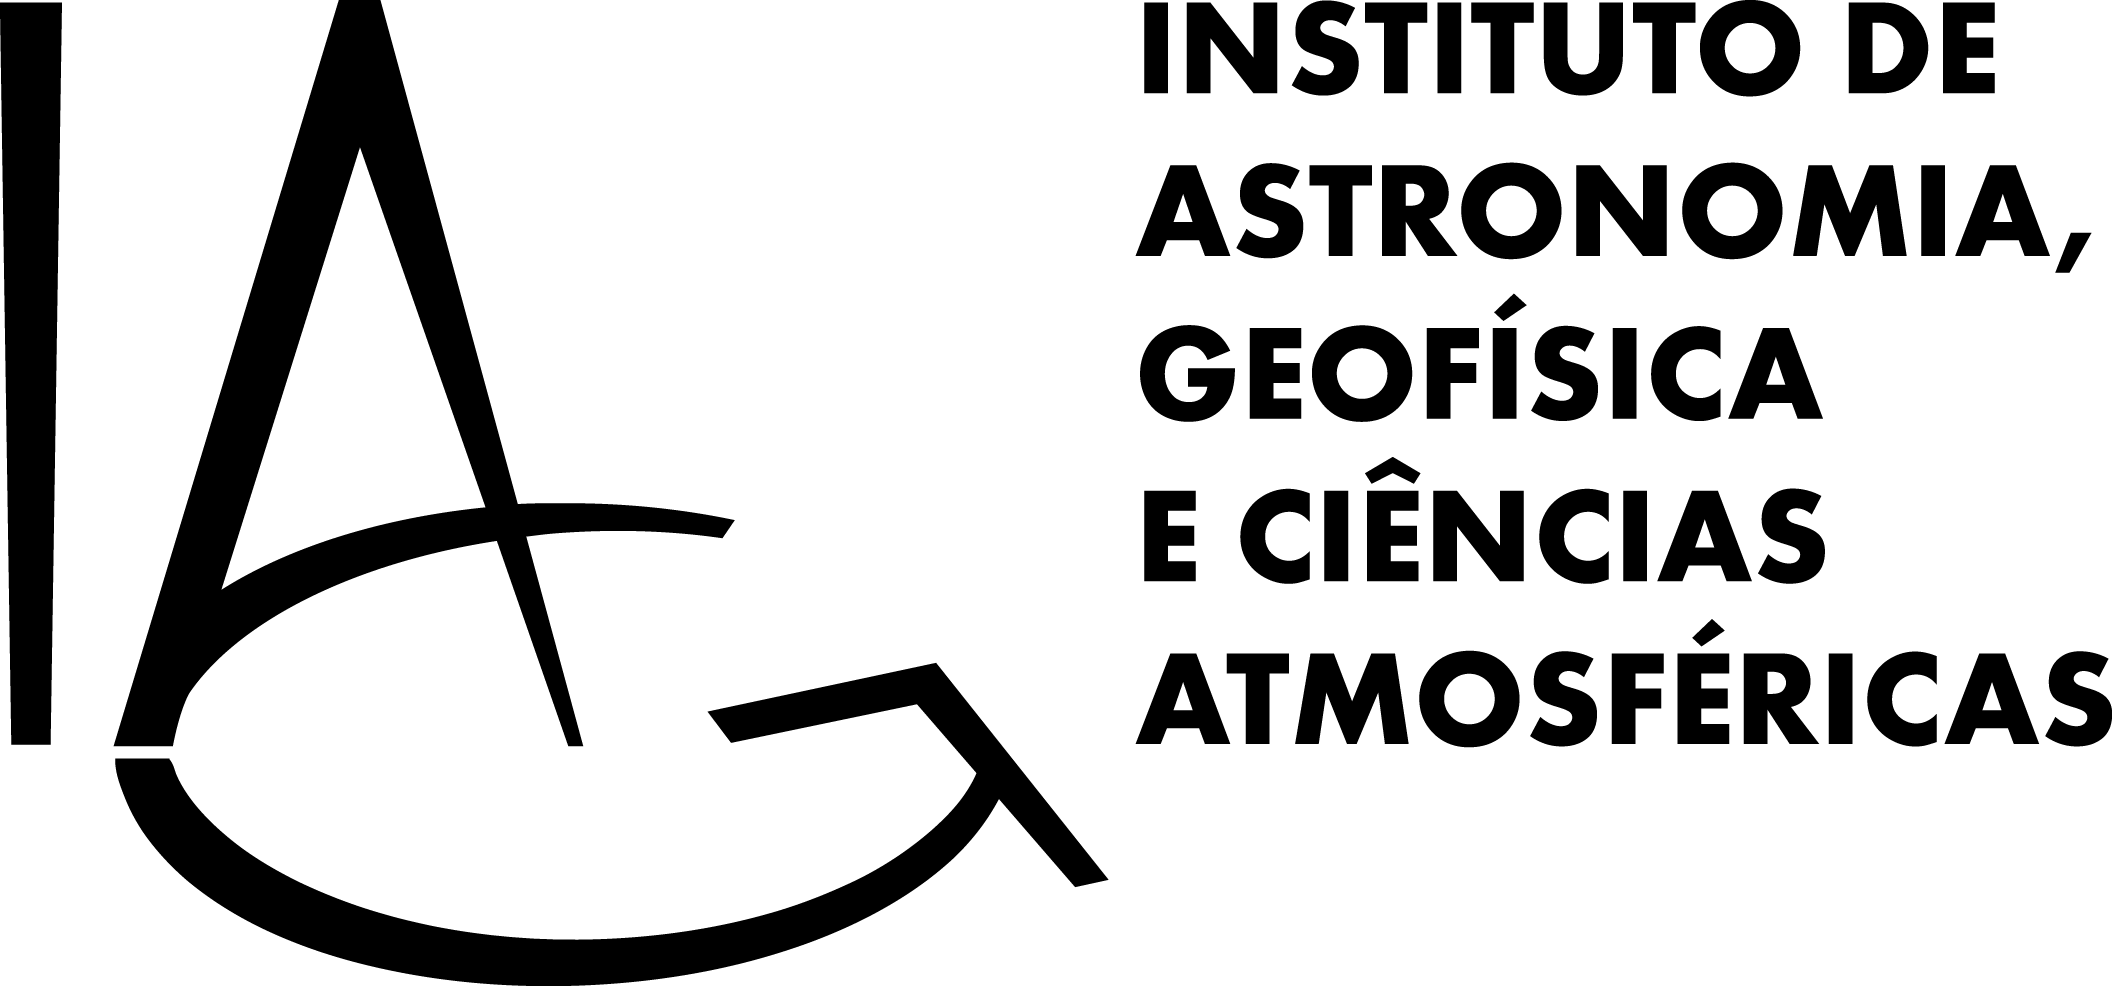
\includegraphics[height=1.5cm]{images/iag.png}
    \vspace{1cm}

    UNIVERSIDADE DE SÃO PAULO

    INSTITUTO DE ASTRONOMIA, GEOFÍSICA E CIÊNCIAS ATMOSFÉRICAS
    \vspace{4cm}

    TESE DE LIVRE DOCÊNCIA
    \vspace{2cm}

    {\huge\bfseries \ThesisTitle{}}
    \vspace{2cm}

    {\Large \ThesisAuthor}
    \vspace{4cm}

    {\small
      Tese apresentada para concurso títulos e provas visando a obtenção do

      título de Livre Docente junto ao Departamento de Geofísica do

      Instituto de Astronomia, Geofísica e Ciências Atmosféricas da

      Universidade de São Paulo.
      \vspace{1cm}

      Edital ATAc-IAG/005/2025
    }
    \vfill

    \ThesisYear{}
  \end{center}
\end{titlepage}


%==============================================================================

{\small

\vspace*{\fill}

\noindent
\textit{\ThesisTitle{}}.
\\[0.2cm]
\textcopyright{} Copyright \ThesisYear{} \ThesisAuthor{}
\\[0.2cm]
Last modified on \today.
\\[0.2cm]
DOI: \href{https://doi.org/\ThesisDOI}{\ThesisDOI}
\\[0.2cm]
Author ORCID: \href{https://orcid.org/\ORCID}{\ORCID}

\vspace{2.5cm}

\noindent
\textbf{\LARGE \faCreativeCommons{} \faCreativeCommonsBy{}}
\\
Available under the terms of the
\textbf{Creative Commons Attribution 4.0 Internacional} license.
\\
\url{https://creativecommons.org/licenses/by/4.0/deed}

\vspace{0.25cm}

\noindent
You are free to:

\begin{description}[labelindent=0.5cm]
    \item[Share ---]{
        Copy and redistribute the material in any medium or format for any
        purpose, even commercially.
    }
    \item[Adapt ---]{
        Remix, transform, and build upon the material for any purpose, even
        commercially.
    }
\end{description}

\vspace{0.25cm}

\noindent
Under the following terms:

\begin{description}[labelindent=0.5cm]
    \item[Attribution ---]{
        You must give appropriate credit, provide a link to the license, and
        indicate if changes were made. You may do so in any reasonable manner,
        but not in any way that suggests the licensor endorses you or your use.
    }
    \item[No additional restrictions ---]{
        You may not apply legal terms or technological measures that legally
        restrict others from doing anything the license permits.
}
\end{description}

\vspace{2cm}

}

%==============================================================================
\chapter*{Abstract}

Bla.

%==============================================================================
\tableofcontents

\mainmatter
\pagestyle{fancy}

%==============================================================================
\chapter{Introduction}

Bla.

%==============================================================================
\chapter{Gradient-boosted equivalent sources}

\begingroup
% Title, authors and affiliations
\newcommand{\Title}{Gradient-boosted equivalent sources}
\newcommand{\Soler}{Santiago R. Soler}
\newcommand{\SolerShort}{Soler}
\newcommand{\SolerMail}{santiago.r.soler@gmail.com}
\newcommand{\SolerORCID}{0000-0001-9202-5317}
\newcommand{\Uieda}{Leonardo Uieda}
\newcommand{\UiedaShort}{Uieda}
\newcommand{\UiedaORCID}{0000-0001-6123-9515}
\newcommand{\CONICET}{%
    Consejo Nacional de Investigaciones Científicas y Técnicas (CONICET),
    Ciudad Autónoma de Buenos Aires, Argentina
}
\newcommand{\IGSV}{%
    Instituto Geofísico Sismológico Volponi,
    Universidad Nacional de San Juan, San Juan, Argentina
}
\newcommand{\Liverpool}{%
    Department of Earth, Ocean and Ecological Sciences, School of Environmental
    Sciences, University of Liverpool, UK
}

% Publication-related variables
\newcommand{\Journal}{Geophysical Journal International}
\newcommand{\Year}{2021}

% DOIs
\newcommand{\PreprintDOI}{10.31223/X58G7C}
\newcommand{\DOI}{10.1093/gji/ggab297}
\newcommand{\DOILink}{\href{https://doi.org/\DOI}{doi.org/\DOI}}


% Keywords for GJI
\newcommand{\keywordsGJI}{%
Gravity anomalies and Earth structure;
Magnetic anomalies: modelling and interpretation;
Geopotential theory;
Inverse theory;
Statistical methods;
Australia.
}

% Define inverse symbol with shorter minus
\newcommand{\inv}{^{\text{-}1}}
\newcommand{\trans}{^{\text{T}}}

% Define some units
\renewcommand{\m}{$\,$m}
\renewcommand{\km}{$\,$km}
\newcommand{\mGal}{$\,$mGal}

% Import files with parameter values generated by notebooks
\newcommand{\NPrisms}{64}
\newcommand{\ModelEasting}{$111319 \, \text{m}$}
\newcommand{\ModelNorthing}{$111319 \, \text{m}$}
\newcommand{\ModelDepth}{$10000 \, \text{m}$}
\newcommand{\ModelMinDensity}{$-900 \, \text{kg} \, \text{m}^{-3}$}
\newcommand{\ModelMaxDensity}{$500 \, \text{kg} \, \text{m}^{-3}$}
\newcommand{\SurveyEasting}{$111319 \, \text{m}$}
\newcommand{\SurveyNorthing}{$110576 \, \text{m}$}
\newcommand{\SurveyNoise}{$1 \, \text{mGal}$}
\newcommand{\GroundSurveyPoints}{963}
\newcommand{\GroundSurveyMinHeight}{$0 \, \text{m}$}
\newcommand{\GroundSurveyMaxHeight}{$2052.2 \, \text{m}$}
\newcommand{\AirborneSurveyPoints}{5673}
\newcommand{\AirborneSurveyMinHeight}{$359 \, \text{m}$}
\newcommand{\AirborneSurveyMaxHeight}{$1255 \, \text{m}$}
\newcommand{\TargetHeight}{$2000 \, \text{m}$}
\newcommand{\TargetSpacing}{$2 \, \text{km}$}
\newcommand{\TargetEastingSize}{57}
\newcommand{\TargetNorthingSize}{56}
\newcommand{\GroundSourceBelowDataConstantDepthDamping}{10$^{-4}$, 10$^{-3}$,$\dots$, 10$^{2}$}
\newcommand{\GroundSourceBelowDataConstantDepthDepth}{1000 to 17000, step size 2000}
\newcommand{\GroundSourceBelowDataRelativeDepthDamping}{10$^{-4}$, 10$^{-3}$,$\dots$, 10$^{2}$}
\newcommand{\GroundSourceBelowDataRelativeDepthDepth}{1000 to 17000, step size 2000}
\newcommand{\GroundSourceBelowDataVariableDepthDamping}{10$^{-4}$, 10$^{-3}$,$\dots$, 10$^{2}$}
\newcommand{\GroundSourceBelowDataVariableDepthDepthFactor}{0.1, 0.5, 1, 2, 3, 4, 5 and 6}
\newcommand{\GroundSourceBelowDataVariableDepthDepth}{0 to 1400, step size 200}
\newcommand{\GroundSourceBelowDataVariableDepthKNearest}{1, 5, 10 and 15}
\newcommand{\GroundBlockAveragedSourcesConstantDepthDamping}{10$^{-4}$, 10$^{-3}$,$\dots$, 10$^{2}$}
\newcommand{\GroundBlockAveragedSourcesConstantDepthDepth}{1000 to 17000, step size 2000}
\newcommand{\GroundBlockAveragedSourcesConstantDepthSpacing}{1000, 2000, 3000 and 4000}
\newcommand{\GroundBlockAveragedSourcesRelativeDepthDamping}{10$^{-4}$, 10$^{-3}$,$\dots$, 10$^{2}$}
\newcommand{\GroundBlockAveragedSourcesRelativeDepthDepth}{1000 to 17000, step size 2000}
\newcommand{\GroundBlockAveragedSourcesRelativeDepthSpacing}{1000, 2000, 3000 and 4000}
\newcommand{\GroundBlockAveragedSourcesVariableDepthDamping}{10$^{-4}$, 10$^{-3}$,$\dots$, 10$^{2}$}
\newcommand{\GroundBlockAveragedSourcesVariableDepthSpacing}{1000, 2000, 3000 and 4000}
\newcommand{\GroundBlockAveragedSourcesVariableDepthDepthFactor}{0.1, 0.5, 1, 2, 3, 4, 5 and 6}
\newcommand{\GroundBlockAveragedSourcesVariableDepthDepth}{0 to 1400, step size 200}
\newcommand{\GroundBlockAveragedSourcesVariableDepthKNearest}{1, 5, 10 and 15}
\newcommand{\GroundGridSourcesConstantDepthDamping}{10$^{1}$, 10$^{2}$, 10$^{3}$ and 10$^{4}$}
\newcommand{\GroundGridSourcesConstantDepthDepth}{1000 to 9000, step size 2000}
\newcommand{\GroundGridSourcesConstantDepthSpacing}{1000, 2000, 3000 and 4000}
\newcommand{\AirborneSourceBelowDataConstantDepthDamping}{10$^{-4}$, 10$^{-3}$,$\dots$, 10$^{2}$}
\newcommand{\AirborneSourceBelowDataConstantDepthDepth}{1000 to 17000, step size 2000}
\newcommand{\AirborneSourceBelowDataRelativeDepthDamping}{10$^{-4}$, 10$^{-3}$,$\dots$, 10$^{2}$}
\newcommand{\AirborneSourceBelowDataRelativeDepthDepth}{1000 to 17000, step size 2000}
\newcommand{\AirborneSourceBelowDataVariableDepthDamping}{10$^{-4}$, 10$^{-3}$,$\dots$, 10$^{2}$}
\newcommand{\AirborneSourceBelowDataVariableDepthDepthFactor}{1 to 6, step size 1}
\newcommand{\AirborneSourceBelowDataVariableDepthDepth}{50 to 1450, step size 200}
\newcommand{\AirborneSourceBelowDataVariableDepthKNearest}{1, 5, 10 and 15}
\newcommand{\AirborneBlockAveragedSourcesConstantDepthDamping}{10$^{-4}$, 10$^{-3}$,$\dots$, 10$^{2}$}
\newcommand{\AirborneBlockAveragedSourcesConstantDepthDepth}{1000 to 17000, step size 2000}
\newcommand{\AirborneBlockAveragedSourcesConstantDepthSpacing}{1000, 2000, 3000 and 4000}
\newcommand{\AirborneBlockAveragedSourcesRelativeDepthDamping}{10$^{-4}$, 10$^{-3}$,$\dots$, 10$^{2}$}
\newcommand{\AirborneBlockAveragedSourcesRelativeDepthDepth}{1000 to 17000, step size 2000}
\newcommand{\AirborneBlockAveragedSourcesRelativeDepthSpacing}{1000, 2000, 3000 and 4000}
\newcommand{\AirborneBlockAveragedSourcesVariableDepthDamping}{10$^{-4}$, 10$^{-3}$,$\dots$, 10$^{2}$}
\newcommand{\AirborneBlockAveragedSourcesVariableDepthSpacing}{1000, 2000, 3000 and 4000}
\newcommand{\AirborneBlockAveragedSourcesVariableDepthDepthFactor}{1 to 6, step size 1}
\newcommand{\AirborneBlockAveragedSourcesVariableDepthDepth}{50 to 1450, step size 200}
\newcommand{\AirborneBlockAveragedSourcesVariableDepthKNearest}{1, 5, 10 and 15}
\newcommand{\AirborneGridSourcesConstantDepthDamping}{10$^{-3}$, 10$^{-2}$,$\dots$, 10$^{2}$}
\newcommand{\AirborneGridSourcesConstantDepthDepth}{1000 to 9000, step size 2000}
\newcommand{\AirborneGridSourcesConstantDepthSpacing}{1000, 2000 and 3000}
\newcommand{\BestGroundSourceBelowDataConstantDepthDamping}{10$^{-1}$}
\newcommand{\BestGroundSourceBelowDataConstantDepthDepth}{7000}
\newcommand{\BestGroundSourceBelowDataConstantDepthRms}{0.78}
\newcommand{\BestGroundSourceBelowDataConstantDepthNPoints}{963}
\newcommand{\BestGroundSourceBelowDataRelativeDepthDamping}{10$^{-1}$}
\newcommand{\BestGroundSourceBelowDataRelativeDepthDepth}{9000}
\newcommand{\BestGroundSourceBelowDataRelativeDepthRms}{0.79}
\newcommand{\BestGroundSourceBelowDataRelativeDepthNPoints}{963}
\newcommand{\BestGroundSourceBelowDataVariableDepthDamping}{1}
\newcommand{\BestGroundSourceBelowDataVariableDepthDepthFactor}{1}
\newcommand{\BestGroundSourceBelowDataVariableDepthDepth}{1000}
\newcommand{\BestGroundSourceBelowDataVariableDepthKNearest}{15}
\newcommand{\BestGroundSourceBelowDataVariableDepthRms}{0.80}
\newcommand{\BestGroundSourceBelowDataVariableDepthNPoints}{963}
\newcommand{\BestGroundBlockAveragedSourcesConstantDepthDamping}{10$^{-1}$}
\newcommand{\BestGroundBlockAveragedSourcesConstantDepthDepth}{7000}
\newcommand{\BestGroundBlockAveragedSourcesConstantDepthSpacing}{3000}
\newcommand{\BestGroundBlockAveragedSourcesConstantDepthRms}{0.77}
\newcommand{\BestGroundBlockAveragedSourcesConstantDepthNPoints}{518}
\newcommand{\BestGroundBlockAveragedSourcesRelativeDepthDamping}{10$^{-1}$}
\newcommand{\BestGroundBlockAveragedSourcesRelativeDepthDepth}{7000}
\newcommand{\BestGroundBlockAveragedSourcesRelativeDepthSpacing}{3000}
\newcommand{\BestGroundBlockAveragedSourcesRelativeDepthRms}{0.79}
\newcommand{\BestGroundBlockAveragedSourcesRelativeDepthNPoints}{518}
\newcommand{\BestGroundBlockAveragedSourcesVariableDepthDamping}{10$^{-1}$}
\newcommand{\BestGroundBlockAveragedSourcesVariableDepthSpacing}{3000}
\newcommand{\BestGroundBlockAveragedSourcesVariableDepthDepthFactor}{1}
\newcommand{\BestGroundBlockAveragedSourcesVariableDepthDepth}{600}
\newcommand{\BestGroundBlockAveragedSourcesVariableDepthKNearest}{15}
\newcommand{\BestGroundBlockAveragedSourcesVariableDepthRms}{0.72}
\newcommand{\BestGroundBlockAveragedSourcesVariableDepthNPoints}{518}
\newcommand{\BestGroundGridSourcesConstantDepthDamping}{10$^{2}$}
\newcommand{\BestGroundGridSourcesConstantDepthDepth}{3000}
\newcommand{\BestGroundGridSourcesConstantDepthSpacing}{2000}
\newcommand{\BestGroundGridSourcesConstantDepthRms}{0.97}
\newcommand{\BestGroundGridSourcesConstantDepthNPoints}{3192}
\newcommand{\BestAirborneSourceBelowDataConstantDepthDamping}{10$^{-2}$}
\newcommand{\BestAirborneSourceBelowDataConstantDepthDepth}{7000}
\newcommand{\BestAirborneSourceBelowDataConstantDepthRms}{0.35}
\newcommand{\BestAirborneSourceBelowDataConstantDepthNPoints}{5673}
\newcommand{\BestAirborneSourceBelowDataRelativeDepthDamping}{10$^{-2}$}
\newcommand{\BestAirborneSourceBelowDataRelativeDepthDepth}{9000}
\newcommand{\BestAirborneSourceBelowDataRelativeDepthRms}{0.35}
\newcommand{\BestAirborneSourceBelowDataRelativeDepthNPoints}{5673}
\newcommand{\BestAirborneSourceBelowDataVariableDepthDamping}{1}
\newcommand{\BestAirborneSourceBelowDataVariableDepthDepthFactor}{1}
\newcommand{\BestAirborneSourceBelowDataVariableDepthDepth}{1450}
\newcommand{\BestAirborneSourceBelowDataVariableDepthKNearest}{15}
\newcommand{\BestAirborneSourceBelowDataVariableDepthRms}{0.36}
\newcommand{\BestAirborneSourceBelowDataVariableDepthNPoints}{5673}
\newcommand{\BestAirborneBlockAveragedSourcesConstantDepthDamping}{10$^{-4}$}
\newcommand{\BestAirborneBlockAveragedSourcesConstantDepthDepth}{9000}
\newcommand{\BestAirborneBlockAveragedSourcesConstantDepthSpacing}{3000}
\newcommand{\BestAirborneBlockAveragedSourcesConstantDepthRms}{0.34}
\newcommand{\BestAirborneBlockAveragedSourcesConstantDepthNPoints}{1100}
\newcommand{\BestAirborneBlockAveragedSourcesRelativeDepthDamping}{10$^{-3}$}
\newcommand{\BestAirborneBlockAveragedSourcesRelativeDepthDepth}{9000}
\newcommand{\BestAirborneBlockAveragedSourcesRelativeDepthSpacing}{2000}
\newcommand{\BestAirborneBlockAveragedSourcesRelativeDepthRms}{0.34}
\newcommand{\BestAirborneBlockAveragedSourcesRelativeDepthNPoints}{1663}
\newcommand{\BestAirborneBlockAveragedSourcesVariableDepthDamping}{10$^{-2}$}
\newcommand{\BestAirborneBlockAveragedSourcesVariableDepthSpacing}{2000}
\newcommand{\BestAirborneBlockAveragedSourcesVariableDepthDepthFactor}{2}
\newcommand{\BestAirborneBlockAveragedSourcesVariableDepthDepth}{50}
\newcommand{\BestAirborneBlockAveragedSourcesVariableDepthKNearest}{15}
\newcommand{\BestAirborneBlockAveragedSourcesVariableDepthRms}{0.33}
\newcommand{\BestAirborneBlockAveragedSourcesVariableDepthNPoints}{1663}
\newcommand{\BestAirborneGridSourcesConstantDepthDamping}{10$^{-1}$}
\newcommand{\BestAirborneGridSourcesConstantDepthDepth}{7000}
\newcommand{\BestAirborneGridSourcesConstantDepthSpacing}{1000}
\newcommand{\BestAirborneGridSourcesConstantDepthRms}{0.34}
\newcommand{\BestAirborneGridSourcesConstantDepthNPoints}{12544}
\newcommand{\SourceLayoutsSchematicsObservations}{166}
\newcommand{\SourceLayoutsSchematicsSourceBelowData}{166}
\newcommand{\SourceLayoutsSchematicsGridSources}{378}
\newcommand{\SourceLayoutsSchematicsBlockAveragedSources}{87}
\newcommand{\BoostOverlappingWindowSize}{$30000 \, \text{m}$}
\newcommand{\EqlBoostAirborneRmsScore}{$0.38 \, \text{mGal}$}
\newcommand{\EqlBoostAirborneDepth}{$3000 \, \text{m}$}
\newcommand{\EqlBoostAirborneDamping}{0.1}
\newcommand{\EqlBoostAirborneSpacing}{$2 \, \text{km}$}
\newcommand{\EqlBoostAirborneWindowSize}{$20 \, \text{km}$}
\newcommand{\EqlBoostAirborneNSources}{1663}
\newcommand{\EqlBoostAirborneMinDepth}{$1000 \, \text{m}$}
\newcommand{\EqlBoostAirborneMaxDepth}{$19000 \, \text{m}$}
\newcommand{\EqlBoostAirborneMinDamping}{1e-06}
\newcommand{\EqlBoostAirborneMaxDamping}{10}
\newcommand{\AustraliaSmallAreaEastingSize}{$300 \, \text{km}$}
\newcommand{\AustraliaSmallAreaNorthingSize}{$300 \, \text{km}$}
\newcommand{\AustraliaSmallAreaNPoints}{14934}
\newcommand{\AustraliaDepthMin}{$1000 \, \text{m}$}
\newcommand{\AustraliaDepthMax}{$15000 \, \text{m}$}
\newcommand{\AustraliaDampingMin}{0.01}
\newcommand{\AustraliaDampingMax}{10000}
\newcommand{\AustraliaEqlDepth}{$3000 \, \text{m}$}
\newcommand{\AustraliaEqlDamping}{100}
\newcommand{\AustraliaEqlSpacing}{$1800 \, \text{m}$}
\newcommand{\AustraliaEqlWindowSize}{$225 \, \text{km}$}
\newcommand{\AustraliaEqlRmsScore}{$1.33 \, \text{mGal}$}
\newcommand{\AustraliaEqlNSources}{796744}
\newcommand{\AustraliaEqlGridNLongitude}{2442}
\newcommand{\AustraliaEqlGridNLatitude}{2085}
\newcommand{\AustraliaEqlGridHeight}{$2127.58 \, \text{m}$}



\begin{summarybox}
    \noindent
    This chapter was originally published as
    \textbf{``Soler, S. R. and Uieda, L. (\Year). \Title{}. \textit{\Journal{}}.
    doi:\href{https://doi.org/\DOI}{\DOI}.''}, which was previously published
    as a preprint on EarthArXiv (\url{https://doi.org/\PreprintDOI}) under the
    terms of the CC-BY license. It is reproduced here under these terms.
\end{summarybox}

\section*{Abstract}
The equivalent source technique is a powerful and widely used method for
processing gravity and magnetic data.  Nevertheless, its major
drawback is the large computational cost in terms of processing time and
computer memory.
We present two techniques for reducing the computational cost of equivalent
source processing: block-averaging source locations and the
gradient-boosted equivalent source algorithm.
Through block-averaging, we reduce the number of source coefficients that
must be estimated while retaining the minimum desired resolution in the final
processed data.
With the gradient boosting method, we estimate the sources coefficients in
small batches along overlapping windows, allowing us to reduce the computer
memory requirements arbitrarily to conform to the constraints of the
available hardware.
We show that the combination of block-averaging and gradient-boosted
equivalent sources is capable of producing accurate interpolations through
tests against synthetic data.
Moreover, we demonstrate the feasibility of our method by gridding a gravity
dataset covering Australia with over 1.7 million observations using a modest
personal computer.


% \section{Introduction}

Measurements of anomalies in potential fields, like gravity disturbances and
total-field magnetic anomalies, are widely used in geophysical exploration for
their low cost of acquisition.
These data can be surveyed using ground, airborne, shipborne, or satellite
systems.
During ground surveys, the data are often gathered following irregular paths or
networks along the surface of the terrain, leading to highly variable
elevations in mountainous regions.
Airborne and satellite surveys gather data along flight lines, producing
closely spaced measurements along almost straight lines but with larger spacing
between adjacent lines.
Measurement height can also change because of the vertical movement of the
aircraft.
Processing of the data often involves interpolation onto a regular grid at
constant height, both to improve visualization for interpretation purposes as
well as to prepare the data for further processing and modelling (e.g.,
reduction-to-the-pole, derivative calculations, upward continuation, Euler
deconvolution).

Several methods exist in the literature for interpolation in two dimensions,
for example continuous curvature splines in tension \citep{smith1990},
bi-harmonic (thin-plate) splines \citep{sandwell1987}, and kriging
\citep{hansen1993}.
These general-purpose methods have limitations when it comes to interpolating
potential field data, namely
(i)~they are not able to take into account the variable height of the
observation points and
(ii)~the interpolating functions are not necessarily harmonic, which
is the underlying assumption behind many processing techniques
(e.g., upward continuation and vertical derivatives).

A widely used method for interpolating gravity and magnetic data
is the equivalent sources technique (also known as equivalent layer, radial
basis functions, or Green's functions interpolation).
First introduced by \citet{dampney1969}, the method consists in fitting a model
of finite elementary sources to the data and using this model to predict new
data values.
Besides interpolation, equivalent sources have been used for
reduction-to-the-pole of magnetic data
\citep{silva1986, nakatsuka2006, Guspi2009}, upward
continuation \citep{emilia1973, Li2010}, joint processing of gravity gradient
data \citep{barnes2011}, modelling the lithospheric magnetic field
\citep{kother2015}, recovering the magnetic induction vector from
total-field magnetic anomalies \citep{li2020}, and more.

It is also worth mentioning the least-squares collocation method
(LSC), which is widely used in geodesy
\citep[][and references therein]{tscherning2015}.
LCS is often applied to combine and interpolate different linear functionals of
the disturbing gravity potential (gravity anomalies, gravity disturbances,
deflections of the vertical, geoid height, et cetera).
Like equivalent sources, collocation also requires the solution of a large
linear system of the order of the number of observed data.
As such, it's practical application suffers from the same computational
challenges.

Many variants of the equivalent sources technique have been proposed, often
attempting to obtain faster or more accurate solutions.
The key factors that vary between them are: (i) the type of source, (ii)
the location of the sources, and (iii) the solution strategy.

The most commonly used type of source is a point mass for gravity or dipole for
magnetics \citep[e.g.,~][]{vonfrese1981, silva1986, Mendona1994,
Siqueira2017}.
However, right-rectangular prisms \citep[e.g.,][]{barnes2011, Jirigalatu2019,
li2020} and tesseroids \citep{bouman2016} have also been used successfully.
In fact, even point sources with a simple inverse distance function, instead of
actual gravity or magnetic fields, can be used as
equivalent sources \citep{cordell1992}.

The location of sources often follows one of two strategies.
The most common approach is to distribute sources on a regular grid at a
constant depth \citep[e.g.,~][]{Leao1989, barnes2011, OliveiraJr2013}.
Alternatively, sources can be placed beneath each data point
\citep[e.g.,~][]{cordell1992, Siqueira2017}.
Some recent work by \citet{li2020} places the sources in two overlapping layers
at different depths.

The coefficients of the equivalent source model are often estimated through
damped least-squares.
This imposes a heavy computational load when the number of data points is
large (e.g., airborne and satellite surveys).
To reduce the computational load, \citet{Mendona1994} built the solution
iteratively by incorporating one data point at a time using the ``equivalent
data concept''.
\citet{Leao1989} processed the input data using a moving window, only fitting the
data inside the window and predicting observations at its center.
\citet{Li2010} and \citet{barnes2011} apply different operations to generate a
sparse representation of the sensitive matrix (respectively, wavelet
compression and quadtree discretization), which significantly improves the
speed of the least-squares solution.
\citet{OliveiraJr2013} parametrized the equivalent layer as a piecewise bivariate
polynomial function, reducing the number of parameters in the solution.
\citet{Siqueira2017} developed an iterative solution in which the sensitivity
matrix is transformed into a diagonal matrix with constant terms through the
``excess mass criterion''.
\citet{Jirigalatu2019} applied the Gauss-FFT method to speed up the forward
modelling operations and solved the least-squares problem using steepest
descent to avoid calculating the Hessian matrix and solving linear systems.

Many of the existing methods solve under-determined problems, requiring a much
larger number of equivalent sources than the number of data points.
Some achieve greater efficiency by restricting their applications
to specific data types \citep{Siqueira2017},
interpolating only on regular grids \citep{Leao1989},
or requiring already gridded data \citep{takahashi2020},
to name a few.
Furthermore, many of the optimizations proposed are also complex to implement
in a computer program, limiting their wider adoption.

In the present study,
we propose two strategies for reducing the computational load of
the equivalent sources technique:

\begin{enumerate}
    \item Reduce the number of equivalent sources for oversampled surveys
      through a \emph{block-averaging} strategy while maintaining the quality
      of the solution.
    \item Fit the equivalent source model iteratively along overlapping windows
      using a \emph{gradient boosting} algorithm \citep{friedman2001}.
\end{enumerate}

The first strategy consists in dividing the survey area into horizontal blocks
and assigning a single source to each block, located at the median horizontal
location of the data points.
For airborne, shipborne, and satellite surveys, which are oversampled along
tracks, this can greatly reduce the size of the inverse problem while retaining
the same quality of interpolation.

The gradient boosting algorithm allows us to fit the equivalent source model
iteratively by operating on individual overlapping windows.
As a result, our method solves several much smaller least-squares problems
instead of a large one.
This has some similarities with the strategy used by \citet{Leao1989} but
without the requirement for sources and predictions to be on regular grids.

Through tests on synthetic data, we show that:
(i)~the \emph{block-averaged} sources are able to achieve the same accuracy as
other traditional equivalent source layouts while using a fraction of the
number of sources, and
(ii)~the \emph{gradient boosting} algorithm greatly reduces the computational
memory required to fit very large datasets without sacrificing prediction
accuracy.
Finally, a combination of both strategies is used to process a collection of
approximately 1.7 million ground gravity data measurements from Australia.

%%%%%%%%%%%%%%%%%%%%%%%%%%%%%%%%%%%%%%%%%%%%%%%%%%%%%%%%%%%%%%%%%%%%%%%%%%%%%%%

\section{Methodology}

\subsection{The equivalent sources technique}

We will follow the ``generalized equivalent sources'' of \citet{cordell1992}
and assume that any harmonic function $d(\mathbf{p})$ can be approximated by a
sum of $M$ discrete point source effects

\begin{equation}
    d(\mathbf{p})
    =
    \sum\limits_{j=1}^{M} \frac{c_j}{\left\lVert \mathbf{p} - \mathbf{q}_j
    \right\rVert} \ ,
    \label{eq:eql-forward}
\end{equation}

\noindent in which
$\mathbf{p}$ and $\mathbf{q}_j$ are, respectively, the position vectors in a 3D
Cartesian space of data and sources,
$c_j$ is a scalar coefficient related to the point source located at
$\mathbf{q}_j$,
and $\lVert \cdot \rVert$ represents the $\text{L}_2$ norm.
The horizontal and vertical distribution of sources is discussed in
section~\ref{sec:source_distribution}.

In case we have values of the harmonic function at $N$ discrete points
$\{\mathbf{p}_1\ \mathbf{p}_2\ \ldots\ \mathbf{p}_N\}$,
we can write a set of $N$ equations of the form

\begin{equation}
    d_i
    =
    \sum\limits_{j=1}^{M} \frac{c_j}{\left\lVert \mathbf{p}_i - \mathbf{q}_j
    \right\rVert}
    \quad \forall i=1,2,\ldots,N
    \ ,
    \label{eq:forward-sum}
\end{equation}

\noindent where $d_i$ is the calculated value at point $\mathbf{p}_i$.
These equations can also be expressed in matrix form as

\begin{equation}
    \mathbf{d} = \mathbf{A} \mathbf{c} \ ,
    \label{eq:linear-problem}
\end{equation}

\noindent where $\mathbf{d}$ is a column vector containing the $N$ predicted
values at the observation points,
$\mathbf{c}$ is a column vector containing the $M$ coefficients $c_j$,
and $\mathbf{A}$ is the $N \times M$ Jacobian matrix,
whose elements are

\begin{equation}
    a_{ij} = \frac{1}{\left\lVert\mathbf{p}_i - \mathbf{q}_j\right\rVert}
\end{equation}

For a given set of $N$ observed data $\mathbf{d}^o$,
we can find a least-squares solution to
Eq.~\ref{eq:linear-problem} and obtain the values of
$\mathbf{c}$ that best fit the observations.
These coefficients can, in turn, be used to predict the value of the harmonic
function at any other point outside of the sources by evaluating
Eq.~\ref{eq:eql-forward}.
Gridding and upward continuation can thus be achieved by predicting values on
points that fall on a regular grid or at different heights, respectively.


\subsection{Damped least-squares solution}
\label{sec:eql_inversion}

We can obtain the values of the source coefficients $\mathbf{c}$ that best
fit the observed field values $\mathbf{d}^o$ by minimizing the goal function

\begin{equation}
    \phi(\mathbf{c}) =
    \left[\mathbf{d}^o - \mathbf{A}\mathbf{c}\right]\trans
    \mathbf{W}
    \left[\mathbf{d}^o - \mathbf{A}\mathbf{c}\right]
    + \lambda_d\ \mathbf{c}\trans\mathbf{c}
    \ ,
    \label{eq:misfit-unscaled}
\end{equation}

\noindent where
$\mathbf{W}$ is a $N \times N$ diagonal matrix of data weights and
$\lambda_d$ is a positive \emph{damping} parameter with the same units as the
Jacobian matrix elements.
The second term on the right-hand side of Eq.~\ref{eq:misfit-unscaled} is the
zeroth-order Tikhonov regularization \citep{tikhonov1977}, also known as a
damping regularization, that is used to stabilize the solution.

The damping parameter controls the amount of regularization that will be
applied.
An overly large value would generate a smooth solution that fails to reproduce
the high frequency components of the data, while an overly small value would
result in over-fitting, thus failing to produce realistic interpolation results
\citep{martinez2016}.
The range of acceptable values for the damping parameter $\lambda_d$ will
depend on the values of the Jacobian matrix $\mathbf{A}$ and the coefficients.
Consequently, this range will vary (often dramatically) between datasets,
making it difficult to choose an appropriate value in practice.

To solve this issue, we first scale the Jacobian matrix so that its elements
are dimensionless and each column has unit variance.
We define a diagonal matrix $\mathbf{S}$

\begin{equation}
    \mathbf{S} =
    \begin{bmatrix}
      \sigma_1 & 0 & \cdots &0 \\
      0 & \sigma_2 & \cdots &0 \\
      \vdots & \vdots & \ddots & \vdots \\
      0  & 0 & \cdots & \sigma_M
    \end{bmatrix}_{M \times M}
    ,
\end{equation}

\noindent in which $\sigma_j$ is the standard deviation of the $j$-th column of
$\mathbf{A}$.
We then write the forward problem in Eq.~\ref{eq:linear-problem} as

\begin{equation}
    \mathbf{d}
    =
    \mathbf{A} \mathbf{S}\inv \mathbf{S} \mathbf{c}
    =
    \left[
        \mathbf{A} \mathbf{S}\inv
    \right]
    \left[
        \mathbf{S} \mathbf{c}
    \right]
    =
    \mathbf{B} \mathbf{m}
\end{equation}

\noindent where $\mathbf{B} = \mathbf{A} \mathbf{S}\inv$ is the scaled and
dimensionless Jacobian matrix
and $\mathbf{m} = \mathbf{S} \mathbf{c}$ is a vector containing scaled
coefficients with the same units as the data.

The goal function defined in Eq.~\ref{eq:misfit-unscaled} can be
rewritten as

\begin{equation}
    \phi(\mathbf{m}) =
    \left[\mathbf{d}^o - \mathbf{B}\mathbf{m}\right]\trans
    \mathbf{W}
    \left[\mathbf{d}^o - \mathbf{B}\mathbf{m}\right]
    + \lambda\ \mathbf{m}\trans\mathbf{m}
    \ ,
    \label{eq:misfit}
\end{equation}

\noindent where $\lambda$ is a \emph{dimensionless} damping parameter and
regularization is applied on the scaled coefficients $\mathbf{m}$ instead of
$\mathbf{c}$.
Using a dimensionless damping parameter allows us to narrow the range of values
of $\lambda$ that would generate the most accurate predictions, irrespective
of the dataset and its units.
From experience, we recommend searching for suitable $\lambda$ values between
$10^{-6}$ and $10^{4}$ varying by order-of-magnitude.
The choice of the damping and other hyper-parameters, like the source depth,
could be done through well-established statistical methods, such as
cross-validation.

The vector of scaled coefficients $\hat{\mathbf{m}}$ that minimizes the goal
function can be found by solving the \emph{normal equation system}
\citep{menke1989}

\begin{equation}
    \left[
      \mathbf{B}\trans \mathbf{W} \mathbf{B} + \lambda \mathbf{I}
    \right]
    \hat{\mathbf{m}} =
    \mathbf{B}\trans\mathbf{W}
    \mathbf{d}^o.
    \label{eq:least_squares_solution}
\end{equation}

Once the scaled coefficients are obtained, the estimated unscaled coefficients
$\hat{\mathbf{c}}$ can be calculated by removing the scaling factor

\begin{equation}
    \hat{\mathbf{c}} = \mathbf{S}\inv \hat{\mathbf{m}} \ .
\end{equation}

\noindent The forward modeling operations used to perform predictions
(e.g., for interpolation and upward continuation) are left unchanged by
using vector $\hat{\mathbf{c}}$ instead of $\hat{\mathbf{m}}$.


\subsection{Gradient boosting}

Gradient boosting was first introduced by \citet{friedman2001, friedman2002} as
a method for fitting additive parametric models of the form

\begin{equation}
    d = \sum_{k=1}^K \alpha_k f(\mathbf{c}_k),
\end{equation}

\noindent where $\alpha_k$ is a scalar coefficient called the \emph{step-size}
and $f$ is a function of the parameter vector $\mathbf{c}_k$.
For linear problems, these additive models can be written as the matrix
equation

\begin{equation}
    \mathbf{d} = \sum_{k=1}^K \mathbf{A}_k \mathbf{c}_k \ .
    \label{eq:gb-linear-model}
\end{equation}

\noindent Because of the linearity of the $f(\mathbf{c}_k)$ functions, the
$\alpha_k$ step-size parameters can be incorporated into the parameter vector
$\mathbf{c}_k$.

We can transform our equivalent source problem in
Eq.~\ref{eq:linear-problem} into an additive model by following these
steps:

\begin{enumerate}
  \item Define a set of $M$ equivalent sources distributed throughout the
    survey area (see section \ref{sec:source_distribution} for details).
  \item Define a set of $K$ overlapping windows of equal size that cover the
    survey area.
  \item Create $K$ separate sets of equivalent sources, one for each window.
    Each set will be formed by the portion of the original $M$ sources that
    fall inside the respective window.
    Since the windows overlap, the total number of sources from all sets will
    be greater than $M$.
  \item Define vector $\mathbf{c}_k$ as the $M_k$ coefficients of the
    equivalent sources of the $k$-th window.
  \item Define matrix $\mathbf{A}_k$ as the $N \times M_k$ Jacobian matrix
    between the sources in the $k$-th window and all $N$ data points of the
    survey.
  \item Model the predicted data as a superposition of the effects of the $K$
    separate sets of equivalent sources (i.e., Eq.~\ref{eq:gb-linear-model}).
\end{enumerate}

The gradient boosting algorithm works by fitting each component of the
additive model, one at a time, to the residuals of the previous component.
\citet{friedman2001} demonstrates that this corresponds to a steepest-descent
optimization in the so-called ``function space''.
The adaptation of the gradient boosting method to find the damped least-squares
solutions for the $K$ parameter vectors $\mathbf{c}_k$ in
Eq.~\ref{eq:gb-linear-model} is presented in
Algorithm~\ref{alg:gradient_boosting}.

\begin{algorithm}[!h]
  \DontPrintSemicolon
  \setstretch{1.5}
  Define the residual vector $\mathbf{r}_{0} = \mathbf{d}^o$ \;
  \For{ $k = 1$ \KwTo $K$ }{


    Calculate the $N \times M_k$ Jacobian matrix $\mathbf{A}_k$
    \;

    $\mathbf{B}_k = \mathbf{A}_k \mathbf{S}_k\inv$
    \nllabel{alg:scale}
    \;

    $
     \hat{\mathbf{m}}_k = \left[\mathbf{B}_k\trans \mathbf{W}_k \mathbf{B}_k +
     \lambda \mathbf{I} \right]\inv \mathbf{B}_k\trans \mathbf{W}_k
     \mathbf{r}_{k-1}
    $
    \nllabel{alg:fit}
    \;

    $\hat{\mathbf{c}}_k = \mathbf{S}_k\inv \hat{\mathbf{m}}_k$
    \nllabel{alg:unscale}
    \;

    $\mathbf{d}_k = \mathbf{A}_k \hat{\mathbf{c}}_k$
    \nllabel{alg:predicted}
    \;

    $\mathbf{r}_k = \mathbf{r}_{k - 1} - \mathbf{d}_k$
    \nllabel{alg:residual}
    \;
  }
  \BlankLine
  \setstretch{1}
  \caption{Gradient boosting solution for damped least-squares regression.}
  \label{alg:gradient_boosting}
\end{algorithm}

After all $\mathbf{c}_k$ coefficients vectors are estimated, we can predict the
effect of the additive equivalent source model on any point through the
summation

\begin{equation}
    d(\mathbf{p}) =
    \sum\limits_{k=1}^K \sum\limits_{j=1}^{M_k}
    \frac{{c_k}_j}{\left\lVert \mathbf{p} - {\mathbf{q}_k}_j \right\rVert}
    \ ,
    \label{eq:eql-forward-gb}
\end{equation}

\noindent
in which ${c_k}_j$ is the $j$-th element of the $\mathbf{c}_k$ vector and the
${\mathbf{q}_k}_j$ is the position vector of the $j$-th source of the $k$-th
window.

To improve the convergence of the algorithm, \citet{friedman2002} suggests
introducing randomness into the fitting process. We achieve this by randomizing
the order in which the $K$ windows are used in the gradient boosting algorithm.
Section~\ref{sec:gb_interpolation} explores the effect of randomization in the
convergence rate of the algorithm and the accuracy of the interpolation.

The $\mathbf{A}_k$ matrices have only $N \times M_k$ elements
(where $M_k$ is the number sources on the $k-$th window), which can be
considerably smaller than the $N \times M$ elements of $\mathbf{A}$.
Therefore, the gradient boosting method allows us to fit
equivalent source models that would produce Jacobian matrices that are larger
than the available computer memory.
Furthermore, we can increase or decrease the size of the overlapping windows as
needed depending on the number of sources in the model and the available
computer memory.

We can improve the efficiency of the algorithm further by:

\begin{enumerate}
  \item Using only the $N_k$ data points that fall within the $k$-th window for
    fitting the sources (steps \ref{alg:scale} and \ref{alg:fit} of
    algorithm~\ref{alg:gradient_boosting}).
    By doing so, we can replace the $N \times M_k$ Jacobian matrix $\mathbf{A}_k$
    with the smaller $N_k \times M_k$ matrix $\tilde{\mathbf{A}}_k$.
    We still use all $N$ data points when calculating the predicted data and
    residuals (steps \ref{alg:predicted} and \ref{alg:residual} of
    algorithm~\ref{alg:gradient_boosting}).
  \item The forward modeling operation performed in step \ref{alg:predicted}
    can be done by a summation (Eq.~\ref{eq:forward-sum}) instead of a
    matrix-vector product, which allows us to avoid computing and storing the
    larger $N \times M_k$ matrix $\mathbf{A}_k$ at any point.
\end{enumerate}

Algorithm~\ref{alg:gradient_boosting_window} is the final
\textit{gradient-boosted equivalent sources algorithm} which incorporates these
changes.
Figure~\ref{fig:gradient-boosting-schematics} shows a sketch of the algorithm
steps applied a set of observation points that simulate a ground survey and
locating one source below each data point.

\begin{algorithm}[!h]
  \DontPrintSemicolon
  \setstretch{1.5}
  Define the residual vector $\mathbf{r}_{0} = \mathbf{d}^o$ \;
  \For{ $k = 1$ \KwTo $K$ }{

    Select weights $\tilde{\mathbf{W}}_k$ and residuals
    $\tilde{\mathbf{r}}_{k - 1}$ for data points inside the $k$-th window
    \;

    Calculate Jacobian matrix $\tilde{\mathbf{A}}_k$ with data points and
    sources inside the $k$-th window
    \;

    $\mathbf{B}_k = \tilde{\mathbf{A}}_k \mathbf{S}_k\inv$
    \;

    $
     \hat{\mathbf{m}}_k = \left[
     \mathbf{B}_k\trans \tilde{\mathbf{W}}_k \mathbf{B}_k +
     \lambda \mathbf{I} \right]\inv \mathbf{B}_k\trans \tilde{\mathbf{W}}_k
     \tilde{\mathbf{r}}_{k-1}
    $
    \;

    $\hat{\mathbf{c}}_k = \mathbf{S}_k\inv \hat{\mathbf{m}}_k$
    \;

    Calculate $ \mathbf{d}_k $, where
    $
    {d_k}_i
    =
    \sum\limits_{j=1}^{M_k} \dfrac{{c_k}_j}{\left\lVert \mathbf{p}_i -
        {\mathbf{q}_k}_j
    \right\rVert}
    \quad \forall\ i=1\ \text{to}\ N
    $
    \;

    $\mathbf{r}_k = \mathbf{r}_{k - 1} - \mathbf{d}_k$
    \;
  }
  \BlankLine
  \setstretch{1}
  \caption{Gradient-boosted equivalent sources algorithm.}
  \label{alg:gradient_boosting_window}
\end{algorithm}

\begin{figure*}[tb!]
    \centering
    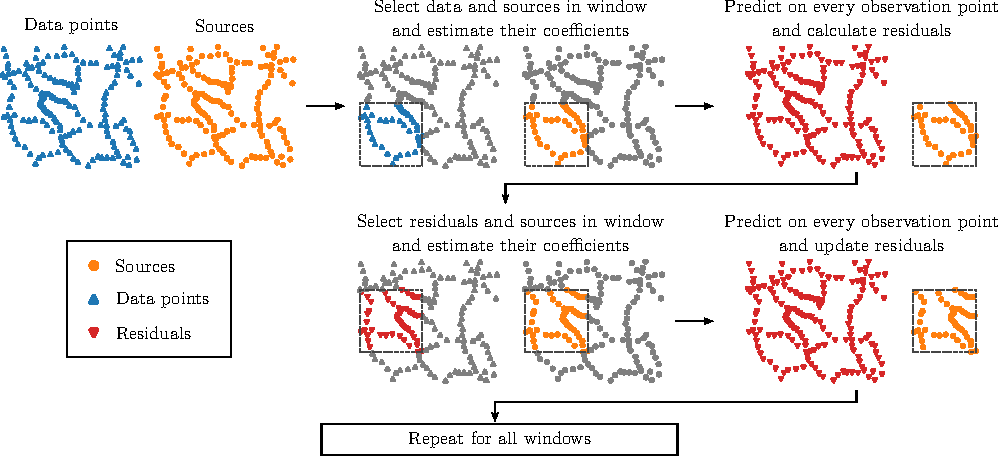
\includegraphics[width=\linewidth]{eql-gradient-boosted/figs/gradient-boosting-schematics.pdf}
    \caption{
        Sketch of the gradient-boosted equivalent source algorithm.
        Data points are represented by blue upwards-facing triangles,
        equivalent sources by orange dots, data residuals by red downwards-facing
        triangles, and the current window by black dashed lines.
        The algorithm starts by selecting the data and sources
        inside the first window and estimating the source coefficients
        using the selected data points.
        Then, the effect of the estimated sources is predicted on all data
        points and used to calculate the residuals.
        Another window is used to select residuals and sources and
        estimate the coefficients using the selected residuals instead of the
        original data.
        Again, the effect of the estimated sources is predicted on all data points
        and the residuals are updated.
        These steps are repeated for every window in a randomized order.
    }
    \label{fig:gradient-boosting-schematics}
\end{figure*}

It is worth noting that two sets of equivalent sources obtained through two
adjacent overlapping windows have some portion of the sources on the same
locations, specifically the ones that fall on the intersection between the two
windows.
We can interpret this as the gradient-boosting algorithm fitting the source
coefficients multiple times: one time for every window that covers each source.
This fact can be exploited in order to save computer memory.
Instead of storing all of the $\mathbf{c}_k$ vectors
(Eq.~\ref{eq:gb-linear-model}), we can initialize a single $\mathbf{c}$ vector
with zeros, where each element represents the coefficient of each one of the
original $M$ sources.
After each iteration of the gradient-boosting algorithm, we add the estimated
coefficients $\hat{\mathbf{c}}_k$ to the corresponding elements of vector
$\mathbf{c}$.
Because the forward modelling function is linear, we can safely compute the
resulting field through Eq.~\ref{eq:eql-forward} instead of
Eq.~\ref{eq:eql-forward-gb}.
This way, the memory needed to store the entire set of estimated coefficients
is limited to a single vector of $M$ elements.

Our gradient boosting algorithm for overlapping windows is similar to the
``bootstrap inversion'' used in \citet{vonfrese1988}, which also iteratively
fits portions of an equivalent source model to the data residuals.
The key differences are that in our method:
(i)~the sources in the overlapping portions of the windows are fitted more than
once, allowing the algorithm to self-correct for poor solutions to any given
window;
(ii)~we use only data points within the window when fitting, what enables the
use of larger datasets.



\subsection{Location of sources}
\label{sec:source_distribution}

The ideal number of sources and their locations, both horizontally and
vertically, has been debated since the inception of the equivalent sources
technique with \citet{dampney1969}.
The choices made regarding these parameters can play an important role on the
accuracy of the predictions and the computational resources needed to estimate
the source coefficients.
An ideal distribution of sources should simultaneously be able to reproduce the
measured data on the survey points, make accurate predictions on non-surveyed
locations, and minimize the required computational resources.

A large number of evenly distributed sources along the survey region are
capable of reproducing the observed data.
Nevertheless, the computational load can be prohibitive and such
underdetermined problems are prone to overfitting the data, leading to poor
predictive power when interpolating and extrapolating.
On the other hand, using few sources will reduce the computational requirements
but the model may be incapable of reproducing the full spectral content of the
measured data.

Particular survey characteristics also play a role in the choice of equivalent
source distribution.
In a ground survey, observations are usually located along irregular paths and
scattered points.
The coverage of the survey region is often uneven, leaving large areas without
any observation.
On the other hand, observations from airborne surveys are located along almost
straight and closely spaced flight lines.
Measurements are usually taken at a high temporal frequency, leading to
observation points along the flight lines that are several times closer to each
other than the flight line spacing.
This creates a bias in the sampling, which can cause aliasing artifacts in
gridded products.

\subsubsection{Horizontal source layouts}

\begin{figure*}[tb!]
    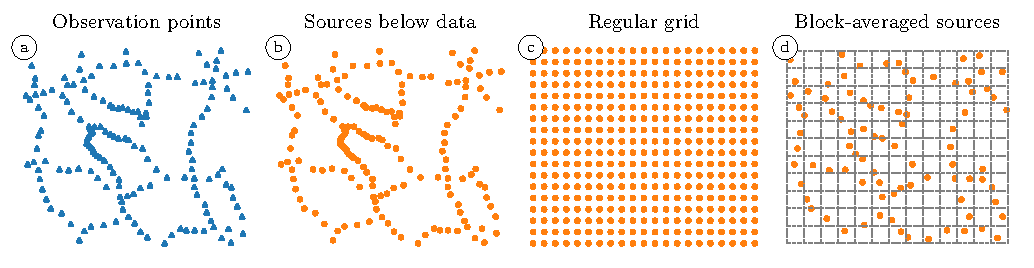
\includegraphics[width=\linewidth]{eql-gradient-boosted/figs/source-layouts-schematics.pdf}
    \caption{
        Sketch of different horizontal layouts for equivalent source models.
        Blue points represent the locations of observations and orange points
        represent the locations of equivalent sources according to different
        layout strategies.
        (a)~Set of \SourceLayoutsSchematicsObservations{} observation points
        that simulate a ground survey.
        (b)~Location of the \SourceLayoutsSchematicsSourceBelowData{} sources
        obtained through the \emph{sources below data} layout.
        (c)~Location of the \SourceLayoutsSchematicsGridSources{} sources
        obtained through the \emph{regular grid} layout.
        (d)~Location of the \SourceLayoutsSchematicsBlockAveragedSources{}
        sources obtained through the \emph{block-averaged sources} layout.
        Grey dashed lines represent the spatial blocks within which the median
        observation location is calculated.
    }
    \label{fig:source_layouts}
\end{figure*}

The most widely used layouts for distributing equivalent sources horizontally
are:

\begin{enumerate}
  \item
    \emph{Sources below data points}: one equivalent source is placed at the
    horizontal location of each data point (Fig.~\ref{fig:source_layouts}b).
    Therefore, the number of sources is equal to the number of observations
    ($M=N$).
  \item
    \emph{Regular grid}: a homogeneous distribution of point sources below the
    survey region (Fig.~\ref{fig:source_layouts}c). A padding region is often
    added to help reduce edge effects. In practice, it often leads to
    underdetermined problems since a large number of sources is required
    ($M>N$).
\end{enumerate}

For ground surveys, the \emph{regular grid} layout needs a sufficiently
small grid spacing to be able to fit the observed data.
This creates an unnecessarily large number of sources in areas where no
observations exist.
In contrast, the \emph{sources below data} layout is more likely to accurately
fit the observed data with many fewer sources, reducing the computational load.
But when applied to airborne surveys, the \emph{sources below data} layout may
place an undesirably large number of sources along the flight paths.
This could lead to aliasing effects on the predicted values, such as the
stripes parallel to flight lines that are often observed when gridding airborne
magnetic data.
The \emph{regular grid} layout can avoid this effect by evenly
distributing sources and using a continuous source layer (e.g.,
right-rectangular prisms or tesseroids).

We propose a new way of distributing equivalent sources horizontally that could
simultaneously reduce the computational load and mitigate some of the drawbacks
of existing layouts.
In the \emph{block-averaged sources} layout,
point sources are placed in the average
position of data points that fall within specified spatial blocks
(Fig.~\ref{fig:source_layouts}d).
This is done by:

\begin{enumerate}
    \item Dividing the survey region into rectangular blocks of equal size.
    \item \label{item:median-position} Computing the median horizontal position
        of the observation points that fall inside each block. Blocks without
        any observation point are omitted.
    \item Assign one point source to each of the median horizontal positions
      calculated in step \ref{item:median-position}.
\end{enumerate}

The number of sources created by this new layout will be less than the number
of observations if the block size is chosen appropriately (i.e., making sure
that blocks are large enough to contain more than a single data point).
The overdetermined problem that arises from this layout has a lower
computational load and is less prone to overfitting the data since the model
complexity is lower.
Moreover, the block averaging process can balance the spacing between sources
along a flight line and between adjacent lines, helping to reduce aliasing
effects in the generated grids.
In Section~\ref{sec:synthetic_distributions}, we demonstrate through tests on
synthetic data that the block-averaged sources layout is able to interpolate
with comparable accuracy to other layouts while using a fraction of the
equivalent sources.


\subsubsection{Depth of sources}

\begin{figure*}[tb!]
    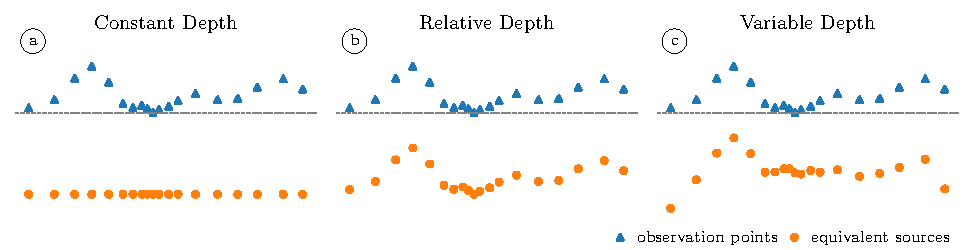
\includegraphics[width=\linewidth]{eql-gradient-boosted/figs/depth_types.pdf}
    \caption{
        Examples of different strategies for assigning depths to equivalent
        sources.
        Here we assign one source for each
        observation point, located at the same horizontal coordinates as the
        data points.
        Source depths are
        (a)~a \emph{constant depth} at a chosen vertical coordinate,
        (b)~a \emph{relative depth} determined by uniformly shifting downward
        the vertical coordinate of data points,
        and
        (c)~a \emph{variable depth} determined by shifting the vertical
        coordinates of the observation points by an amount proportional to the
        average distance to neighbouring sources.
        The distance between data points and their respective sources (a)
        depends on observation height, (b) is constant, and (c) is proportional
        to the horizontal distribution of sources.
        Notice how the closely spaced sources in the middle of the profile (c)
        are shallower than their counterparts in (b).
    }
    \label{fig:depth_types}
\end{figure*}

It is widely known from potential theory that the depth of a point source
influences the wavelength of the observed field at the surface.
This makes the source depth a key parameter affecting the outcome of
interpolation and other operations done with equivalent sources.
Several different strategies for assigning the depths of equivalent sources
have been proposed in the literature.
Here, we will highlight the following (Fig.~\ref{fig:depth_types}):

\begin{enumerate}
  \item
    \emph{Constant depth}:
    The simplest option is to locate all sources at the same depth
    (Fig.~\ref{fig:depth_types}a).
    If the measurements were taken at significantly different altitudes, some
    measurements will be more distant to the sources than others,
    which may create problems for reproducing short wavelengths in high
    altitude points.
 \item
    \emph{Relative depth}:
    The depths of sources are determined by shifting the vertical coordinate of
    data points downward by a fixed amount (Fig.~\ref{fig:depth_types}b).
    The sources will not all be at the same vertical coordinate, but they will
    all be at the same vertical distance from the observation points.
 \item
    \emph{Variable depth}:
    The depths of sources are proportional to the horizontal distance to the
    nearest neighbouring data points or sources (Fig.~\ref{fig:depth_types}c).
    Different variations of this strategy have been proposed before, for
    example \citet{cordell1992}, \citet{guspi2004}, and \citet{Guspi2009}.
    The rationale for this strategy is that if a survey has data points
    clustered in some areas, we may
    want the sources below those areas to be shallower in order to preserve the
    shorter wavelengths that can be measured.
\end{enumerate}

Our approach to the \emph{variable depth} strategy will be:

\begin{equation}
  z = z_{obs} + \Delta z + \alpha h,
  \label{eq:variable_depth}
\end{equation}

\noindent
in which $z$ is the vertical coordinate (positive downwards) of an equivalent
source,
$\Delta z$ is a relative depth shift that is the same for all sources,
$\alpha$ is an dimensionless depth factor,
$h$ is the median horizontal distance to the $k$ nearest neighbouring sources,
and
$z_{obs}$ is a vertical observation coordinate that will depend on the
horizontal layout strategy.
For \emph{sources below data}, it is the vertical coordinate of the data point
corresponding to the given source.
For \emph{regular grid}, it can be interpolated from the vertical coordinates
of all data points.
Finally, for \emph{block-averaged sources} it will be the median vertical
coordinate of the data within the corresponding block.

In Section~\ref{sec:synthetic_distributions}, we test the effectiveness each of
these strategies on synthetic data.

%%%%%%%%%%%%%%%%%%%%%%%%%%%%%%%%%%%%%%%%%%%%%%%%%%%%%%%%%%%%%%%%%%%%%%%%%%%%%%%

\section{Tests on synthetic data}

\begin{figure*}[tb!]
    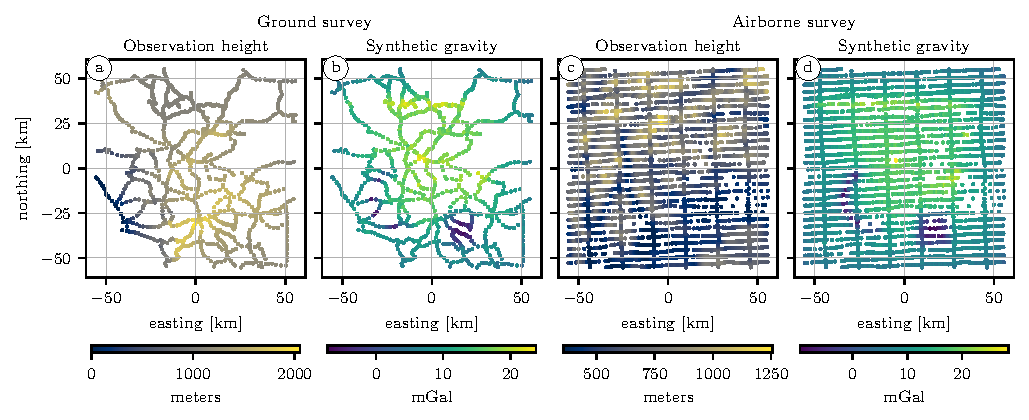
\includegraphics[width=\linewidth]{eql-gradient-boosted/figs/synthetic-survey-layouts.pdf}
    \caption{
        Observation heights and gravity values for the synthetic ground (a-b)
        and airborne (c-d) surveys.
        Heights are given in meters above the zero height plane.
        The synthetic gravity data are contaminated with pseudo-random Gaussian
        noise with zero mean and \SurveyNoise{} standard deviation.
    }
    \label{fig:synthetic-layouts}
\end{figure*}

\begin{figure}[tb!]
    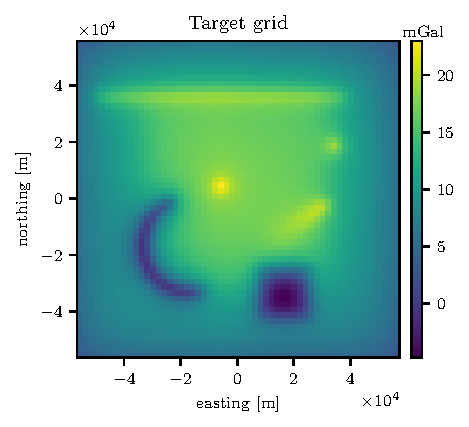
\includegraphics[width=\linewidth]{eql-gradient-boosted/figs/target-grid.pdf}
    \caption{
        Pseudo-color map of the target grid of synthetic gravity data. The grid
        is composed of \TargetEastingSize{}$\times$\TargetNorthingSize{} points
        with a spacing of \TargetSpacing{}. The grid height is \TargetHeight{}
        above the zero height plane.
    }
    \label{fig:synthetic-target}
\end{figure}

We have used synthetic gravity datasets to test the interpolation accuracy of
the difference horizontal and vertical source distribution strategies as well
as the gradient-boosted equivalent sources method.
To generate the data, we created a model of \NPrisms{} right-rectangular
prisms,
distributed in a \ModelEasting{}$\times$\ModelNorthing{} area with depths
varying between \ModelDepth{} and zero.
The density contrast of prisms ranges from \ModelMinDensity{} to
\ModelMaxDensity{}.
The model includes prisms of different shapes, sizes, and depths to create
gravity disturbances with a variety of wavelengths.

We created two synthetic datasets from the model, one simulating a ground
survey and another an airborne acquisition (Fig.~\ref{fig:synthetic-layouts}).
To create the synthetic ground survey, we selected measurement positions from a
portion of a public domain gravity dataset for Southern Africa, available
through the NOAA National Centers for Environmental Information (NCEI).
For the synthetic airborne survey, we used a portion of the Great Britain
Aeromagnetic Survey acquired by Hunting Geology and Geophysics Ltd and Canadian
Aeroservices Ltd between 1955 and 1965 and made publicly available by the
British Geological Survey (BGS).
In both cases, we rescaled the horizontal coordinates of each survey portion to
span an area of \SurveyEasting{}$\times$\SurveyNorthing{}, matching the model
dimensions.
The ground survey contains \GroundSurveyPoints{} observations distributed at
heights between \GroundSurveyMinHeight{} and \GroundSurveyMaxHeight{}
(Fig.~\ref{fig:synthetic-layouts}a).
The airborne survey has \AirborneSurveyPoints{} observations at heights between
\AirborneSurveyMinHeight{} and \AirborneSurveyMaxHeight{}
(Fig.~\ref{fig:synthetic-layouts}c).

The vertical component of the gravitational acceleration generated by the
model was computed  using the method of \citet{nagy2000, nagy2002}
with recent modifications by \citet{fukushima2020},
as implemented in the open-source software Harmonica \citep{harmonica2020}.
We generated a \emph{target grid} of
\TargetEastingSize{}$\times$\TargetNorthingSize{} points with a spacing of
\TargetSpacing{} and located \TargetHeight{} above the zero height plane
(Fig.~\ref{fig:synthetic-target}) to serve as a reference when calculating the
interpolation error.
We then generated synthetic ground (Fig.~\ref{fig:synthetic-layouts}b) and
airborne (Fig.~\ref{fig:synthetic-layouts}d) data to which we added
pseudo-random Gaussian noise with zero mean and \SurveyNoise{} standard
deviation.


\subsection{Source distribution strategies}
\label{sec:synthetic_distributions}

\begin{figure*}[p]
    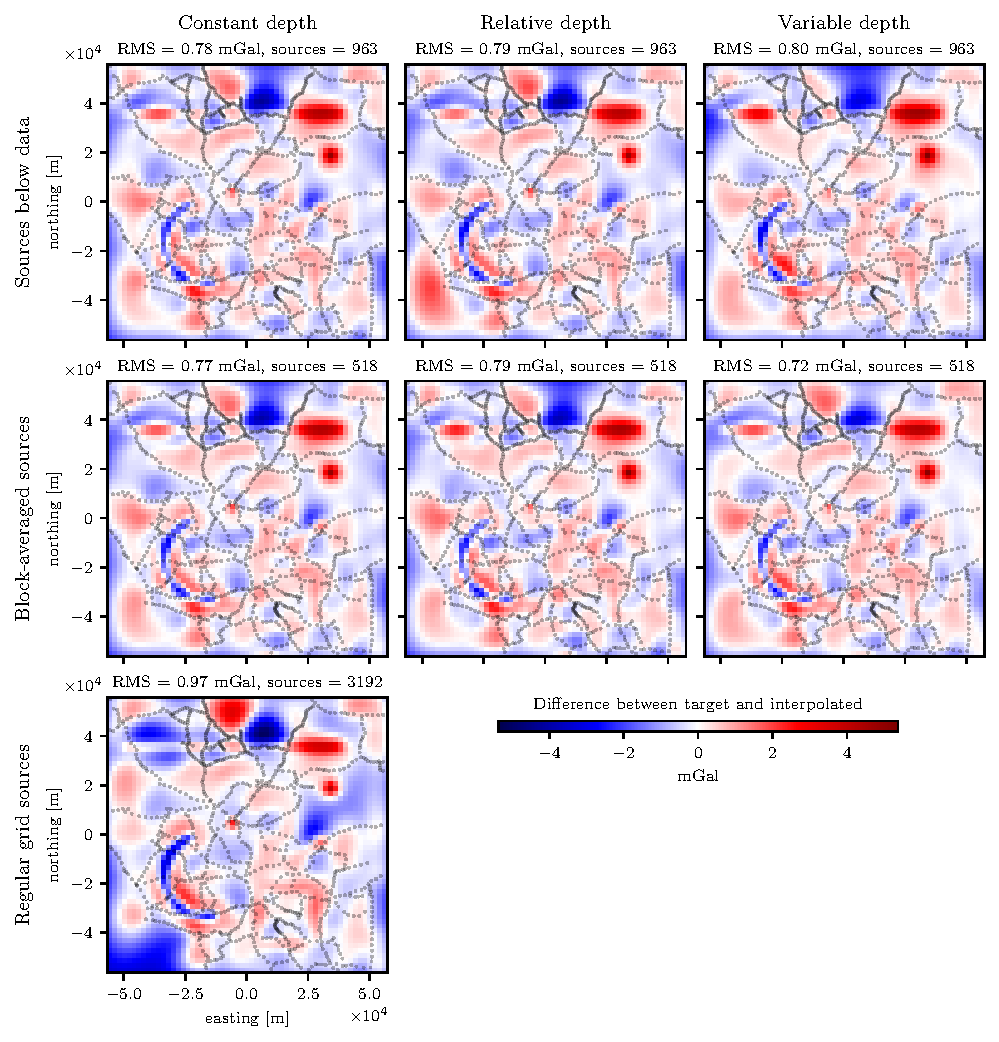
\includegraphics[width=\linewidth]{eql-gradient-boosted/figs/ground_survey_differences.pdf}
    \caption{
        Pseudo-color maps of the differences between the target grid and the
        interpolated synthetic ground survey data produced by each source
        distribution strategy.
        The black dots represent the horizontal location of the synthetic data
        points. The RMS error and total number of equivalent sources is
        reported for each strategy at the top of the respective maps.
    }
    \label{fig:ground-survey-differences}
\end{figure*}

\begin{figure*}[p]
    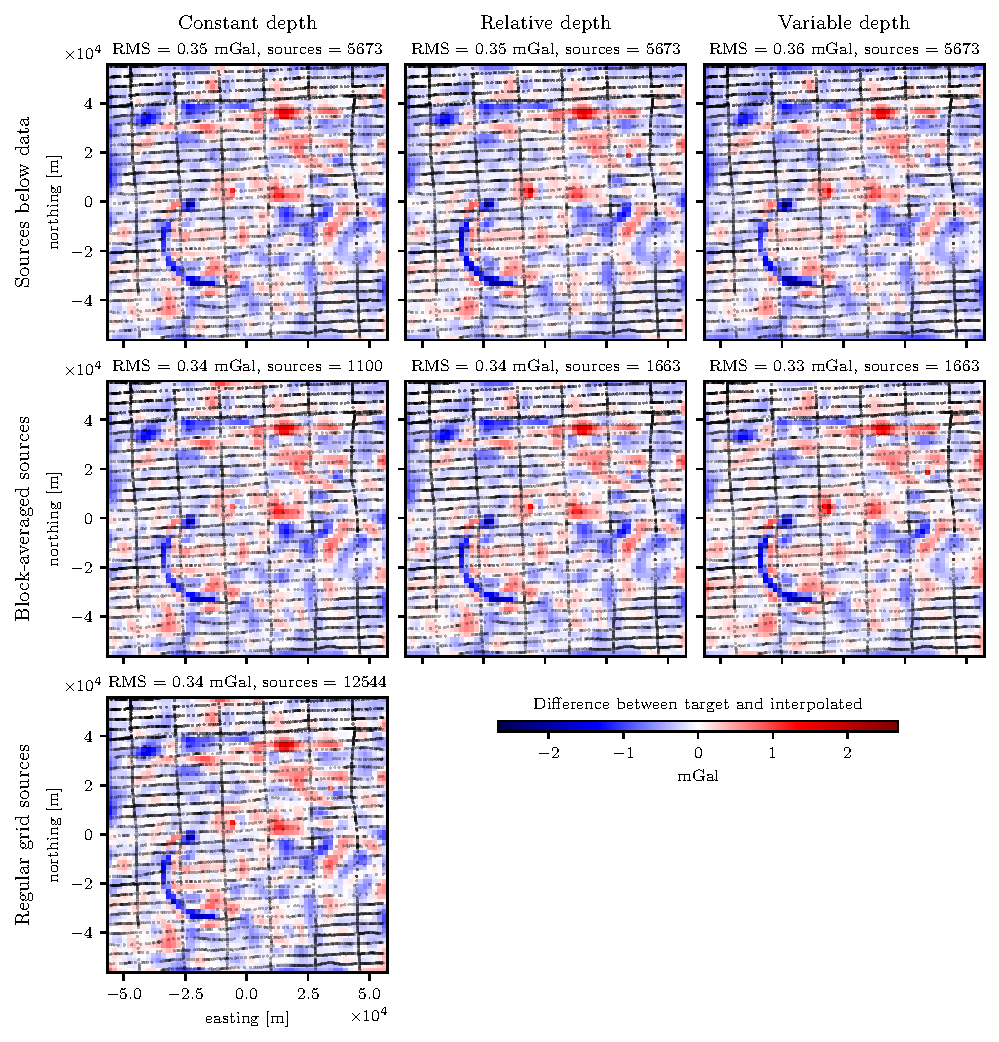
\includegraphics[width=\linewidth]{eql-gradient-boosted/figs/airborne_survey_differences.pdf}
    \caption{
        Pseudo-color maps of the differences between the target grid and the
        interpolated synthetic airborne survey data produced by each source
        distribution strategy.
        The black dots represent the horizontal location of the synthetic data
        points. The RMS error and total number of equivalent sources is
        reported for each strategy at the top of the respective maps.
    }
    \label{fig:airborne-survey-differences}
\end{figure*}

We investigated the effect on interpolation accuracy of different strategies
for distributing the equivalent sources horizontally and vertically.
To do this, we used the damped least-squares solution described in
Section~\ref{sec:eql_inversion} (without gradient boosting) to interpolate the
synthetic datasets (Fig.~\ref{fig:synthetic-layouts}) and compared the results
against the target grid (Fig.~\ref{fig:synthetic-target}).
This process was repeated for each combination of horizontal layout
(\emph{sources below data} and \emph{block-averaged sources}) and depth type
(\emph{constant}, \emph{relative}, and \emph{variable}) and for regular grid
sources with a constant depth, totalling 7 different combinations.

Each source distribution strategy requires certain hyper-parameters to be
chosen in order to build the set of point sources.
For example, using a constant depth needs the definition of the depth and using
block-averaged sources requires the definition of the block size.
The predictive capabilities of the equivalent sources depend on the choice of
these hyper-parameters.
To ensure that our comparisons are fair, we perform an exhaustive search over
combinations of hyper-parameter values (including the damping parameter from
Eq.~\ref{eq:misfit}) to obtain the best prediction that can be achieved by each
source distribution strategy.
Here, the best prediction is defined as the one that minimizes the root
mean-square error (RMS) between interpolated values and the target grid
(Fig.~\ref{fig:synthetic-target}).
The parameter values used in these searches and the one producing the smallest
RMS error are outlined in Tables~\ref{tab:parameters-ground-survey}
and~\ref{tab:parameters-airborne-survey}.

Fig.~\ref{fig:ground-survey-differences}
and~\ref{fig:airborne-survey-differences} show the differences between the
target grid and the best prediction achieved by each source distribution
strategy for the ground and airborne synthetic surveys, respectively.
For the synthetic ground survey, the horizontal layouts produced similar RMS
values of approximately 0.8\mGal{} regardless of the depth type, with the
exception of the regular grid layout which produced a larger RMS of
\BestGroundGridSourcesConstantDepthRms{}\mGal{}.
The differences between the target grid and the interpolated values are larger
in regions of poor data coverage.
Edge effects are present for all strategies but are noticeably smaller for the
combination of block-averaged sources with a variable depth based on the
nearest neighbour distance.
For the synthetic airborne survey, all strategies (including the regular grid)
produced similar RMS errors of approximately 0.3\mGal{}.
The maps of the differences between the target grid and interpolation results
are visually indistinguishable from each other.

%%%%%%%%%%%%%%%%%%%%%%%%%%%%%%%%%%%%%%%%%%%%%%%%%%%%%%%%%%%%%%%%%%%%%%%%%%%%%%%


\subsection{Window size and overlap in gradient boosting}
\label{sec:window_size_and_overlap}

We assessed the trade-offs in interpolation accuracy and computation time of
the gradient-boosted equivalent sources algorithm as a function of the two key
controlling factors: the window size and the amount of overlap between adjacent
windows.
The comparisons were performed against a regular least-squares solution
(Eq.~\ref{eq:least_squares_solution}) using the synthetic airborne data
(Fig.~\ref{fig:synthetic-layouts}c-d).
To avoid biasing the results, we used the same locations of equivalent sources
for both the regular and gradient-boosted interpolations, namely
block-averaged sources with a block size of
\BestAirborneBlockAveragedSourcesRelativeDepthSpacing\m{} and a
relative depth of
\BestAirborneBlockAveragedSourcesRelativeDepthDepth\m{}.

\subsubsection{Window size}
\label{sec:window_size}

The size of the windows controls the size of the Jacobian matrices
$\tilde{\mathbf{A}}_k$ by limiting the number of data points and equivalent
sources used in each step of the gradient-boosting algorithm
(Alg.~\ref{alg:gradient_boosting_window}).
Thus, using smaller windows will reduce the total amount of computer memory
required to estimate the source coefficients.
Nevertheless, smaller windows may produce less accurate interpolations by
failing to achieve the global minimum of the goal function in
Eq.~\ref{eq:misfit}.
The window size might also impact the computation time in non-intuitive ways
since smaller windows generate smaller least-squares problems but also require
more gradient-boosting iterations.

We calculated the interpolation RMS error (between the interpolated grid and
the target grid in Fig.~\ref{fig:synthetic-target}) and computation time for a
fixed window overlap of 50\% and several window sizes.
To avoid any biases introduced by the shuffling of windows, the calculations
were repeated using different seeds for the pseudo-random number generator used
in the shuffling.
Fig.~\ref{fig:gradient-boosted-comparison}a shows the RMS error and
Fig.~\ref{fig:gradient-boosted-comparison}c shows the computation time
required for estimating the source coefficients, both as functions of
the window size.

\begin{figure*}[tb!]
    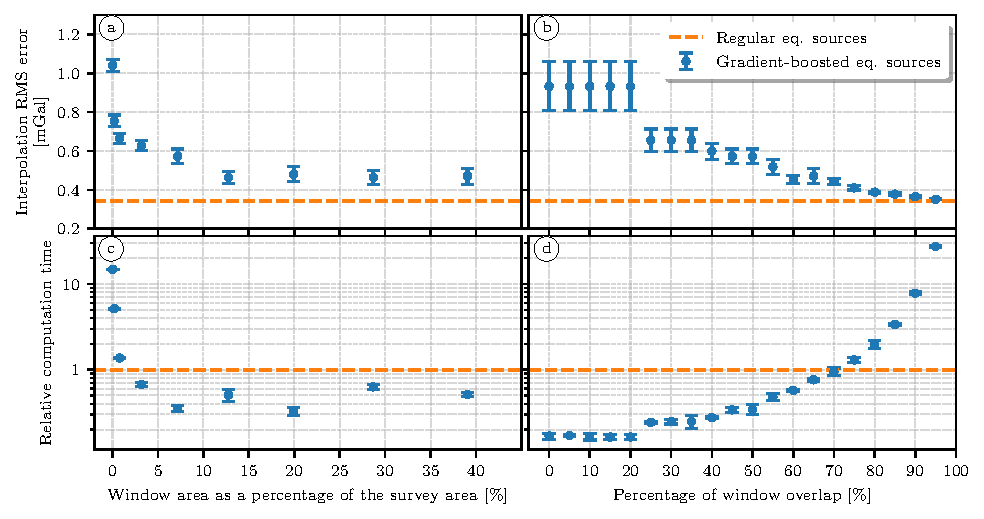
\includegraphics[width=\linewidth]{eql-gradient-boosted/figs/gradient-boosted-comparisons.pdf}
    \caption{
        Interpolation RMS error (a-b) and relative computation time (c-d) for
        regular least-squares equivalent sources (orange dashed lines) and
        gradient-boosted equivalent sources (blue dots and error bars).
        Window overlap is given as a percentage of the window size (an overlap
        of 50\% means that two adjacent windows share an area half of the size
        of the entire window).
        For gradient-boosting, the RMS errors and computation times are the
        means (error bars are 1 standard deviation) of results using different
        seeds for the pseudo-random number generator.
        Computation time is the ratio between the time required to estimate the
        source coefficients for the gradient-boosted and the regular equivalent
        sources.
}
    \label{fig:gradient-boosted-comparison}
\end{figure*}

These results show that the interpolation error for gradient-boosting is
generally larger than the error for regular equivalent sources.
The error decreases asymptotically to within $\sim 40\%$ of the regular
equivalent sources for windows with an area greater than $\sim 10\%$ of the
survey area.
The computation time similarly decreases with window size, with the
gradient-boosting being generally faster than the regular equivalent sources
for windows with an area greater than $\sim 5\%$ of the survey area.
As the window size increases, both RMS error and computation time appear to
stabilize to nearly constant levels.

\subsubsection{Window overlap}

The amount of overlap between adjacent windows plays an important role in the
performance of the gradient-boosted equivalent sources.
It controls the number of iterations and how many times a particular source is
used in the least-squares fitting process.
The experiments in the previous section showed that 50\% overlap was
sufficient to achieve acceptable interpolation accuracy.
However, we studied separately the impacts of the amount of window overlap on
both accuracy and computation time.

We performed a similar experiment to the one in section~\ref{sec:window_size}
but this time kept the window size fixed to \BoostOverlappingWindowSize{} and
varied the amount of overlap from 0\% to 95\% with a step size of 5\%.
All other experimental procedures remained unchanged.
Fig.~\ref{fig:gradient-boosted-comparison}b shows the RMS error and
Fig.~\ref{fig:gradient-boosted-comparison}d shows the computation time
required for estimating the source coefficients, both as functions of
the window overlap.

Our results show that the interpolation RMS error decreases with the amount of
overlap, reaching the same accuracy as the regular equivalent sources at
approximately 90\% overlap.
On the other hand, the computation time increases with the amount of overlap,
becoming larger than that of the regular equivalent sources for overlaps
greater than 70\%.
This is expected since increasing the overlap adds iterations to the gradient
boosting algorithm without decreasing the individual least-squares problem
sizes to compensate.


\subsection{
    Interpolation with gradient boosting
}
\label{sec:gb_interpolation}

Finally, we applied the gradient-boosted equivalent sources to interpolate the
synthetic airborne survey (Fig.~\ref{fig:synthetic-layouts}).
As previously, we used the block-averaged sources layout with a block size of
\EqlBoostAirborneSpacing{}.
Based on the results from section \ref{sec:window_size_and_overlap}, we adopted
a window overlap of 50\% and a window size of \EqlBoostAirborneWindowSize{}.

We estimated the relative depth of the sources and the damping parameter by
comparing the predictions against the values of the target grid.
The search explored \emph{depth} values between \EqlBoostAirborneMinDepth{} and
\EqlBoostAirborneMaxDepth{} and \emph{damping} values between
\EqlBoostAirborneMinDamping{} and \EqlBoostAirborneMaxDamping{} by steps of one
order of magnitude.
The most accurate predictions achieved a RMS error of
\EqlBoostAirborneRmsScore{} with a depth of \EqlBoostAirborneDepth{} and
a damping of \EqlBoostAirborneDamping{}.
It is worth noting that the RMS error achieved by the gradient-boosted
equivalent sources is comparable to the ones obtained by the regular equivalent
sources in Section \ref{sec:synthetic_distributions}.
To highlight the importance of randomizing the order of windows in the
gradient-boosting iterations, we preformed the interpolation once more using
the same values of \emph{damping} and \emph{depth} but this time iterating over
windows in sequential order (South to North, West to East).

\begin{figure}[tb!]
    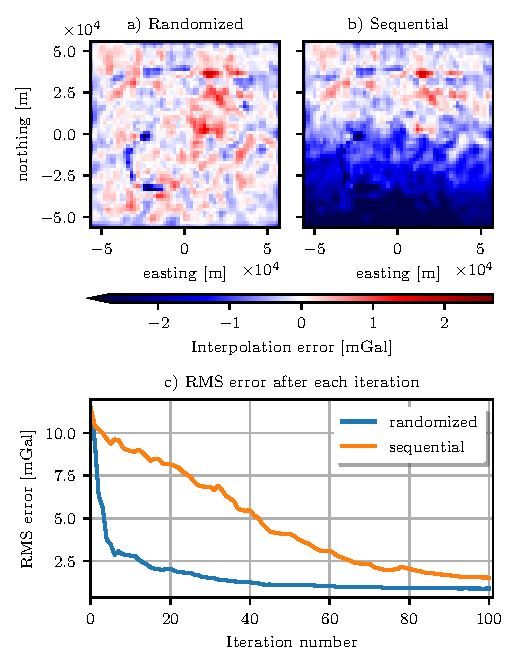
\includegraphics[width=\linewidth]{eql-gradient-boosted/figs/eql-boost-airborne.pdf}
    \caption{
        Interpolation error for gradient-boosted equivalent sources using
        randomized (a) and sequential (b) window order.
        (a and b)~Pseudo-color maps of the differences between the target grid
        and the interpolated synthetic airborne survey data.
        The color scale has been cropped to the same range as
        Fig.~\ref{fig:airborne-survey-differences}.
        (c)~Root-mean squared error after each iteration of the
        gradient-boosting algorithm.
}
\label{fig:eql-boost-airborne}
\end{figure}

Figs.~\ref{fig:eql-boost-airborne}a-b show the differences between the target
grid and the interpolation results for windows in randomized and sequential
order, respectively.
The differences for randomized windows resemble those for regular least-squares
equivalent sources seen in Figs.~\ref{fig:ground-survey-differences} and
\ref{fig:airborne-survey-differences}.
On the other hand, the differences for sequential windows show a clear
trend of large negative differences in the South decreasing towards the North.
This trend is correlated with the order in which windows are executed, with
differences decreasing in absolute value towards the end of the algorithm.
Fig.~\ref{fig:eql-boost-airborne}c shows the RMS error of the fitting process
after each iteration for both window orders, clearly indicating that
a randomized window order leads to faster convergence of the algorithm.


%%%%%%%%%%%%%%%%%%%%%%%%%%%%%%%%%%%%%%%%%%%%%%%%%%%%%%%%%%%%%%%%%%%%%%%%%%%%%%%

\section{Gridding gravity data from Australia}

\begin{figure*}[p]
    \includegraphics[width=\linewidth]{eql-gradient-boosted/figs/australia.png}
    \caption{
      Pseudo-color maps of observed (a and c) and
      interpolated (b and d) gravity disturbance of Australia.
      The observed values in a and c are plotted as colored circles.
      The red rectangle marks the boundaries of the highlight maps in c
      and d.
      Observations are part of a compilation by \citet{wynne2018} of
      over 1.7 million ground gravity measurements.
      Interpolated values were obtained through gradient-boosted equivalent
      sources and calculated on a regular grid at \AustraliaEqlGridHeight{}
      over the WGS84 ellipsoid.
    }
    \label{fig:australia}
\end{figure*}

This section will demonstrate how gradient-boosted equivalent sources can be
used to interpolate large datasets onto regular grids at uniform height.
For this purpose, we selected an open-access compilation of ground gravity
surveys over Australia made by \citet{wynne2018} and filtered and referenced to
the WGS84 ellipsoid by \citet{australia_compilation}.
It contains over 1.7 million data points and covers most of the Australian
territory at variable point spacings.
Our goal is to create a 1~arc-minute resolution grid of gravity disturbances at
a constant geometric height of \AustraliaEqlGridHeight{} (the largest height of
observations).

We computed the gravity disturbance by removing the normal gravity of
the WGS84 ellipsoid from the observed gravity data (Fig.~\ref{fig:australia}).
Here, normal gravity was computed at each observation point through the
closed-form formula of \citet{ligotze2001} using the Boule software
\citep{boule2020}.
Finally, we converted the observations to planar Cartesian coordinates by
applying a Mercator projection.

We start the interpolation process by defining a set of block-averaged sources
using a block size of 1.8\km{}, resulting in a total of
\AustraliaEqlNSources{}~point sources.
The block size was chosen to match the desired resolution of the final grid
(1~arc-minute is approximately 1.8\km{} at the equator).
Based on the results obtained in Section~\ref{sec:synthetic_distributions}, we
have chosen to use the \emph{relative depth} strategy.
The window overlap was once again fixed at 50\%.
To determine the size of the windows, we calculated the amount of computer memory
needed to store the largest Jacobian matrix for different values of window size
(Fig.~\ref{fig:australia-memory-cv-error}a).
We have chosen a size of \AustraliaEqlWindowSize{} in order to limit the
amount of memory needed to under 16~Gigabytes.

\begin{figure}[tbh!]
    \makeatletter%
    \if@twocolumn%
        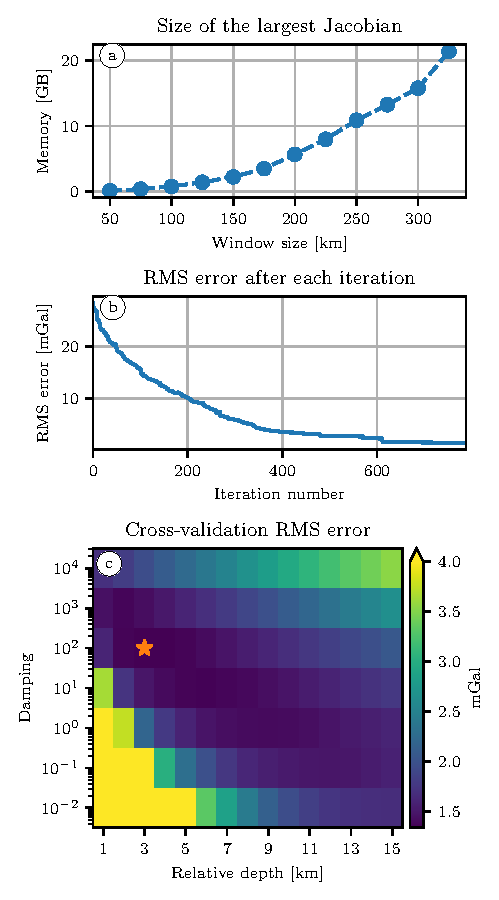
\includegraphics[width=\linewidth]{eql-gradient-boosted/figs/australia-memory-cv-error.pdf}
    \else% \@twocolumnfalse
        \centering
        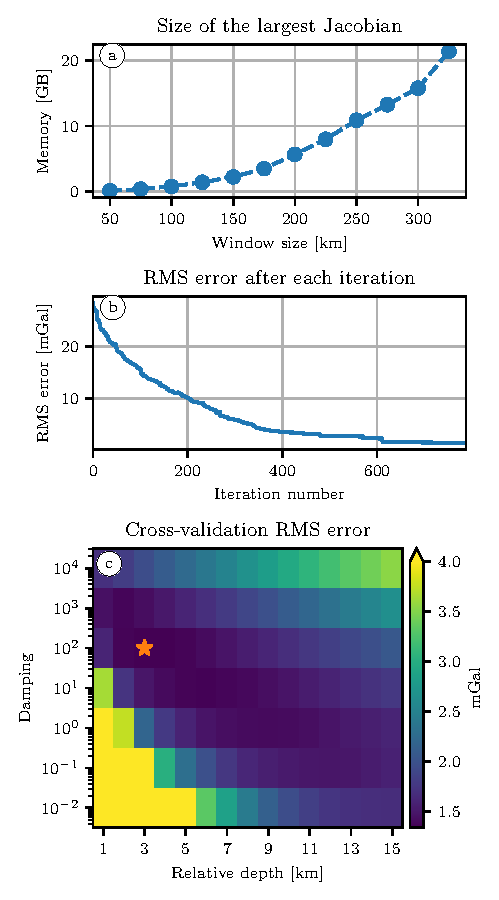
\includegraphics[width=0.6\linewidth]{eql-gradient-boosted/figs/australia-memory-cv-error.pdf}
    \fi
    \makeatother
    \caption{
        (a) Amount of computer memory needed to store the largest Jacobian
        matrix for different window sizes. Our implementation uses double
        precision floating point numbers (64 bits) for the Jacobian.
        (b) Root-mean square error against the observed data after each
        iteration of the gradient-boosting algorithm.
        (c) K-Fold cross-validation root-mean square errors obtained for each
        pair of damping and depth parameters. The orange star highlights the
        minimum.
    }
    \label{fig:australia-memory-cv-error}
\end{figure}

We determined the depth of the sources and the damping parameter by applying
K-Fold cross-validation through the scikit-learn library \citep{sklearn2011}.
The method randomly divides the original data into $k$ sets (folds), fits the
model using only data from $k - 1$ folds, and validates the model by comparing
its predictions against the one remaining fold.
This process is carried out once for each one of the $k$ folds, leading to
an estimated mean cross-validation RMS error for the model.
To speed up the computation, we only performed the cross-validation on a subset
of the data corresponding to an area of
\AustraliaSmallAreaEastingSize{}$\times$\AustraliaSmallAreaNorthingSize{}
containing \AustraliaSmallAreaNPoints{} points.
We ran the cross-validation repeatedly for combinations of \emph{depth},
ranging from \AustraliaDepthMin{} to \AustraliaDepthMax{},
and \emph{damping}, from \AustraliaDampingMin{} to \AustraliaDampingMax{} in
steps of one order of magnitude.
Figure \ref{fig:australia-memory-cv-error}c shows the resulting
cross-validation RMS errors and highlights the minimum value of
\AustraliaEqlRmsScore{}, which corresponds to a relative depth of
\AustraliaEqlDepth{} and a damping equal to \AustraliaEqlDamping{}.

Finally, we proceeded to estimate the source coefficients using the entire
dataset and the parameters previously determined.
The estimated source coefficients were then used to predict the values of the
gravity disturbance on a regular grid of
\AustraliaEqlGridNLongitude{}$\times$\AustraliaEqlGridNLatitude{} points at
\AustraliaEqlGridHeight{} above the ellipsoid.
On a modest workstation with 16 cores and 16~Gigabytes of RAM,
estimating the \AustraliaEqlNSources{} coefficients with gradient-boosting took
$\sim 1.3$~hours and the prediction step took $\sim 18$~minutes.

Fig.~\ref{fig:australia} shows the original data distribution and the
interpolated grid.
Grid points that are further than 50\km{} from the nearest data point are
masked to avoid unrealistic extrapolations.
Fig.~\ref{fig:australia-memory-cv-error}b shows the RMS error against the
observed data after each iteration of the algorithm.
Fig.~\ref{fig:australia-residuals} shows the difference between the observed
and predicted gravity disturbances.
The inset figure shows a histogram of these residuals, which are approximately
normally distributed around zero.

\begin{figure}[tb!]
    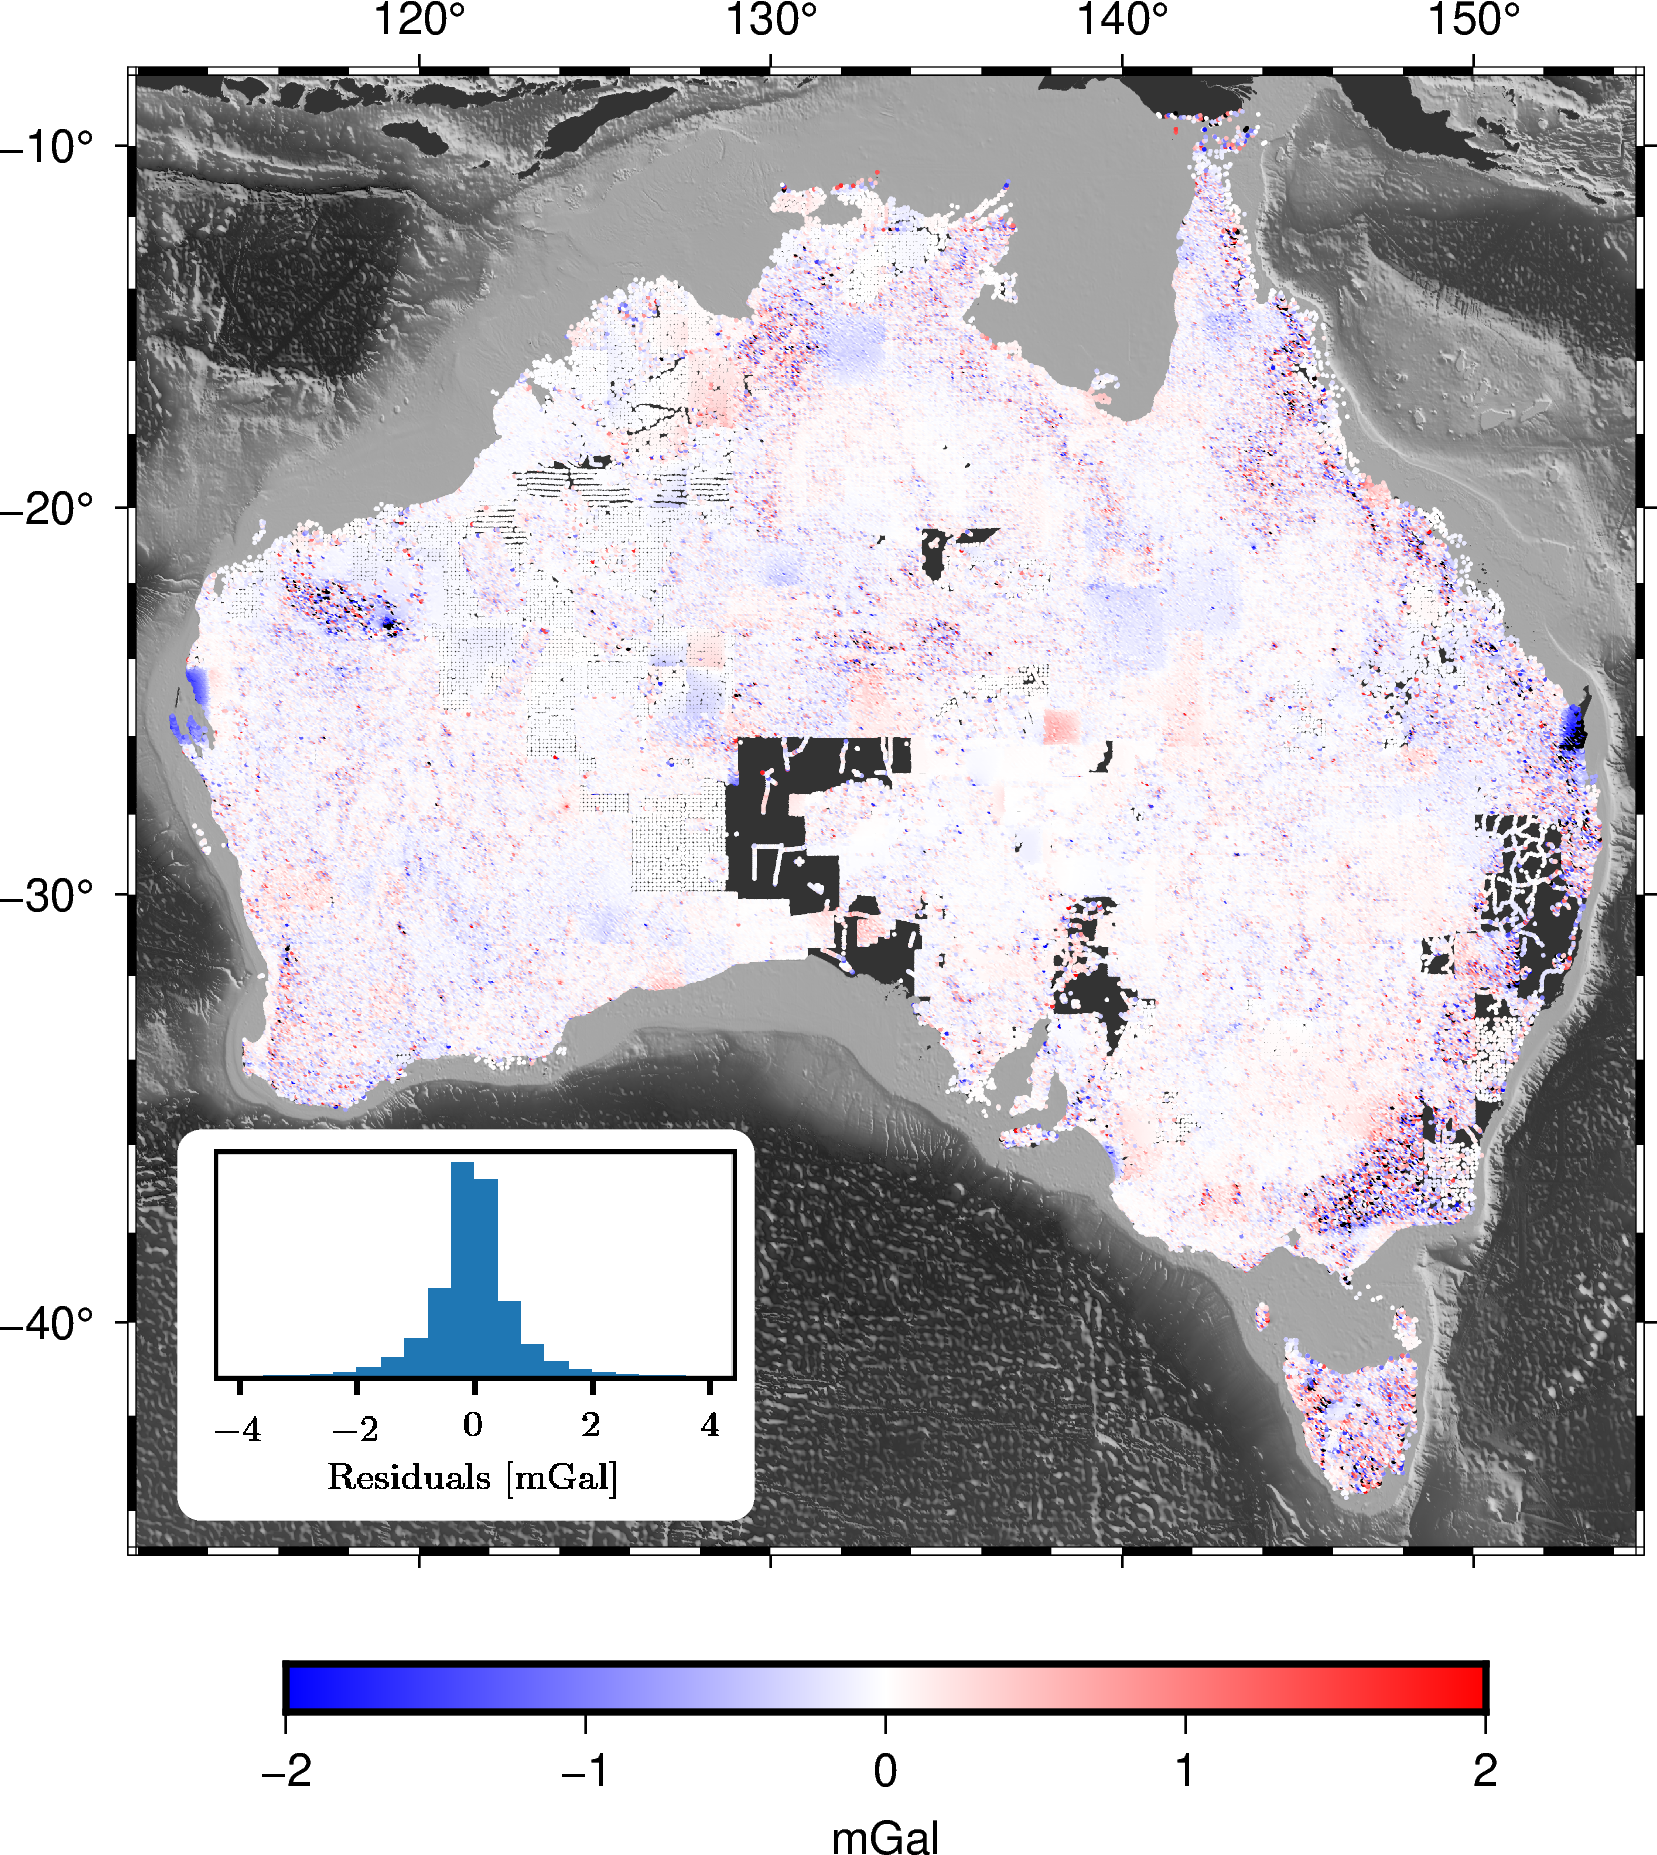
\includegraphics[width=\linewidth]{eql-gradient-boosted/figs/australia-residuals.png}
    \caption{
        Residuals. Differences between the gravity disturbance data from
        Australia and the predicted values by the estimated equivalent sources
        on the same observation points. The color map has been truncated to
        improve the visualization around the largest portion of residual
        values. The inset plot shows a histogram of the residuals.
    }
    \label{fig:australia-residuals}
\end{figure}


%%%%%%%%%%%%%%%%%%%%%%%%%%%%%%%%%%%%%%%%%%%%%%%%%%%%%%%%%%%%%%%%%%%%%%%%%%%%%%%

\section{Discussion}

\subsection{Location of sources}

The results of our tests on synthetic data
(Figs.~\ref{fig:ground-survey-differences}
and~\ref{fig:airborne-survey-differences}) show that there are no significant
differences in interpolation accuracy between source distribution strategies,
both in terms of the interpolation RMS errors and from visual inspection of the
difference maps.
Therefore, we conclude that all source distribution strategies are able to
produce comparable interpolations.
Nevertheless, the \emph{block-averaged sources} strategy makes use of fewer
sources when compared with other strategies, which reduces the computational
load of estimating the sources coefficients and forward modelling.
To ensure that the interpolation is able to reproduce the high frequencies in
the data, the block size used in the averaging should be chosen to match the
desired grid resolution.

The choice of source depth strategy does not appear to significantly impact the
interpolation RMS error.
In the particular case of a sparse ground survey with block-averaged sources,
the use of a variable depth visibly reduced edge effects and artifacts in areas
of poor data coverage.
At a first glance, the choice of a depth strategy would not seem to impact
the computation time.
However, when searching for the set of hyper-parameters that produce the most
accurate interpolation (e.g., through cross-validation), one must solve the
inverse problem once for every possible combination of parameters.
A depth strategy like the \emph{variable depth} requires a higher number of
hyper-parameters (depth shift $\Delta z$, depth factor $\alpha$, and the number
of nearest neighbours $k$ from Eq.~\ref{eq:variable_depth}) than other
strategies which only require a single parameter.
Having more parameters means increasing the dimensions of the parameter space
and thus increasing the number of possible combinations.
Thus, we recommend using a \emph{constant depth} or a \emph{relative depth}
when processing large datasets in order to minimize computation time.

\subsection{Gradient boosting}

From Fig.~\ref{fig:gradient-boosted-comparison}a
and~\ref{fig:gradient-boosted-comparison}c, we can see that the
gradient-boosted equivalent sources produce slightly less accurate
interpolation results but are able to achieve smaller computation times than
regular equivalent sources.
The reduction of the accuracy might be due to the gradient boosting algorithm
failing to converge to the global minimum of the goal function.
As the windows increase in size, interpolation error decreases because more data
points are included into the least-squares fitting of the source coefficients.
At the same time, the fitting process becomes faster because of a reduction in
the number of iterations.
Our results indicate that it is desirable to maximize the window size,
which can be done up to the point that the Jacobian matrices still fit within
the available computer memory.

The results shown in Figs.~\ref{fig:gradient-boosted-comparison}b
and~\ref{fig:gradient-boosted-comparison}d indicate that using
window overlap values between 40\% and 70\% strike a balance between
accuracy and computation time.
This corroborates our initial choice of 50\% overlap, which is good enough for
producing accurate predictions in reasonable times.

Finally, the results in Fig.~\ref{fig:eql-boost-airborne} highlight the
importance of randomizing the order in which the overlapping windows are
iterated.
Running the gradient boosting algorithm sequentially produces less accurate
predictions and decreases the convergence rate of the method.

\subsection{Australia gravity data}

The application of the gradient-boosted equivalent sources to the Australian
gravity dataset demonstrates that the method is able to interpolate and
upward-continue large datasets in a reasonable amount of time using only modest
computational resources.
The resulting grid (Fig.~\ref{fig:australia}) preserves the high resolution of
the original data while avoiding aliasing artifacts due to the block averaging
of the source locations.
Some parts of the grid are smoother and have lower amplitudes than the original
data (e.g., some southwestern parts), which is expected from the upward
continuation that was performed to have the grid at a constant height.
From the cross-validation analysis on a subset of the data, we estimate that
the interpolation error is approximately \AustraliaEqlRmsScore{}.

The largest residuals in Fig.~\ref{fig:australia-residuals} are located in
regions with high-amplitude short-wavelength features in the observed data.
This is expected since the method involves some degree of smoothing because of
the use of damping and the source depths.
There are also low-amplitude long-wavelength residual signals that seem to
coincide with some of the windows of the gradient-boosting method.
A possible cause of these features is inability of the equivalent-sources
within a window to adequately fit the long-wavelength components of the data.
We note, however, that all of these long-wavelength residuals are smaller than
1\mGal{} in amplitude and do not represent a significant source of errors.

The elongated valley around the minimum of the cross-validation RMS errors
(Fig.~\ref{fig:australia-memory-cv-error}c) shows that there is ambiguity in
the choice of damping and source depths.
One could choose a large damping with a small depth or a small damping with a
large depth to achieve roughly the same interpolation result.
This is expected since both parameters control the smoothness of the
interpolation.

%%%%%%%%%%%%%%%%%%%%%%%%%%%%%%%%%%%%%%%%%%%%%%%%%%%%%%%%%%%%%%%%%%%%%%%%%%%%%%%

\section{Conclusions}

The equivalent source technique has been proven to be well suited for
interpolating gravity disturbances and magnetic anomalies.
The two main reasons that make it to stand out from other 2D interpolation
methods is the fact that the equivalent sources take into account the height of
the observations and that the interpolated values will always be harmonic
functions.
The main challenge of using equivalent sources in practice is the high
computational load of estimating the coefficients of the equivalent sources,
specially the computer memory needed to store the Jacobian matrix.

We present two strategies that could be simultaneously applied to interpolate
datasets with millions of points on modest hardware:
block-averaging source locations, which reduces the number of equivalent
sources needed for the interpolation,
and the gradient-boosted equivalent source algorithm, which breaks down the
inverse problem into smaller sets of equivalent sources defined by overlapping
windows.
Both methods were tested against synthetic datasets in order to compare their
accuracy and how they perform in terms of computational efficiency.

Our results show that the block-averaged sources reduce the computational
load needed to estimate source coefficients in comparison to two traditional
strategies (placing sources below data points or on regular grids).
We also show that this reduction of the number of sources does not affect
the accuracy of the predictions.
The use of block-averaged sources may also prevent aliasing of the interpolated
values, specially when the observations are unevenly sampled (e.g., airborne
and shipborne surveys).
Special attention must be payed when choosing the size of the blocks for
averaging.
As a thumb rule, we recommend choosing a size approximately equal to
the resolution of the regular grid where the values will be interpolated.

Tests that compared strategies for the vertical location of the
sources showed that any one of the three strategies tested
(\emph{constant depth}, \emph{relative depth} and \emph{variable depth})
produces comparable accuracy of interpolation.
Nevertheless, we are more prone to recommending either the \emph{constant
depth} or the \emph{relative depth} for most applications because they involve
less hyper-parameters that would need to be configured before the actual
interpolation.

Gradient-boosted equivalent sources were shown to heavily reduce the computer
memory needed to estimate source coefficients, making it possible to
interpolate large datasets with millions of points that would otherwise produce
Jacobian matrices larger than the available memory.
The interpolations obtained though this new method achieve close to the same
accuracy than the regular equivalent sources, while reducing the computation
time by approximately a factor of three.
We also show that an overlap of 50\% between adjacent windows achieves a good
compromise between accuracy and computation time.
The size of the overlapping windows should be chosen as the maximum value
possible that creates Jacobian matrices that still fit into computer memory.
Moreover, randomizing the order in which the windows are iterated increases the
convergence rate of the algorithm and is essential to producing accurate
predictions.

The gradient-boosting method can be used in conjunction with any horizontal
source layout, depth strategy, or source type (e.g., point sources, prisms,
tesseroids) because it does not rely on assumptions about the sources.
Future research should investigate the application of gradient boosting to
other equivalent source methods.

%%%%%%%%%%%%%%%%%%%%%%%%%%%%%%%%%%%%%%%%%%%%%%%%%%%%%%%%%%%%%%%%%%%%%%%%%%%%%%%

\section*{Data and code availability}

The Python source code used to produce all results and figures presented here
is available at
\url{https://doi.org/10.6084/m9.figshare.13604360} and
\url{https://github.com/compgeolab/eql-gradient-boosted}
under the BSD 3-clause open-source license.

The gradient-boosted equivalent sources implementation is based on the
equivalent source code in the Harmonica library \citep{harmonica2020}.
Other software used in this study includes:
Pooch \citep{pooch2020} for downloading and caching datasets,
Verde \citep{verde2018} for block reductions and coordinate manipulations,
Boule \citep{boule2020} for normal gravity calculations,
xarray \citep{xarray2017} and Numpy \citep{numpy} for handling
multidimensional arrays and numerical computations,
Numba \citep{numba2015} for just-in-time compilation and parallelization,
scikit-learn \citep{sklearn2011} for cross-validation,
Matplotlib \citep{Hunter2007} and PyGMT \citep{pygmt2020} for generating
the figures and maps,
and the Jupyter notebook programming environment \citep{jupyter2016}.
Harmonica, Boule, Pooch, and Verde are part of the Fatiando a Terra project
\citep{Uieda2013}.

All datasets used are open-access and publicly available.
The synthetic surveys were generated using
a public domain gravity dataset for Southern Africa distributed by the
NOAA NCEI (\url{https://www.ngdc.noaa.gov/mgg/gravity/gravity.html})
and the Great Britain Aeromagnetic
Survey distributed by the
British Geological Survey (BGS) under an Open Government License
(\url{https://www.bgs.ac.uk/products/geophysics/aeromagneticRegional.html}).
The shaded relief in Fig.~\ref{fig:australia} is the SRTM15+ dataset by
\citet{tozer2019}.
The Australian ground gravity
data is based on a compilation distributed by Geoscience Australia under a
Creative Commons Attribution 4.0 International Licence \citep{wynne2018}  which
was filtered and referenced to the WGS84 ellipsoid by
\citet{australia_compilation} and is distributed under the same license
(\url{https://doi.org/10.6084/m9.figshare.13643837}).


%%%%%%%%%%%%%%%%%%%%%%%%%%%%%%%%%%%%%%%%%%%%%%%%%%%%%%%%%%%%%%%%%%%%%%%%%%%%%%%

\section*{Acknowledgements}

We are indebted to the developers and maintainers of the open-source software
without which this work would not have been possible.
We would also like to thank Editor Frederik Simons, Assistant Editor Fern
Storey, and two anonymous reviewers for their constructive comments.
S.R. Soler is supported by a scholarship from CONICET, Argentina.
This work contains British Geological Survey materials ©~UKRI.
S.R. Soler and L. Uieda jointly developed the initial idea, analysed the
results, and wrote the paper. S.R. Soler produced all results and developed the
software implementation with the assistance of L. Uieda.

\endgroup

%==============================================================================
\chapter{Dual-layer magnetic equivalent sources}

\begingroup
%%%%%%%%%%%%%%%%%%%%%%%%%%%%%%%%%%%%%%%%%%%%%%%%%%%%%%%%%%%%%%%%%%%%%%%%%%%%%%%
% Set variables with the title, authors, etc.
\newcommand{\Title}{Transforming Total Field Anomaly into Anomalous Magnetic Field: Using Dual-Layer Gradient-Boosted Equivalent Sources}
\newcommand{\TitleShort}{Magnetic Dual-Layer Gradient-Boosted Equivalent Sources}

\newcommand{\Year}{2025}
\newcommand{\SubmittedOn}{2025/04/11}
\newcommand{\PublishedOn}{2024/09/01}

\newcommand{\AuthorShort}{Uppal \textit{et al.}}
\newcommand{\Authors}{%
  India Uppal\textsuperscript{1},
  Leonardo Uieda\textsuperscript{2},
  Vanderlei Coelho Oliveira Jr.\textsuperscript{3},
  Richard Holme\textsuperscript{1}
}
\newcommand{\Email}{I.Uppal@liverpool.ac.uk}
\newcommand{\Corresponding}{%
  Corresponding author: India Uppal <\href{mailto:\Email}{\Email}>
}
\newcommand{\Affiliations}{%
  \textsuperscript{1} University of Liverpool, UK;
  \textsuperscript{2} Universidade de São Paulo, Brazil;
  \textsuperscript{3} Observatório Nacional, Brazil;
}
\newcommand{\AuthorORCIDs}{%
  IU (\href{https://orcid.org/0000-0003-3531-2656}{0000-0003-3531-2656});
  LU (\href{https://orcid.org/0000-0001-6123-9515}{0000-0001-6123-9515});
  VCOJr (\href{https://orcid.org/0000-0002-6338-4086}{0000-0002-6338-4086});
  RH (\href{https://orcid.org/0009-0002-2178-2083}{0009-0002-2178-2083});
}

\newcommand{\Journal}{Geophysical Journal International}
\newcommand{\JournalDOI}{YYYYY/YYYYYYY}
\newcommand{\PreprintDOI}{XXXXX/XXXXXXX}
\newcommand{\ArchiveDOI}{10.5281/zenodo.15120458}
\newcommand{\GitHubRepository}{compgeolab/eqs-gb-norm-of-b}

\newcommand{\Keywords}{%
  Magnetic anomalies: modelling and interpretation;
  Inverse theory;
  Antarctica;
}


\begin{summarybox}
    \noindent
    This chapter was originally developed as
    \textbf{``Uppal, I., Uieda, L., Oliveira Jr., V. C. and Holme, R. (\Year).
    \Title{}.''} and has not yet been published.
    It is published here under the terms of the CC-BY license.
    A version of this text can be found in
    \url{https://github.com/\GitHubRepository}.
\end{summarybox}

\section*{Abstract}
Potential field data often require interpolation onto a regular grid at constant height before further analysis. A widely used approach for this is the equivalent sources technique, which has been adapted over time to improve its computational efficiency and accuracy of the predictions. However, many of these approaches still face challenges, including border effects in the predictions or reliance on a stabilising parameter. To address these limitations, we introduce the dual-layer gradient-boosted equivalent sources to: (1) use a dual-layer approach to improve the predictions of both short- and long-wavelength signals, as well as, reduce border effect; (2) use block-averaging and the gradient-boosted equivalent sources method to reduce the computational load; (3) apply block K-Fold cross-validation to guide optimal parameter selection for the model. The proposed method was tested on both synthetic datasets and the ICEGRAV aeromagnetic dataset to evaluate the methods ability to interpolate and upward continue onto a regular grid at constant height, as well as predict the amplitude of the anomalous field from total-field anomaly data. The dual-layer approach proved better compared to the single-layer approach when predicting both short- and long-wavelength signals, particularly in the presence of truncated long-wavelength anomalies. The use of block-averaging and the gradient-boosting method improve the dual-layer approach computationally efficiency, being able to grid over 400,000 data points in under 2 minutes on a moderate workstation computer.

% %%%%%%%%%%%%%%%%%%%%%%%%%%%%%%%%%%%%%%%%%%%%%%%%%%%%%%%%%%%%%%%%%%%%%%%%%%%%%%%

\section{Introduction}

Potential field data often need to be interpolated onto a regular grid at constant height before further application, such as modelling crustal structures and geological interpretation. However, many gridding methods do not consider the variable survey heights which are typical of airborne data. Additionally, most methods do not take advantage of the fact that potential fields are harmonic functions. For example, the total field magnetic anomaly is harmonic when the magnitude of the anomalous field is much smaller than the magnitude of the geomagnetic field, which is true for most instances in which the total field anomaly is observed \citep{Blakley1995}.

A widely used approach that addresses these issues is the equivalent sources
(also known as equivalent layer) technique, first introduced by
\citet{dampney1969} and based on potential theory \citep{Kellogg1967}. This
method approximates any harmonic function as the sum of discrete point source
effects, which are then used to predict the potential field in unobserved
locations. However, estimating the source coefficients that best fit the
observed data is computationally demanding and inherently non-unique. Since its
introduction, numerous adaptations of the EQS Technique have been developed to
improve the computational efficiency and accuracy, such as: \citet{Leao1989},
\citet{cordell1992}, \citet{Mendona1994}, \citet{Guspi2009}, \citet{Li2010},
\citet{OliveiraJr2013}, \citet{Siqueira2017}, \citet{Jirigalatu2019},
\citet{Mendona2020}, \citet{Li2020}, \citet{Soler2021}, \citet{Takahashi2022}
and \citet{Piauilino2024}. A comprehensive review of the equivalent sources
technique was undertaken by \citet{OliveiraJr2023} and we refer readers to it
for more information.

For magnetic data in particular, the recent study of \citet{Li2020} identified that incorporating an additional deeper layer of equivalent sources improved the accuracy of the predictions, particularly for the long-wavelength components. \citet{Li2020} fit both shallow and deep equivalent source layers to the observed data simultaneously using prisms as the sources. This required a depth-weighing factor to prevent the shallow layer coefficients from dominating, due to the sensitivity matrix elements of the shallow layer being much larger than those associated with the deep layer.Fitting both layers at once also significantly increases the computational cost of the inversion.

A strong motivation for accepting such a cost is the ability to calculate the amplitude of the anomalous magnetic field from the total-field anomaly observations. The anomalous field is the magnetic field produced by crustal sources and the total-field anomaly is approximately the projection of this field onto the direction of the geomagnetic field \citep{Blakley1995}. Although 3D non-linear inversions of total-field anomaly are known to be sensitive to the often unknown magnetisation direction, \citet{HidalgoGato2021} show that inversion of the amplitude of the anomalous magnetic field are much less sensitive to uncertainty in the magnetisation direction. Additionally, \citet{Melo2021} demonstrates the amplitude of the anomalous field can be useful for interpreting magnetic data at low latitudes, where other techniques, such as reduction-to-the-pole, tend to be unstable.

A caveat of using the equivalent sources techniques is the need for manual selection of hyper-parameters, such as the damping regularisation parameter and the depth of the equivalent sources. A widely used machine learning technique, often used in statistics, for assessing how well a model is at making predictions is cross-validation (CV). \citet{Geisser1975} introduced the K-Fold method to reduce computational load compared to other cross-validation methods.
In equivalent sources processing, \citet{Soler2021} applied K-Fold cross-validation to estimate the damping parameter and the depth of the equivalent sources when gridding gravity data over the country of Australia. However, \citet{Roberts2017} later showed that when observations are spatially auto-correlated, meaning that nearby observations have similar values, a common feature of potential-field data due to their smooth nature, K-Fold cross-validation tends to underestimate the interpolation error and leads to overfitting of the model. To combat this, \citet{Roberts2017} developed the Blocked K-Fold method, specifically designed for cross-validation of spatially auto-correlated data.

This study presents the dual-layer gradient-boosted magnetic equivalent sources method to fit total field anomaly data and predict the norm of the anomalous magnetic anomalous field. This creates a dataset less dependent on the direction of Earth’s main field and crustal magnetisation.
The approach mitigates the computational challenges of applying a dual layer approach to millions of data points and reduces border effects. This enhances both the efficiency and the accuracy by:

\begin{enumerate}
  \item Fitting a deep equivalent source layer of magnetic dipoles to a reduced set of observed data by block-averaging the data before inversion.
  \item Fitting a second, shallower layer of equivalent sources to the residuals from the deep equivalent sources using the gradient-boosting method of \citet{Soler2021}.
  \item Composing the final prediction of either total-field anomaly or norm of the anomalous field by the summation of the predictions from both layers on a regular grid.
  \item Using Block K-Fold cross-validation to assist in the determination the optimal damping parameter and depth of the equivalent sources.
\end{enumerate}

\noindent
This approach demonstrates the effectiveness of the dual-layer method on synthetic data and a real aeromagnetic survey from Antarctica.


%%%%%%%%%%%%%%%%%%%%%%%%%%%%%%%%%%%%%%%%%%%%%%%%%%%%%%%%%%%%%%%%%%%%%%%%%%%%%%%
\section{Methodology}

The observed total field anomaly ($\Delta T$) is the difference between the measured norm of the total magnetic field ($\vec{\mathbf{T}}$) and the norm of the regional reference field ($\vec{\mathbf{F}}$), usually represented by the International Geomagnetic Reference Field (IGRF), at the time of measurement:
\begin{equation}
    \Delta T = \vert \vec{\mathbf{T}} \vert - \vert \vec{\mathbf{F}} \vert
    \ .
\end{equation}

\noindent
The total magnetic field ($\vec{\mathbf{T}}$) is the sum of the anomalous magnetic field vector ($\vec{\mathbf{B}}$) and the regional field vector ($\vec{\mathbf{F}}$) \citep{Blakley1995, Langel1998, Oliveira2015Estimation}. The total field anomaly ($\Delta T$) can therefore be given by
\begin{equation}
    \Delta T = \vert \vec{\mathbf{F}} + \vec{\mathbf{B}} \vert - \vert \vec{\mathbf{F}} \vert
    \ .
\end{equation}
\noindent
For the majority of crustal anomalies measured by airborne and shipborne surveys, $\vec{\mathbf{B}}$ is much smaller in magnitude compared to $\vec{\mathbf{F}}$. Additionally, $\vec{\mathbf{F}}$ can be considered constant on these local to regional scales. Subsequently, $\Delta T$ can be approximated as

\begin{equation}
\label{eq:tfa_dot_product}
    \Delta T\approx  \vec{\mathbf{B}} \cdot \hat{\mathbf{F}}
    \ ,
\end{equation}

\noindent
in which $\hat{\mathbf{F}}$ is a unit vector in the same direction as the regional field. Thus, $\Delta T$ is approximately a harmonic function \citep{Blakley1995,Oliveira2015Estimation}.


\subsection{Equivalent source technique}

The equivalent source technique assumes any harmonic function \textcolor{orange}{$d(x, y, z)$} can be approximated by the sum of $M$ discrete point source effects \citep{dampney1969, cordell1992}:

\begin{equation}
\label{eq:eqs_technique}
\textcolor{orange}{d (x, y, z)} = \sum_{j=1}^{M} a_j(x, y, z, x'_j, y'_j , z'_j) \textcolor{teal}{c_j}
\ ,
\end{equation}

\noindent
where \textcolor{orange}{$d$} is calculated at the Cartesian coordinates ($x$, $y$, $z$) pointing in the geographic east, geographic north and upwards direction, respectively. The function $a_j(x, y, z, x'_j, y'_j , z'_j)$ is the effect of the $j$-th source with unitary physical property, located at the Cartesian coordinates $(x'_j, y'_j, z'_j)$, calculated at the observation point $(x, y, z)$. The coefficients (\textcolor{teal}{$c_j$}) represent the physical property of the $j$-th source
(e.g. density for gravity data, magnetic moment amplitude for magnetic data).

For magnetic surveys, \textcolor{orange}{$d (x, y, z)$} from Equation~\ref{eq:eqs_technique} becomes \textcolor{orange}{$\Delta T(x, y, z)$}. The point source effects, $a_j(x, y, z, x'_j, y'_j , z'_j)$, are therefore $\vec{\mathbf{B}}_j \cdot \hat{\mathbf{F}}$ from Equation~\ref{eq:tfa_dot_product}, where $\vec{\mathbf{B}}_j$ is the magnetic field of the $j$-th dipole with unit magnetic moment ($\hat{\mathbf{m}}_j$) and is given by \citep{Blakley1995}:

\begin{equation}
    \vec{\mathbf{B}}_j (x, y, z) = C_m \dfrac{3 \left( \hat{\mathbf{m_j}} \cdot \hat{\mathbf{r_j}} \right) \hat{\mathbf{r_j}} - \hat{\mathbf{m_j}}}{{r_j}^3}
    \ .
    \label{eq:magnetic_field}
\end{equation}

\noindent
Here $C_m = \frac{\mu_0}{4 \pi} = 10^{-7} \ \text{Hm}^{-1}$ is the proportionality constant where $\mu_0$ is the magnetic permeability of free space, $\hat{\mathbf{m}}_j$ is the dipole moment unit vector and $r_j$ is the distance between the observation point and the $j$-th source:
\begin{equation}
    r_j = \sqrt{(x - x_j')^2 + (y - y_j')^2 + (z - z_j')^2}
    \ ,
\end{equation}


The coefficients (\textcolor{teal}{$\mathbf{c_j}$}) from Equation~\ref{eq:eqs_technique} are the norm of the magnetic moment \textcolor{teal}{$\vert \vec{\mathbf{m}}_j \vert = m_j$}. As a result, Equation~\ref{eq:eqs_technique} becomes
\begin{equation}
\label{eq:tfa_eqs}
\textcolor{orange}{\Delta T (x, y, z)} = \sum_{j=1}^{M} \left(\vec{\mathbf{B}}_j(x, y, z) \cdot \hat{\mathbf{F}}\right) \textcolor{teal}{m_j}
\ .
\end{equation}

For $N$ observation points, Equation~\ref{eq:tfa_eqs} can be arranged in a linear system which can be expressed in matrix form:

\begin{equation}
\textcolor{orange}{\begin{bmatrix}
    \Delta T_1 \\ \Delta T_2 \\ \vdots \\ \Delta T_N
\end{bmatrix}_{Nx1}} = \begin{bmatrix}
    \mathbf{B}_{11} \cdot \hat{\mathbf{F}} & \mathbf{B}_{12} \cdot \hat{\mathbf{F}} & \cdots & \mathbf{B}_{1M} \cdot \hat{\mathbf{F}} \\
    \mathbf{B}_{21} \cdot \hat{\mathbf{F}} & \mathbf{B}_{22} \cdot \hat{\mathbf{F}} & \cdots & \mathbf{B}_{2M} \cdot \hat{\mathbf{F}} \\
    \vdots & \vdots & \vdots & \vdots \\
    \mathbf{B}_{N1} \cdot \hat{\mathbf{F}} & \mathbf{B}_{N2} \cdot \hat{\mathbf{F}} & \cdots & \mathbf{B}_{NM} \cdot \hat{\mathbf{F}} \\
\end{bmatrix}_{NxM} \textcolor{teal}{\begin{bmatrix}
    m_1 \\ m_2 \\ \vdots \\ m_j
\end{bmatrix}_{Mx1}} \ ,
\end{equation}

\begin{equation}
    \textcolor{orange}{\bar{\mathbf{d}}} = \bar{\bar{\mathbf{A}}} \textcolor{teal}{\bar{\mathbf{c}}}
    \ ,
\end{equation}

\noindent
where \textcolor{orange}{$\bar{\mathbf{d}}$} is the column vector of $N$ predicted data at the observation points, \textcolor{teal}{$\bar{\mathbf{c}}$} is the column vector of $M$ coefficients (norm of the magnetic moment), and $\bar{\bar{\mathbf{A}}}$ is the $N \times M$ sensitivity (Jacobian) matrix.


The damped least-squares solution can be obtained by minimizing the goal function, $\phi$,

\begin{equation}
\label{eq:goal_function}
    \phi(\textcolor{teal}{\bar{\mathbf{c}}}) = \textcolor{orange}{\bar{\mathbf{r}}^T\bar{\mathbf{r}}} + \mu \textcolor{teal}{\bar{\mathbf{c}}^T\bar{\mathbf{c}}}
    \ ,
\end{equation}

\noindent
where $\theta(\textcolor{teal}{\bar{\mathbf{c}}}) = \mu \textcolor{teal}{\bar{\mathbf{c}}^T\bar{\mathbf{c}}}$ is the regularisation function, $\mu$ is the positive regularisation parameter, and $\psi(\textcolor{teal}{\bar{\mathbf{c}}}) =$ \textcolor{orange}{$\bar{\mathbf{r}}^T\bar{\mathbf{r}}$} is the data misfit function where \textcolor{orange}{$\bar{\mathbf{r}}$} is the residual between the observed and predicted data:

\begin{equation}
    \label{eqs:resdiual}
    \textcolor{orange}{\bar{\mathbf{r}}} = \textcolor{orange}{\bar{\mathbf{d}}^o} - \textcolor{orange}{\bar{\mathbf{d}}}
    \ .
\end{equation}

\noindent
Consequently, the goal function from Equation~\ref{eq:goal_function} can  be expanded to give

\begin{equation}
    \phi (\textcolor{teal}{\bar{\mathbf{c}}}) = \left(\textcolor{orange}{\bar{\mathbf{d}}^o} - \Bar{\Bar{\mathbf{A}}} \textcolor{teal}{\bar{\mathbf{c}}}\right)^T \left(\textcolor{orange}{\bar{\mathbf{d}}^o} - \Bar{\Bar{\mathbf{A}}} \textcolor{teal}{\bar{\mathbf{c}}}\right) + \mu \textcolor{teal}{\bar{\mathbf{c}}^T\bar{\mathbf{c}}}
    \ .
\end{equation}

\noindent
By minimising the goal function, the values of the source coefficients \textcolor{teal}{$\bar{\mathbf{c}}$} that best fit the observed field values can be obtained subject to the constraint. If the residual is as close as possible to zero, the observed and predicted data are very similar. Therefore, the smallest $\phi(\textcolor{teal}{\bar{\mathbf{c}}})$ gives the best fit, which can be calculated by taking the gradient of $\phi(\textcolor{teal}{\bar{\mathbf{c}}})$ and equating it to the null vector:
\begin{equation}
    \nabla_{\textcolor{teal}{\bar{c}}} \phi = 2 \Bar{\Bar{\mathbf{A}}}^T \Bar{\Bar{\mathbf{A}}} \textcolor{teal}{\Bar{\mathbf{c}}} - 2\Bar{\Bar{\mathbf{A}}}^T\textcolor{orange}{\bar{\mathbf{d}}^o} + 2\mu \textcolor{teal}{\bar{\mathbf{c}}} = \bar{\mathbf{0}}
    \ .
\end{equation}

\noindent
This can be rearranged to express the normal equation system:
\begin{equation}
    \left( \Bar{\Bar{\mathbf{A}}}^T \Bar{\Bar{\mathbf{A}}} +  \mu \bar{\bar{\mathbf{I}}} \right) \textcolor{teal}{\bar{\mathbf{c}}} =
    \Bar{\Bar{\mathbf{A}}}^T\textcolor{orange}{\bar{\mathbf{d}}^o}
    \ ,
    \label{eq:normal_equations}
\end{equation}

\noindent
which can be solved for \textcolor{teal}{$\bar{\mathbf{c}}$}. Once \textcolor{teal}{$\bar{\mathbf{c}}$} has been estimated, Equation~\ref{eq:eqs_technique} can be used to forward model the total-field anomaly in any ($x, y, z$) location.


The norm of the anomalous magnetic field vector ($\vec{\mathbf{B}}$) caused by the $j$-th source with unit magnetic moment is given by
\begin{equation}
    \left\lvert \vec{\mathbf{B}_j}(x,y,z) \right\rvert = \sqrt{B^2_{x_j} + B^2_{y_j} +B^2_{z_j}}
    \ ,
\end{equation}

\noindent
where $B_{x_j}$, $B_{y_j}$ and $B_{z_j}$ are the three components of the anomalous magnetic field vector (Equation~\ref{eq:magnetic_field}) in the geographic easting, geographic northing and upwards direction, respectively. We can therefore adapt Equation~\ref{eq:tfa_eqs} to predict the norm of the anomalous magnetic field using the estimated dipole moment intensities (\textcolor{teal}{$\bar{\mathbf{c}}$}):
\begin{equation}
\textcolor{orange}{\left\lvert \vec{\mathbf{B}}(x,y,z) \right\rvert} = \sum_{j=1}^{M}  \left\lvert \vec{\mathbf{B}}_{j}(x,y,z) \right\rvert \textcolor{teal}{m_j}
\ .
\end{equation}


\subsection{Dual layer concept}

The use of two layers, a shallow one and a deep one, was first introduced by \citet{Li2020} to predict the three components of the anomalous field ($\vec{\mathbf{B}}$) from total-field anomaly observations. The deep layer was used to fit the regional magnetic field and the shallow layer was used to fit the shallow magnetic anomalies. \citet{Li2020} found that having an additional deeper layer of equivalent sources improved the accuracy of the predictions, particularly for the long‐wavelength fields. \citet{Li2020} fit both layers to the observed data simultaneously. Due to the sensitivity matrix elements associated with the shallow layer being much larger than the elements associated with the deep layer, their method required the use of a depth-weighing factor to keep the shallow layer coefficients from dominating.

Instead, here the dual layer method is modified to separate the deep and shallow sources into two different sets of parameters, \textcolor{teal}{$\bar{\mathbf{c}}^d$} and \textcolor{teal}{$\bar{\mathbf{c}}^s$}, respectively, and estimated separately. To estimate the deep layer coefficients first, the short-wavelength information has to be removed from the observed data to allow the deep layer to only capture the long-wavelength components, rather than both short- and long-wavelength components. This is achieved by block-averaging the observed line data, as described in Algorithm~\ref{alg:block_averaging}.

\begin{algorithm}[!h]
  \setstretch{1.5}
  Establish the geographic bounding box (region) of the data
  \;
  Add an amount of padding to the edges of the bounding box
  \;
  Divide the padded region into blocks of equal size
  \;
  For each block, calculate the median $(x, y, z)$ coordinates and the median data value of the observations that fall within the respective block
  \;
  \BlankLine
  \setstretch{1}
  \caption{The block averaging method.}
  \label{alg:block_averaging}
\end{algorithm}


The deep layer coefficients (\textcolor{teal}{$\bar{\mathbf{c}}^d$}) of size $M^d$, are estimated using the block-averaged data instead of the original line data with Equation~\ref{eq:normal_equations}. The deep equivalent sources are placed one beneath each block-averaged data point at a given relative depth following \citet{Soler2021}. Thus, another advantage of using the block-averaged data for fitting the deep layer is the reduced computational load because of the reduced amount of data and equivalent sources in the model. The estimated dipole moments of the deep layer \textcolor{teal}{$\bar{\mathbf{c}}^d$} are then used to calculate a predicted total-field anomaly \textcolor{orange}{$\bar{\mathbf{d}}^d$} using Equation~\ref{eq:tfa_eqs} on all of the $N$ original observation points.
Subsequently, a deep layer residual vector is calculated given by
\begin{equation}
    \textcolor{orange}{\bar{\mathbf{r}}^d} = \textcolor{orange}{\bar{\mathbf{d}}^o} - \textcolor{orange}{\bar{\mathbf{d}}^d}
    \ .
    \label{eq:deep_residual}
\end{equation}

The shallow layer coefficients of size $M^s$, are estimated by fitting the $N$ deep layer residuals (\textcolor{orange}{$\bar{\mathbf{r}}^d$}). Since $N$ can be large for real-world airborne surveys (in the order of millions of observations), the fitting employs the gradient-boosted equivalent source technique from \citet{Soler2021}. As suggested by \citet{Soler2021}, the positions of the equivalent sources are calculated by block-averaging the data coordinates using a block size equal to the desired grid spacing, leading to $M^s < N$ sources. It is worth emphasizing that only the source coordinates undergo block-averaging and not the observed data themselves. Block-averaging the source coordinates reduces the computational load by reducing the number of source coefficients that need to be estimated.

Once both the coefficients for both the deep and shallow layers are estimated, the total-field anomaly can be predicted by combining the predictions of both layers:
\begin{equation}
    \label{eq:tfa_eqs_dual_layer}
  \textcolor{orange}{\Delta T (x, y, z)} = \sum_{j=1}^{M^d} \left(\vec{\mathbf{B}}^d_j(x, y, z) \cdot \hat{\mathbf{F}}\right) \textcolor{teal}{m_j^d}
  +  \sum_{j=1}^{M^s} \left(\vec{\mathbf{B}}^s_j(x, y, z) \cdot \hat{\mathbf{F}}\right) \textcolor{teal}{m_j^s}
  \ .
\end{equation}

\noindent
Likewise, the norm of the anomalous field can also be predicted by combing the predictions of both layers:

\begin{equation}
  \textcolor{orange}{\left\lvert \vec{\mathbf{B}}(x,y,z) \right\rvert} =
  \left\lvert \sum_{j=1}^{M^d} \vec{\mathbf{B}}^d_{j}(x,y,z)\ \textcolor{teal}{m^d_j}
  +
  \sum_{j=1}^{M^s}  \vec{\mathbf{B}}^s_{j}(x,y,z)\ \textcolor{teal}{m^s_j}
  \right\rvert
  \ .
\end{equation}

A summary of this dual layer method proposed here is given in Algorithm~\ref{alg:dual_layer}.

\begin{algorithm}[!h]
  \setstretch{1.5}
  Block average the observed data
  \;
  Place $M^d$ deep equivalent sources one beneath each block-averaged data point at a given relative depth
  \;
  Estimate $M^d$ deep layer coefficients \textcolor{teal}{$\bar{\mathbf{c}}^d$} using the block-averaged data
  \;
  Use the estimated dipole moments of the deep layer \textcolor{teal}{$\bar{\mathbf{c}}^d$} to predict the total-field anomaly \textcolor{orange}{$\bar{\mathbf{d}}^d$} using Equation~\ref{eq:tfa_eqs} on all of the $N$ original observation points
  \;
  Calculate a deep layer residual vector using Equation~\ref{eq:deep_residual}
  \;
  Block-average the data coordinates by a block size equal to the desired grid spacing
  \;
  Place the shallow equivalent sources beneath the newly block-averaged data coordinates
  \;
  Estimate the shallow layer coefficients \textcolor{teal}{$\bar{\mathbf{c}}^s$} by fitting the $N$ deep layer residuals \textcolor{orange}{$\bar{\mathbf{r}}^d$}
  \;
   Predict the total-field anomaly by combining the predictions of both layers using Equation~\ref{eq:tfa_eqs_dual_layer}.
  \BlankLine
  \setstretch{1}
  \caption{The dual layer equivalent source method.}
  \label{alg:dual_layer}
\end{algorithm}


\subsection{Gradient-boosted equivalent sources}

Estimating \textcolor{teal}{$\bar{\mathbf{c}}$} using the damped least-squares solution (Equation~\ref{eq:normal_equations}) is computationally demanding, especially on a regional scale, due to the large number of data points.
To overcome this problem, \citet{Soler2021} adapted the gradient-boosting method from \citet{Friedman2001}, which provides a way to fit additive models iteratively. Using this method, the shallow source coefficients (\textcolor{teal}{$\bar{\mathbf{c}}^s$}) are estimated in overlapping windows and carried out iteratively. Following \citet{Friedman2002}, \citet{Soler2021} also iterated through the windows randomly to improve the accuracy of the prediction.
The gradient-boosted equivalent sources (GB EQS) method reduces the computational load by solving numerous smaller damped least-squares problems rather than one large problem. This method is applied to the shallow layer of equivalent sources because it is fitted to the entire dataset, which can contain millions of observations in real airborne surveys. An outline of the method is presented in Algorithm~\ref{alg:gradient_boosting}.

\begin{algorithm}[!h]
    \setstretch{1.5}
    Determine a set of $Q$ windows overlapping by 50\% that are equal in size and cover the whole survey area
    \;
    Shuffle the order of the windows in the set of windows
    \;
    Initialise the residuals vector with the observed data \textcolor{orange}{$\mathbf{r^1}$} = \textcolor{orange}{$\mathbf{d^o}$}
    \;
    \For{ $q = 1$ \KwTo $Q$}{
        Fit the sources inside window $q$ to the subset of residuals \textcolor{orange}{$\mathbf{r^q}$} that fall within the window to obtain the coefficient vector \textcolor{teal}{$\mathbf{c^q}$}
        \;
        Use Equation~\ref{eq:tfa_eqs} calculate a vector of predicted data \textcolor{orange}{$\mathbf{d^q}$} on all of the $N$ observation points
        \;
        Update the residuals to \textcolor{orange}{$\mathbf{r^{q+1}}$} = \textcolor{orange}{$\mathbf{r^q}$} - \textcolor{orange}{$\mathbf{d^q}$}
        \;
    }
    Predict new data values using \textcolor{orange}{$\mathbf{d}$} = $\sum\limits_{q=1}^{Q} A^q$ \textcolor{teal}{$\mathbf{c^q}$}
    \;
    \BlankLine
    \setstretch{1}
    \caption{The gradient-boosted equivalent sources method.}
    \label{alg:gradient_boosting}
\end{algorithm}

\subsection{Cross-validation and model selection}

The equivalent sources model requires careful selection of appropriate values for the damping parameter, $\mu$ (see Equation~\ref{eq:goal_function}), and the relative depth of the equivalent sources.
These two parameters, referred to as hyper-parameters of the inversion, significantly influence the smoothing of the model predictions. It is therefore crucial to select values for these hyper-parameters that yield accurate predictions in the unobserved locations when using the equivalent sources for interpolation. Selecting the optimal values of damping and relative depth requires the establishment of a metric of how well a model with a given combination of these hyper-parameters can be interpolated.

Cross-validation (CV) is a machine learning technique commonly used in statistics to obtain a metric of how successful a model is at making predictions. Data are split into two subsets: one for model training and one for model testing. This prevents overfitting by ensuring the training set is independent to the testing set. \citet{Geisser1975} introduced K-Fold CV to reduce the computational load compared to other CV methods. In K-Fold CV, data are split into K equally-sized folds. The folds 2 to $K$ are used as the training set to construct the model and the remaining fold (fold 1) is used as the testing set to validate the model \citep{Jung2017}. This is then repeated by using a subsequent fold for testing and the remaining folds for training until each fold has been used as a testing set.

\citet{Roberts2017} introduced the blocked versions of cross-validation methods for when data are spatially auto-correlated. This is necessary for when observations taken at close points tend to have similar values, which is often the case for potential-field data due to their smooth nature. In the Block K-Fold Cross-Validation (BK-CV) method, data (black dots in Figure~\ref{fig:BK-CV}) are first divided into non-overlapping spatial blocks of a specified size (orange blocks in Figure~\ref{fig:BK-CV}). These blocks are then randomly assigned to $K$ folds, ensuring each fold contains approximately the same number of data points. Data from folds 2 to $K$ are assigned to the training set (blue dots in step 1 of Figure~\ref{fig:BK-CV}), whilst the remaining fold is assigned to the testing set (red dots in step 1 of Figure~\ref{fig:BK-CV}). The training set is fitted with the equivalent source model using Equation\ref{eq:normal_equations} or the gradient-boosted equivalent sources method in order to estimate the parameters \textcolor{teal}{$\bar{\mathbf{c}}$}. The model is then used to predict \textcolor{orange}{$\mathbf{d_{test}}$}, the total field anomaly (\textcolor{orange}{$\Delta T (x, y, z)$}), on the coordinates from the testing set using Equation~\ref{eq:tfa_eqs} or the equivalent for the gradient-boosted equivalent sources.

\begin{figure}[tb]
  \centering
  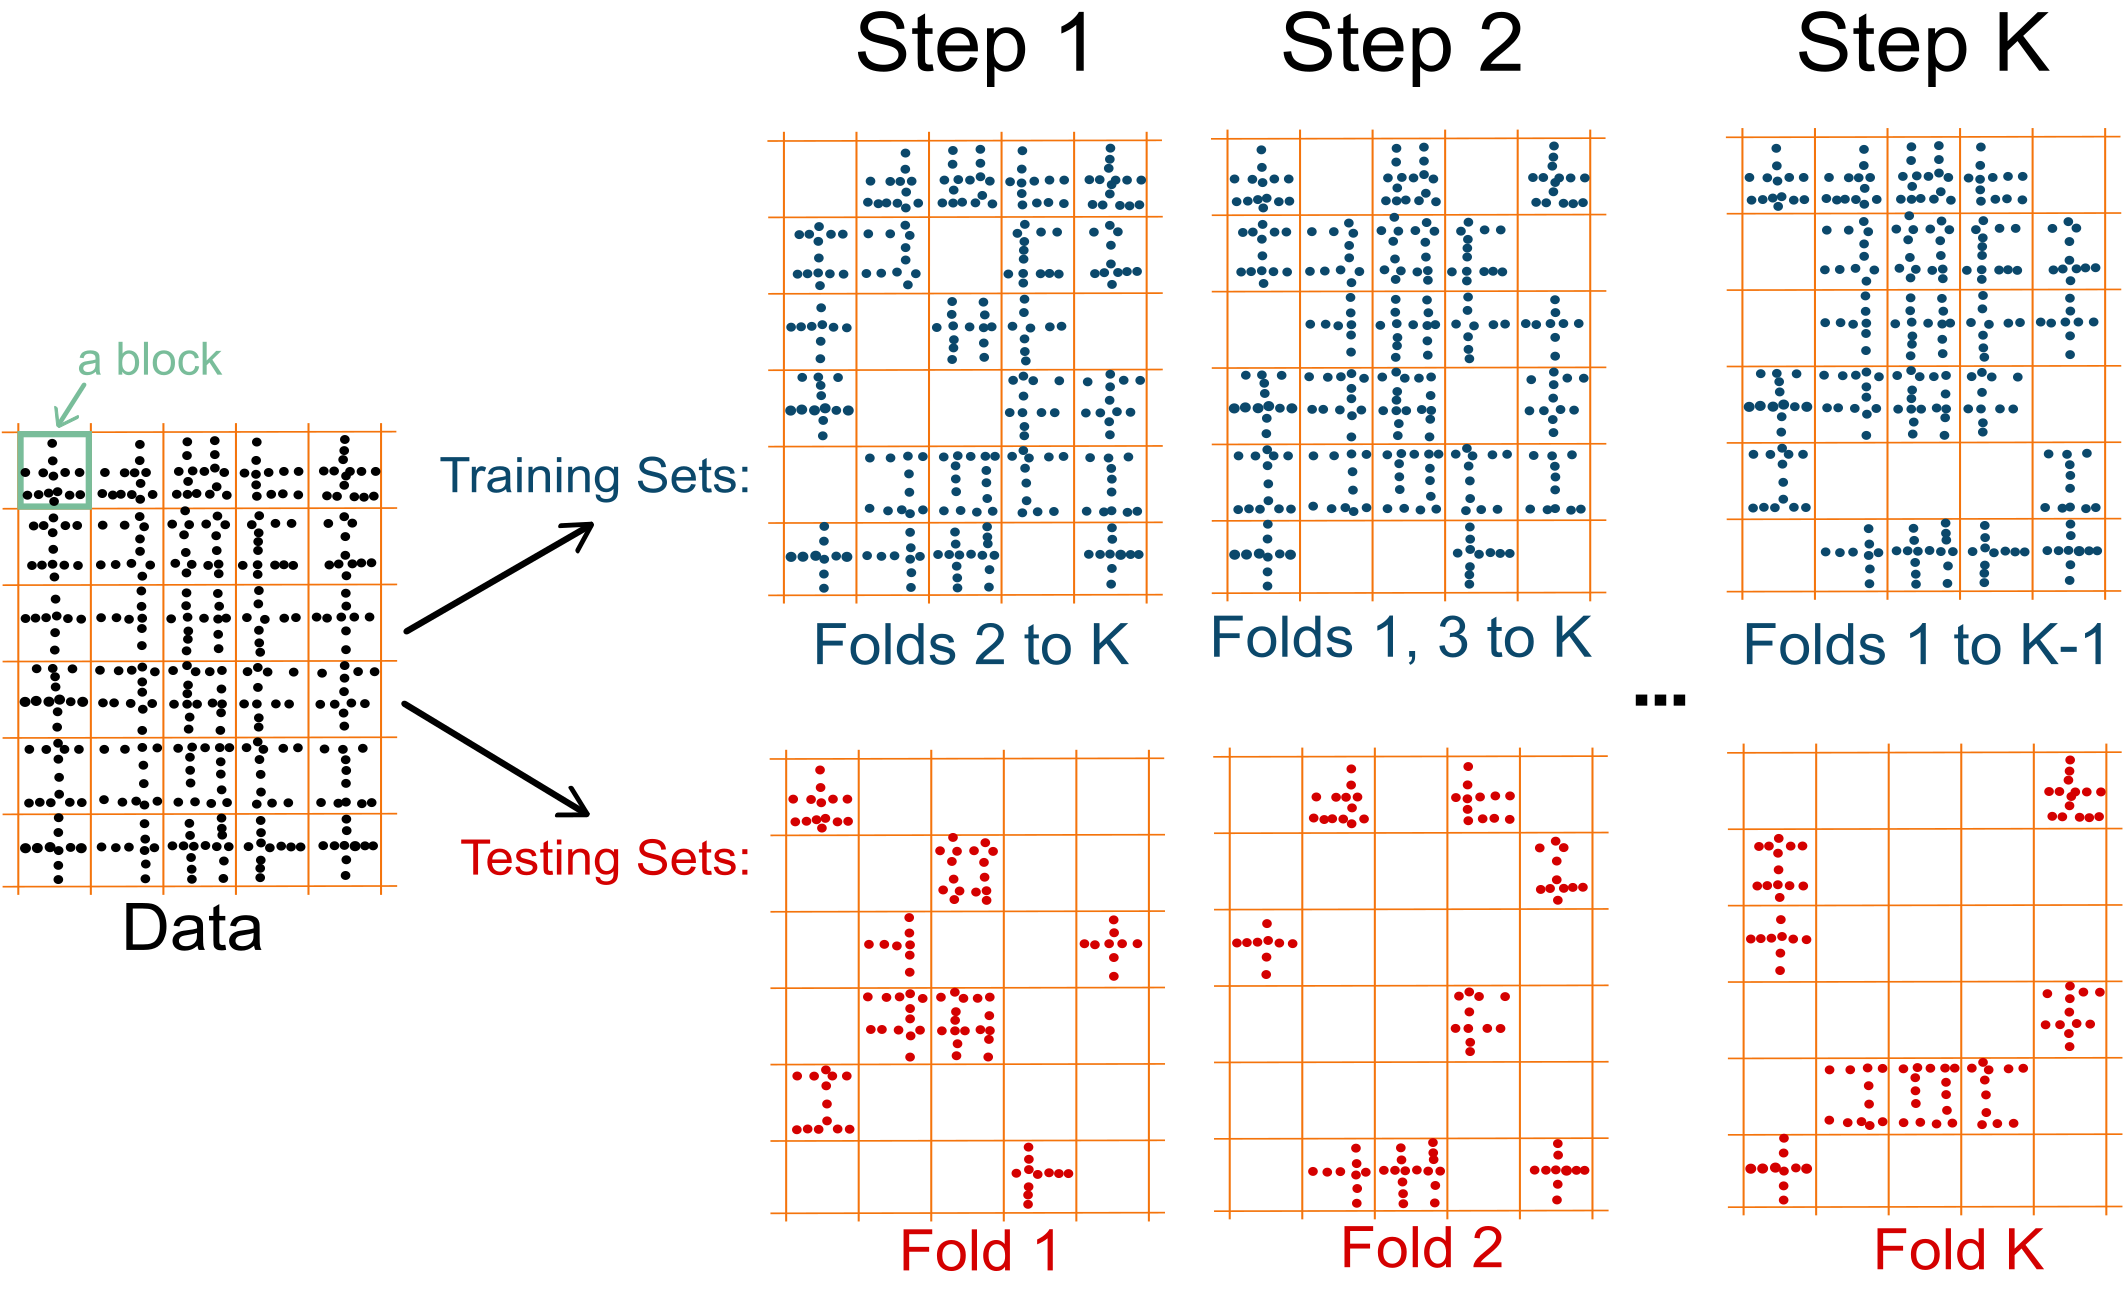
\includegraphics[width=1\linewidth]{eqs-gb-norm-of-b/figures/bk_cv.png}
  \caption{
    The Block K-Fold Cross Validation method. The black dots are the data, the orange blocks are the non-overlapping spatial blocks of a specified size, the blue dots are the training sets for each iteration and the red dots are the testing sets for each fold.
    }
  \label{fig:BK-CV}
\end{figure}

The model accuracy can be assessed though the Root Mean Square Error (RMSE) calculated between the observed data from the testing set (\textcolor{orange}{$\mathbf{d^o_{test}}$}) and the predicted total-field anomaly also on the testing set coordinates (\textcolor{orange}{$\mathbf{d_{test}}$}):

\begin{equation}
    \label{eq:rmse}
    \text{RMSE}_k = \sqrt{\dfrac{\sum\limits_{i=1}^L \left(\textcolor{orange}{{d^o_{test_i}}} - \textcolor{orange}{{d_{test_i}}}\right)^2}{L}}
    \ ,
\end{equation}

\noindent
for $L$ number of testing points. This BK-CV process is iterated until all the folds have been used for both testing and training (see Figure~\ref{fig:BK-CV}). The overall BK-CV RMSE is determined by taking the average of all the $\text{RMSE}_k$ values across the folds. This BK-CV is summarised in Algorithm~\ref{alg:BK-CV}.

\begin{algorithm}[!h]
    \setstretch{1.5}
    Split the data into blocks of a given size
    \;
    Split the blocks randomly into K folds, with roughly the same number of data per fold
    \;
    \For{each fold $k$}{
        Assign fold $k$ to the testing set and the remaining folds to the training set
        \;
        Estimate the parameters \textcolor{teal}{$\bar{\mathbf{c}}_k$} using the data from the training set and Equation~\ref{eq:normal_equations} or the gradient-boosted equivalent sources method
        \;
        Predict the total-field anomaly \textcolor{orange}{$\Delta T (x, y, z)$} on the coordinates of the testing set using Equation~\ref{eq:tfa_eqs}
        \;
        Calculate the $\text{RMSE}_k$ between the observed data from the testing set (\textcolor{orange}{$\mathbf{d^{o}_{test}}$}) and the predicted total-field anomaly (\textcolor{orange}{$\mathbf{d_{test}}$}) using Equation~\ref{eq:rmse}
        \;
    }
    Calculate the BK-CV RMSE by taking the average of all the $\text{RMSE}_k$ calculated for each fold.
    \BlankLine
    \setstretch{1}
    \caption{The Block K-fold Cross-Validation method.}
    \label{alg:BK-CV}
\end{algorithm}

To determine the optimal hyper-parameters for each layer, a range of values for damping and relative depth is systematically generated. \citet{dampney1969} suggests bounds of 2.5 to 6 times the average distance to the nearest neighbouring data points for the relative depth of equivalent sources. This range is utilised for the deep equivalent sources to ensure the regional long-wavelength signals are captured. For the shallow layer, a range of relative depths between the data heights and the deep layer are employed. Additionally, a range of $1 \times 10^{-10} \text{ to } 1 \times 10^{10}$ is used for the damping parameter $\mu$ (see Equation~\ref{eq:goal_function}). Once these ranges are defined, a comprehensive set of all the possible combinations of these hyper-parameters is created. For each combination, the BK-CV method (Algorithm~\ref{alg:BK-CV}) is employed to determine the corresponding BK-CV RMSE, which serves as the performance metric. The combination that yields the smallest BK-CV RMSE is then selected as the optimal set of parameters for the final equivalent source model.


%%%%%%%%%%%%%%%%%%%%%%%%%%%%%%%%%%%%%%%%%%%%%%%%%%%%%%%%%%%%%%%%%%%%%%%%%%%%%%%
\section{Synthetic data application}

To assess the accuracy of the interpolations, the method was applied to
synthetic datasets containing magnetic sources with varying shapes, sizes,
depths and induced magnetisations. To ensure consistency with real-world
conditions, the synthetic dataset was simulated using the flight lines from the
ICEGRAV 2013 aeromagnetic dataset \citep{ICEGRAV_data}, as detailed in
Section~\ref{sec:real_application}. These flight line coordinates were
projected using the Universal Polar Stereographic (UPS) projection,
specifically for the South Pole region. The Earth's main magnetic field
direction was set to match the IGRF orientation at the time of the original
measurements, with an inclination of -65$^\circ$ and declination of 35$^\circ$,
consistent with the real aeromagnetic dataset. A regional magnetic field was
modelled using the ``checkerboard'' function of Verde  \citep{verde2018} on a regularly spaced grid covering the entire survey area, located at 60 km beneath the surface with an oscillating height of 15 km amplitude. The magnetisation for the regional field was specified to have an inclination of -50$^\circ$, declination of 40$^\circ$ and magnitude of $5 \times 10^{12}$Am$^2$. A zero-mean pseudo-random Gaussian noise, with a standard deviation of 5 nT, was also applied to the regional field. Additionally, a deep dipole was added to study the effects of a truncated long-wavelength signal (see Section~\ref{sec:truncated_regional} for further details). This dipole was placed at coordinates (2250 km, 2730 km, -70 km), with a magnetisation of 55$^\circ$ inclination, 45$^\circ$ declination and $2 \times 10^{13}$Am$^2$ magnitude. The descriptions of the shallower synthetic sources can be found in Table~\ref{table:shallow_sources}, in which the characteristics of their shape, location and magnetisation are outlined.

\begin{table}[tb!]
\centering
\begin{tabular}{c c c c c c}
\toprule
 & Centre Location & \multicolumn{3}{c}{Magnetisation} \\
\cmidrule(lr){2-2} \cmidrule(lr){3-5}
Source & [x, y, depth] (km) & Inclination ($^\circ$) & Declination ($^\circ$) & Magnitude (Am$^2$) \\
\midrule
Oval & [1930, 3030, 6] & 75 & 60 & $2 \times 10^{10}$ \\
Irregular & [1960, 2980, 0.8] & -60 & 45 & $3 \times 10^{9}$ \\
Small Dipole & [1950, 2785, 0.5] & 45 & -65 & $5 \times 10^{10}$ \\
Small Dipole	& [2100, 3011, 0.5] & 45 & -65 & $5 \times 10^{10}$ \\
Small Dipole & [2110, 2955, 0.5] & 45 & -65 & $5 \times 10^{10}$ \\
Small Dipole & [2150, 2750, 0.5] & 45 & -65 & $5 \times 10^{10}$ \\
Linear (Dyke) & [2200, 2950, 1] & -70 & 80 & $1 \times 10^{9}$ \\
Linear (Dyke) & [2220, 2870, 5] & -70 & 80 & $2 \times 10^{9}$ \\
Irregular & [2230, 2820, 0.9] & 50 & 70 & $5 \times 10^{9}$ \\
Regional Dipole & [2260, 2830, 8] & -70 & 40 & $1 \times 10^{10}$ \\
\bottomrule
\end{tabular}
\caption{Descriptions of the shallower synthetic sources.}
\label{table:shallow_sources}
\end{table}

\subsection{Single and dual layer comparison}
\label{sec:single_vs_dual}

\begin{figure}[tb!]
\centering
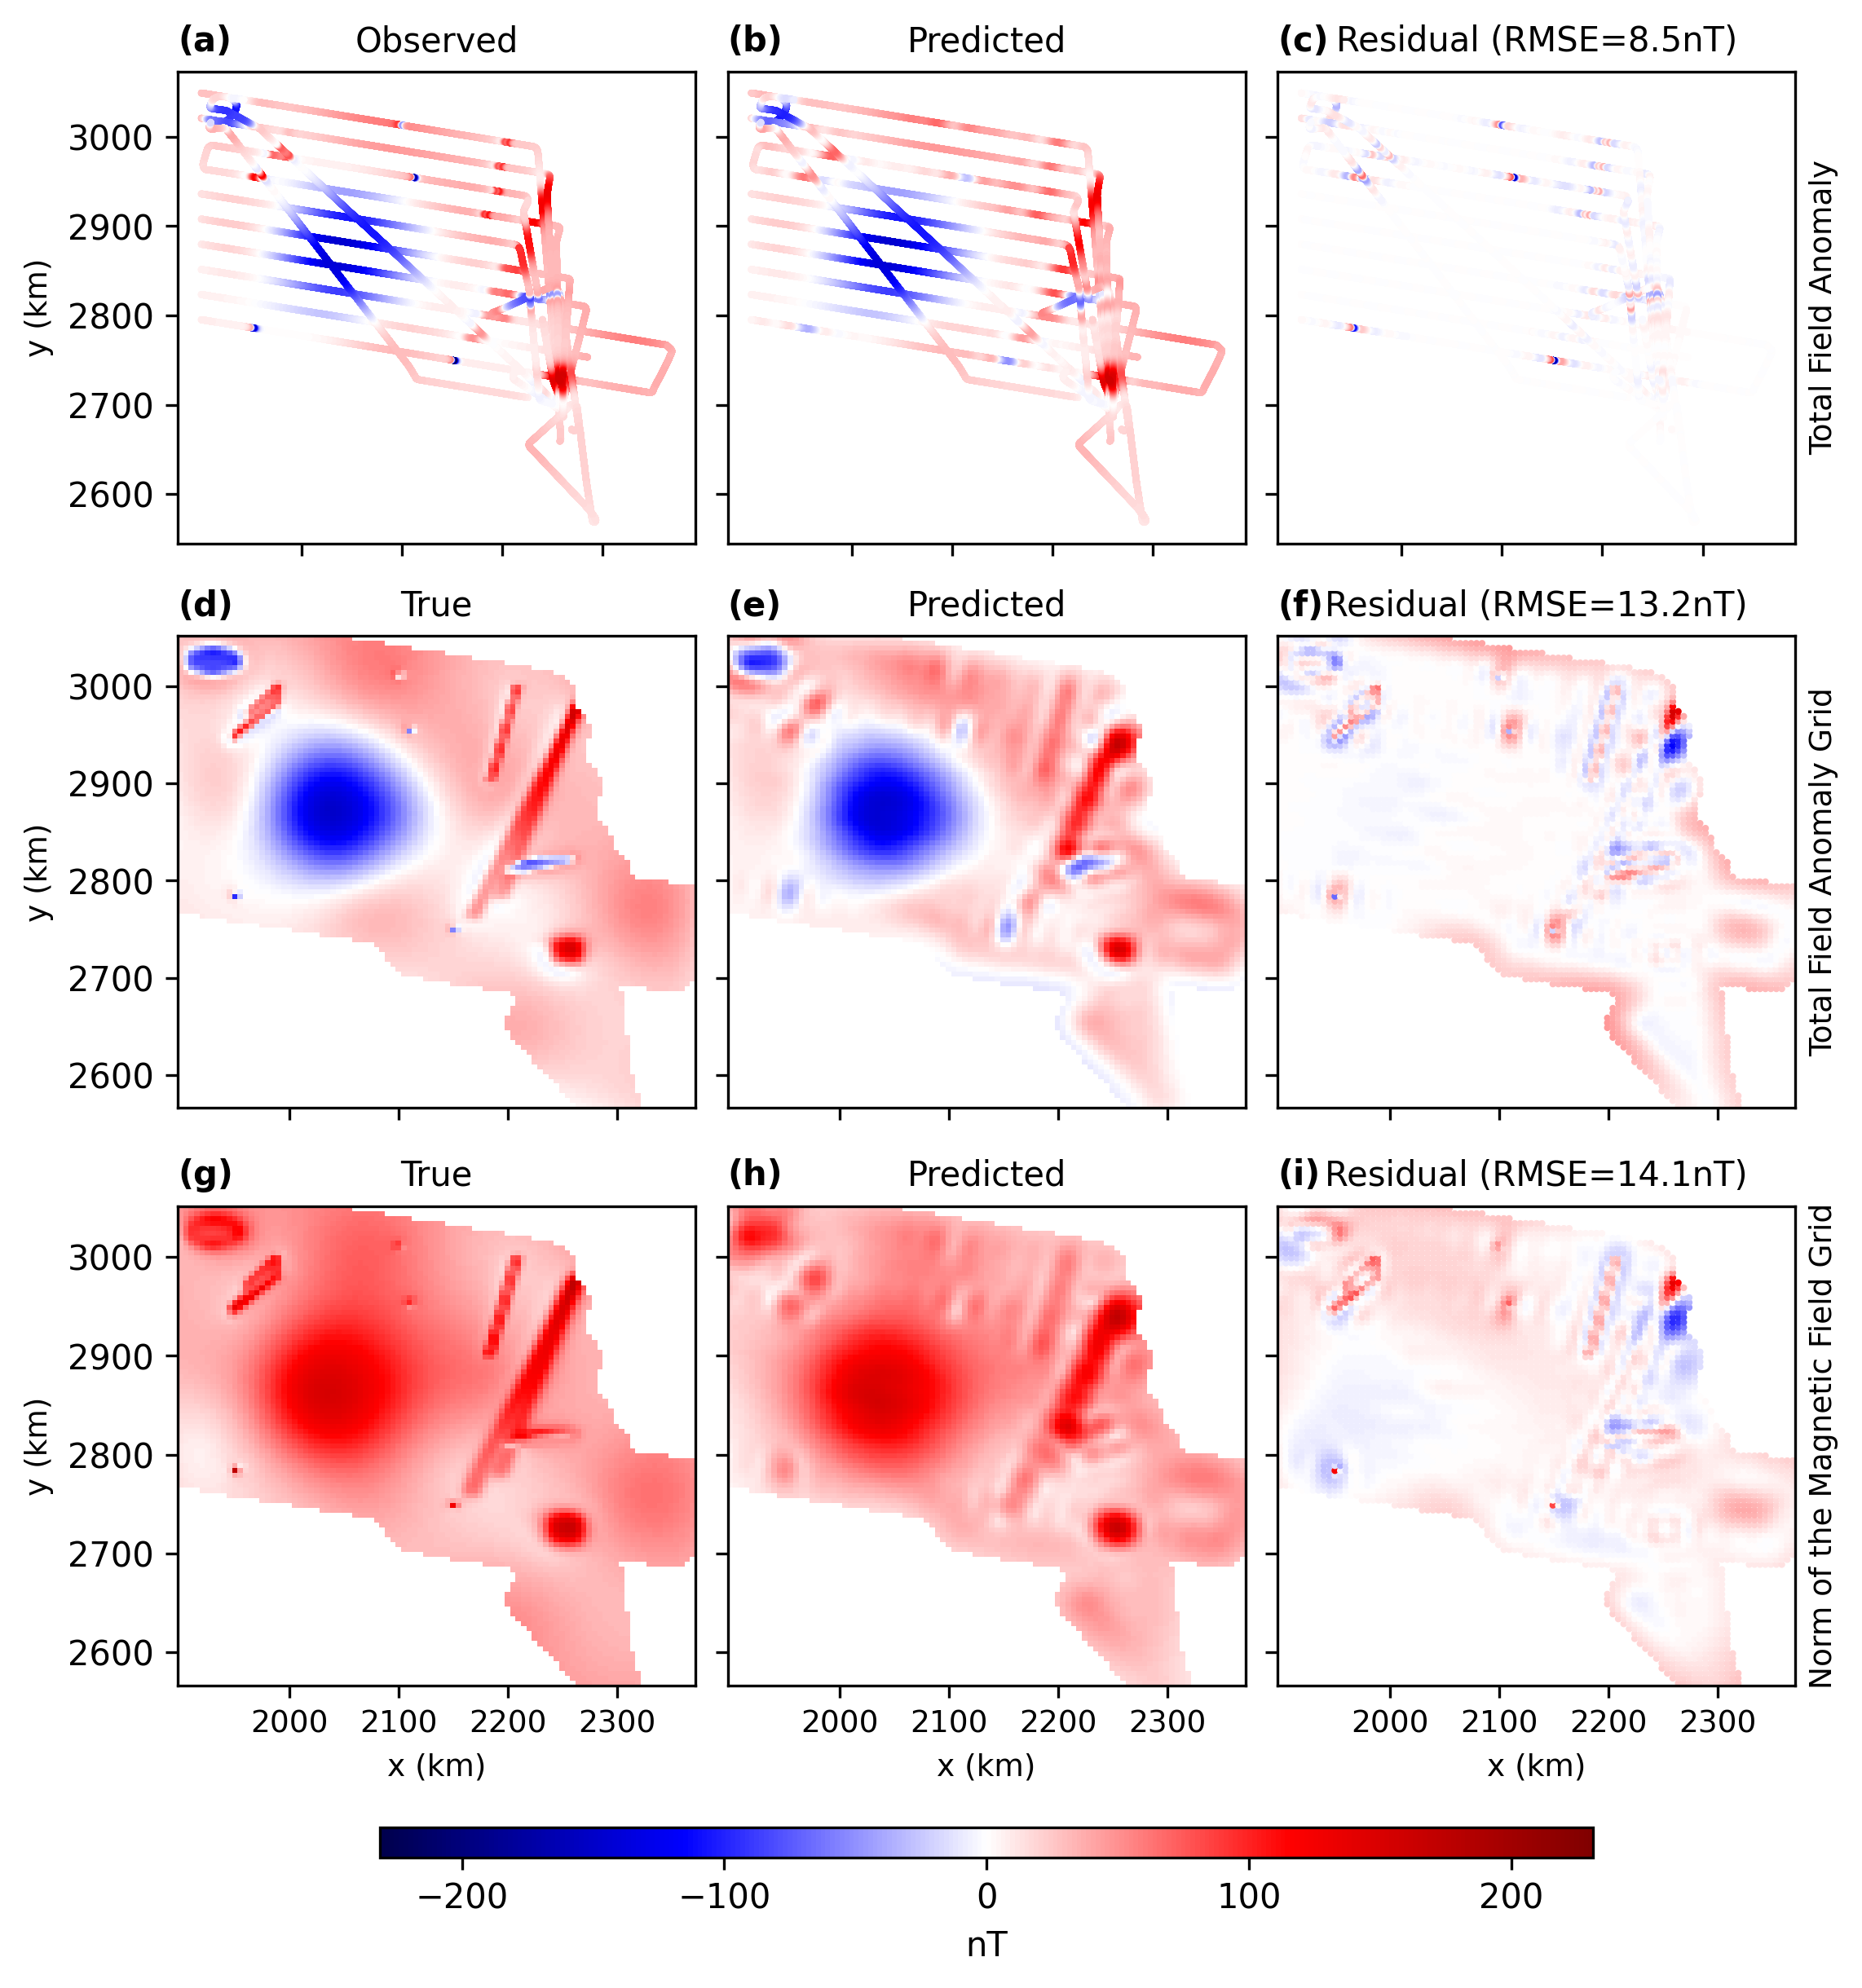
\includegraphics[width=1\linewidth]{eqs-gb-norm-of-b/figures/single_layer_synthetic.png}
\caption{
    Synthetic data and the predictions using a single layer of equivalent sources. a) observed total field anomaly of the synthetic data on the survey lines from the ICEGRAV survey \citep{ICEGRAV_data}, b) total field anomaly prediction on the survey lines, c) residual between the observed (a) and predicted (b) total field anomaly on the survey lines with a RMSE of 8.5 nT; d) true total field anomaly on a regular grid with 5 km spacing, e) predicted total field anomaly on regular grid with 5 km spacing, f) residual between the true (d) and predicted (e) total field anomaly on a regular grid with 5 km spacing and an RMSE of 13.2 nT; g) true norm of the anomalous magnetic field on a regular grid with 5 km spacing, h) predicted norm of the anomalous magnetic field on a regular grid with 5 km spacing, i) residual between the true (g) and predicted (h) norm of the anomalous magnetic field on a regular grid with 5 km spacing and an RMSE of 14.1 nT.
}
\label{fig:single_layer_synthetic}
\end{figure}

\begin{figure}[tb!]
\centering
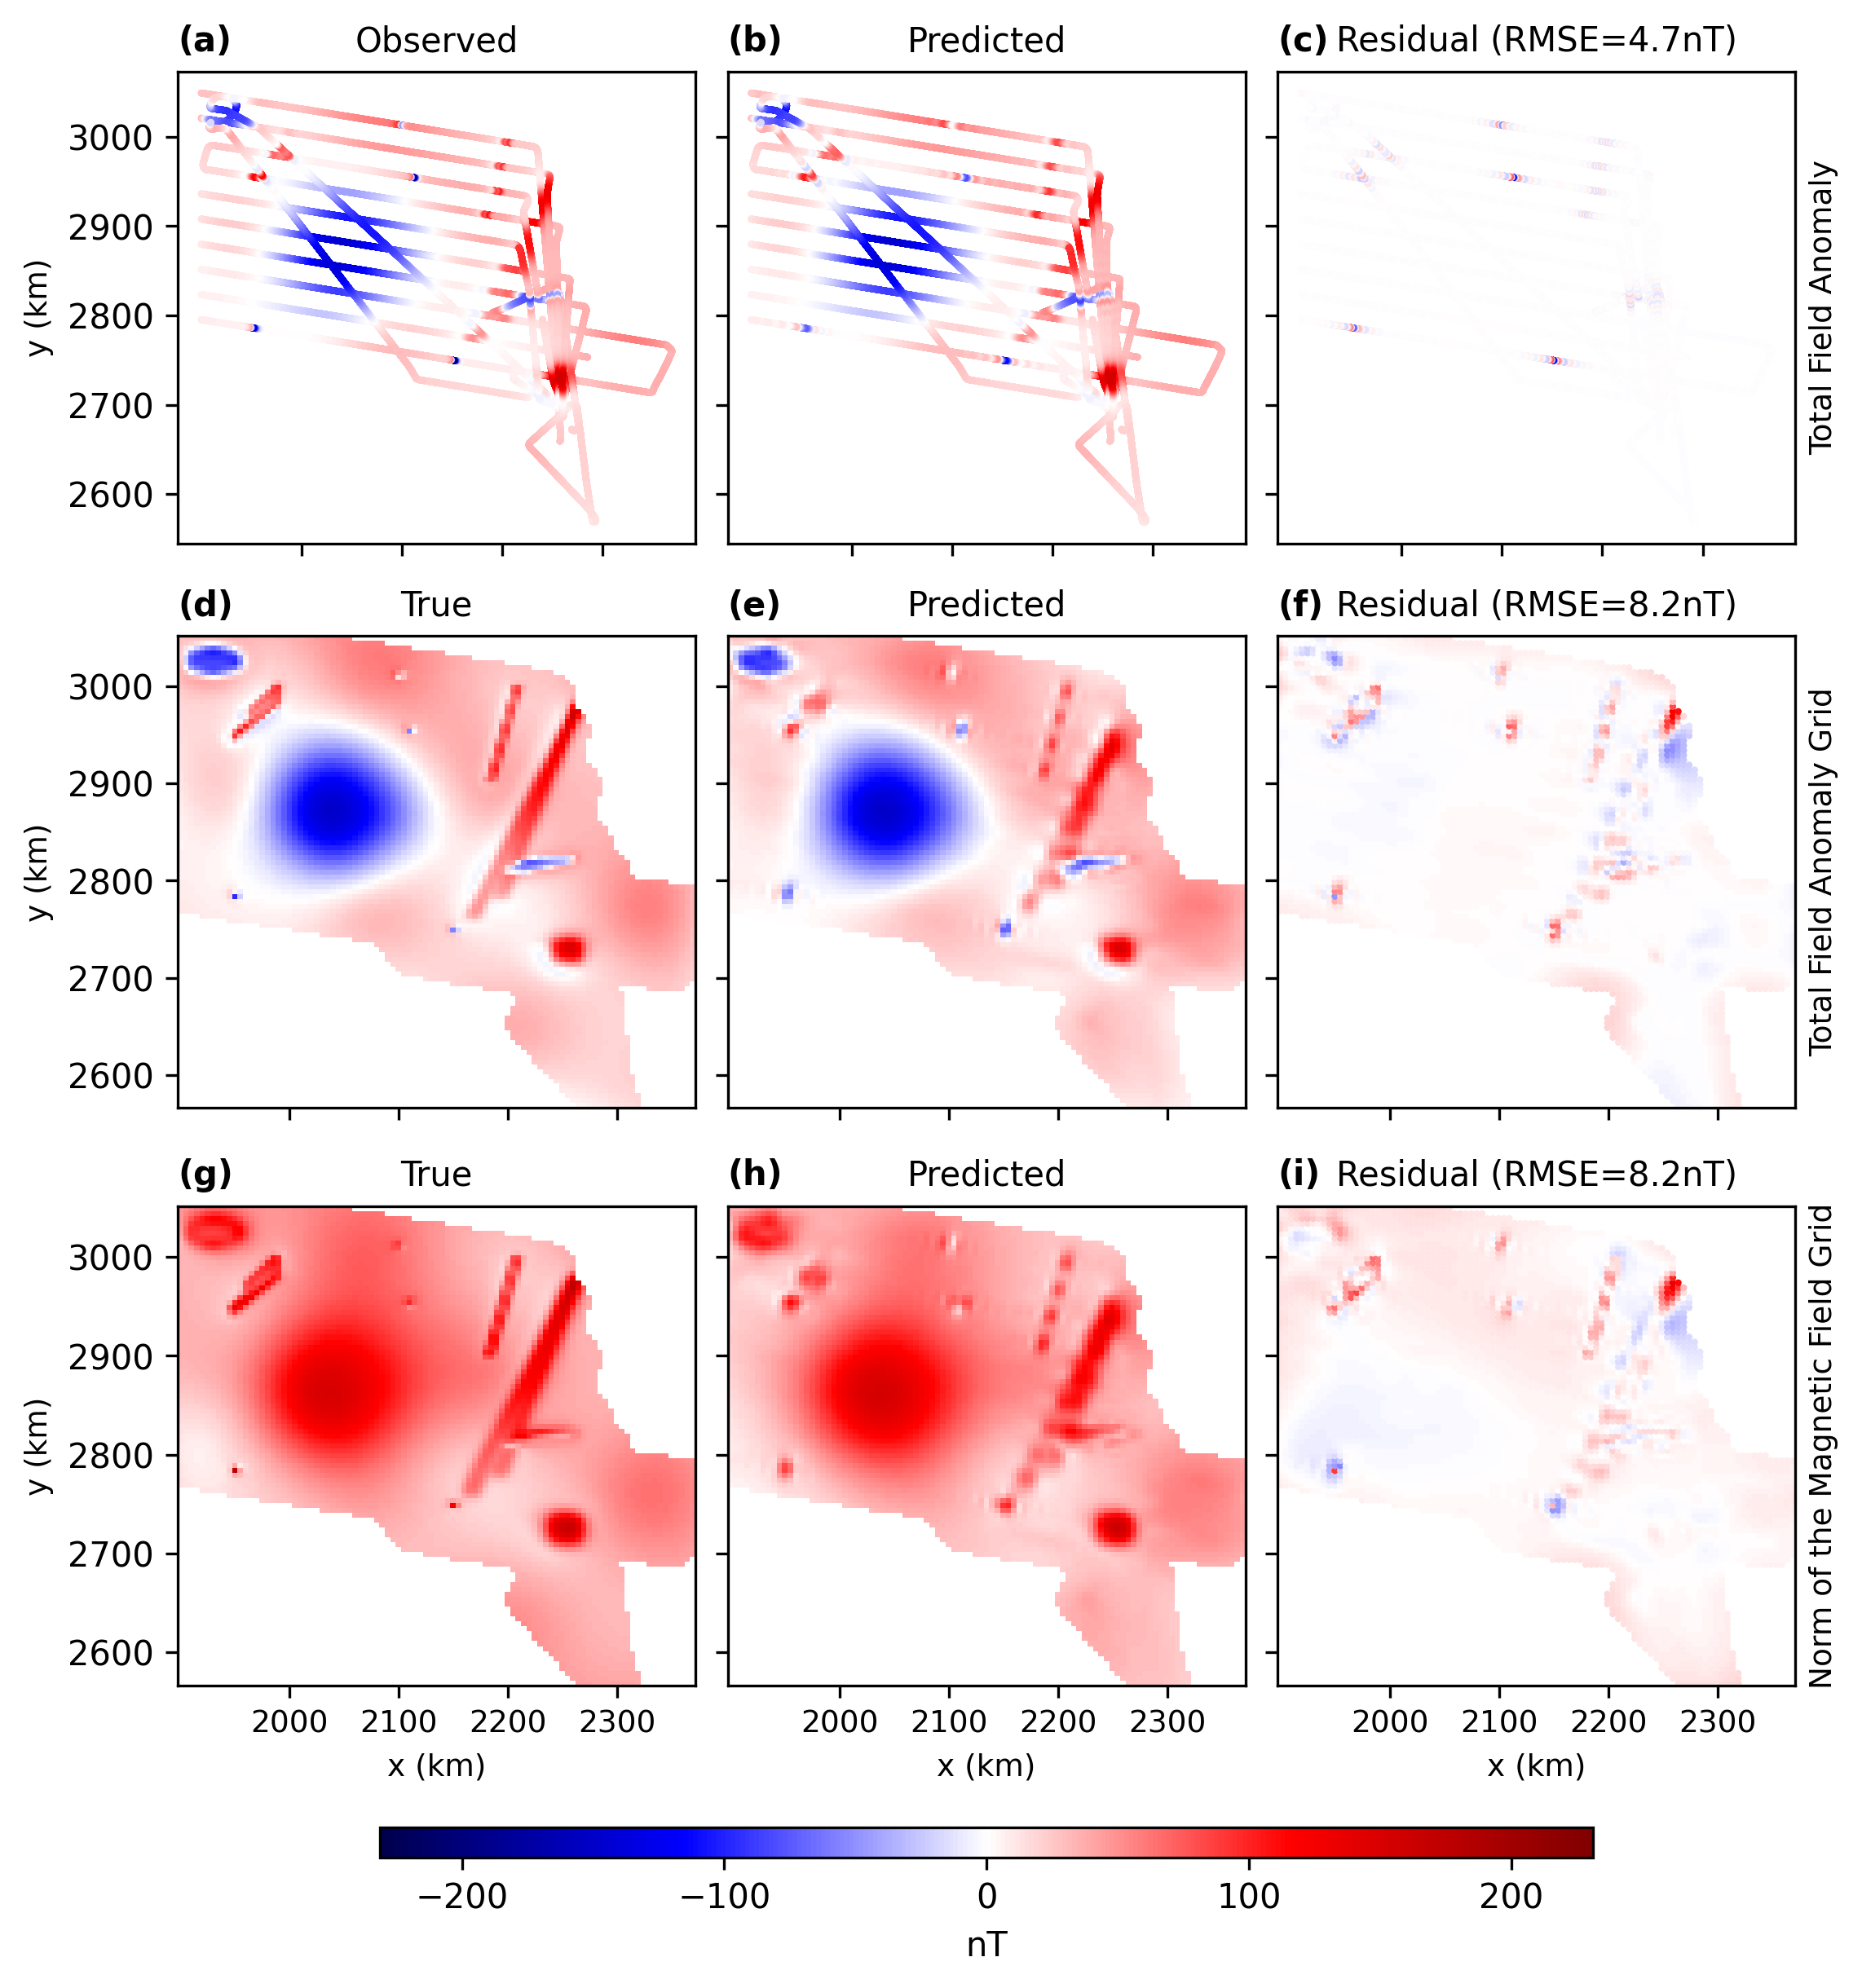
\includegraphics[width=1\linewidth]{eqs-gb-norm-of-b/figures/dual_layer_synthetic.png}
\caption{
    Synthetic data and the predictions using the dual layer equivalent sources. a) observed total field anomaly of the synthetic data on the survey lines from the ICEGRAV survey \citep{ICEGRAV_data}, b) total field anomaly prediction on the survey lines, c) residual between the observed (a) and predicted (b) total field anomaly on the survey lines with a RMSE of 4.7 nT; d) true total field anomaly on a regular grid with 5 km spacing, e) predicted total field anomaly on regular grid with 5 km spacing, f) residual between the true (d) and predicted (e) total field anomaly on a regular grid with 5 km spacing and an RMSE of 8.2 nT; g) true norm of the anomalous magnetic field on a regular grid with 5 km spacing, h) predicted norm of the anomalous magnetic field on a regular grid with 5 km spacing, i) residual between the true (g) and predicted (h) norm of the anomalous magnetic field on a regular grid with 5 km spacing and an RMSE of 8.2 nT.
}
\label{fig:dual_layer_synthetic}
\end{figure}

To assess the performance of a single versus a dual layer of equivalent sources, the single layer of equivalent sources was first applied using the gradient-boosted equivalent sources method (see Algorithm~\ref{alg:gradient_boosting}). To ensure optimal selection of the hyper-parameters, the block K-Fold cross-validation method (see Algorithm~\ref{alg:BK-CV}) was employed, using a block size of 30 km $\times$ 30 km over a wide range of parameter values. The optimal hyper-parameters, which resulted in the lowest cross-validated RMSE, were a damping value of $1 \times 10^{2}$ and a relative depth of 35 km. These optimised parameters were then used in the gradient-boosted equivalent sources with a window size of 250 km $\times$ 250 km. To further minimise the residuals of the inversion, the iteration over the windows was performed twice.

The resulting single-layer predictions for the total field anomaly along the survey lines, total field anomaly on a regular grid, and the norm of the anomalous magnetic field on a regular grid are presented in Figure~\ref{fig:single_layer_synthetic}. The prediction of the total field anomaly along the survey lines (Figure~\ref{fig:single_layer_synthetic}b) provides overall an accurate prediction, with an RMSE of 8.5 nT. However, it underestimates the magnitude of the four small, shallow dipoles, a pattern consistent with the predictions for both, the total field anomaly (Figure~\ref{fig:single_layer_synthetic}e) and the norm of the anomalous magnetic field (Figure~\ref{fig:single_layer_synthetic}h). Furthermore, the single layer model introduces undulating ripple effects at the edges of the sources, especially along the dykes. It also generates edges effects at the borders of the survey area (Figure~\ref{fig:single_layer_synthetic}e). These results highlight a key challenge when fitting both the short- and long-wavelength components simultaneously with a single layer.

To explore the potential benefits of a dual layer model, the dual layer equivalent source method (see Algorithm~\ref{alg:dual_layer}) was applied to the same synthetic dataset. The observed data was block averaged using different block spacings in order to determine the ideal size that is able to isolate the long-wavelength signals for the deep layer to fit. When the block spacing is too small, some of the short-wavelength signals are captured, resulting in the deep layer not capturing all of the regional long-wavelength signals due to trying to fit both long- and short-wavelengths. When the block spacing is too large, not all of the regional signals are captured either. The chosen ideal block spacing for this synthetic data was 25 km $\times$ 25 km.
To allow for more data points that fall along the survey boundary to be used, a padding of $0.2 \times $ the block spacing was added to the data border. The use of padding reduces the potential for edge effects at the borders that were seen in the single layer model. Using the block K-Fold cross-validation method (Algorithm~\ref{alg:BK-CV}) with a block size of 100 km $\times$ 100 km, the optimal hyper-parameters for the deep layer, which resulted in the lowest cross-validated RMSE, were a damping value of 1 and a relative depth of approximately 117 km ($6 \times$ the grid spacing). A larger block size was used for the deep layer because of the longer wavelength of the observed signals. The shallow layer was then fitted to the residuals from the deep layer in order to focus on fitting the shorter-wavelength signals, as well as correct potential errors caused by the deep layer. The gradient-boosted equivalent sources method (Algorithm~\ref{alg:gradient_boosting}) was utilised with a window size of 250 km $\times$ 250 km, matching the single layer model. To optimise the shallow layer’s hyper-parameters, the block K-Fold cross-validation method was applied with a block size of 30 km $\times$ 30 km (the same as the single layer model) to account for local variations in the data. The optimal hyper-parameters for the shallow layer, resulting in the lowest cross-validated RMSE, were a damping value of $1 \times 10^{2}$ and a relative depth of 17 km. The iteration over the windows of the gradient boosting method was repeated a second time to minimise potential errors in the initial windows selected in the iteration, similar to the single layer model.

The dual-layer results for the total field anomaly along the survey lines, total field anomaly on a regular grid, and the norm of the anomalous magnetic field on a regular grid are shown in Figure~\ref{fig:dual_layer_synthetic}. The dual layer model provides a significantly improved prediction of the total field anomaly along the survey lines (Figure~\ref{fig:dual_layer_synthetic} b), with an RMSE of 4.7 nT, particularly in capturing the four small dipoles. It also demonstrates the methods ability to interpolate onto regularly gridded lines and upward continue to a constant height (see Figure~\ref{fig:dual_layer_synthetic} e and h). Additionally, the regional field prediction is much smoother, with no edge effects at the survey borders or along the dykes, for both the total field anomaly and norm of the anomalous magnetic field. This will allow different surveys to be blended more easily. The dual layer model successfully reduces the undulating ripple effects near the edges of the sources. However, the dual-layer method does face challenges when predicting on the regular grid (Figure~\ref{fig:dual_layer_synthetic} e and h). Specifically, the method struggles with artifacts related to the flight lines, particularly along the dykes. The gaps between the survey lines appear more pronounced in these areas, leading to visible discontinuities. This issue could be addressed by adjusting the relative depth of the shallow layer, but in doing so may impact the accuracy of the small anomalies such as the small dipoles. Therefore, after using the Block K-Fold cross-validation to narrow the range of optimal values, visual inspection of the predictions is necessary in order to select the final value.

Overall, the dual-layer approach improves predictions, for both total field anomaly and norm of the anomalous magnetic field, by allowing the deep layer to capture the regional, long-wavelength signals, whilst the shallow layer focuses on the short-wavelength signals and corrects potential errors from the deep layer. This combination enhances the accuracy when compared to the single-layer approach, illustrating the advantages of using multiple layers of equivalent sources to model multi-scale sources. Applying padding to the deep layer reduces the edge effects along the survey borders, a common artefact when using a single layer model. The cross-validation method provides a more automated and efficient way to select optimal hyper-parameters. Additionally, the use of the gradient boosting method reduces the computational load and the processing time.

\subsection{Truncated long-wavelength anomaly}
\label{sec:truncated_regional}

\begin{figure}[tb!]
\centering
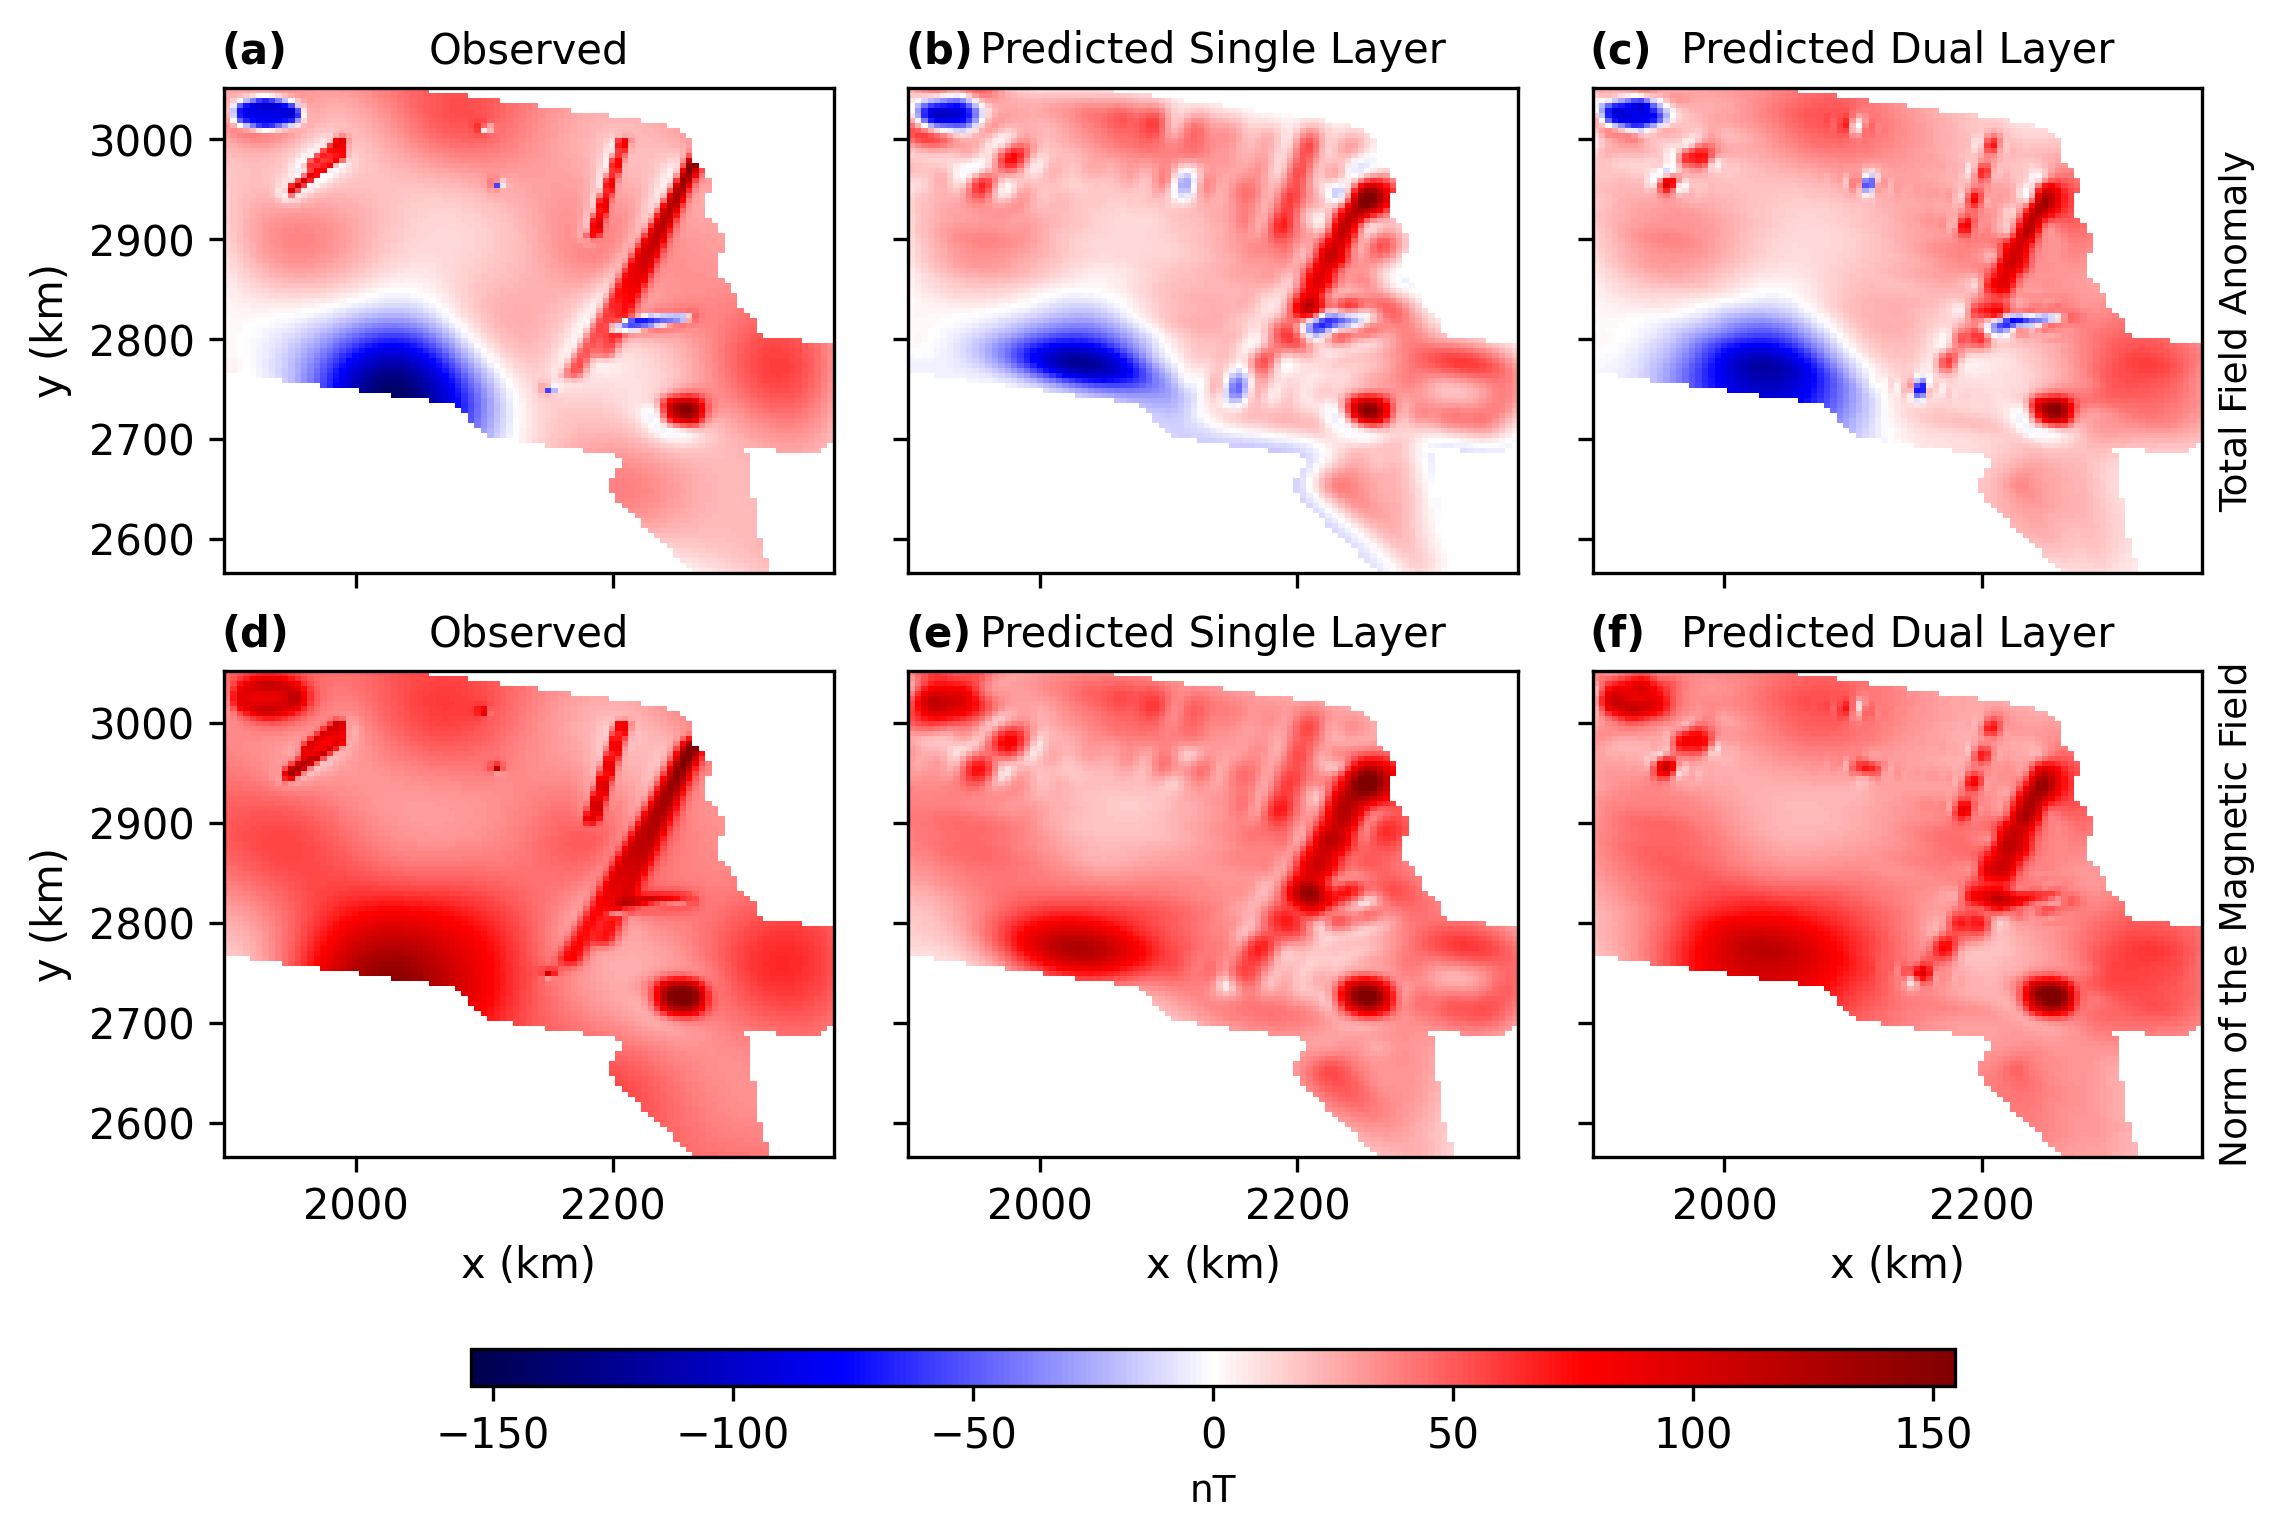
\includegraphics[width=1\linewidth]{eqs-gb-norm-of-b/figures/truncated_regional.png}
\caption{
    Synthetic data with a truncating regional dipole and the predictions using a single and dual layer of equivalent sources. a) true total field anomaly on a regular grid with 5km spacing, b) predicted total field anomaly on regular grid with 5km spacing using a single layer of equivalent sources, c) predicted total field anomaly on a regular grid with 5km spacing using the dual layer of equivalent sources; d) true norm of the anomalous magnetic field on a regular grid with 5km spacing, e) predicted norm of the anomalous magnetic field on a regular grid with 5km spacing using a single layer of equivalent sources, c) predicted norm of the anomalous magnetic field on a regular grid with 5km spacing using the dual layer of equivalent sources.
}
\label{fig:truncated_regional}
\end{figure}

\begin{figure}[tb!]
\centering
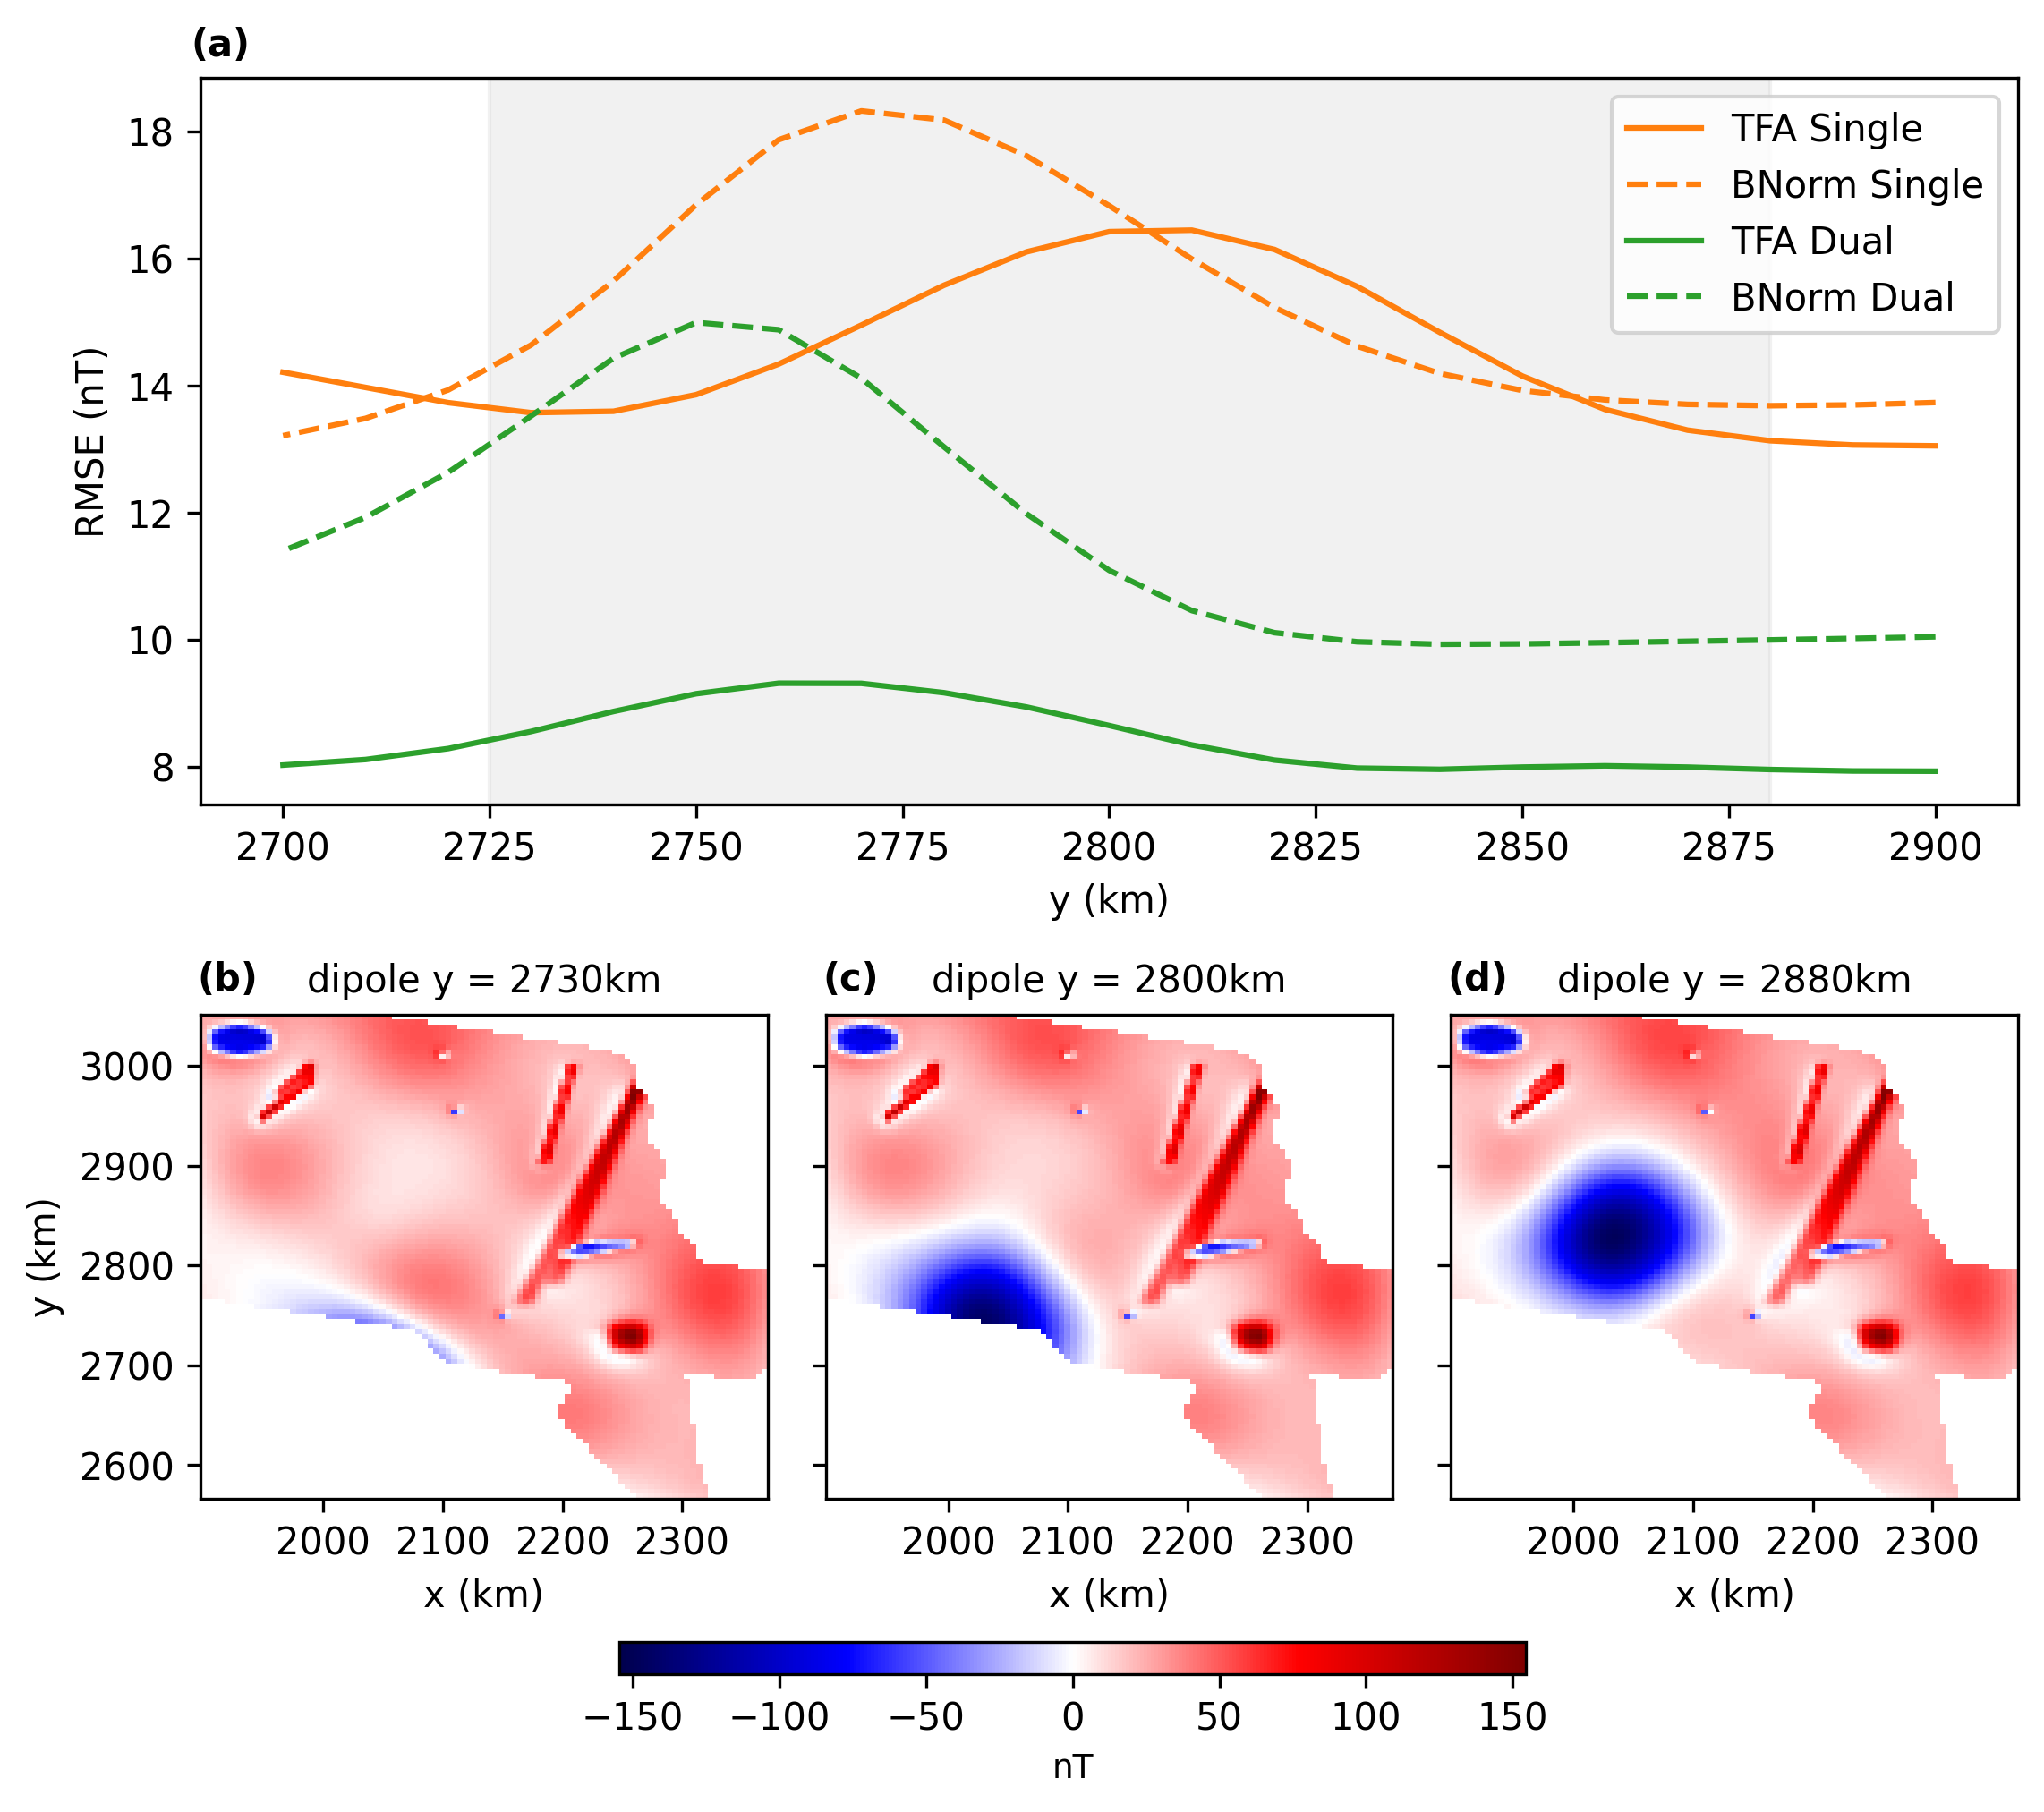
\includegraphics[width=1\linewidth]{eqs-gb-norm-of-b/figures/truncated_regional_rmses.png}
\caption{
    The Root Mean Square Error (RMSE) from the predictions of the total field anomaly (solid lines) and norm of the anomalous magnetic field (dashed lines) on a regular grid (with 5km spacing) as the regional dipole was shifted outside the survey boundary (a). The x-axis in (a) shows the y-coordinate at the top of the regional dipole. The RMSEs from the single-layer approach are shown in orange and the RMSEs from the dual-layer approach are shown in green. The shaded grey region in (a) highlights when the regional dipole was truncated and could partially be seen within the survey bounds. (b-d) shows the true total field anomaly on regular grids (with 5km spacing) with the regional dipole located at different y-coordinates as it was shifted outside the survey bounds. The y-coordinates at the top of the regional dipole are 2730km (b), 2800km (c) and 2880km (d).
}
\label{fig:truncated_regional_rmses}
\end{figure}

The impact of a truncated long-wavelength signal was also investigated further after observing the single-layer approach struggled to accurately predict the regional field. To assess this effect, both the single and dual layer models were applied while progressively moving a dipolar source with a long wavelength signal out of the survey boundary. An example of the truncated regional dipole is illustrated in Figure~\ref{fig:truncated_regional}). Both single and dual layer approaches appear to underestimate the magnitude of the truncated regional signal. Furthermore, the single-layer approach creates edge effects along the survey boundary resulting from the truncated regional signal (see Figure~\ref{fig:truncated_regional}b). On the contrary, the dual-layer approach mitigated these edge effects (see Figure~\ref{fig:truncated_regional}c), which was also noted in Section~\ref{sec:single_vs_dual}.

As the signal of the regional dipole became increasingly truncated, the RMSE for both models increased and then decreased back to the initial RMSE as the dipole influence became less visible (Figure~\ref{fig:truncated_regional_rmses}). The RMSE for the norm of the anomalous magnetic field (the grey shaded region of Figure~\ref{fig:truncated_regional_rmses}) significantly increased in comparison to the total field anomaly. The dual layer approach consistently exhibited a lower RMSE compared to the single-layer approach, suggesting it provides more reliable predictions overall in the presence of a truncated regional field signal. The impact of a truncated long-wavelength signal further highlights the importance of using a multi-layer approach when applying the equivalent sources technique.


%%%%%%%%%%%%%%%%%%%%%%%%%%%%%%%%%%%%%%%%%%%%%%%%%%%%%%%%%%%%%%%%%%%%%%%%%%%%%%%
\section{Real data application}
\label{sec:real_application}

\begin{figure}[tb!]
\centering
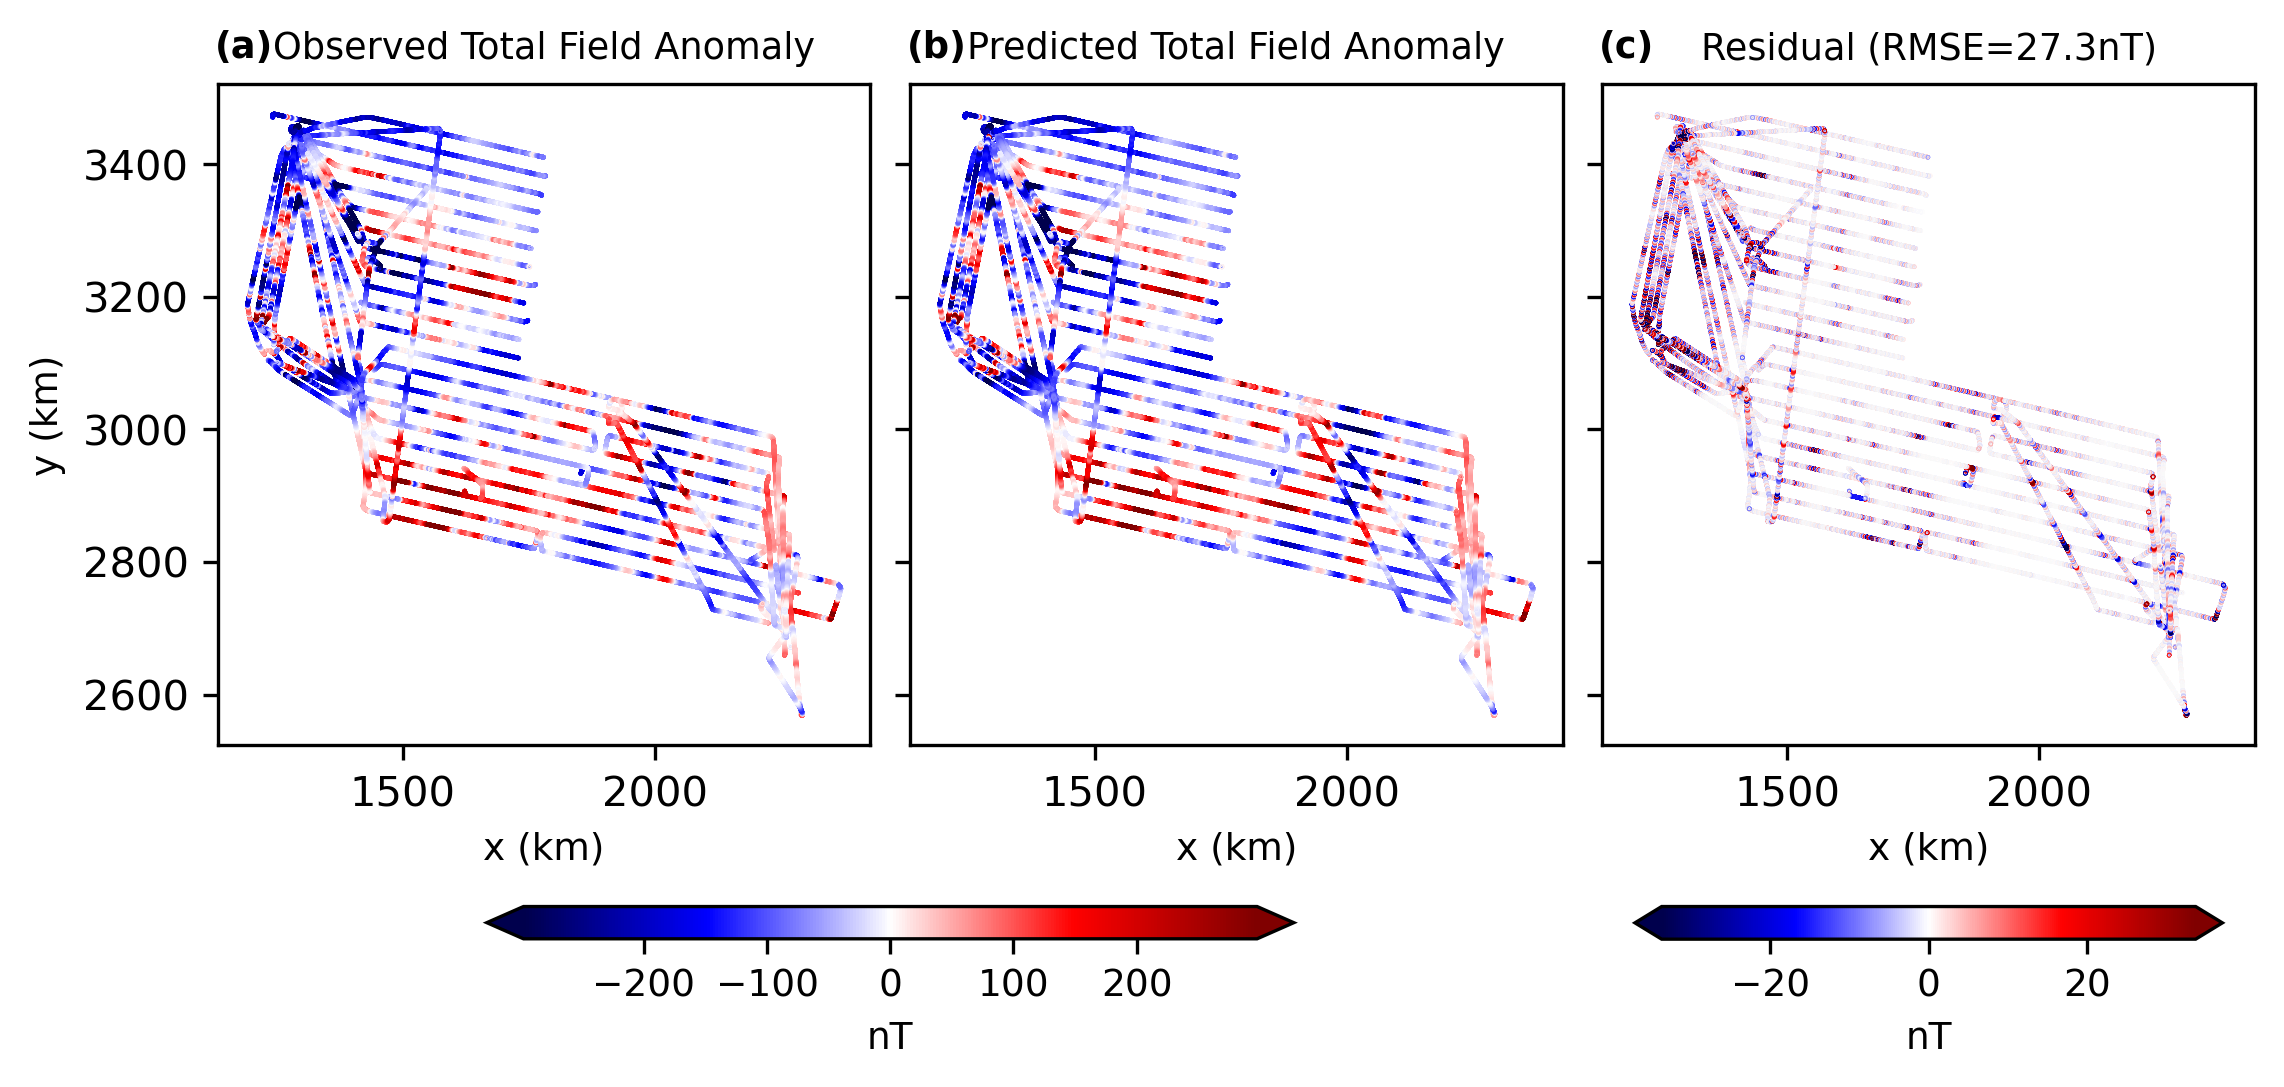
\includegraphics[width=1\linewidth]{eqs-gb-norm-of-b/figures/real_line_pred.png}
\caption{
    The real data and prediction on the flight lines using the dual-layer approach. The observed total field anomaly data of the ICEGRAV survey \citep{ICEGRAV_data} (a), the prediction (b) on the same survey lines using the dual layer of equivalent sources and the residual (c) between the observed and the predicted with an RMSE of 27.3 nT.
}
\label{fig:real_line_pred}
\end{figure}

The method was applied to the open-access aeromagnetic survey data from the ICEGRAV campaigns \citep{ICEGRAV_data}, which spanned from 2010 to 2013. The data covers parts of interior East Antarctica and the Antarctic Peninsula, including key areas such as the Dronning Maud Land ice stream systems and the Recovery Lakes drainage basin. This dataset was selected to showcase the effectiveness of the method on real-world data that features irregular survey flight lines, substantial spacing between those lines and varying line altitudes. The dataset’s distinctive characteristics, in terms of its vast geographical coverage, complex data collection and large amount of data points (404,363 observations), provide a robust and challenging test case for evaluating the method's performance in complex conditions.

\begin{figure}[tb!]
\centering
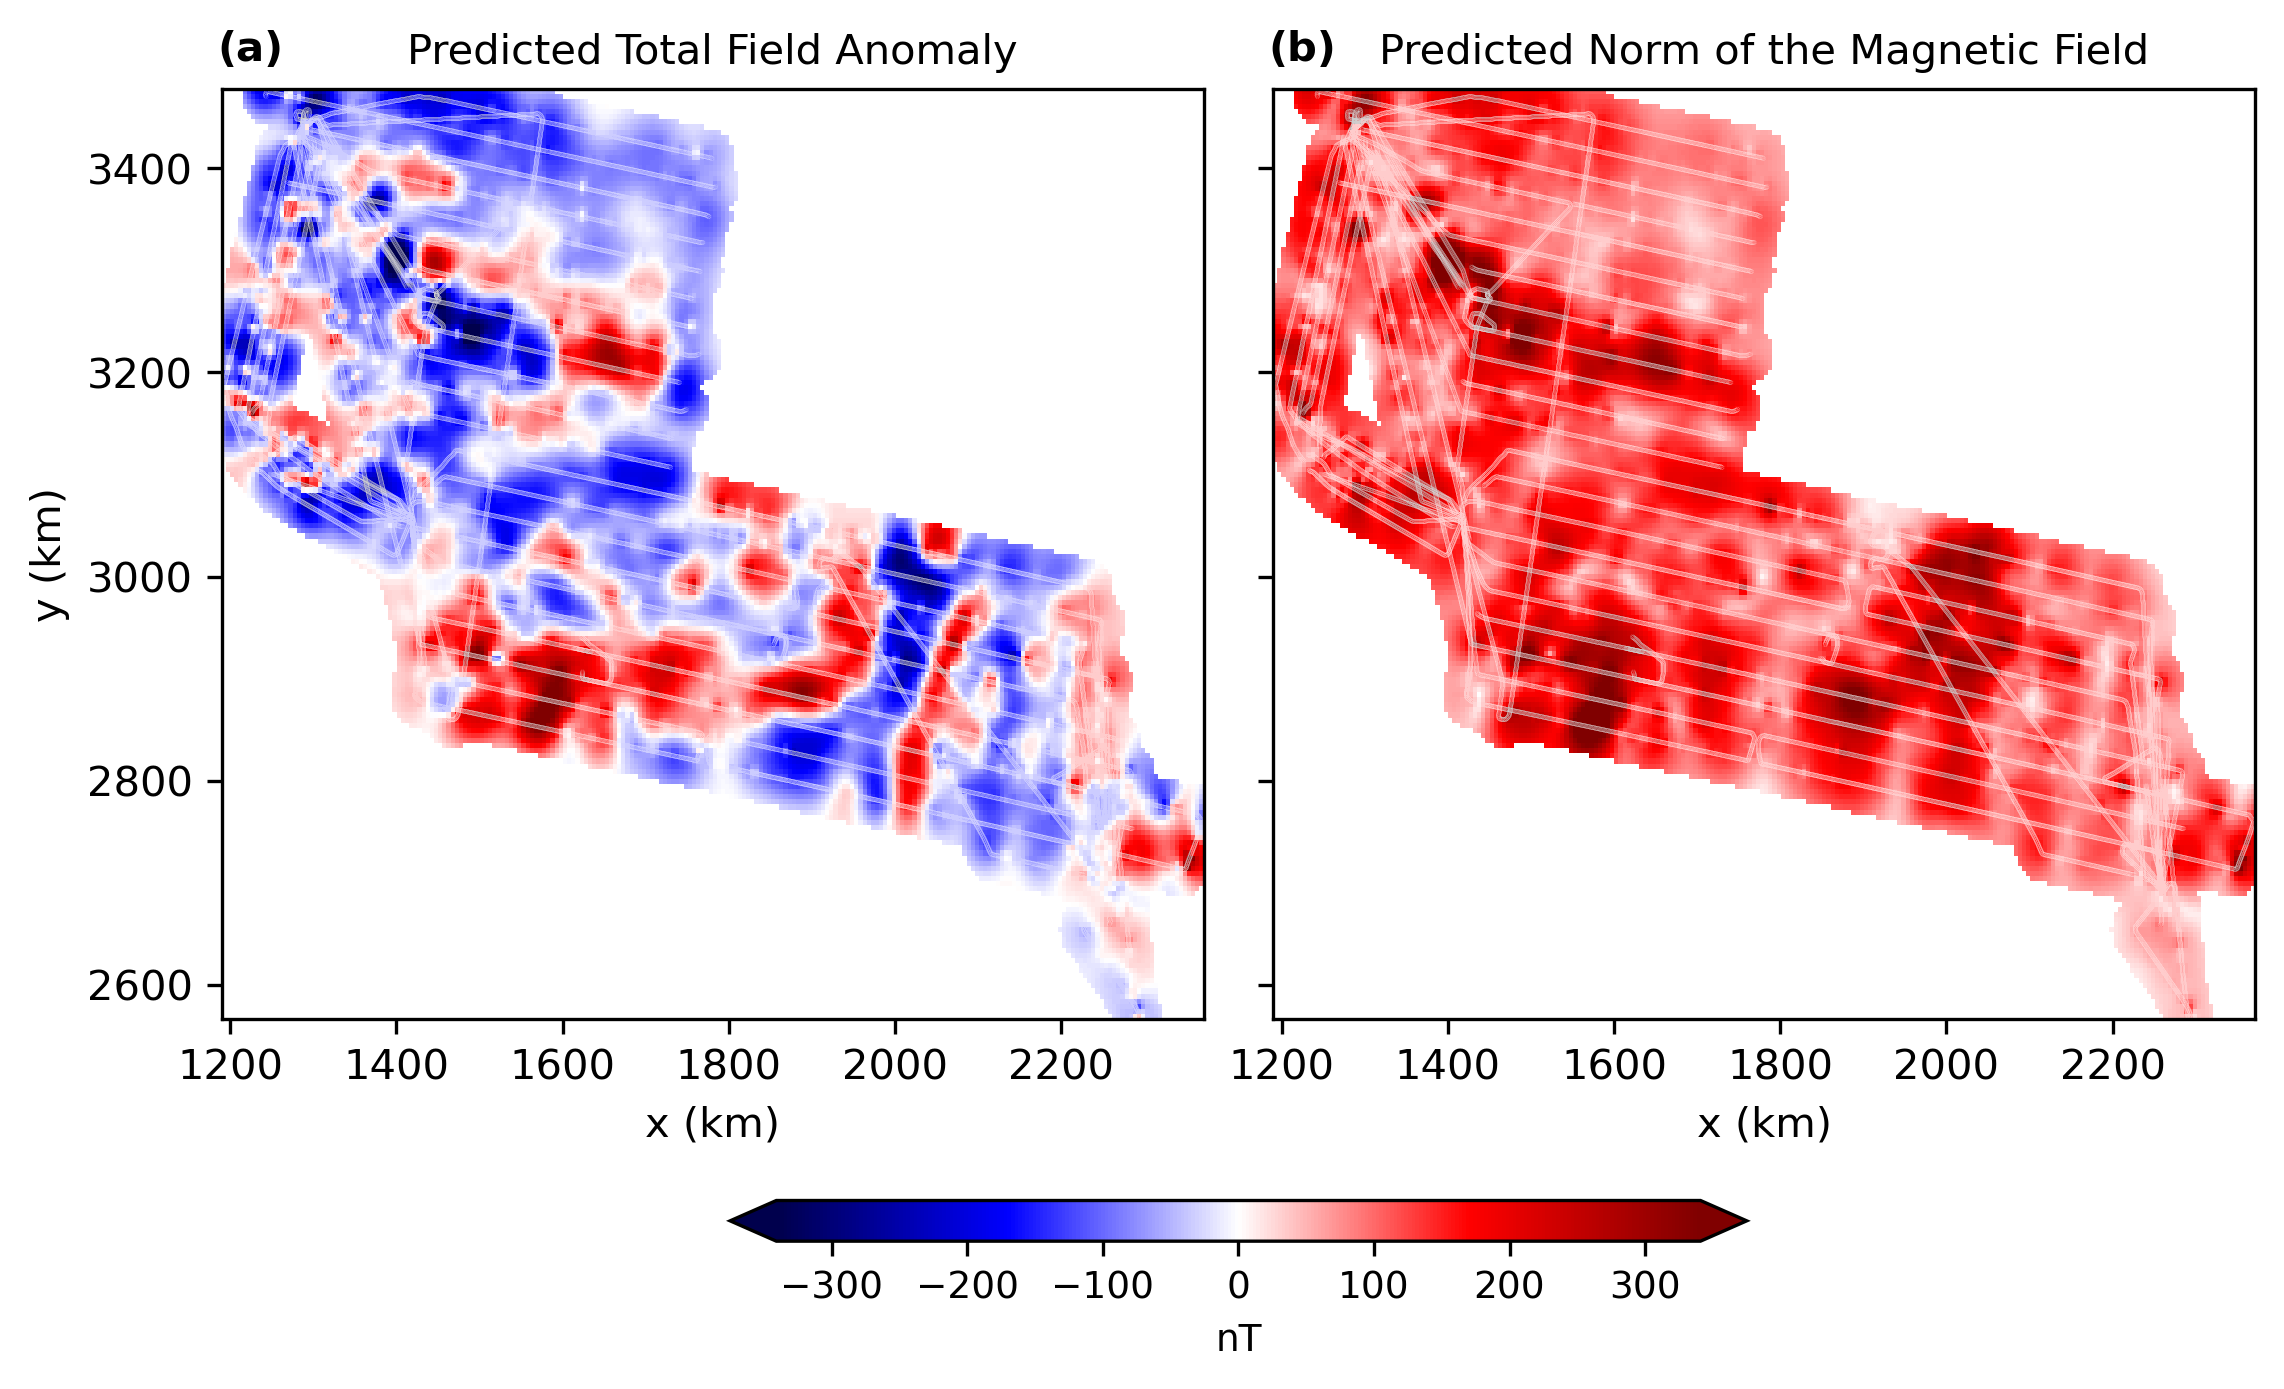
\includegraphics[width=1\linewidth]{eqs-gb-norm-of-b/figures/real_grid_pred.png}
\caption{
    The real data predictions on a regular grid using the dual-layer approach. The prediction of the total field anomaly (a) and norm of the anomalous magnetic field (b) of the ICEGRAV survey \citep{ICEGRAV_data} on a regular grid with 5km spacing. The survey lines are shown in white.
}
\label{fig:real_grid_pred}
\end{figure}

The coordinates of this dataset were first projected using the Universal Polar Stereographic (UPS) projection, specifically for the South Pole region. The dual layer equivalent source method (Algorithm~\ref{alg:dual_layer}) could then be applied to the observed data, which has already undergone some preprocessing \citep{ICEGRAV_data}. To fit the deep equivalent source layer, the observed data was block-averaged using different block spacings to determine the ideal size for isolating most of the long-wavelength signals. A block spacing of 15 km $\times$ 15 km, with a padding of $ 0.3 \times $ the block spacing, was selected by visual inspection. The padding allows for additional data points along the survey boundary, reducing the potential for edge effects at the borders. The block K-fold cross-validation method (see Algorithm~\ref{alg:BK-CV}) was applied with a block size of 200 km $\times$ 200 km to determine the optimal hyper-parameters which yield the lowest cross-validated RMSE. The chosen parameters were a damping value of 10 and a relative depth of approximately 55 km. The shallow layer was then fitted to the residuals from the deep layer using the gradient boosting method (see Algorithm~\ref{alg:gradient_boosting}) with a window size of 400 km $\times$ 400 km. The cross-validation method was utilised again to determine the optimal hyper-parameters for the shallow layer. Using a block size of 20 km $\times$ 20 km, the chosen parameters with the lowest cross-validated RMSE were a damping value of 100 and a relative depth of approximately 10 km. The gradient-boosted equivalent sources method (see Algorithm~\ref{alg:gradient_boosting}) was applied twice to the shallow layer to minimise potential errors in the initially selected windows of the iterations. The results for the total field anomaly along the survey lines are shown in Figure~\ref{fig:real_line_pred}. The dual layer provides a good prediction of the complicated dataset, with an RMSE of 27.3 nT.

The predictions of the total field anomaly and norm of the anomalous magnetic field on a regular grid are shown in Figure~\ref{fig:real_grid_pred}. Using a machine with 128 Gigabytes of RAM and an Intel Core i9 9980XE 3GHz processor with 18 cores, the dual layer approach took approximately 1 minute and 42 seconds to fit the 404,363 observed total field anomaly data point and predict the norm of the anomalous field on a regular grid. Here, the method demonstrates its ability to interpolate onto regularly gridded lines, as well as upward continue to a constant height. The grid predictions reveal numerous points with magnitude close to 0 nT, a pattern that is also present in the observed data. However, it remains uncertain whether these near-zero values represent real values or if they are artifacts introduced during the data preprocessing. If the latter is the case, more careful preprocessing may be necessary before applying the equivalent source method.



%%%%%%%%%%%%%%%%%%%%%%%%%%%%%%%%%%%%%%%%%%%%%%%%%%%%%%%%%%%%%%%%%%%%%%%%%%%%%%%
\section{Conclusion}

Different adaptations of the equivalent sources technique have been developed to improve the computational efficiency and accuracy of the predictions. However, many of these approaches still face challenges, such as the need for regularly gridded data at constant height, reliance on a stabilising parameter or the presence of border effects in the predictions. The dual-layer gradient-boosted equivalent sources tackles these limitations by:

\begin{enumerate}
    \item Using the dual-layer approach to improve the accuracy of the predictions and reduce the border effect.
    \item Using a two step approach, block-averaging and the gradient-boosted equivalent sources method to reduce the computational load.
    \item Applying block K-Fold cross-validation to guide optimal hyper-parameter selection for the model.
\end{enumerate}

The synthetic data tests demonstrate the dual-layer approach enhances the prediction accuracy over a single-layer approach by allowing the deeper layer to capture the regional, long-wavelength signals, whilst the shallower layer focuses on the short-wavelength signals. This approach also significantly improves predictions in cases where long-wavelength signals are truncated. Block-averaging the observed data reduces the number of sources needed in the deep layer, enabling it to focus on fitting the regional signals and decreasing the computational load. Applying padding to the deeper layer increases the number of data points along the survey border, reducing the potential for edge effects, a common issue with the equivalent sources technique.
To further enhance the computation efficiency, the gradient-boosted equivalent sources technique was utilised for fitting the shallow layer. This approach solves several smaller damped least-squares problems rather than solving one large problem. Repeating the window iterations of the gradient-boosting algorithm twice helped to minimise the residuals.

Further exploration of the single-layer model reveals an inherent trade-off: when placing the equivalent source layer deeper, it captures the regional, long-wavelength signals more effectively but struggles with the short-wavelength signals. Conversely, placing the equivalent source layer shallower, improves the capture of the short-wavelength signals but compromises the ability to determine the regional, long-wavelength signals. This balancing act emphasises the limitations of using a single-layer approach in modelling multi-scale sources and underlines the need for using a multi-layer model. Applying the dual-layer gradient-boosted equivalent sources to the ICEGRAV data demonstrated the method’s ability to successfully interpolate and upward continue the data on to a regular grid at a constant height, as well as predict the norm of the anomalous magnetic field. However, any artefacts from the data preprocessing will still be present in the final predictions, emphasising the importance of careful preprocessing before applying any gridding method.

The use of block K-Fold cross-validation has proven beneficial in narrowing the optimal range for the model hyper-parameters. However, visual inspection of the predictions still remains necessary to refine the final selection. This is due to the equivalent sources technique sometimes imprinting survey line artifacts onto the regular grid prediction. Further investigation into the ideal block size for cross-validation would also be beneficial, as well as the exploration of other spatial cross-validation methods that exist in the literature.



%%%%%%%%%%%%%%%%%%%%%%%%%%%%%%%%%%%%%%%%%%%%%%%%%%%%%%%%%%%%%%%%%%%%%%%%%%%%%%%
\section*{Data availability statement}

The Python source code used to produce all of the results and figures presented here are available at \url{https://github.com/\GitHubRepository} and
\url{https://doi.org/\ArchiveDOI} under the CC-BY license and the MIT
open-source license. This study also made use of the following open-source
scientific software: Numpy \citep{numpy} for linear algebra, matplotlib
\citep{Hunter2007} and PyGMT \citep{pygmt} for generating figures and maps,
pyproj \citep{pyproj} for data projection, Pandas \citep{pandas} for
manipulating tabular data, xarray \citep{xarray} for working with gridded data,
Verde \citep{verde2018} for the moving windows and interpolation and Harmonica \citep{harmonica} for potential-field data processing and modelling. The aeromagnetic data are available from the British Antarctic Survey \citep{ICEGRAV_data} under the UK Open Government Licence V3.0.

%%%%%%%%%%%%%%%%%%%%%%%%%%%%%%%%%%%%%%%%%%%%%%%%%%%%%%%%%%%%%%%%%%%%%%%%%%%%%%%
\section*{Acknowledgements}

We are indebted to the developers and maintainers of the open-source software without which this work would not have been possible. LU and IU were supported in part by start-up grant PRPI 22.1.09345.01.2 from Universidade de São Paulo. IU was also supported in part by a grant from the Earth Science Research Group, University of Liverpool.

%%%%%%%%%%%%%%%%%%%%%%%%%%%%%%%%%%%%%%%%%%%%%%%%%%%%%%%%%%%%%%%%%%%%%%%%%%%%%%%
\section*{CRediT author Contributions}

\textbf{India Uppal:} Conceptualisation, Methodology, Software, Validation, Formal Analysis, Inversitgation, Resources, Data Curation, Writing - Original Draft, Writing - Review and Editing, Visualisation, Project administration.
\textbf{Leonardo Uieda:} Conceptualisation, Methodology, Software, Resources, Writing - Review and Editing, Supervision.
\textbf{Vanderlei Coelho Oliverira Jr.:} Conceptualisation, Methodology, Writing - Review and Editing, Supervision.
\textbf{Richard Holme:} Conceptualisation, Writing - Review and Editing, Supervision.

\endgroup

%==============================================================================
\chapter{Magnetic microscopy inversion}

\begingroup
%%%%%%%%%%%%%%%%%%%%%%%%%%%%%%%%%%%%%%%%%%%%%%%%%%%%%%%%%%%%%%%%%%%%%%%%%%%%%%%
% Define information that is used to build the different documents, like the
% title, authors, affiliations, etc.

\newcommand{\Title}{Full vector inversion of magnetic microscopy images using Euler deconvolution as prior information}
\newcommand{\TitleShort}{Magnetic microscopy inversion}

\newcommand{\Year}{2024}
\newcommand{\SubmittedOn}{2023/06/01}
\newcommand{\AcceptedOn}{2024/04/11}

\newcommand{\GitHubRepository}{compgeolab/micromag-euler-dipole}
\newcommand{\ArchiveRepository}{10.6084/m9.figshare.22672978}

\newcommand{\PreprintDOI}{10.31223/X5QD5Z}
\newcommand{\Journal}{Geochemistry, Geophysics, Geosystems}
\newcommand{\JournalDOI}{10.1029/2023GC011082}

\newcommand{\Keywords}{%
  magnetic microscopy, geophysics, python, inverse problems, image processing
}

% NOTE: Author information is stored in the separate .tex files because the
% format varies between regular latex and journal formats...


\begin{summarybox}
    \noindent
    This chapter was originally published as
    \textbf{``Souza-Junior, G. F., Uieda, L., Trindade, R. I. F., Carmo, J. and
        Fu, R. R. (\Year). \Title{}. \textit{\Journal{}}.
    doi:\href{https://doi.org/\JournalDOI}{\JournalDOI}.''} under the
    terms of the CC-BY license. It is reproduced here under these terms.
\end{summarybox}

\section*{Abstract}
Paleomagnetic data is collected from bulk samples, containing a mixture of
stable and unstable magnetic particles. Recently, magnetic microscopy
techniques have allowed the examination of individual magnetic grains. However,
accurately determining the magnetic moments of these grains is difficult and
time-consuming due to the inherent ambiguity of the data and the large number
of grains in each image. Here we introduce a fast and semi-automated algorithm
that estimates the position and magnetization of dipolar sources solely based
on the magnetic microscopy data. The algorithm follows a three-step process: 1)
employ image processing techniques to identify and isolate data windows for
each magnetic source; 2) use Euler Deconvolution to estimate the position of
each source; 3) solve a linear inverse problem to estimate the dipole moment of
each source. To validate the algorithm, we conducted synthetic data tests,
including varying particle concentrations and non-dipolarity. The tests show
that our method is able to accurately recover the position and dipole moment of
particles that are at least \qty{15}{\um} apart for a source-sensor separation
of \qty{5}{\um}. For grain concentrations of 6250 grains/mm³, our method is
able to detect over 60\% of the particles present in the data. We applied the
method to real data of a speleothem sample, where it accurately retrieved the
expected directions induced in the sample. The semi-automated nature of our
algorithm, combined with its low processing cost and ability to determine the
magnetic moments of numerous particles, represents a significant advancement in
facilitating paleomagnetic applications of magnetic microscopy.


% \section{Introduction}

Several branches of Earth Sciences have demonstrated the importance of spatial resolution on a microscopic scale. For example, geochemistry and
geochronology applications have benefited from point-wise analyses
and compositional maps, allowing significant advances in the understanding of
igneous, metamorphic and sedimentary processes \citep{Verberne2020, Barnes2019,
Davidson2007}. Classical paleomagnetic techniques, on the other hand, consist
of analyzing bulk samples, where the magnetic signal of a single specimen is
the result of the sum of moments of a large assembly of ferromagnetic grains
\citep{Dunlop1997}. Typically, a standard paleomagnetic sample of
approximately \qty{10}{\cm\cubed} would contain hundreds of thousands
to millions of magnetic particles with sizes varying from magnetically stable
single-domain (SD) and vortex state grains (also called pseudo-single domain,
PSD) with sizes below \qty{1}{\um} \citep{Berndt2016}, to large ($\gg \qty{1}{\um}$) grains with
multi-domain (MD) magnetic structures, which are less stable magnetic recorders \citep{Dunlop1997}.
These large MD grains usually conceal the signal of the SD
and PSD grains and techniques of step-wise thermal and magnetic treatments are
needed to unveil this more stable and reliable magnetic record
\citep{Tauxe2018}. Recently, magnetic microscopy techniques opened the
possibility of obtaining magnetic field maps at the micro-scale and recovering the
magnetization of each grain, therefore enabling the separate analysis of stable
and unstable magnetic particles \citep{DeGroot2018, Lima2014, Weiss2007,
DeGroot2014}.

In order to apply magnetic microscopy to paleomagnetic studies, it is necessary
to recover from the magnetic images a large number of individual magnetic
moments, corresponding to at least tens of thousands of stable fine-grained
grains ($< \qty{1}{\um}$), in order to provide statistical significance to the
remanence vector \citep{Berndt2016}. Nowadays, with the development of
magnetic microscopy techniques, this task is no longer limited by the
resolution of magnetic microscopes \citep[\textit{e.g.}, ][]{Fu2020, Weiss2007, DeGroot2018,
Glenn2017, Lima2014, Reis2016}, but essentially by the intrinsic problem presented by the
ambiguity in the inversion of potential field data \citep{Barbosa2011,
DeGroot2021, Oliveira2015Estimation}, and ultimately by the lack of a fast and
automated way to recover such a large number of individual magnetic moments
from a set of magnetic images \citep{CortesOrtuno2022, Lima2013, Lima2009}. A
solution to the non-uniqueness of magnetic moment inversion is to add
independent prior information, such as the position of the ferromagnetic
particles \citep{Fabian2019}. This can be obtained, for example, from X-ray
computed tomography \citep[microCT; ][]{Fabian2019, DeGroot2021, DeGroot2018}.
Nonetheless, the standard microCT techniques do not provide adequate resolution
to resolve the finer and more stable magnetic grains \citep{CortesOrtuno2022,
DeGroot2021}, whereas other more sophisticated techniques such as ptychographic
X-ray tomography \citep[\textit{e.g.}, ][]{Maldanis2020} are not readily available and
too time-consuming to be routinely used in paleomagnetic studies.

Another route to be explored in the inversion of magnetic microscopy images is
to obtain all the information, \textit{i.e.} the magnetic moment and the position of the
sources, from the magnetic data itself \citep[\textit{e.g.}, ][]{Fu2020}. For that, we can
explore the techniques developed in exploration geophysics, in spite of the
differences between aeromagnetic surveys and magnetic microscopy
\citep{Lima2013}. Magnetic microscopy images commonly show the combined signal
of multiple magnetic particles and can vary greatly in wavelength, strength,
and spatial separation, depending on the natural remanent magnetization (NRM) and location of each particle. We
usually assume that the signal measured by the magnetic microscope is the
vertical component of the magnetic induction vector ($b_z$), the measurements
are performed on a regular grid with evenly spaced grid points and at a
constant height, and the data are contaminated with pseudorandom Gaussian noise and
long-wavelength noise (akin to a regional signal in aeromagnetic data). Here,
we provide a methodological routine to retrieve the individual magnetic moment
of ferromagnetic grains in magnetic microscopy images following the approach
devised by \citet{Oliveira2015Estimation} for the interpretation of
aeromagnetic anomalies. The method we propose allows one to quickly and
semi-automatically estimate the individual magnetic moment vector of the stable
magnetic carriers, making use of only the magnetic images themselves and an
assumption of approximately dipolar sources. If used on a large scale, the
method provides the means to scan large areas of the rock sample, attaining
potentially the number of magnetic moments necessary for paleomagnetic studies.


%%%%%%%%%%%%%%%%%%%%%%%%%%%%%%%%%%%%%%%%%%%%%%%%%%%%%%%%%%%%%%%%%%%%%%%%%%%%%%%
\section{Methodology}

We will achieve the goal of estimating the dipole moment of several individual
grains per image in a semi-automatic fashion by dividing the task into three
parts that can be performed independently:

\begin{enumerate}
\item \textbf{Source detection and separation:} Identify and spatially isolate
  the magnetic field caused by each source. We will do this through a
  combination of classic potential field data processing (\textit{total
  gradient amplitude}) and image processing (histogram stretching and
  equalization) and segmentation methods.
\item \textbf{Position estimation}: Estimate the 3D position of a magnetic
  particle based on the magnetic field measurements and the assumption of a
  dipolar source. This can be achieved by applying the Euler deconvolution
  method to the data segment identified in step 1.
\item \textbf{Magnetic moment inversion:} Estimate the 3-component dipole
  moment vector by inverting the magnetic field data using the position
  obtained from Euler Deconvolution as a constraint and the assumption of a
  dipolar source. This leads to a linear inverse problem that is stable and
  computationally efficient, particularly since the inversion is performed
  separately for each data segment identified in step 1.
\end{enumerate}

In the sections below, we describe the methodology used in each step of our
proposed workflow.

\subsection{Automatic source detection and separation}

Our first task is to automatically identify the signal of individual particles
and spatially segregate the data into windows, each containing the signal of a
single particle. We implemented the following workflow to achieve this:

\begin{enumerate}
\item Calculate the \textit{total gradient amplitude} (TGA), also known as the 3D analytic signal \citep{Roest1992Magnetic}, of the observed vertical   component of the magnetic field. The TGA is entirely positive and tends to be more concentrated on top of the magnetic field sources than the observed magnetic field. The derivative calculation also acts as a high-pass filter, removing long-wavelength noise from the data.
\item Apply a contrast stretching method to re-scale the TGA to a new range defined by the lower and upper percentiles of the data in order to highlight the weaker signals, either coming from small or from deep-seated particles.
\item Use the Laplacian of Gaussian (LoG) method \citep{VanderWalt2014} on the re-scaled TGA data to estimate the position and size of data windows containing the signal of each particle.
\end{enumerate}

The total gradient amplitude (TGA) was devised as a filter that can be applied
to aeromagnetic data to reduce the signal's dependence on the direction of
magnetization of the source and that concentrates the signal above the sources
\citep{Roest1992Magnetic, Nabighian2005}. The TGA is defined as the norm of the
gradient vector of a scalar field $f(x, y, z)$

\begin{equation}
\|\vec{\mathbf{\nabla}}f(x, y, z)\|  =
\sqrt{(\partial_x f)^2 + (\partial_y f)^2 + (\partial_z f)^2}
\ ,
\end{equation}

\noindent
in which $\partial_x f$ is the partial derivative of $f$ with respect to $x$
and likewise for the $y$ and $z$ directions. The partial derivatives are best
approximated using a second-order accurate central finite-difference scheme

\begin{equation}
\partial_x f(x, y, z) \approx
\dfrac{f(x + \Delta x, y, z) - f(x - \Delta x, y, z)}{2 \Delta x}
\ ,
\end{equation}

\noindent
and likewise for the $y$ and $z$ directions, in which $\Delta x$ is the grid
spacing (assumed to be equal in the $x$ and $y$ directions). For the $z$
component, $\Delta z = \Delta x$ and $f(x, y, z + \Delta z)$ and
$f(x, y, z - \Delta z)$ are calculated by upward and downward continuation,
respectively, performed in the wavenumber domain. The 2D maps of the $x$, $y$,
and $z$ derivatives will also be used in the Euler Deconvolution step described
below, which is known to be highly sensitive to noise in the derivatives
\citep{Saleh2012}. This is why we prefer the finite-differences-based
derivatives, which are less prone to amplifying short-wavelength noise than
those calculated in the wavenumber domain through the Fast Fourier Transform
(FFT).

Once we have obtained a TGA image, we apply a contrast stretching method to
re-scale the TGA values in order to highlight the weaker signals present in the
image. This is a necessary step to make sure that the blob detection algorithm
is able to identify particles causing both weak and strong signals. The
following contrast stretching operation is performed per pixel of the TGA image

\begin{equation}
\text{TGA}_{rescaled} =
2\left(\dfrac{\text{TGA} - v_{min}}{v_{max} - v_{min}}\right) - 1
\ ,
\end{equation}

\noindent
in which $v_{min}$ and $v_{max}$ are the upper and lower bounds of TGA values
that will be stretched to the range $[0, 1]$. By experimentation, we found
that values of $v_{min} = 1^\text{st}$ and $v_{max} = 99^\text{th}$
percentiles of the TGA range work well on real magnetic microscopy datasets.

The re-scaled TGA image is then used as input for a Laplacian of Gaussian (LoG)
blob detection algorithm \citep{Kong2013}. This method is able to identify the
location and size of multiple windows in the image containing ``blobs''. In our
case, the blobs are the re-scaled TGA field of each particle and the LoG method
detects the local TGA maxima. The LoG method is particularly well suited for
the detection of bright blobs on a dark background at the expense of a longer
computation time \citep{Han2016}. For the image sizes routinely found in
magnetic microscopy, the computation is fast and only needs to be performed
once per image. To avoid issues of source truncation in the following steps, we
exclude windows that are on or close to the borders of the datasets.

\subsection{Euler Deconvolution}

Once the locations and sizes of the windows containing the isolated signals of
each particle are determined, we can apply the Euler Deconvolution (ED)
estimate of the $x$, $y$, and $z$ positions of the center of the particles
under a dipolar approximation. This technique was first proposed by
\citet{Thompson1982} under the name EULDPH and later extended to three
dimensions and renamed ``Euler Deconvolution'' by \citet{Reid1990}. ED is
traditionally performed on a set of moving windows that scan the entire
dataset, producing a large scatter of position estimates, most of which are
spurious \citep{Silva2003}. This is only done because it is impractical to
segment an aeromagnetic dataset into individual anomalies. Fortunately,
magnetic microscopy images often contain fewer elongated features (\textit{e.g.}, dikes and
suture zones) and regional signals (\textit{e.g.}, Curie depth variations) that are
difficult to separate. This makes it possible for us to produce isolated
signals for each magnetic particle through the source detection step described
above. Since each data window contains only the signal of a single particle, we
are able to apply ED and generate only a single position estimate per particle.

\begin{figure}[tb]
\centering
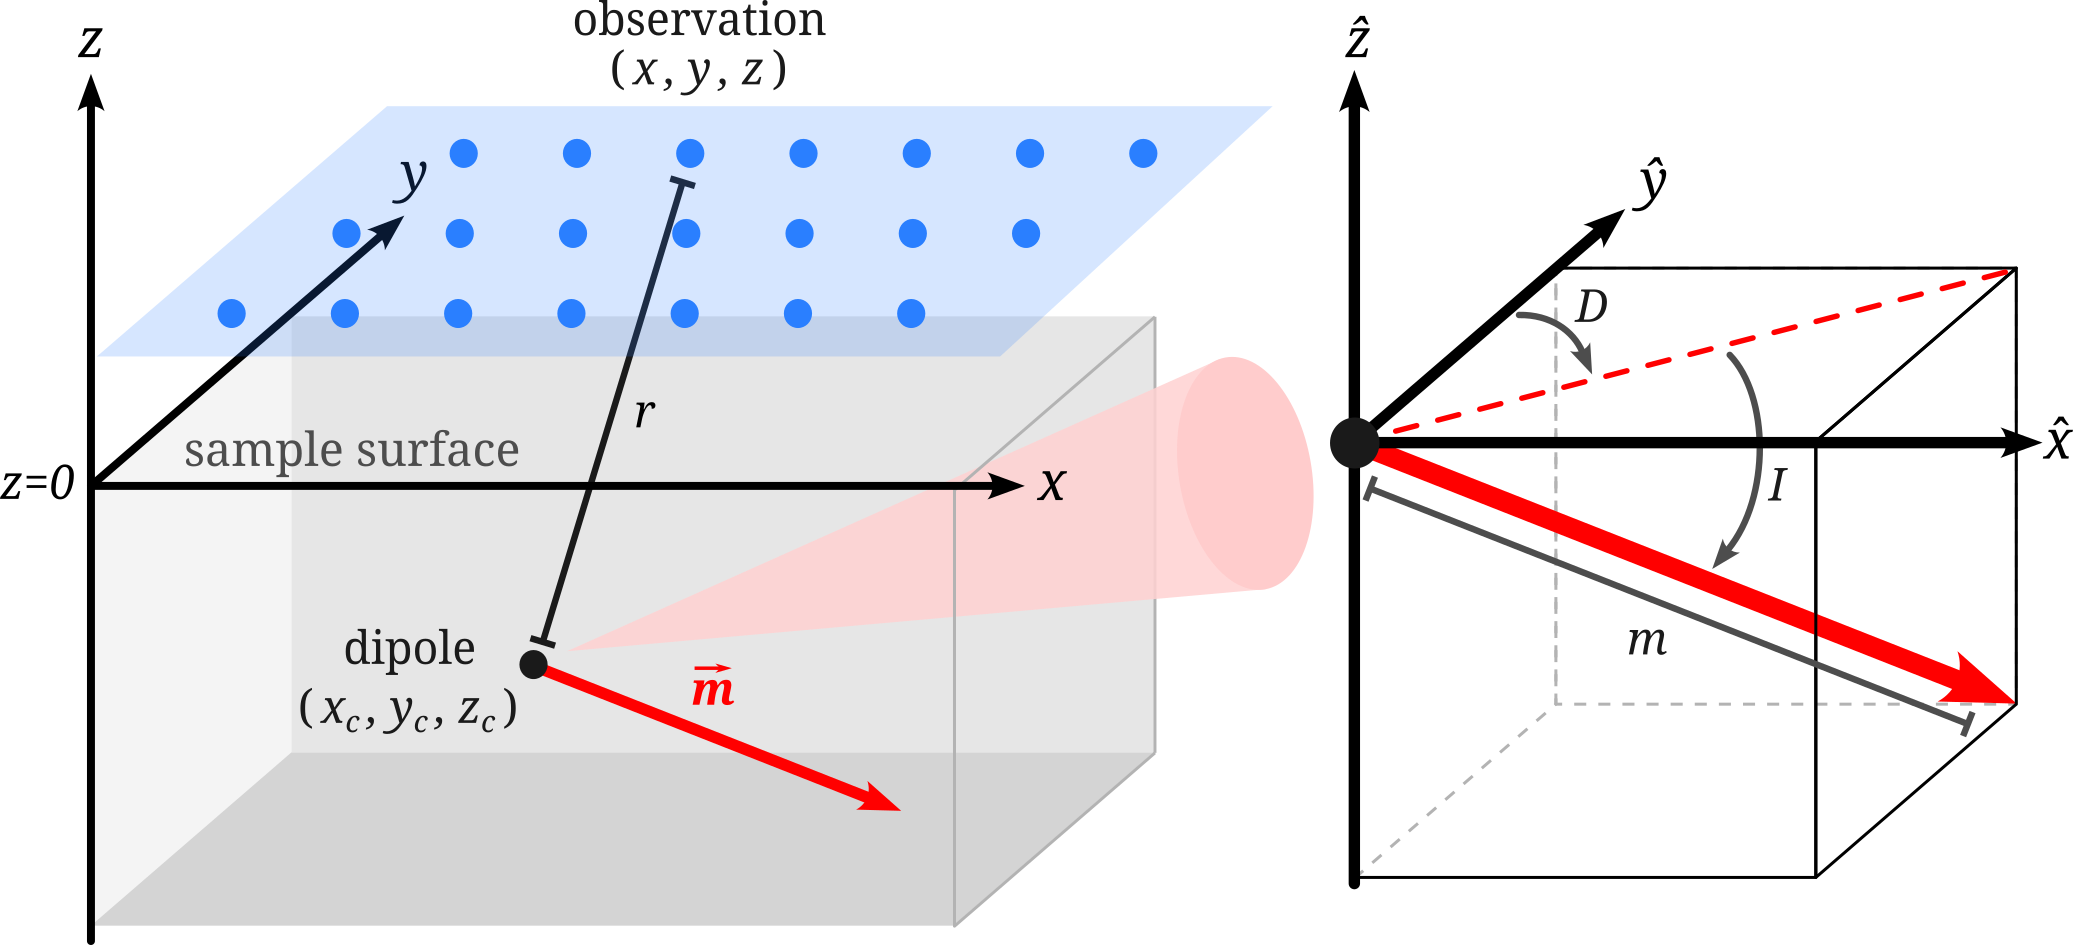
\includegraphics[width=\linewidth]{micromag-euler-dipole/figures/coordinate-system-sketch.png}
\caption{
Schematic representation of the coordinates systems and modeling elements.
The left panel shows the $x, y, z$ right-handed coordinate system with $z$
pointing upward and away from the sample. The top surface of the sample defines
the $z=0$ surface. A dipole with dipole moment vector $\mathbf{\vec{m}}$ is
also shown at coordinates $(x_c, y_c, z_c)$. The observation points are located
at regular intervals on an $x-y$ plane at a positive $z$ separation from the
sample surface. The right panel zooms in on the dipole and shows the dipole
moment vector expressed in terms of inclination ($I$, positive downwards),
declination ($D$, angle with the $\hat{y}$ direction), and moment magnitude $m
= \|\mathbf{m}\|$.
}
\label{fig_coordinate_systems}
\end{figure}

Euler Deconvolution is formulated as a least-squares inversion of Euler's
homogeneity equation

\begin{equation}
\label{eq_euler_homogeneity}
(x - x_c)\partial_x f
+ (y - y_c)\partial_y f
+ (z - z_c)\partial_z f
= (b - f)\eta
\ ,
\end{equation}

\noindent
in which $(x_c, y_c, z_c)$ are the coordinates of the magnetic field source (Figure~\ref{fig_coordinate_systems}), $b$ is the base level representing a constant shift in the signal, and $\eta$ is the structural index corresponding to the nature of the source \citep{Reid1990}. This equation holds true for simple geometric sources, like spheres, dipoles, and vertical cylinders. Here, we assume that the magnetic particles are small enough and the sensor is far enough away that the sources can be represented by dipoles, yielding an $\eta=3$.

The inversion is performed by rearranging Equation~\ref{eq_euler_homogeneity} into a pseudo-parametric model with parameters $x_c$, $y_c$, $z_c$, and $b$

\begin{equation}
x_c \partial_x f + y_c \partial_y f + z_c \partial_z f + \eta b
=
x \partial_x f + y \partial_y f + z \partial_z f + \eta f
\ .
\end{equation}

Given a set of $N$ observations of the magnetic field as the harmonic function $f$ and its spatial derivatives, we can form the $N \times 4$ system of equations

\begin{equation}
\begin{bmatrix}
  {\partial_x f}_1 & {\partial_y f}_1 & {\partial_z f}_1 & \eta \\
  {\partial_x f}_2 & {\partial_y f}_2 & {\partial_z f}_2 & \eta \\
  \vdots & \vdots & \vdots & \vdots \\
  {\partial_x f}_N & {\partial_y f}_N & {\partial_z f}_N & \eta
\end{bmatrix}
\begin{bmatrix}
  x_c \\ y_c \\ z_c \\ b
\end{bmatrix}
=
\begin{bmatrix}
  x_1 {\partial_x f}_1 + y_1 {\partial_y f}_1 + z_1 {\partial_z f}_1 + \eta f_1 \\
  x_2 {\partial_x f}_2 + y_2 {\partial_y f}_2 + z_2 {\partial_z f}_2 + \eta f_2 \\
  \vdots \\
  x_N {\partial_x f}_N + y_N {\partial_y f}_N + z_N {\partial_z f}_N + \eta f_N \\
\end{bmatrix}
\ .
\end{equation}

In matrix notation, this linear system can be written as

\begin{equation}
\label{eq_euler_forward}
\mathbf{G} \mathbf{p} = \mathbf{h} \ .
\end{equation}

We can arrive at a solution to Equation~\ref{eq_euler_forward} by assuming that the three spatial derivatives of $f$ have negligible error and minimizing the misfit $\phi(\mathbf{p})$ between a pseudo-observation vector $\mathbf{h}^o$ and the predictions $\mathbf{h}$. The least-squares misfit $\phi(\mathbf{p})$ is defined as

\begin{equation}
\label{ZTSuSBbL16}
\phi(\mathbf{p}) = \|\mathbf{h}^o - \mathbf{h}\|^2 = (\mathbf{h}^o - \mathbf{G}\mathbf{p})^T (\mathbf{h}^o - \mathbf{G}\mathbf{p})\ .
\end{equation}

The minimum of $\phi(\mathbf{p})$ is obtained by solving the $4 \times 4$
system of normal equations

\begin{equation}
\mathbf{G}^T \mathbf{G} \mathbf{p} = \mathbf{G}^T \mathbf{h}^o\ .
\end{equation}

The solution vector $\hat{\mathbf{p}}$ provides an estimate of the position
$(x_c, y_c, z_c)$ and base level $b$ for the source located inside of a data
window. Repeating this process for each window produced by the source detection
algorithm will yield the horizontal locations and depths of each magnetic
particle.

\subsection{Magnetic moment inversion}

Once the source's position is known, and assuming it is a dipole, we can apply the method developed by
\citet{Oliveira2015Estimation} to estimate the dipole moment vector
$\mathbf{m}$ of the source. We begin by following
\citet{Oliveira2015Estimation} in formulating the magnetic induction vector
$\mathbf{b}$ of a dipole as

\begin{equation}
\label{eq_vector_dipole_field}
\mathbf{b}
=
\begin{bmatrix}
  b_x \\ b_y \\ b_z
\end{bmatrix}
= \dfrac{\mu_0}{4\pi}
\begin{bmatrix}
    \dfrac{\partial^2}{\partial x \partial x} \dfrac{1}{r}
  & \dfrac{\partial^2}{\partial x \partial y} \dfrac{1}{r}
  & \dfrac{\partial^2}{\partial x \partial z} \dfrac{1}{r}
  \\
    \dfrac{\partial^2}{\partial y \partial x} \dfrac{1}{r}
  & \dfrac{\partial^2}{\partial y \partial y} \dfrac{1}{r}
  & \dfrac{\partial^2}{\partial y \partial z} \dfrac{1}{r}
  \\
  \dfrac{\partial^2}{\partial z \partial x} \dfrac{1}{r}
  & \dfrac{\partial^2}{\partial z \partial y} \dfrac{1}{r}
  & \dfrac{\partial^2}{\partial z \partial z} \dfrac{1}{r}
\end{bmatrix}
\begin{bmatrix}
  m_x \\ m_y \\ m_z
\end{bmatrix}
= \dfrac{\mu_0}{4\pi} \mathbf{M}\,\mathbf{m}
\ ,
\end{equation}

\noindent
in which $r = \sqrt{(x - x_c)^2 + (y - y_c)^2 + (z - z_c)^2}$ is the Cartesian distance between the observation point $(x, y, z)$ and the source $(x_c, y_c, z_c)$ and $\mu_0$ is the vacuum magnetic permeability. Most magnetic microscopes provide measurements of only the vertical component $b_z$, which can be isolated from Equation~\ref{eq_vector_dipole_field} as shown in Equation~\ref{eq_dipole_bz}, which is a similar approach to the uniform model proposed by \cite{Weiss2007}.

\begin{equation}
\label{eq_dipole_bz}
b_z
= \dfrac{\mu_0}{4\pi}
\begin{bmatrix}
\dfrac{\partial^2}{\partial z \partial x} \dfrac{1}{r}
& \dfrac{\partial^2}{\partial z \partial y} \dfrac{1}{r}
& \dfrac{\partial^2}{\partial z \partial z} \dfrac{1}{r}
\end{bmatrix}
\begin{bmatrix}
m_x \\ m_y \\ m_z
\end{bmatrix}
= \dfrac{\mu_0}{4\pi} \mathbf{M_z}\,\mathbf{m}
\ .
\end{equation}

The three second-order derivatives in Equation~\ref{eq_dipole_bz} are

\begin{equation}
\begin{aligned}
\dfrac{\partial^2}{\partial z \partial x} \dfrac{1}{r} &=
\dfrac{3(z - z_c)(x - x_c)}{r^5}\ ,
\\
\dfrac{\partial^2}{\partial z \partial y} \dfrac{1}{r} &=
\dfrac{3(z - z_c)(y - y_c)}{r^5}\ ,
\\
\dfrac{\partial^2}{\partial z \partial z} \dfrac{1}{r} &=
\dfrac{3(z - z_c)^2}{r^5} - \dfrac{1}{r^3}\ .
\end{aligned}
\end{equation}

Given a set of $N$ observations of $b_z$ made inside a window containing a single source, we can form the $N \times 3$ linear equation system

\begin{equation}
\label{CgjOtKLQKT}
\begin{bmatrix}
\dfrac{\mu_0}{4\pi}\dfrac{3(z_1 - z_c)(x_1 - x_c)}{r_1^5}
& \dfrac{\mu_0}{4\pi}\dfrac{3(z_1 - z_c)(y_1 - y_c)}{r_1^5}
& \dfrac{\mu_0}{4\pi}\left(\dfrac{3(z_1 - z_c)^2}{r_1^5} - \dfrac{1}{r_1^3}\right)
\\
\dfrac{\mu_0}{4\pi}\dfrac{3(z_2 - z_c)(x_2 - x_c)}{r_2^5}
& \dfrac{\mu_0}{4\pi}\dfrac{3(z_2 - z_c)(y_2 - y_c)}{r_2^5}
& \dfrac{\mu_0}{4\pi}\left(\dfrac{3(z_2 - z_c)^2}{r_2^5} - \dfrac{1}{r_2^3}\right)
\\
\vdots & \vdots & \vdots
\\
\dfrac{\mu_0}{4\pi}\dfrac{3(z_N - z_c)(x_N - x_c)}{r_N^5}
& \dfrac{\mu_0}{4\pi}\dfrac{3(z_N - z_c)(y_N - y_c)}{r_N^5}
& \dfrac{\mu_0}{4\pi}\left(\dfrac{3(z_N - z_c)^2}{r_N^5} - \dfrac{1}{r_N^3}\right)
\end{bmatrix}
\begin{bmatrix}
m_x \\ m_y \\ m_z
\end{bmatrix}
=
\begin{bmatrix}
{b_z}_1 \\ {b_z}_2 \\ \vdots \\ {b_z}_N
\end{bmatrix}
\ ,
\end{equation}

\noindent
which can also be expressed in matrix form as

\begin{equation}
\label{qdhqM4s9Ln}
\mathbf{A} \mathbf{m} = \mathbf{d} \ .
\end{equation}

As with Euler Deconvolution, we can find a dipole moment vector that best fits
a set of $N$ observations of the vertical component of the magnetic field
$\mathbf{d}^o$ in a least-squares sense by minimizing the misfit function

\begin{equation}
\label{uV9pRVYO4l}
\Gamma (\mathbf{m}) = \| \mathbf{d}^o - \mathbf{d} \|^2 = (\mathbf{d}^o - \mathbf{A}\mathbf{m})^T  (\mathbf{d}^o - \mathbf{A}\mathbf{m})\ .
\end{equation}

\noindent
The dipole moment vector that minimizes $\Gamma (\mathbf{m})$ can be found by
solving the $3 \times 3$ normal equation system

\begin{equation}
\mathbf{A}^T \mathbf{A} \mathbf{m} = \mathbf{A}^T\mathbf{d}^o\ .
\end{equation}

\noindent
The estimated dipole moment vector $\hat{\mathbf{m}}$ can be converted into declination $D$, inclination $I$, and magnitude $m$, which are more intuitive quantities for interpreting paleomagnetic results, like so \citep{Tauxe2018}

\begin{equation}
\label{eq_vector_to_incdec}
\begin{aligned}
I &= -\tan^{-1}\dfrac{m_z}{\sqrt{m_x^2 + m_y^2}} \ , \\
D &= \tan^{-1}\dfrac{m_x}{m_y} \ , \\
m &= \sqrt{m_x^2 + m_y^2 + m_z^2} \ .
\end{aligned}
\end{equation}

\noindent
It is important to note that these are not paleomagnetic declination and inclination angles, but are instead related to the sample coordinate system. To obtain the paleomagnetic direction, the dipole moment vector must be rotated to the sample field orientation prior to the application of Equation~\ref{eq_vector_to_incdec}.

In a micromagnetic survey, or any geophysical survey, measurements are affected by noise caused by experimental errors, equipment inaccuracies, and sensor limitations. This noise will affect the estimated parameter vector $\mathbf{\hat{m}}$, regardless of the method used. Assuming that the noise in the observed data is independent and normally distributed with zero mean and variance ${\sigma_0}^2$, we can estimate the variance of the parameters by propagation of uncertainties. In reality, the data variance  ${\sigma_0}^2$ is rarely known and must be estimated using the $\chi^2$ statistic \citep{Aster2019}

\begin{equation}
\label{eq_chi_square}
\hat{\sigma}_0^2 = {\chi}^2 = \dfrac{\|\mathbf{d}^o - \mathbf{A}\hat{\mathbf{m}}\|^2}{N - 3}\ ,
\end{equation}

\noindent
in which $N - 3$  are the degrees-of-freedom.
The covariance matrix $\mathbf{C}$ of the estimated parameters is then given by \citep{Aster2019}

\begin{equation}
\label{eq_covariance}
\mathbf{C}
=
\hat{\sigma}_0^2 (\mathbf{A}^T\mathbf{A})^{-1}
=
\begin{bmatrix}
\sigma_x^2 & \sigma_{xy} & \sigma_{xz} \\
\sigma_{yx} & \sigma_y^2 & \sigma_{yz} \\
\sigma_{zx} & \sigma_{zy} & \sigma_z^2
\end{bmatrix}
\ .
\end{equation}

\noindent
From the main diagonal of $\mathbf{C}$, we can obtain the variances of the
estimated declination $\sigma_D^2$, inclination $\sigma_I^2$, and magnitude $\sigma_m^2$
by the propagation of uncertainties from Equation~\ref{eq_vector_to_incdec}

\begin{equation}
\label{eq_variances}
\begin{aligned}
\sigma_D^2 &= \dfrac{m_y^2\sigma_x^2 + m_x^2\sigma_y^2}{\left(m_x^2 + m_y^2\right)^2} \ , \\
\sigma_I^2 &= \dfrac{m_x^2 m_z^2 \sigma_x^2 + m_y^2 m_z^2 \sigma_y^2 + \left(m_x^2 + m_y^2\right)^2\sigma_z^2}{\left(m_x^2 + m_y^2\right) m^4} \ , \\
\sigma_m^2 &= \dfrac{m_x^2\sigma_x^2 + m_y^2\sigma_y^2 + m_z^2\sigma_z^2}{m^2} \ .
\end{aligned}
\end{equation}

\noindent
These variances reflect the sensitivity of the estimated dipole moment to random noise in the magnetic field observations. However, they do not capture other, often larger, sources of uncertainty like systematic errors in the observations, data positioning errors, and the validity of the dipolar approximation. Therefore, we recommend that these estimated variances be treated with caution and should not be interpreted as ``the degree of certainty that the estimated values are the true values''.

Parameters retrieved during inversion procedures may not always explain the observed data perfectly.
Hence, it is necessary to evaluate how well the predicted data is able to fit the observed data.
When evaluating the goodness of fit of inversions of magnetic microscopy data, \citet{Fu2020} apply a ``dipolarity parameter'' ($D$).
We note that $D$ is equivalent to the coefficient of determination

\begin{equation}
\label{eq_r2}
R^2 = 1 - \dfrac{\|\mathbf{d}^o - \mathbf{A}\hat{\mathbf{m}}\|^2}{\|\mathbf{d}^o - \bar{b}_z^o\|^2}\ ,
\end{equation}

\noindent
in which $\bar{b}_z^o$ is the mean of the observed data.
$R^2$ has a maximum value of 1, which indicates a perfect fit of the data.
Values close to 1 can therefore be interpreted to mean that a simple dipole model is able to explain the observed data.
On the other hand, low values of $R^2$ indicate that the dipole model is not able to explain the observed data.

\citet{CortesOrtuno2021} use the ``signal-to-noise ratio'' (SNR) to evaluate the goodness of fit.
Here, we define the SNR in a logarithmic decibel scale to make it independent of the scale of the data

\begin{equation}
\label{eq_snr}
\text{SNR} = 10 \log_{10}\dfrac{\sigma^2_d}{\sigma^2_r}\ ,
\end{equation}

\noindent
in which $\sigma^2_d$ is the variance of the observed data and $\sigma^2_r$ is the variance of the residuals $\mathbf{r} = \mathbf{d}^o - \mathbf{A}\hat{\mathbf{m}}$.
The SNR is the trade-off between the signal and its associated noise, which we approximate by the inversion residuals.
The higher the SNR values (in decibels), the better the fit to the observed data.
For a signal to be ``visible'', \citet{Strum2014} suggest that $\text{SNR} \ge 3$, which means the signal is at least three times stronger than the noise.
Here, we use both $R^2$ and SNR as criteria for filtering out unreliable estimates from our dipole moment inversions.


%%%%%%%%%%%%%%%%%%%%%%%%%%%%%%%%%%%%%%%%%%%%%%%%%%%%%%%%%%%%%%%%%%%%%%%%%%%%%%%
\section{Application to synthetic data}

We first applied our inversion workflow to four sets of synthetic data to evaluate its strengths and limitations.
The datasets are produced by different models of varying complexity which were designed to assess different aspects of the method.

\begin{enumerate}
\item \textbf{Method validation:}
The first model is composed of a set of four dipoles with similar dipole moments amplitudes, but different inclinations and declinations.
The synthetic data consists of the vertical magnetic field ($b_z$) derived from this model and contaminated by pseudo-random high-frequency noise.
The purpose of this simple model is to investigate the efficiency of the combination of the source detection method, Euler deconvolution, and the dipole moment inversion under ideal circumstances, thus serving as a validation of the methodology.

\item \textbf{Applicability to non-dipolar sources:}
The second model simulates a hundred sources with both dipolar and non-dipolar magnetic moments.
Their vertical magnetic field ($b_z$) is calculated at different sensor-source distances
and is also contaminated with pseudo-random high-frequency noise.
This model is used to assess the ability of the algorithm to deal with strong non-dipolar sources.

\item \textbf{Applicability to more complex scenarios:}
The third model is inspired on typical speleothem datasets.
It contains 103 dipoles with different dipole moment magnitudes, having inclinations and declinations clustered around two stable directions.
The magnetic field generated from these sources is corrupted by both low and high-frequency noise.
The complexity of this synthetic data seeks to more faithfully emulate real magnetic microscopy data.

\item \textbf{Applicability to different grain concentration scenarios:}
The fourth model assesses the algorithm's capability to detect magnetic sources in samples with different magnetic particle concentrations. Several scenario tests were conducted, with progressively increasing magnetic grain concentrations. In parallel with this approach, two dipolar sources were gradually separated, also at different sensor heights, until the algorithm could effectively distinguish the signals from both sources. This additional modeling provides insights into the algorithm's performance in scenarios where magnetic sources are closely spaced, complementing the modeling with higher particle density.

\end{enumerate}

\subsection{Method validation}

\begin{figure}[tb!]
  \centering
  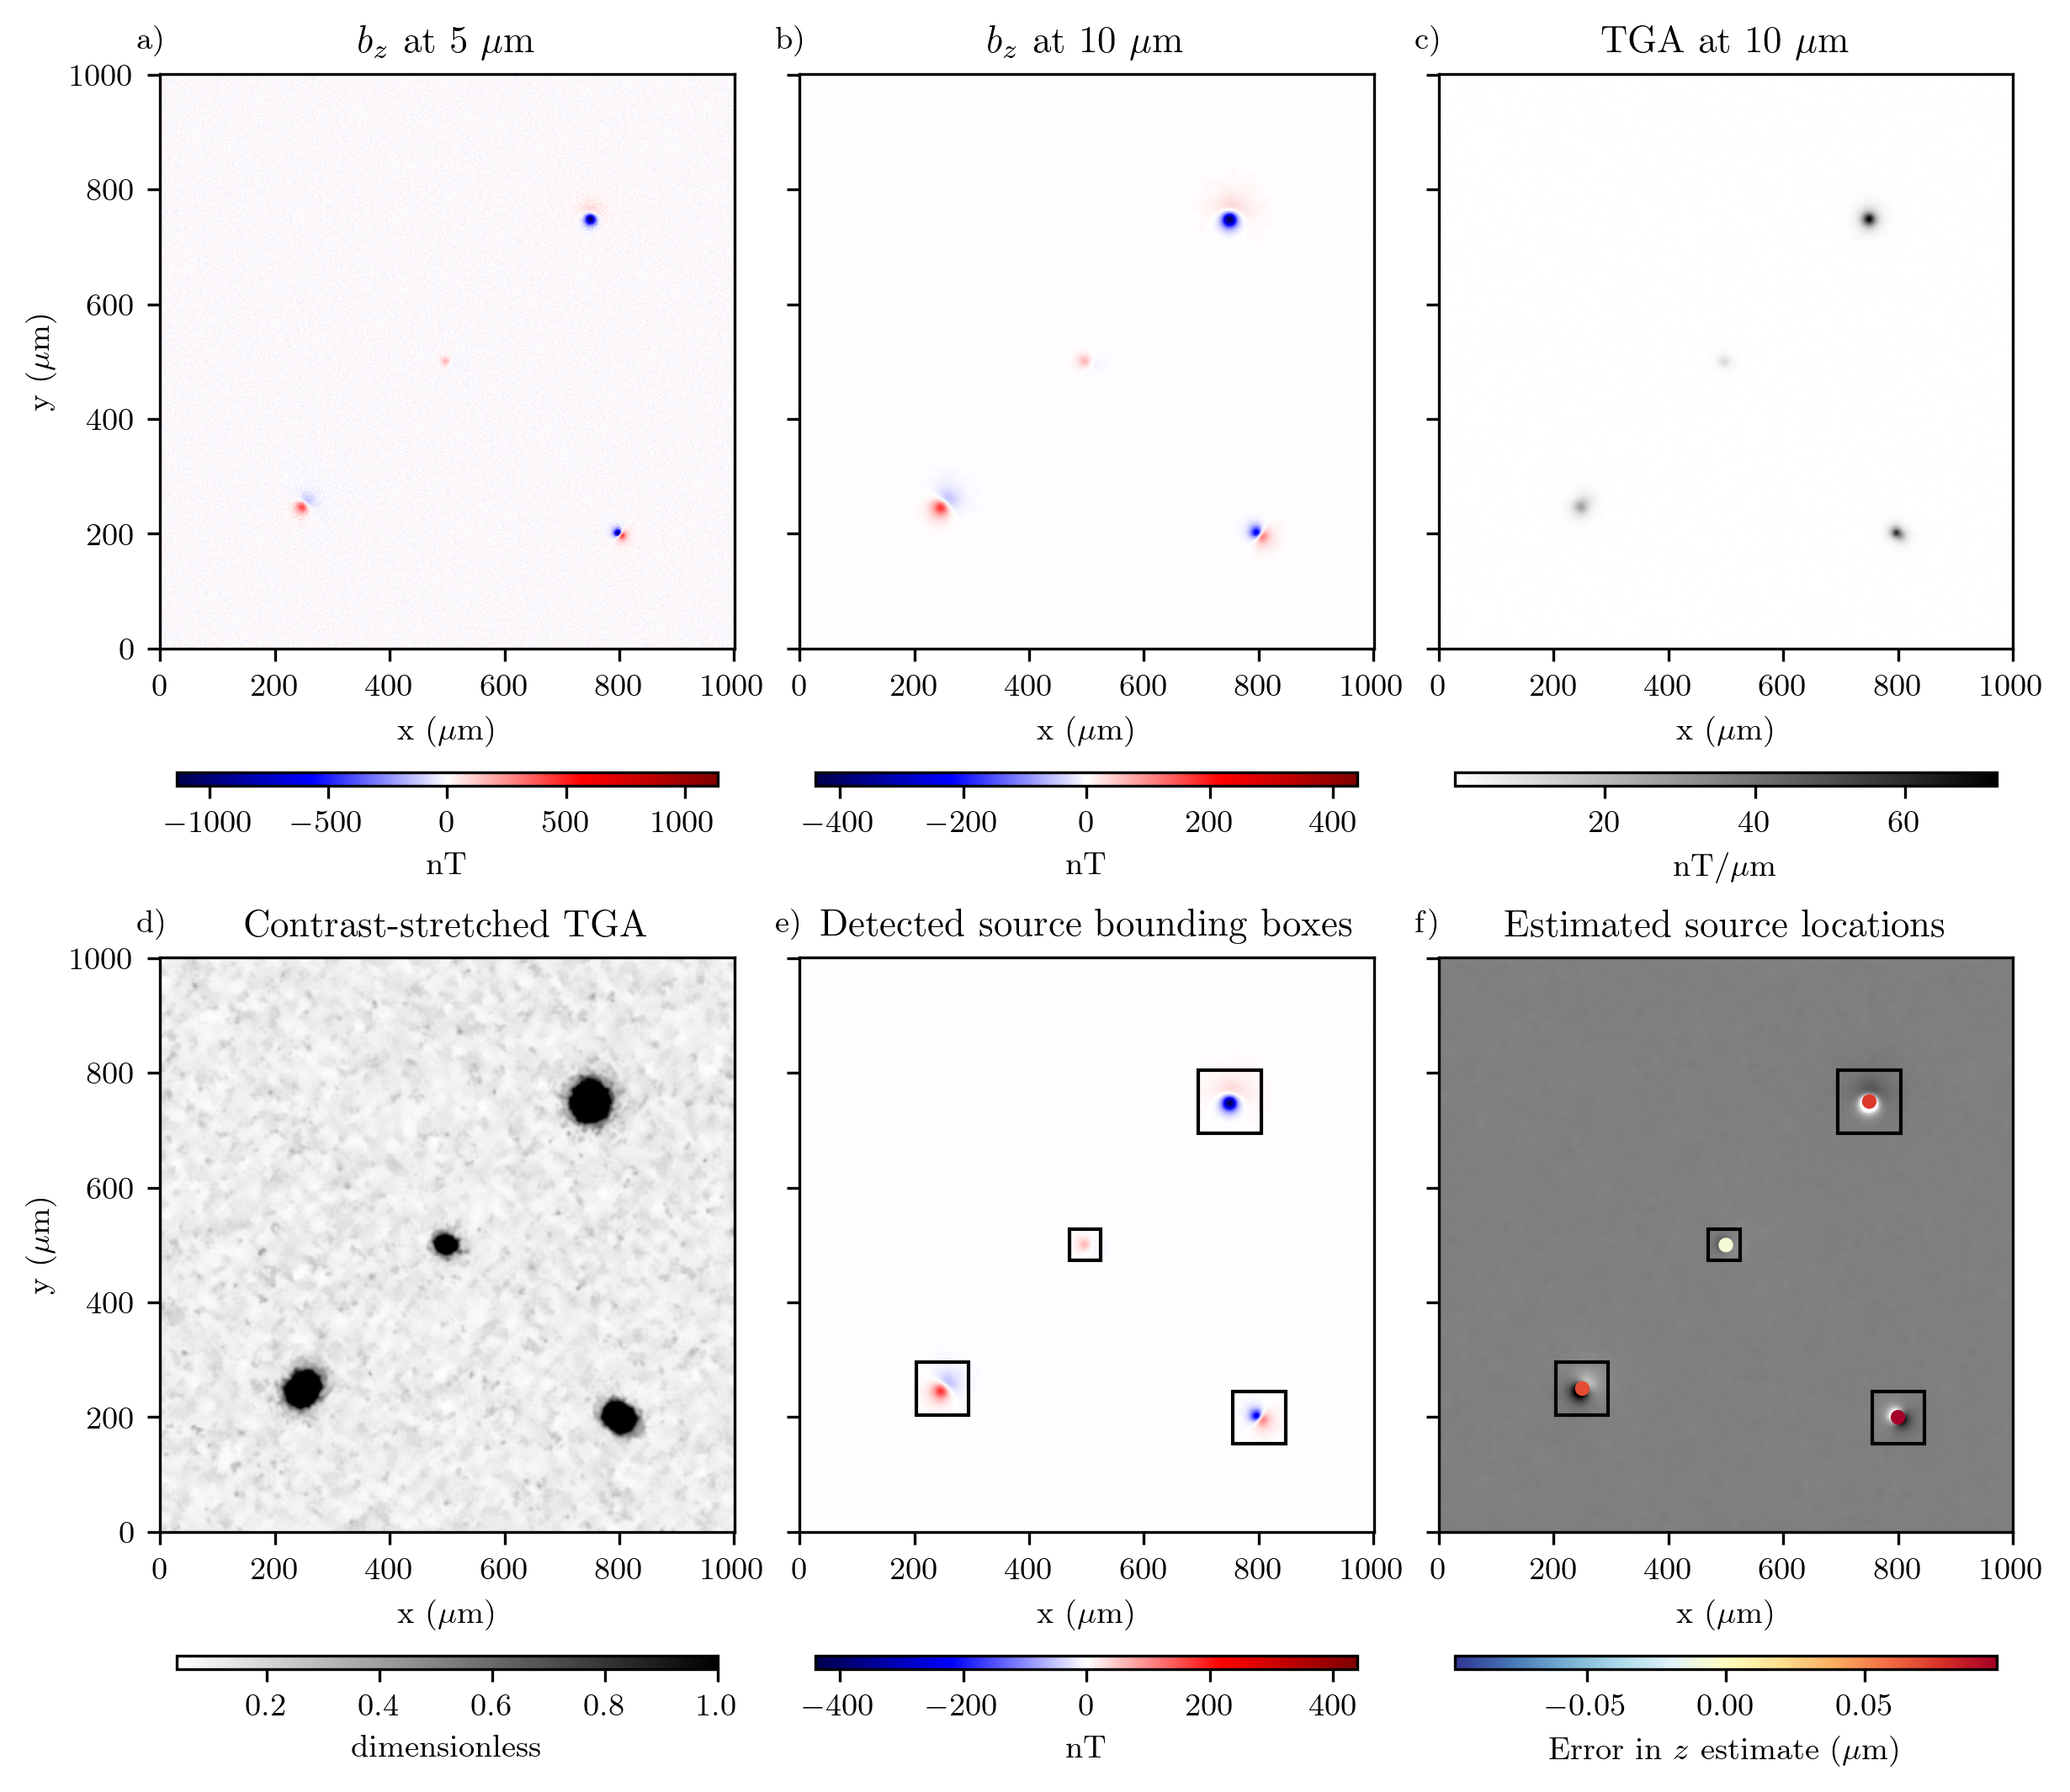
\includegraphics[width=1\linewidth]{micromag-euler-dipole/figures/simple-synthetic-data.png}
  \caption{
    Simple synthetic data and the various processing steps performed prior to the dipole moment inversion.
    a) The synthetic noise-corrupted $b_z$ observations at
    $z = \qty{5}{\micro\meter}$ due to four dipolar sources with different
    depths and dipole moment vectors
    (see Table~\ref{tab_synthetic_simple_results}).
    b) The upward-continued data to $z = \qty{10}{\micro\meter}$ showing
    attenuated short-wavelength noise.
    c) The total gradient amplitude (TGA) calculated from the
    upward-continued data, which is able to concentrate the signal on top
    of each dipolar source.
    d) The contrast-stretched TGA, highlighting the signal of all four
    sources, including the weak central source.
    e) The detected source bounding boxes (black squares) that correctly
    identify the signal of all four sources.
    f) The estimated source locations (colored circles) from Euler
    deconvolution of the upward-continued data inside each bounding box.
    The color represents the difference between the true and the estimated
    $z$ coordinates.
  }
  \label{fig_synthetic_simple_data}
\end{figure}

Figure~\ref{fig_synthetic_simple_data}a shows the vertical component of the magnetic field $b_z$ over a synthetic rock section containing four dipolar sources.
The map covers a surface of $\qty{1000}{\um} \times \qty{1000}{\um}$, with data points in a regular grid with approximately \qty{1}{\um} spacing ($N = 10^6$ observations) obtained at a sensor-sample distance of \qty{5}{\um}.
The magnetic field data are contaminated with pseudo-random Gaussian noise with zero mean and \qty{20}{\nano\tesla} standard deviation.

We first applied an upward continuation filter (Figure~\ref{fig_synthetic_simple_data}b) to smooth out the high-frequency noise \citep{Blakely1996}.
This is important because noise strongly affects the first derivatives of the field, which are required for the source detection algorithm and the Euler deconvolution.
Then, we calculated the total gradient amplitude (Figure~\ref{fig_synthetic_simple_data}c), which was subjected to contrast stretching to highlight the weaker intensity sources as much as possible (Figure~\ref{fig_synthetic_simple_data}d).
Subsequently, we applied the blob detection algorithm to the contrast-stretched total gradient amplitude to obtain the position of the data windows for each source (Figure~\ref{fig_synthetic_simple_data}e).
Euler deconvolution was then performed for each data window identified by assuming a structural index $\eta = 3$ of a point source, therefore obtaining the Cartesian coordinates (Figure~\ref{fig_synthetic_simple_data}f) of each source. For comparison, Table~\ref{tab_synthetic_simple_results} shows the true and estimated values of the source coordinates.

\begin{table}[tb!]
  \begin{center}
    \small
    
\begin{tabular}{ r c c c l l l } 
  \toprule
  & \multicolumn{3}{c}{Position} & \multicolumn{3}{c}{Dipole moment} \\
  & $x_c$ ($\mu$m) & $y_c$ ($\mu$m) & $z_c$ ($\mu$m) & $I$ (\textdegree) & $D$ (\textdegree) & $m$ (A.m²) \\
  \midrule
  true & 800.00 & 200.00 & -3.50 & 22.00 & 125.00 & 5.000e-15 \\
  estimated & 799.91 & 199.94 & -3.40 & 22.08 ± 0.01 & 125.52 ± 0.02 & 4.921e-15 ± 1.4e-18 \\
  true & 750.00 & 750.00 & -8.50 & 62.00 & 10.00 & 1.500e-14 \\
  estimated & 749.98 & 749.99 & -8.43 & 62.00 ± 0.01 & 9.30 ± 0.02 & 1.486e-14 ± 1.8e-18 \\
  true & 250.00 & 250.00 & -10.00 & -30.00 & -140.00 & 1.000e-14 \\
  estimated & 250.03 & 249.89 & -9.93 & -30.32 ± 0.01 & -139.70 ± 0.02 & 9.966e-15 ± 2.6e-18 \\
  true & 500.00 & 500.00 & -7.75 & -50.00 & -70.00 & 2.000e-15 \\
  estimated & 500.07 & 499.95 & -7.76 & -48.66 ± 0.05 & -70.36 ± 0.09 & 2.000e-15 ± 1.8e-18 \\
  \bottomrule
\end{tabular}

  \end{center}
  \caption{
    True and estimated source positions and dipole moments for the method validation test through a simple synthetic data application.
  }
  \label{tab_synthetic_simple_results}
\end{table}

\begin{figure}[tb!]
  \centering
  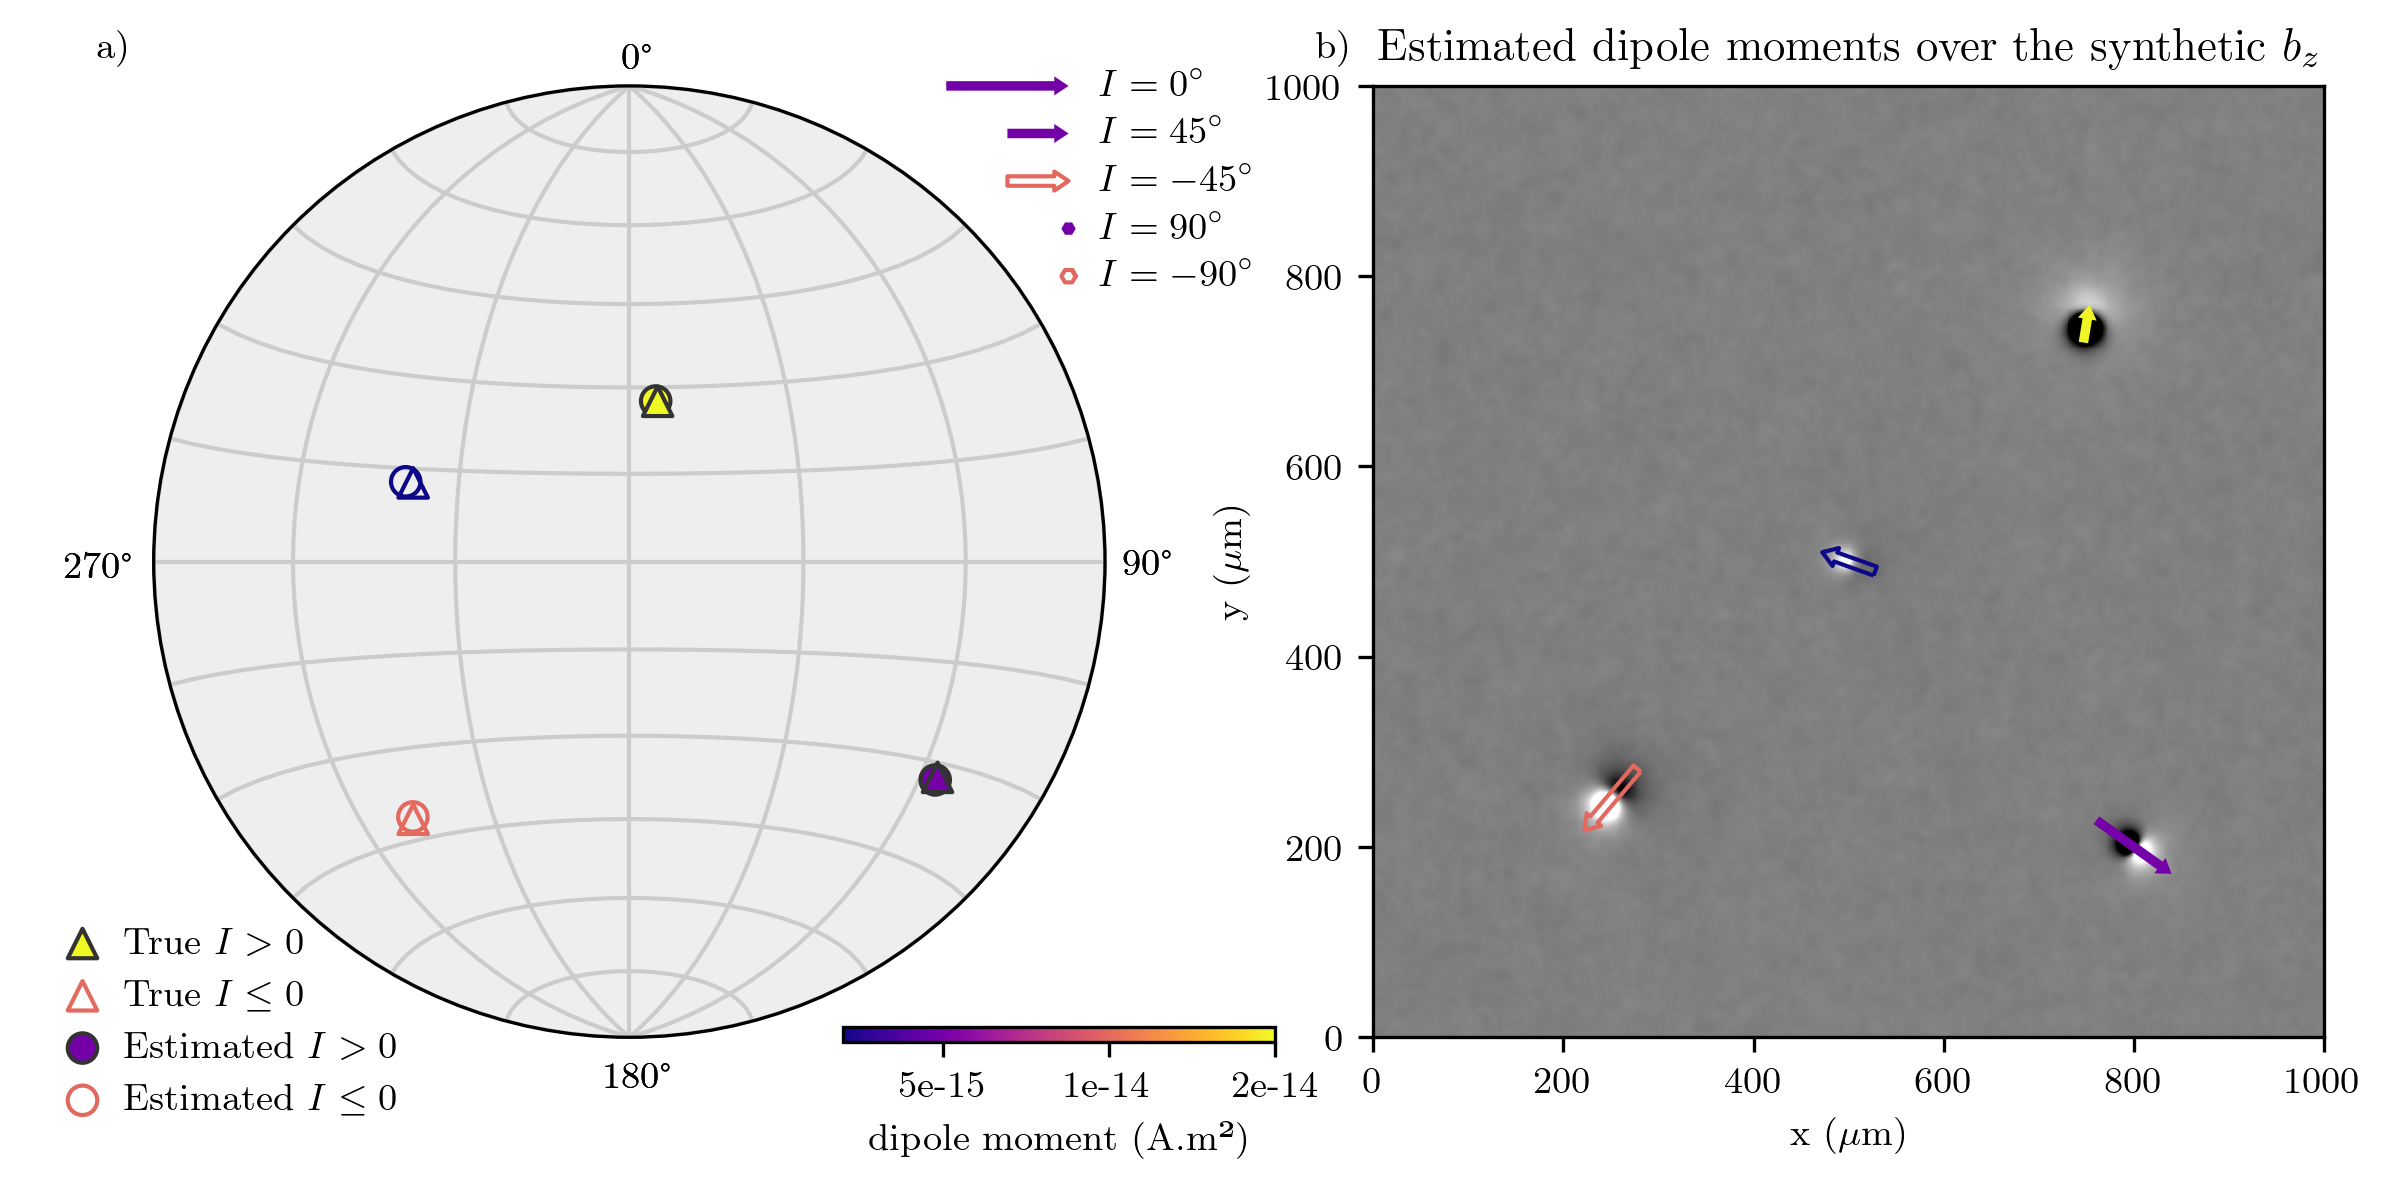
\includegraphics[width=\linewidth]{micromag-euler-dipole/figures/simple-synthetic-dipole-moment.png}
  \caption{
    Comparison of true and estimated dipole moments for the method validation test through a simple synthetic data application.
    a) Stereonet showing the true (triangles) and estimated (circles) dipole moments.
    The colors are mapped to the dipole moment amplitude.
    b) Grayscale map of the synthetic $b_z$ overlaid by the estimated dipole moment vectors.
    The vector locations were derived from the Euler deconvolution results, their size is inversely proportional to the inclination $I$, their direction represents the declination $D$, and their colors are mapped to the dipole moment amplitude using the same colorscale as the stereonet.
    In both graphs, solid symbols represent positive inclination while hollow symbols represent negative inclination.
  }
  \label{fig_synthetic_simple_results}
\end{figure}

The positions of each source obtained with Euler deconvolution were then used as input for the dipole moment inversion.
The estimated dipole moment vectors are shown in Figure~\ref{fig_synthetic_simple_results}.
Figure~\ref{fig_synthetic_simple_results}a shows the estimated dipole moment, along with the corresponding true values, as a stereonet for better comparison of the true and estimated vector directions.
Figure~\ref{fig_synthetic_simple_results}b shows the estimated dipole moments overlaid on a map of the synthetic $b_z$ to demonstrate the ability of our method to estimate a spatial distribution of dipole moments.
For comparison, Table~\ref{tab_synthetic_simple_results} also shows the true and estimated dipole moments as well as their corresponding standard deviations obtained using Equations~\ref{eq_chi_square}-\ref{eq_variances}.



\subsection{Applicability to non-dipolar sources}

Typically, when conducting magnetic field measurements with a large distance between the sensor and the magnetic anomaly source, higher-order non-dipole magnetization components such as quadrupoles and octupoles can be disregarded because of the strong attenuation with distance of the magnetic fields.
However, in magnetic microscopy, where the sensor is positioned only a few microns from the sample, these higher-order components might be detected.
This phenomenon is observed in paleomagnetic studies on particles with a PSD domain state, where magnetization is non-uniform throughout the grain.
To assess the attenuation of these non-dipolar components and the applicability of our method, we conducted a simulation on particles with more complex magnetization at varying sensor-sample distances.

To simulate particles with non-dipolar magnetization components, we specified a spherical volume with a radius of approximately \qty{1}{\um}.
Within this volume, we added 200 dipolar particles with varying dipole moment directions and amplitudes.
These directions were generated randomly, following a normal distribution centered on the direction $D=\ang{90}$ and $I=\ang{0}$ and with a standard deviation of \ang{10}.
The dipole moment amplitudes were sampled by a normal distribution with mean $\qty{e-14}{\ampere\m\squared}$ and standard deviation $\qty{5e-14}{\ampere\m\squared}$.
We also randomly generated spatial positions around a central position of $x_c=\qty{25}{\um}$, $y_c=\qty{25}{\um}$, and $z_c=\qty{-1}{\um}$ with a standard deviation of \qty{0.65}{\um}.
The bulk magnetization of the non-dipolar particle is the vector sum of the dipole moments of each dipole.
The centroid of the spherical volume is defined by the average of the $x_c$, $y_c$, and $z_c$ positions of each dipole.
The synthetic vertical magnetic field $b_z$ of the non-dipolar source was calculated on regular grids with \qty{0.5}{\um} spacing.
Each grid was located at a different sensor-sample distance $z$, varying between \qty{1}{\um} and \qty{10}{\um} in \qty{0.5}{\um} increments.
The synthetic data were corrupted by pseudo-random Gaussian noise of mean \qty{0}{\nano\tesla} and a standard deviation of \qty{20}{\nano\tesla}.
For each data grid generated, we performed Euler deconvolution to estimate the source position and subsequently inverted the data for the dipole moment.
At each step, we recorded the inversion $R^2$ value and the differences between the estimated position and dipole moment and the true centroid and bulk magnetization of the spherical particle.

Figure~\ref{non-dipolarity-synthetic-data} shows the synthetic $b_z$ of an example non-dipolar particle at variable source-sample distances.
When the particle is close to the sensor (\qtyrange{1}{3}{\um}), the observed field is strongly non-dipolar (Figure~\ref{non-dipolarity-synthetic-data}a-b) and the dipole moment inversion produces low $R^2$ values.
As the distance increases, the magnetic field is attenuated, particularly the non-dipolar components which decay more rapidly than the dipolar component.
This results in an increase in $R^2$ (Figure~\ref{non-dipolarity-synthetic-data}c-d).
At distances above \qty{5}{\um}, there is practically only the contribution of the dipolar component, causing $R^2$ to approach its maximum value of 1 (Figure~\ref{non-dipolarity-synthetic-data}e-f).

\begin{figure}[tb!]
  \centering
  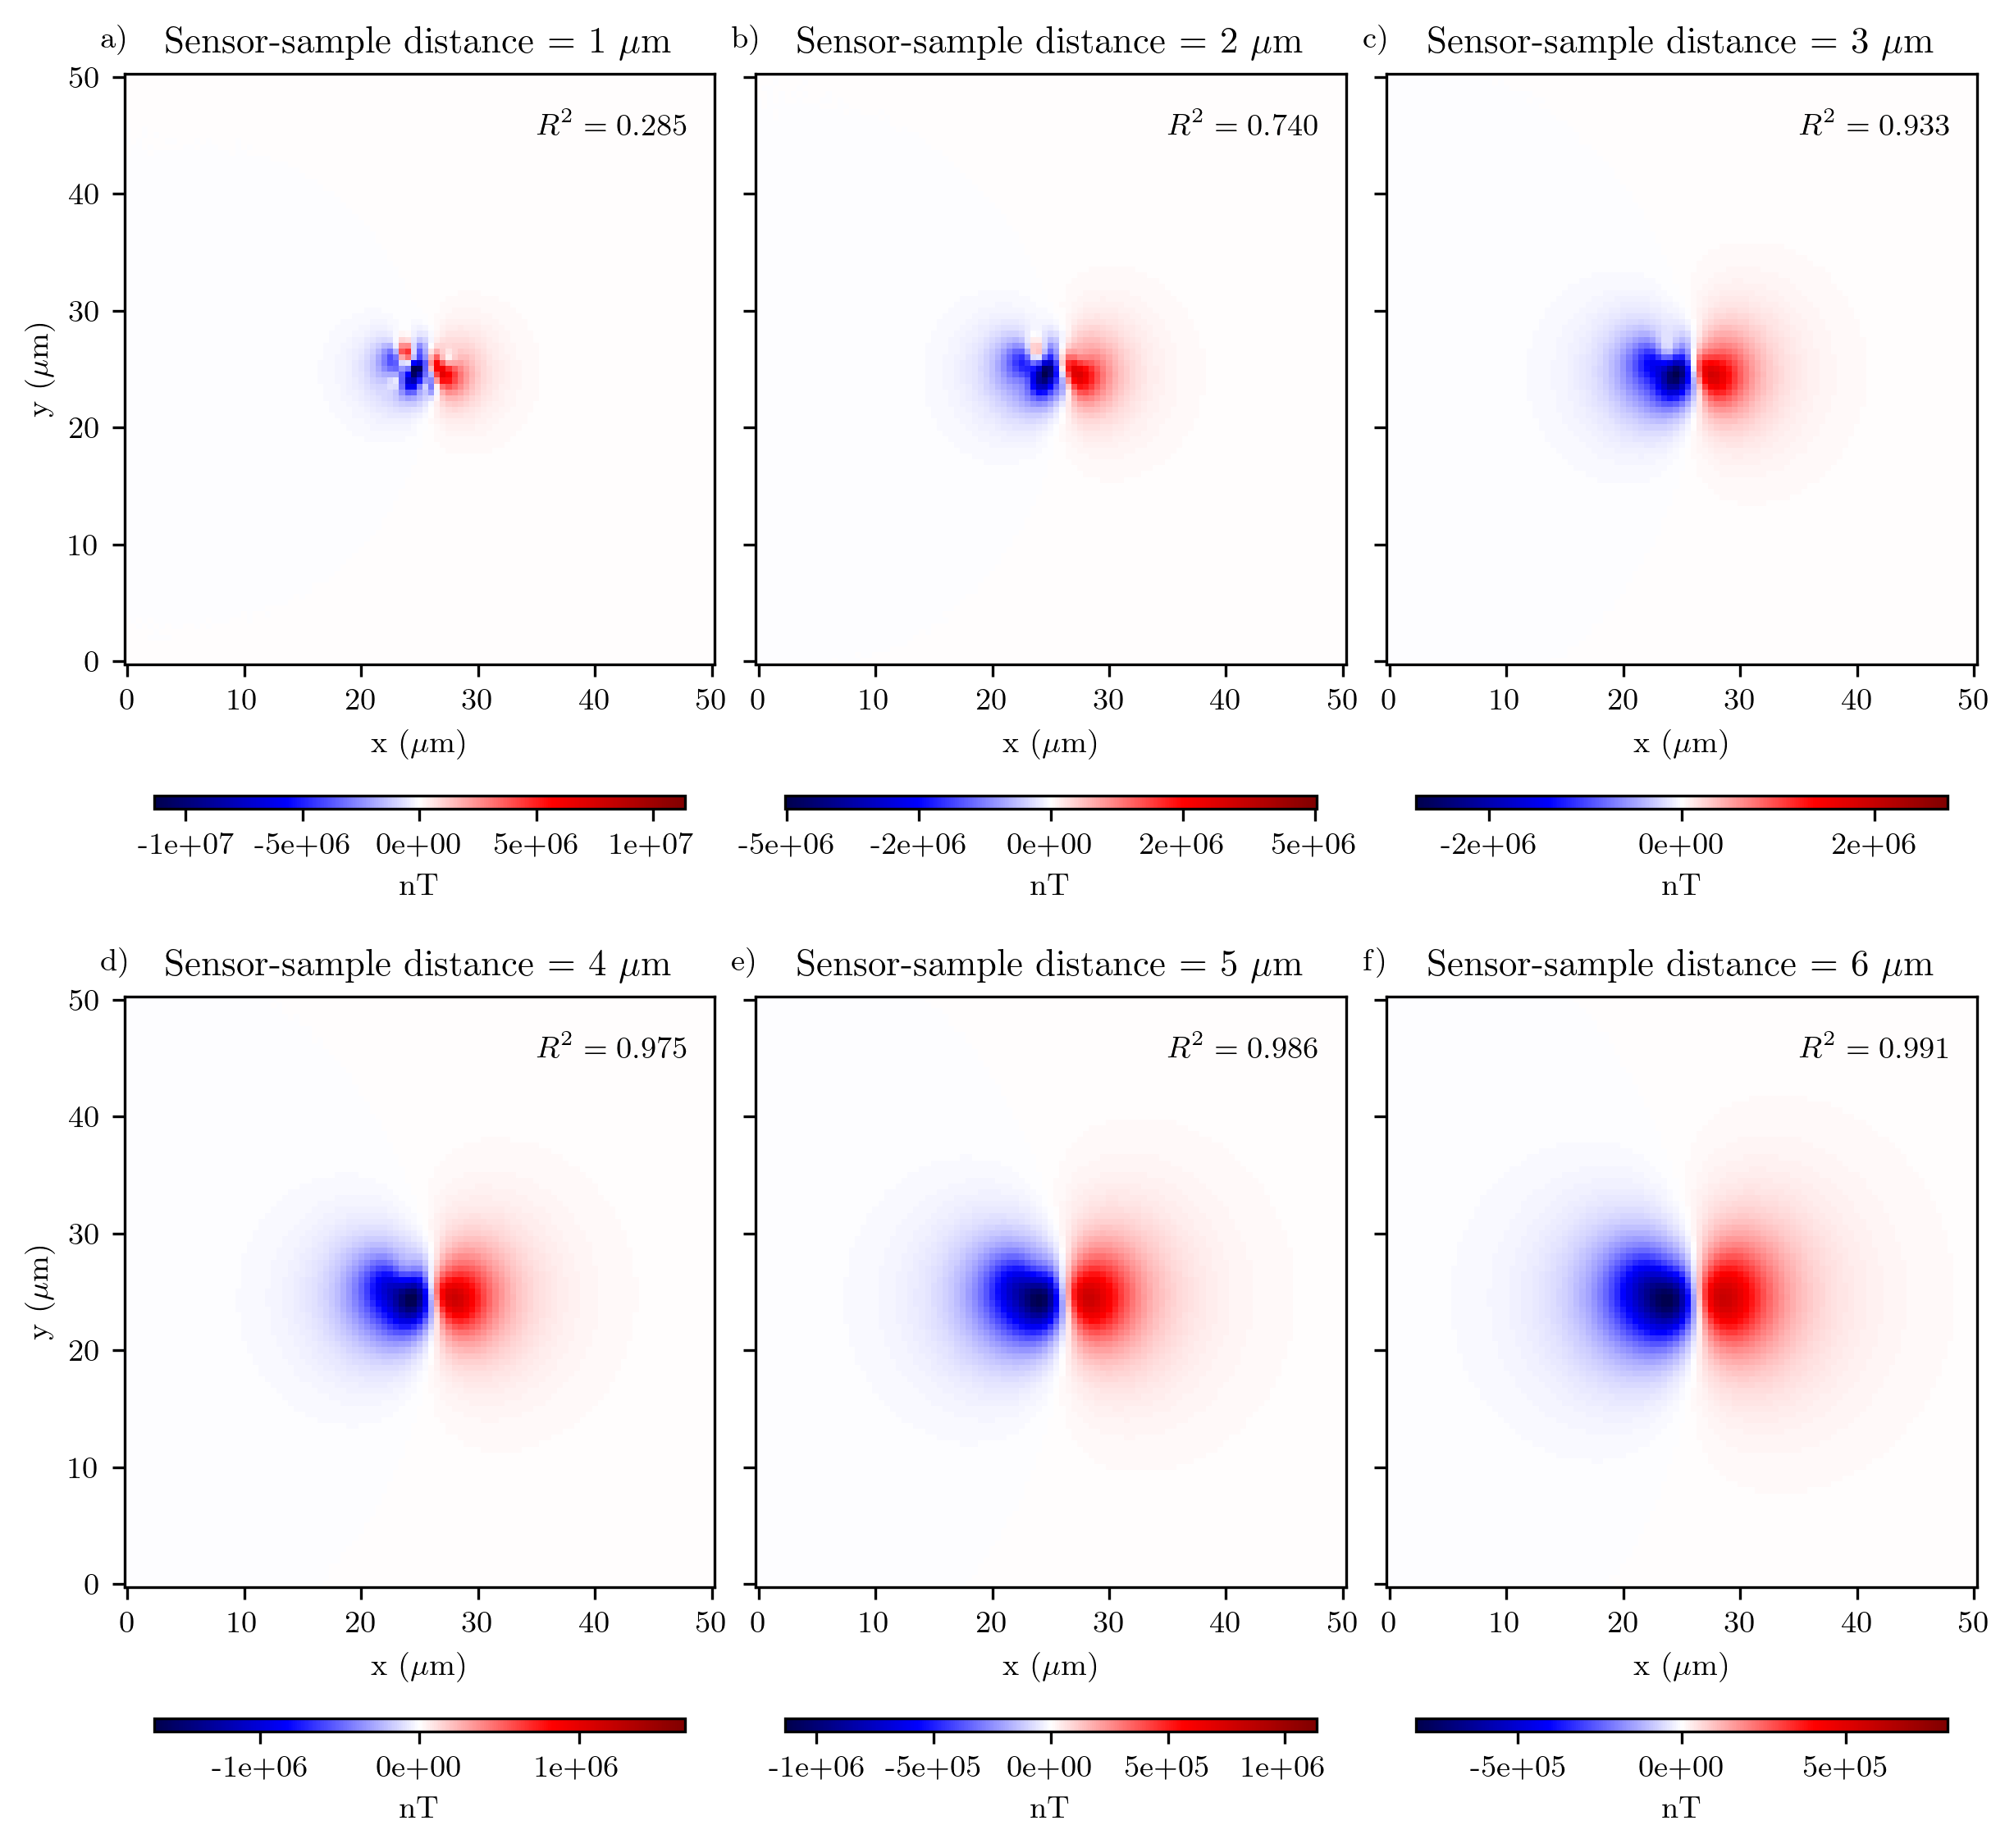
\includegraphics[width=1\linewidth]{micromag-euler-dipole/figures/non-dipolarity-synthetic.png}
  \caption{Caption: Simulated magnetic microscopy data for a spherical source with both dipolar and non-dipolar magnetic components. The distance from the sensor varies from 1 µm to 6 µm (a-f).}
  \label{non-dipolarity-synthetic-data}
\end{figure}

We replicated the particle generation procedure 100 times with variations in the randomness of magnetization and point particle positions. Subsequently, the Cartesian position of the spherical particle was estimated using ED, and the magnetization parameters were determined by inverting the magnetic field data. The effectiveness of position recovery was measured by comparing the centroid of the spherical volume with the solution of the Euler deconvolution for $x_c$, $y_c$, and $z_c$ (Figure~\ref{non-dipolarity-synthetic-data-positioning}a, b, and c, respectively). As shown in Figure~\ref{non-dipolarity-synthetic-data-positioning}, ED estimates the positions of particles with more complex magnetization well, especially for sensor-source distances greater than 5 µm, where the median of the distributions is centered at zero. However, when the sensor-source distance is small enough to emphasize the contribution from higher-order components, a lower degree of dipolarity is observed as expressed by lower values of $R^2$ (Figure~\ref{non-dipolarity-synthetic-data-inversion}a). Consequently, in these cases, there are higher errors in the estimation of the direction of magnetization (Figure~\ref{non-dipolarity-synthetic-data-inversion}b) and in the magnetic moment's intensity (Figure~\ref{non-dipolarity-synthetic-data-inversion}c), which were expected since the inversion considers only the dipolar component. However, dipolarity significantly increases as the sensor-to-sample distance increases, while errors in direction and magnetic moment decrease significantly (Figure~\ref{non-dipolarity-synthetic-data-inversion}).

\begin{figure}[tb!]
  \centering
  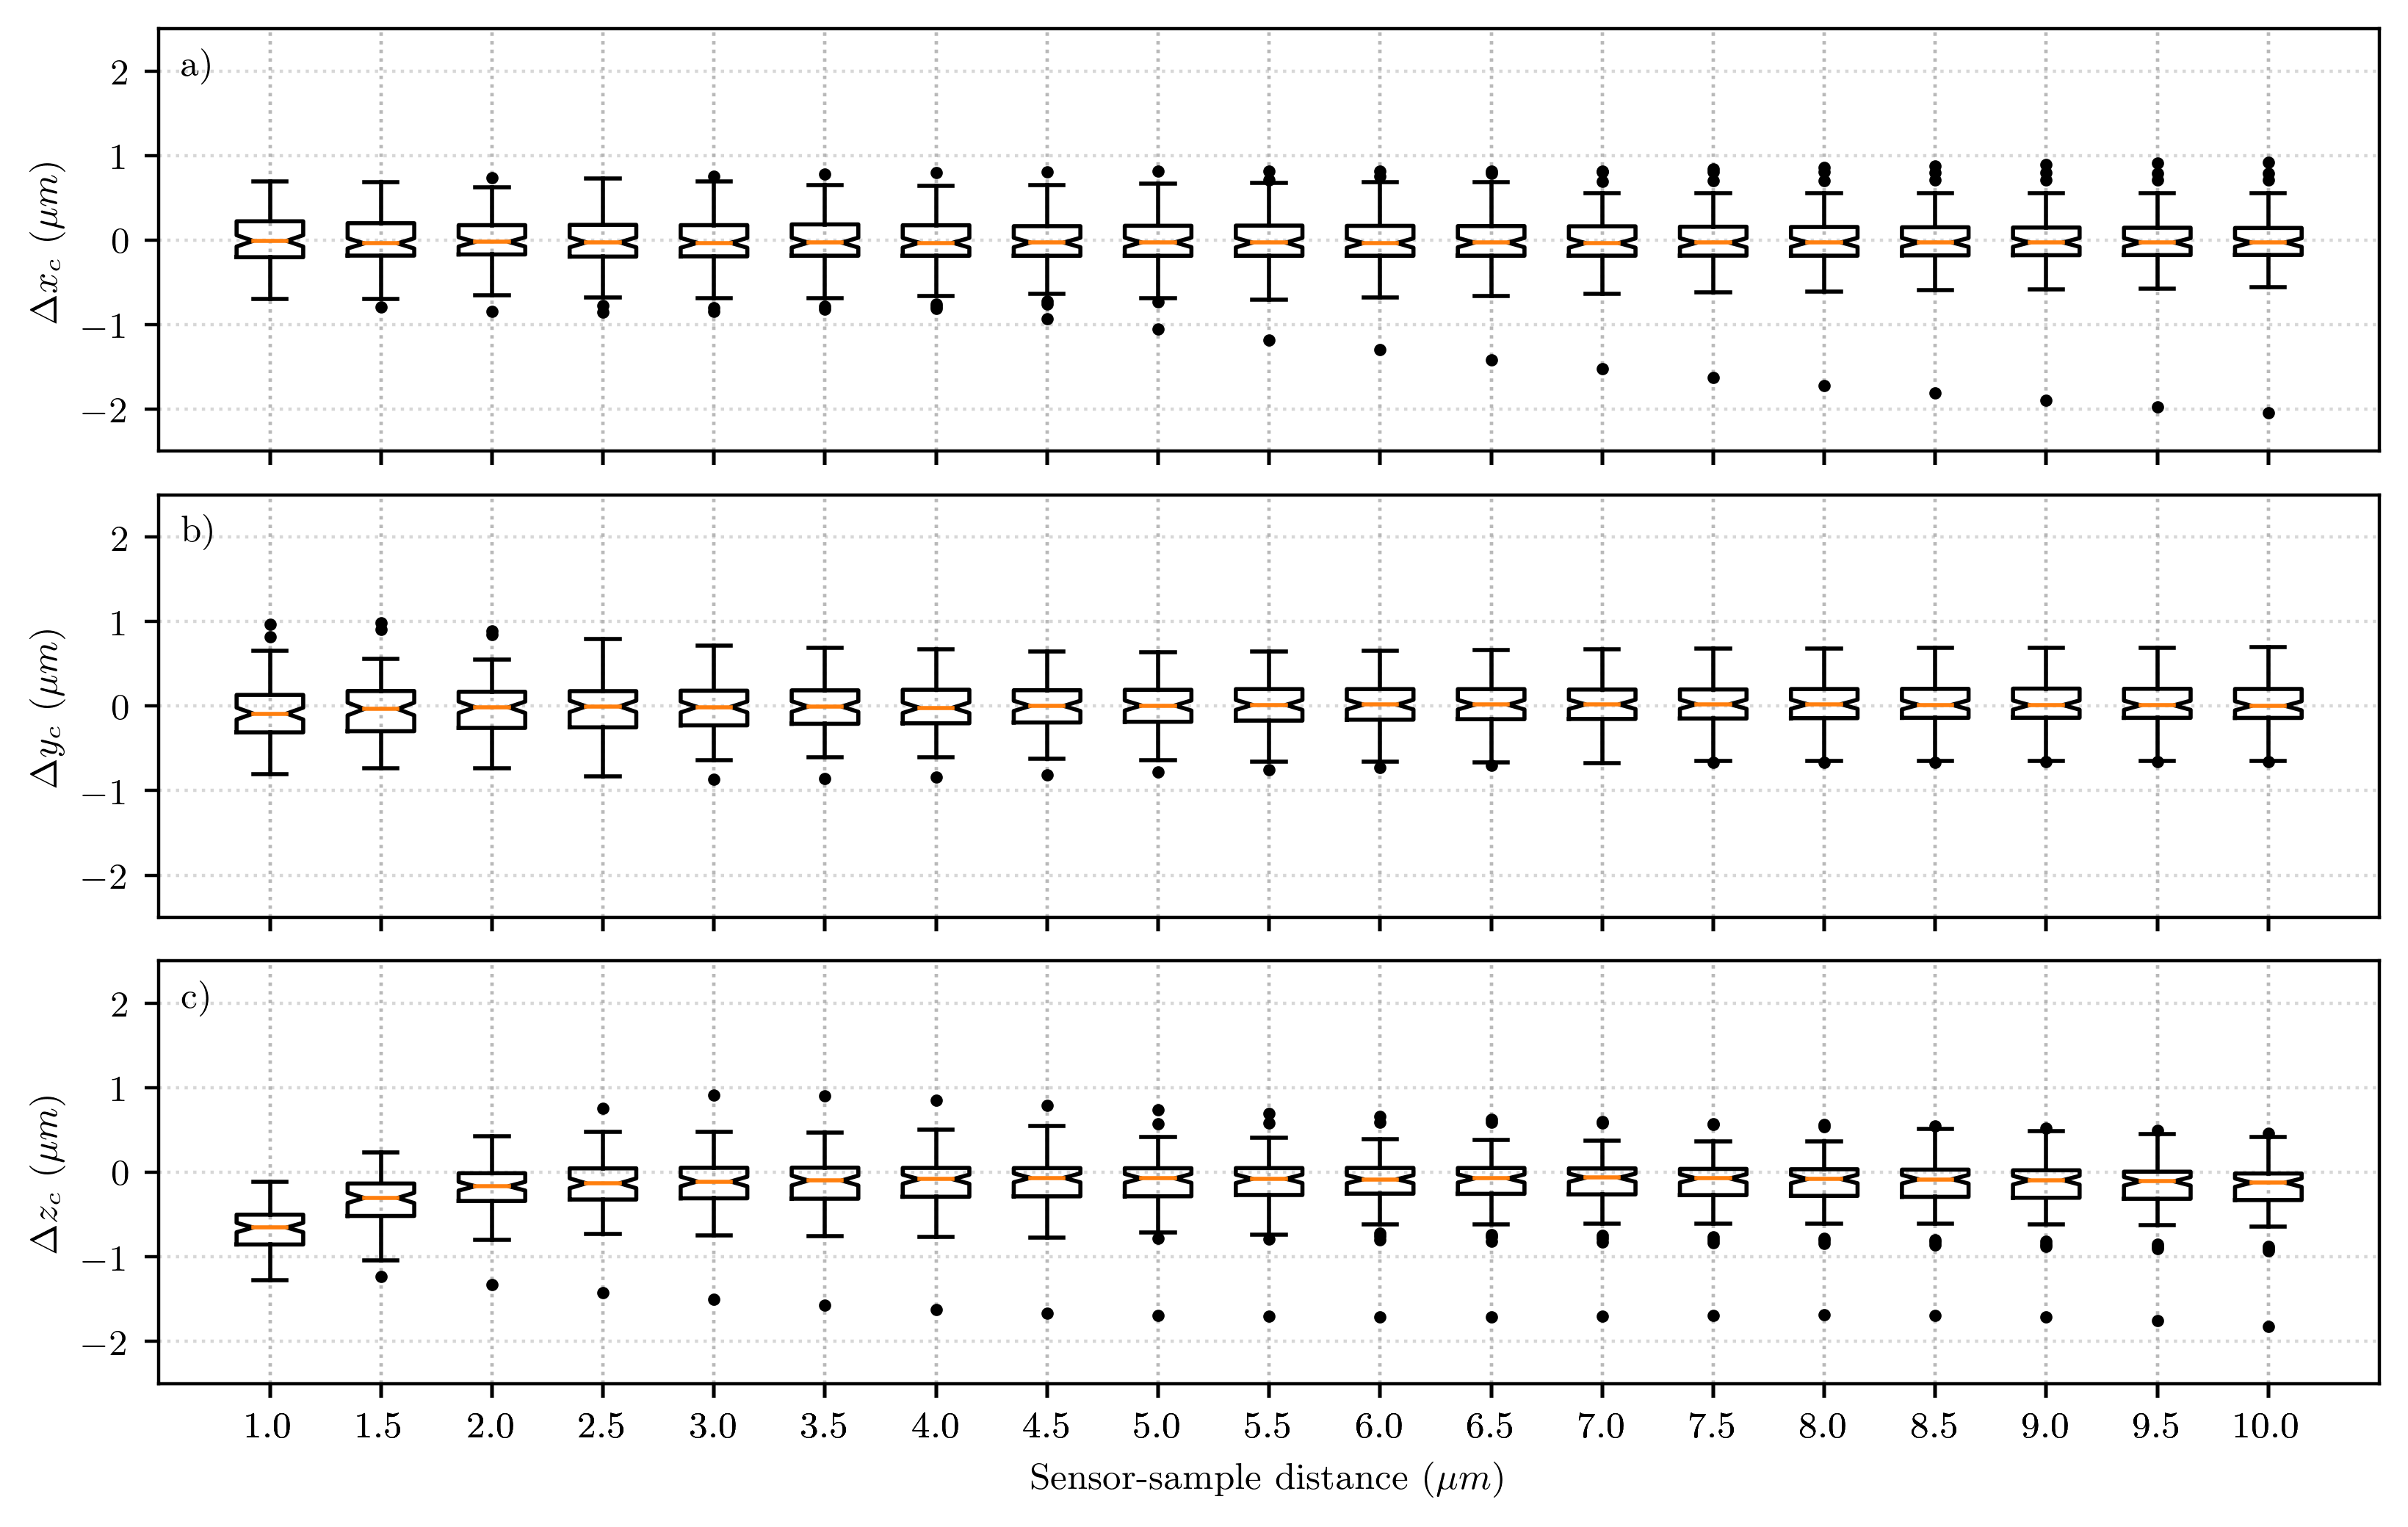
\includegraphics[width=1\linewidth]{micromag-euler-dipole/figures/non-dipolarity-synthetic-positioning.png}
  \caption{The simulation was randomly replicated (N=100) to test the effectiveness of the Euler deconvolution in estimating the position of the modeled particles. The difference between the true position (centroid) and the estimated position was calculated for each replicate and plotted as a boxplot. The boxplot shows the distribution of differences in the (a) $x_c$, (b) $y_c$, and (c) $z_c$. The black dots represent outliers in the distributions.}
  \label{non-dipolarity-synthetic-data-positioning}
\end{figure}

\begin{figure}[tb!]
  \centering
  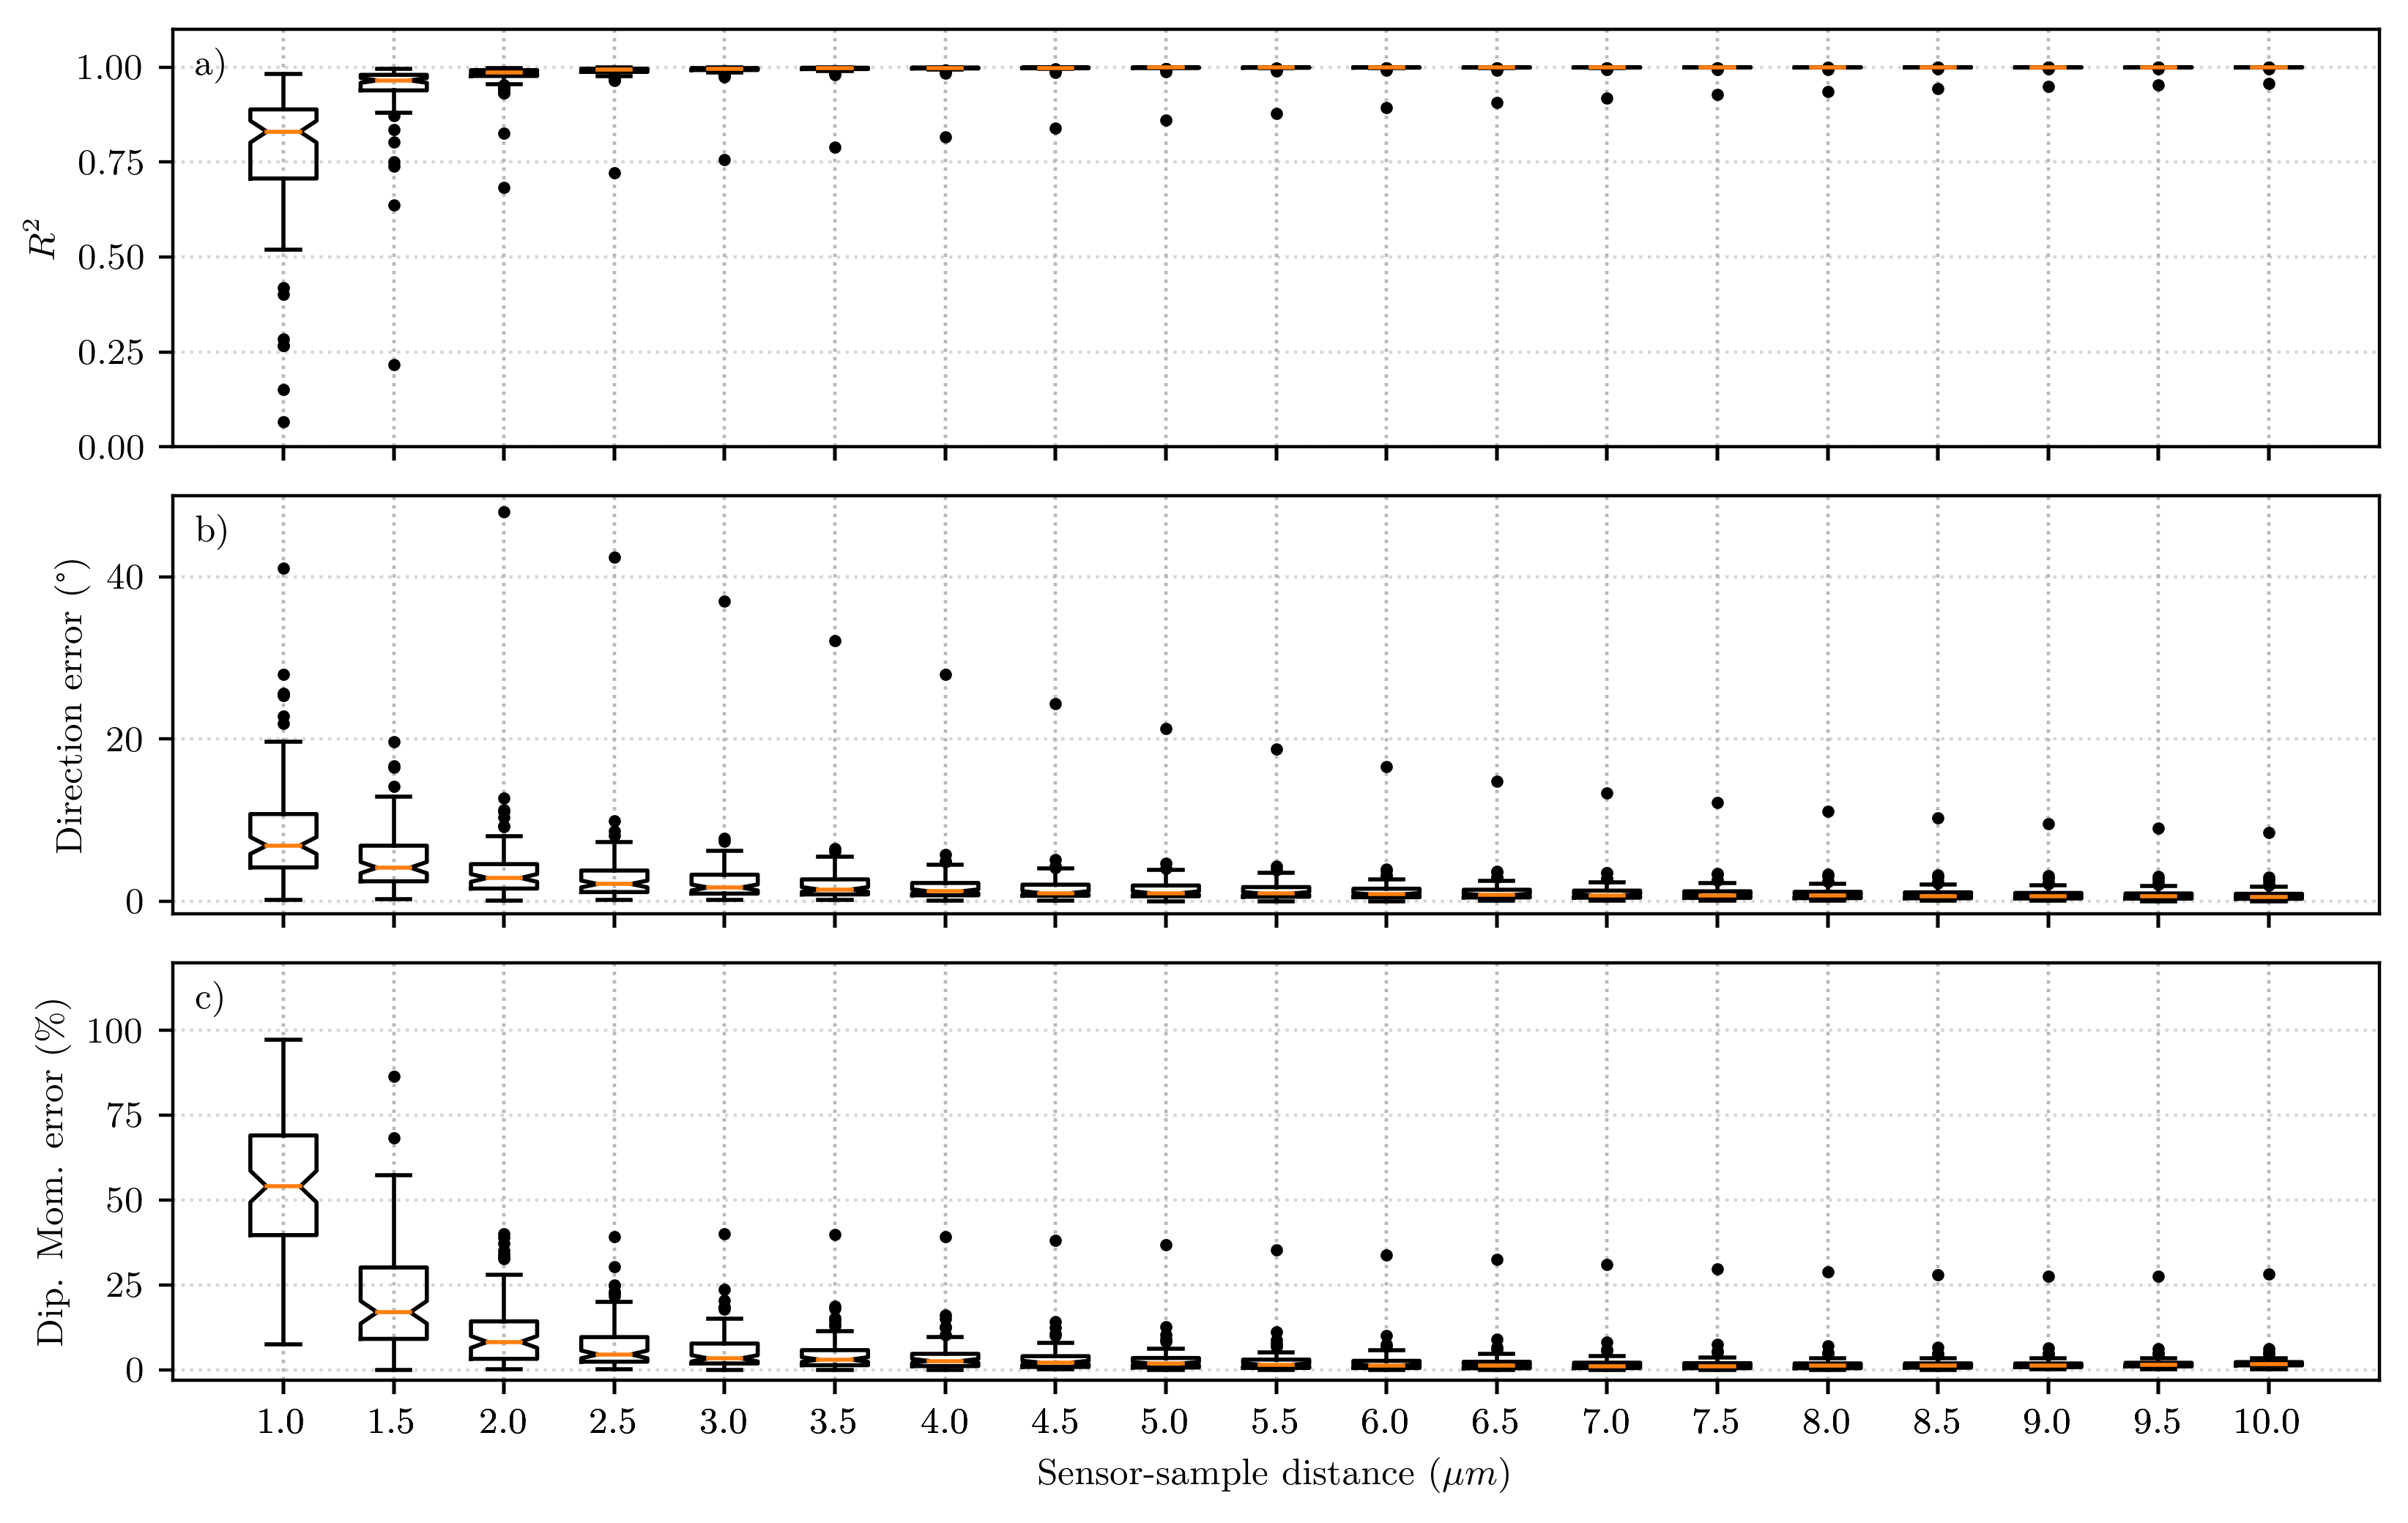
\includegraphics[width=1\linewidth]{micromag-euler-dipole/figures/non-dipolarity-synthetic-inversion.png}
  \caption{The simulation was randomly replicated (N=100) to assess the accuracy of the algorithm in recovering the magnetic direction and moment of the modeled particles. The goodness of fit was measured by the R-squared value (a), while the angular error (b) and intensity error (c) between the real and modeled magnetic vector were plotted in degrees and percentages ($|100 \left( m_{true} - m_{estimated}\right) ~/~ m_{true}|$), respectively. The black dots represent outliers in the distributions.
}
  \label{non-dipolarity-synthetic-data-inversion}
\end{figure}

\subsection{Applicability to more complex scenarios}

This test represents a more complex scenario by simulating typical grain distributions found in speleothem datasets.
The model is comprised of 103 sources randomly distributed in the imaged area of a synthetic thin section of $\qty{2000}{\um} \times \qty{2000}{\um}$.
The synthetic $b_z$ data were generated on a regular grid with $\qty{2}{\um}$ spacing and $\qty{5}{\um}$ sensor-sample distance.
We contaminated the data with high-frequency normally-distributed pseudo-random noise with zero mean and $\qty{50}{\nano\tesla}$ standard deviation, as well as with low-frequency noise in the form of additional deep sources beyond the modeling domain.

For greater fidelity to real samples, the magnetic sources are modeled as dipoles with different depths and magnetic moment intensities.
The depths vary randomly between 1 and $\qty{20}{\um}$, while the dipole moment intensities range randomly from $10^{-11}$ to $\qty{e-14}{\ampere\m\squared}$.
The NRM found in real ferromagnetic particles varies individually but averages out to the inducing field direction.
To simulate this behavior in our synthetic data, we sample the source dipole moment directions from two pseudo-random Gaussian distributions.
The first group of sources ($M = 70$) are sampled from a distribution  with mean of $D = \ang{0}$ and $I = \ang{0}$ and standard deviation of $\ang{10}$.
The second group of sources ($M = 30$) are sampled from a distribution with mean of $D = \ang{180}$ and $I = \ang{0}$, also with standard deviation of $\ang{10}$. We also manually added 3 sources with higher dipole moments ($5 \times 10^{-11}$) to further simulate the complexity observed in real data measurements. The noise-corrupted synthetic $b_z$ data are shown in Figure~\ref{complex-synthetic-data}a.

\begin{figure}[tb!]
  \centering
  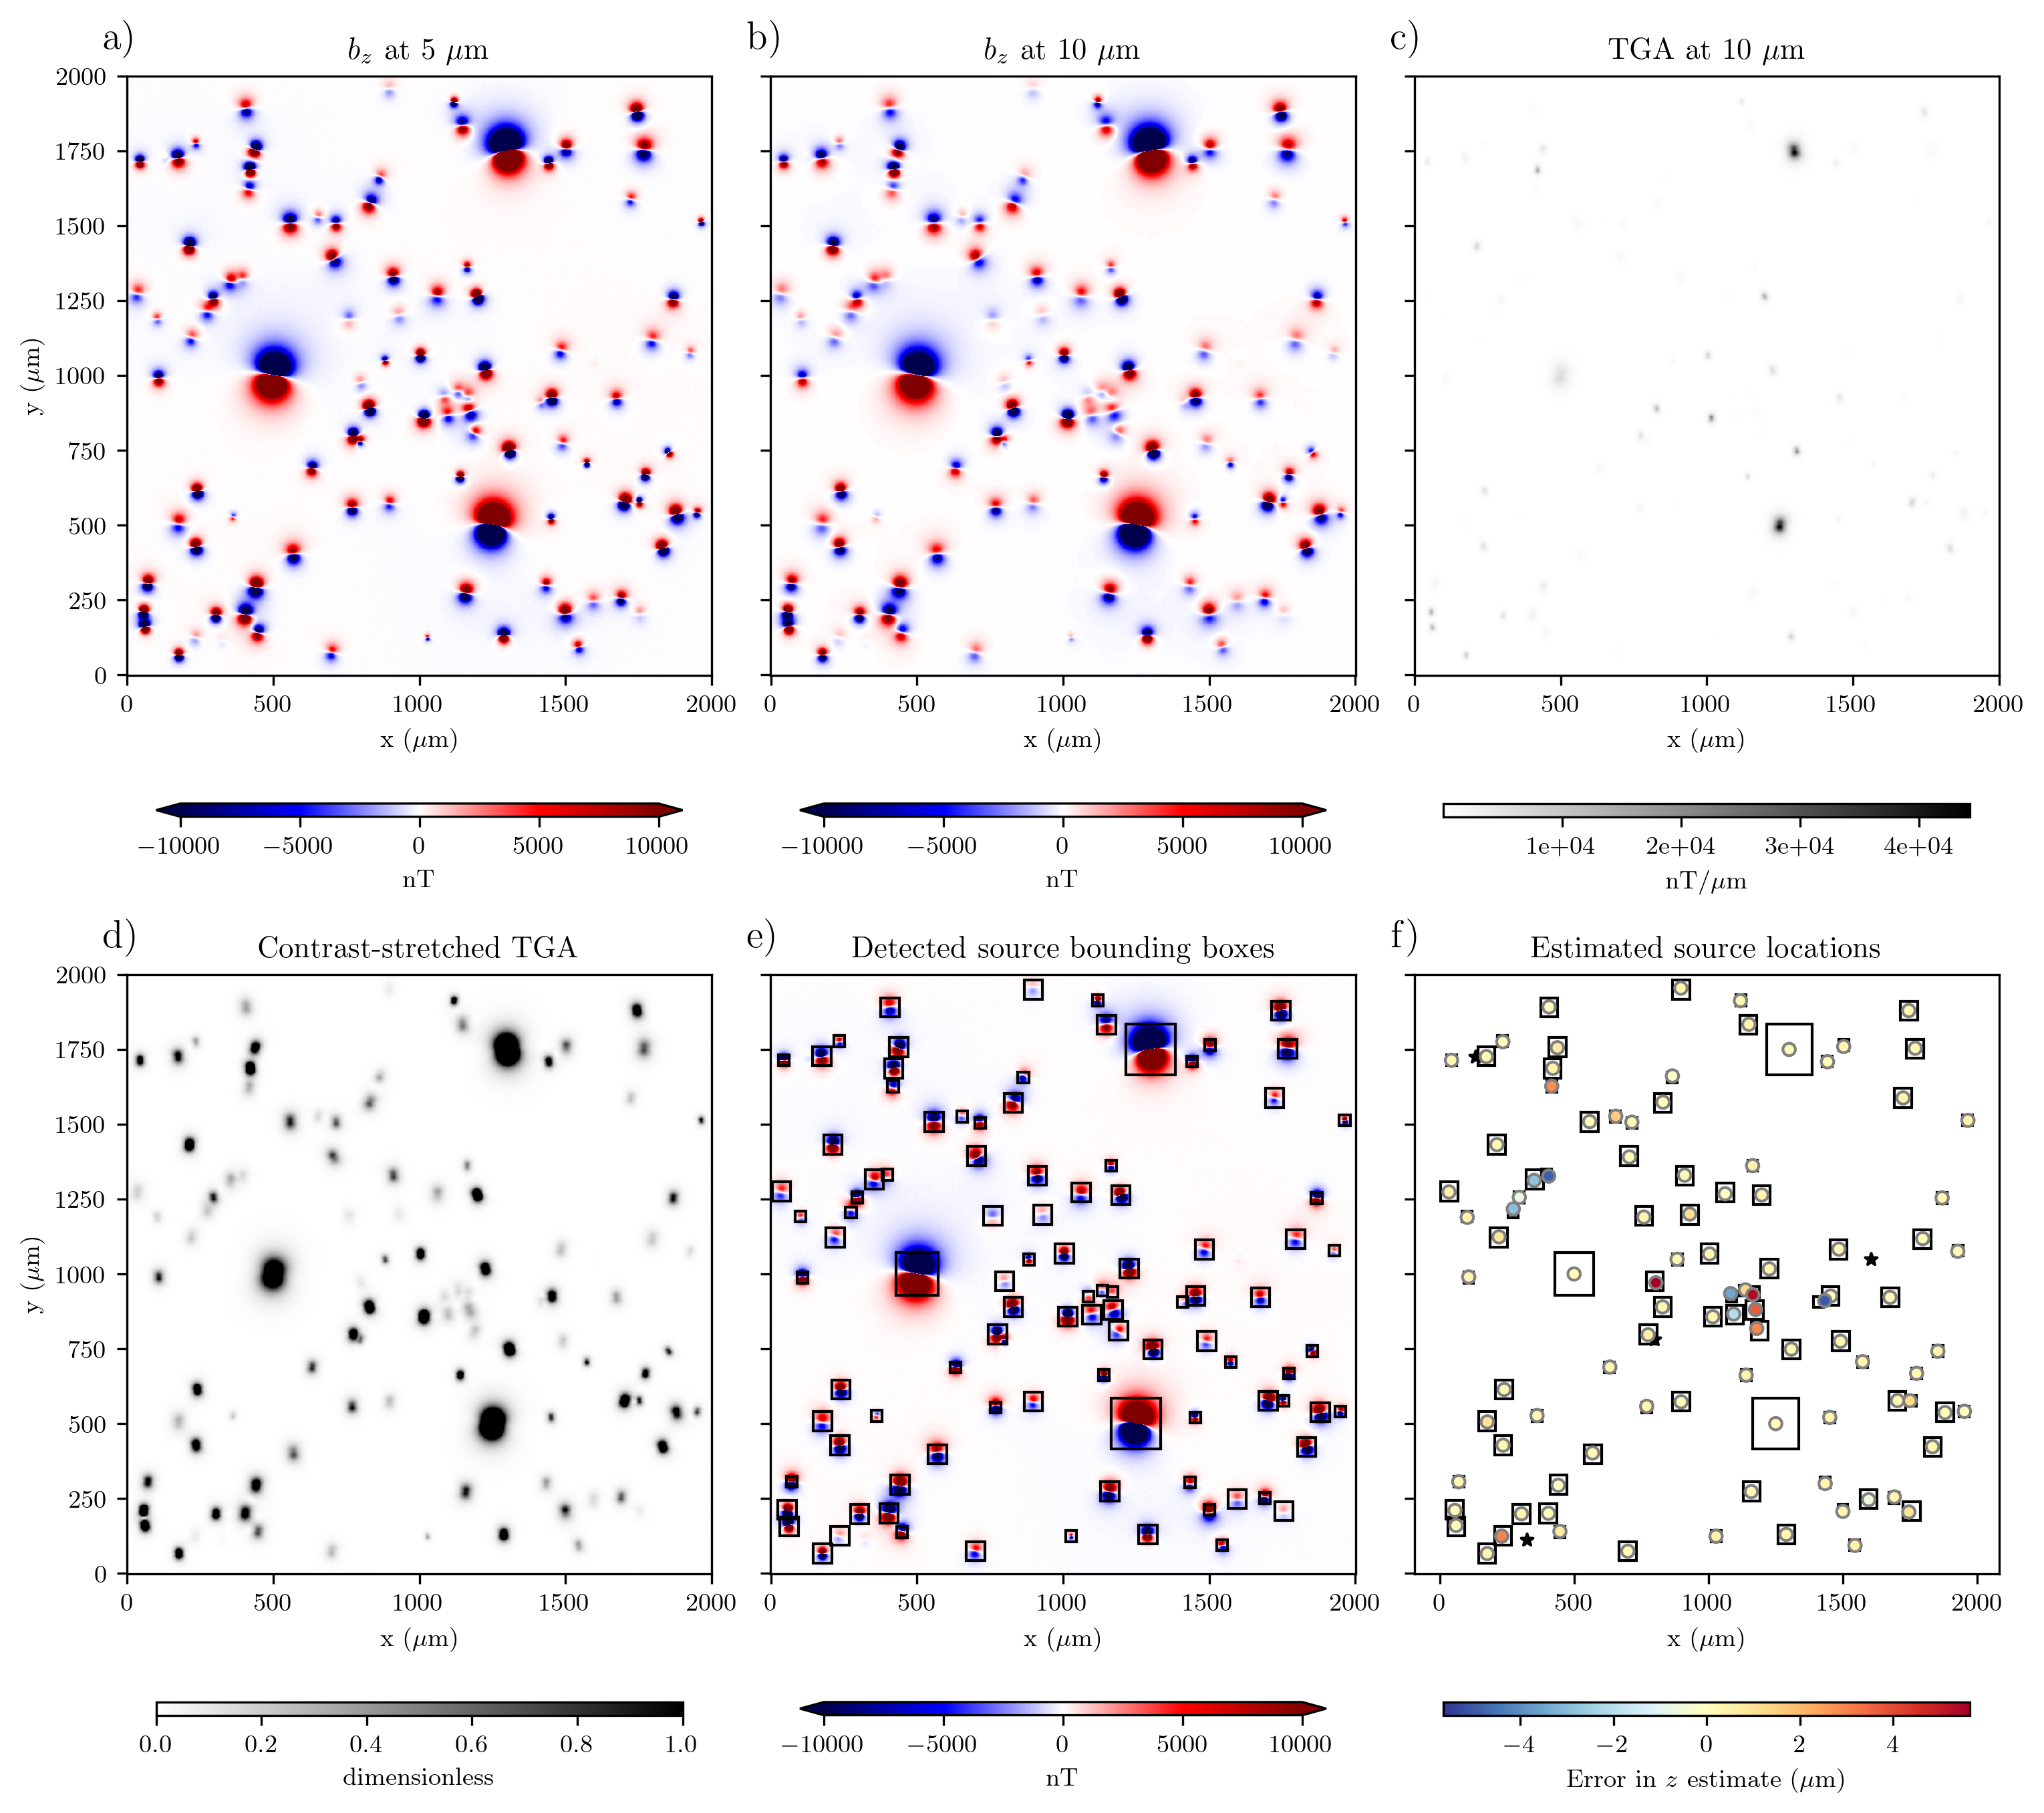
\includegraphics[width=1\linewidth]{micromag-euler-dipole/figures/complex-synthetic-data.png}
  \caption{
    Complex synthetic data and the various processing steps performed prior to the dipole moment inversion.
    a) The synthetic high and low-frequency noise-corrupted $b_z$ observations at
    $z = \qty{5}{\micro\meter}$ due to two clusters of stable directions simulated.
    b) Anomaly map after upward-continuation to $z = \qty{10}{\micro\meter}$ to attenuate short-wavelength noise.
    c) The total gradient amplitude (TGA) calculated from the
    upward-continued data, which is able to concentrate the signal on top
    of each dipolar source.
    d) The contrast-stretched TGA, highlighting the signal of all sources, especially the weaker ones.
    e) The detected source bounding boxes (black squares) that correctly
    encapsulate the signal of the sources.
    f) The estimated source locations (colored circles) from Euler
    Deconvolution of the upward-continued data inside each bounding box.
    The color represents the difference between the true and estimated
    $z$ coordinates.
  }
  \label{complex-synthetic-data}
\end{figure}

We then followed the same processing steps as for the simple synthetic: upward continuation (Figure~\ref{complex-synthetic-data}b),
TGA calculation (Figure~\ref{complex-synthetic-data}c), contrast stretching (Figure~\ref{complex-synthetic-data}d), blob detection (Figure~\ref{complex-synthetic-data}e), and Euler Deconvolution (Figure~\ref{complex-synthetic-data}e).
The Euler deconvolution and dipole moment inversion took approximately 1.5 seconds to compute, while
the source detection algorithm took approximately 8 seconds, on a laptop with an Intel(R) Core(TM) i7-2670QM CPU 2.20GHz with 16 GB of DDR3L 1333 MHz RAM.

A total of 99 sources out of the original 103 were successfully detected. Four sources remained unidentified (black stars in Figure~\ref{complex-synthetic-data}f) due to specific challenges, that arose from two primary factors:

\begin{enumerate}
    \item Three of these sources either overlapped with or were in close proximity to other neighboring sources, making it inherently difficult to distinguish and isolate them.
    \item The identification of one of these sources was impeded by its considerable depth, which led to substantial signal attenuation, further exacerbating the difficulties associated with source recognition.
\end{enumerate}

\begin{figure}[tb!]
\centering
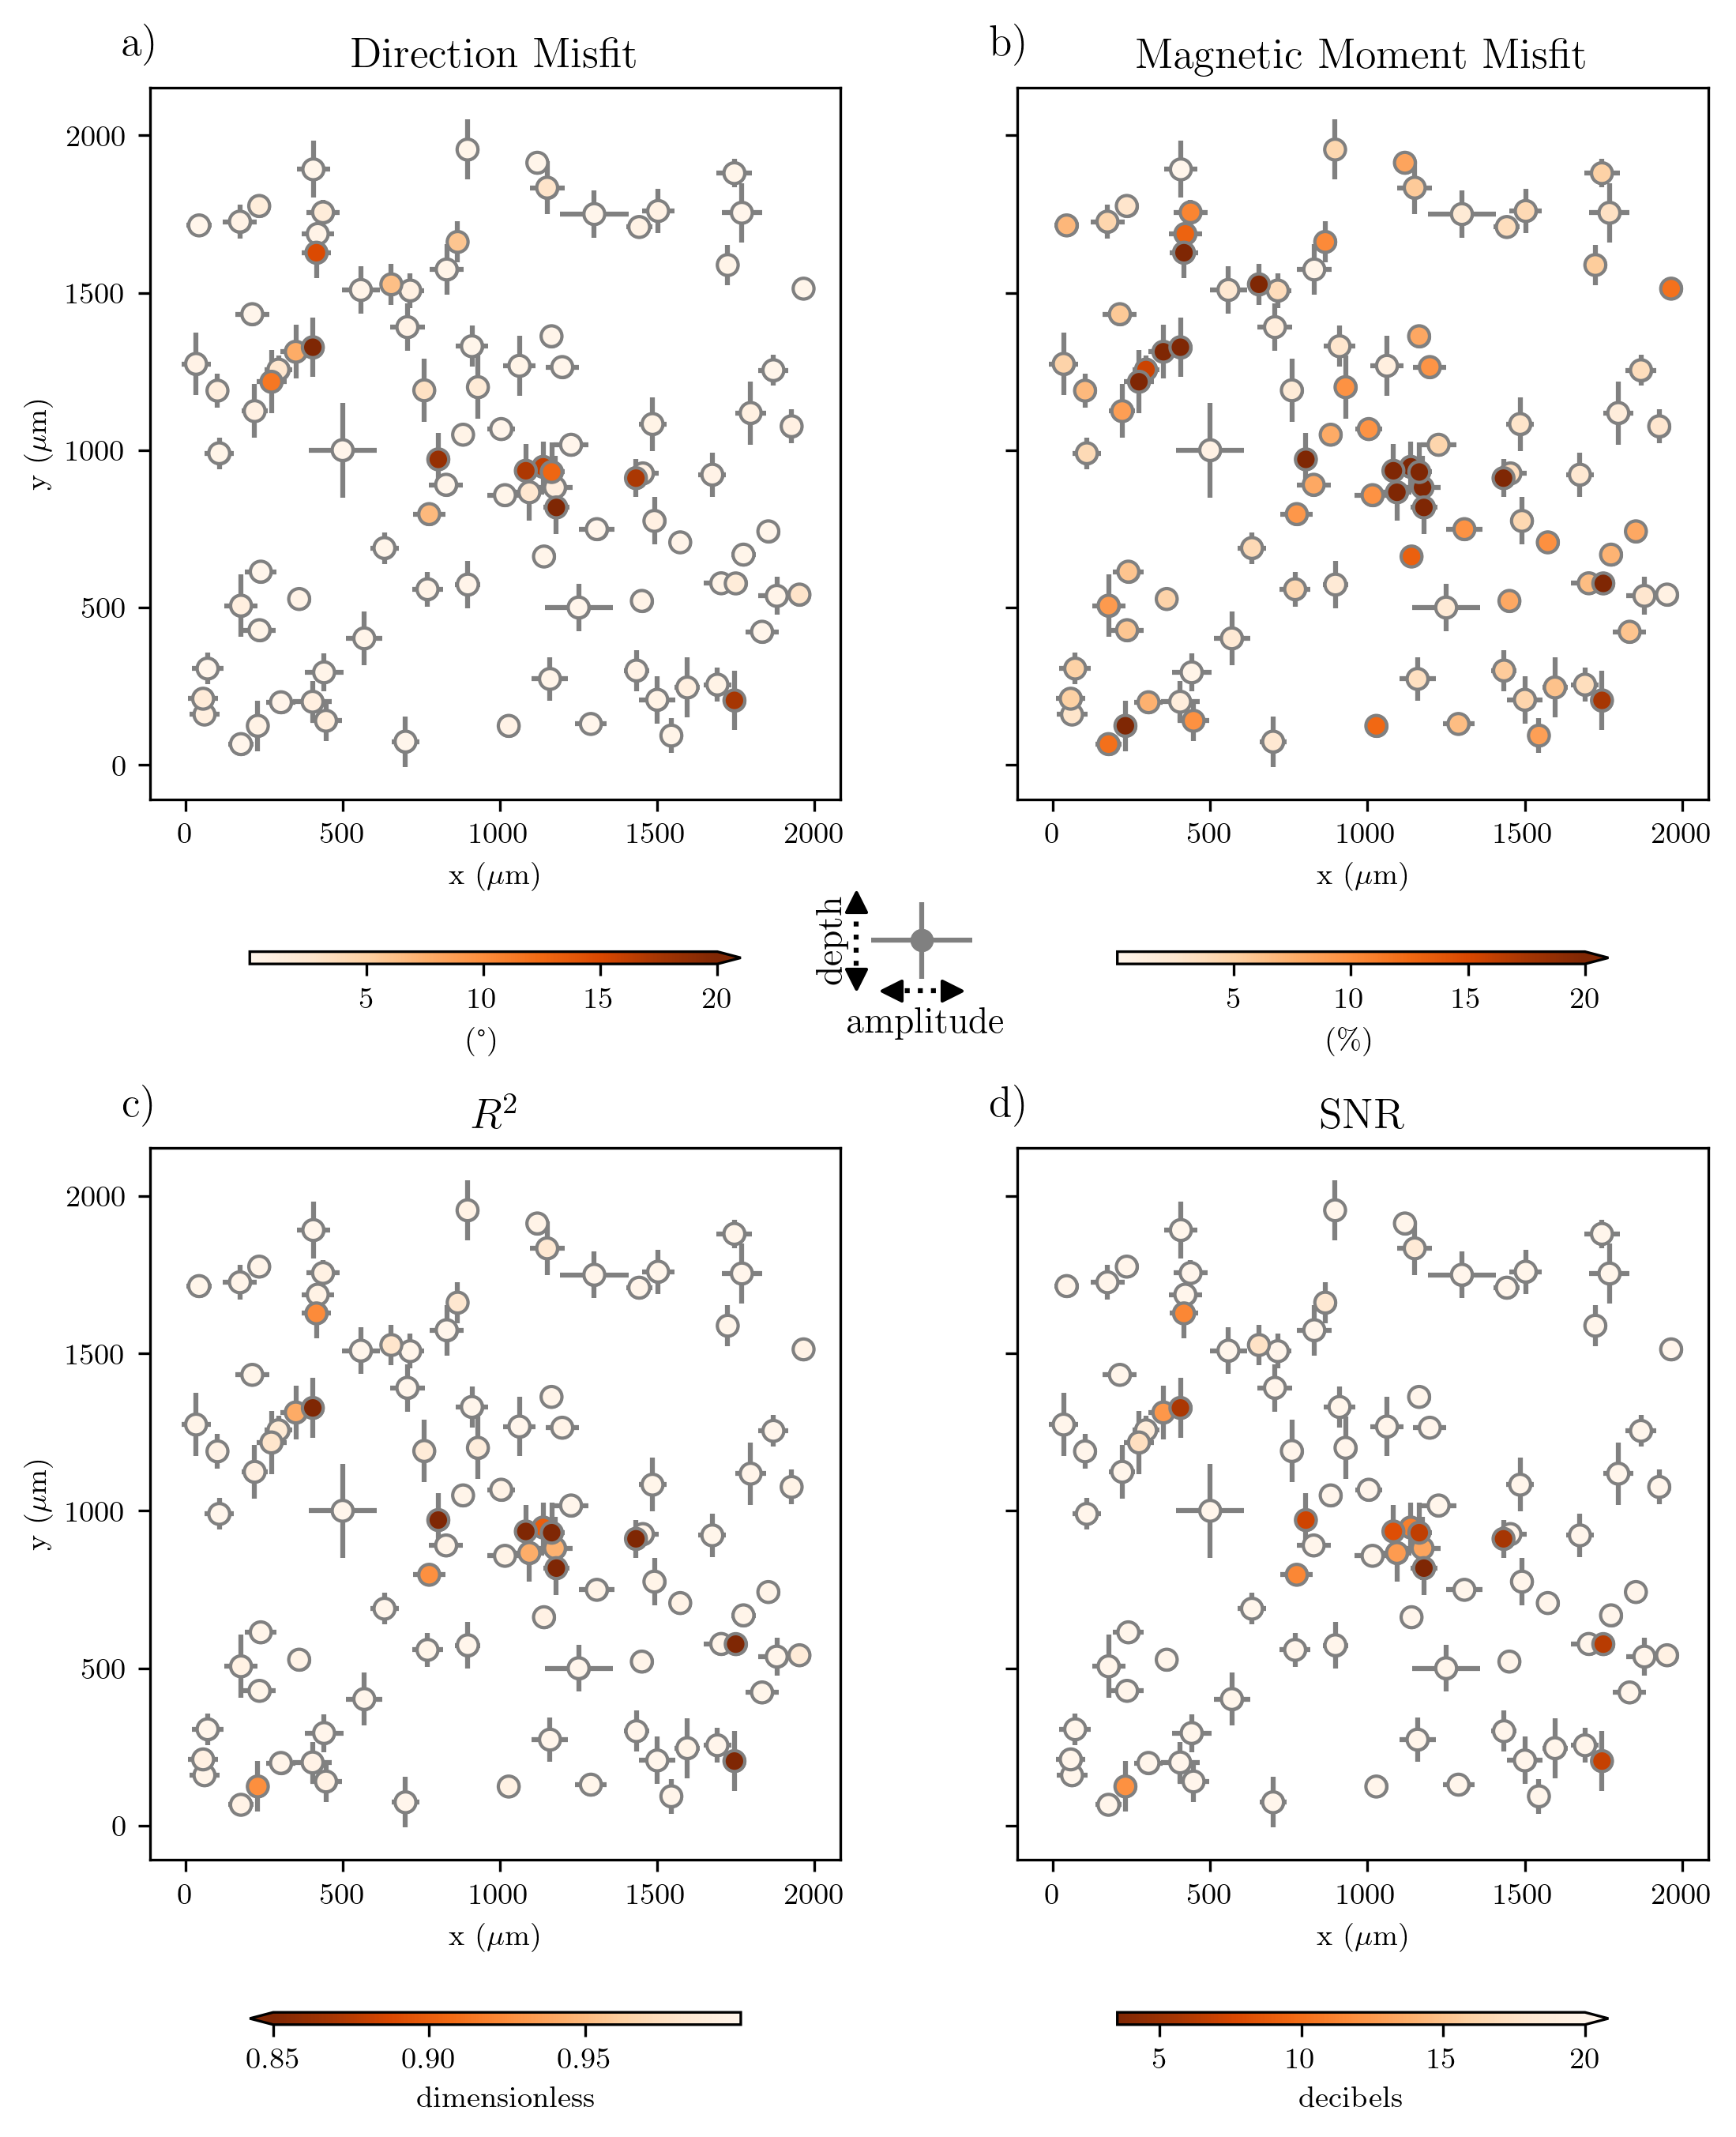
\includegraphics[width=0.75\linewidth]{micromag-euler-dipole/figures/complex-synthetic-comparison.png}
\caption{
The validation of the result obtained with the inversion was calculated for each individual particle based on the error between the real parameters modeled and their respective recovered values, being (a) the direction and (b) intensity of the magnetic moment, in addition to the $R^2$ score (c) obtained by comparing the forward model and the actual data. The depth and radius of the magnetic sources are also important factors that influence the final result, therefore, these data are given in the form of cross plots, with the vertical bar represented by the depth (1 - \qty{20}{\um}) and the horizontal bar by the dipole moment amplitude ($10^{-11}$ to $\qty{e-14}{\ampere\m\squared}$).
}
\label{complex-synthetic-comparison}
\end{figure}

The spatial resolution of the inversion results is one of the key advantages of magnetic microscopy over the classic techniques of paleomagnetism.
Therefore, we present the inversion results spatially so that we can evaluate any patterns in their distribution.
Figure~\ref{complex-synthetic-comparison} shows the spatial locations of the 99 sources that were identified and the differences between the estimated dipole moments and the true values.
The depth and dipole moment amplitude of each source are represented by horizontal and vertical bars, respectively.
These two variables are useful proxies for the strength and spatial extent of the signal of each source,
which can tell us about the limitations in strengths and sizes of the source signal that the technique is able to correctly invert.
Figure~\ref{complex-synthetic-comparison}a shows the absolute value of the angular difference between the true and the estimated dipole moment vectors.
Figure~\ref{complex-synthetic-comparison}b shows the percentage difference between the true and estimated dipole moment magnitudes ($|100 \left( m_{true} - m_{estimated}\right) ~/~ m_{true}|$).
Figure~\ref{complex-synthetic-comparison}c shows the $R^2$ coefficient (Equation~\ref{eq_r2}), which is equivalent to the non-dipolarity parameter of \citet{Fu2020} and represents how well the dipolar model is able to explain the observed data of each source.
Figure~\ref{complex-synthetic-comparison}d shows the SNR (Equation~\ref{eq_snr}), which expresses the power of the observed data over that of the inversion residuals.
High SNR values correspond to small inversion residuals which indicate that a dipolar model was able to explain the observed data.
Consequently, the variation of SNR values is similar to that of the $R^2$ coefficient.
Figure~\ref{complex-synthetic-comparison} shows that large errors in the estimated dipole moment direction are associated with low values of $R^2$ and SNR.
Conversely, the correlation between errors in dipole moment magnitude and $R^2$ and SNR is less pronounced, with some poor magnitude estimates being associated with $R^2$ and SNR indicating a reasonable fit by a dipolar model.
It is also noticeable that the majority of cases where the direction misfit is given by deep and low-amplitude sources that are close to shallower or higher-amplitude sources.
These results indicated that $R^2$ and SNR can be used as selection criteria to discard sources with likely high errors in the estimated dipole moment.

\begin{figure}[tb!]
\centering
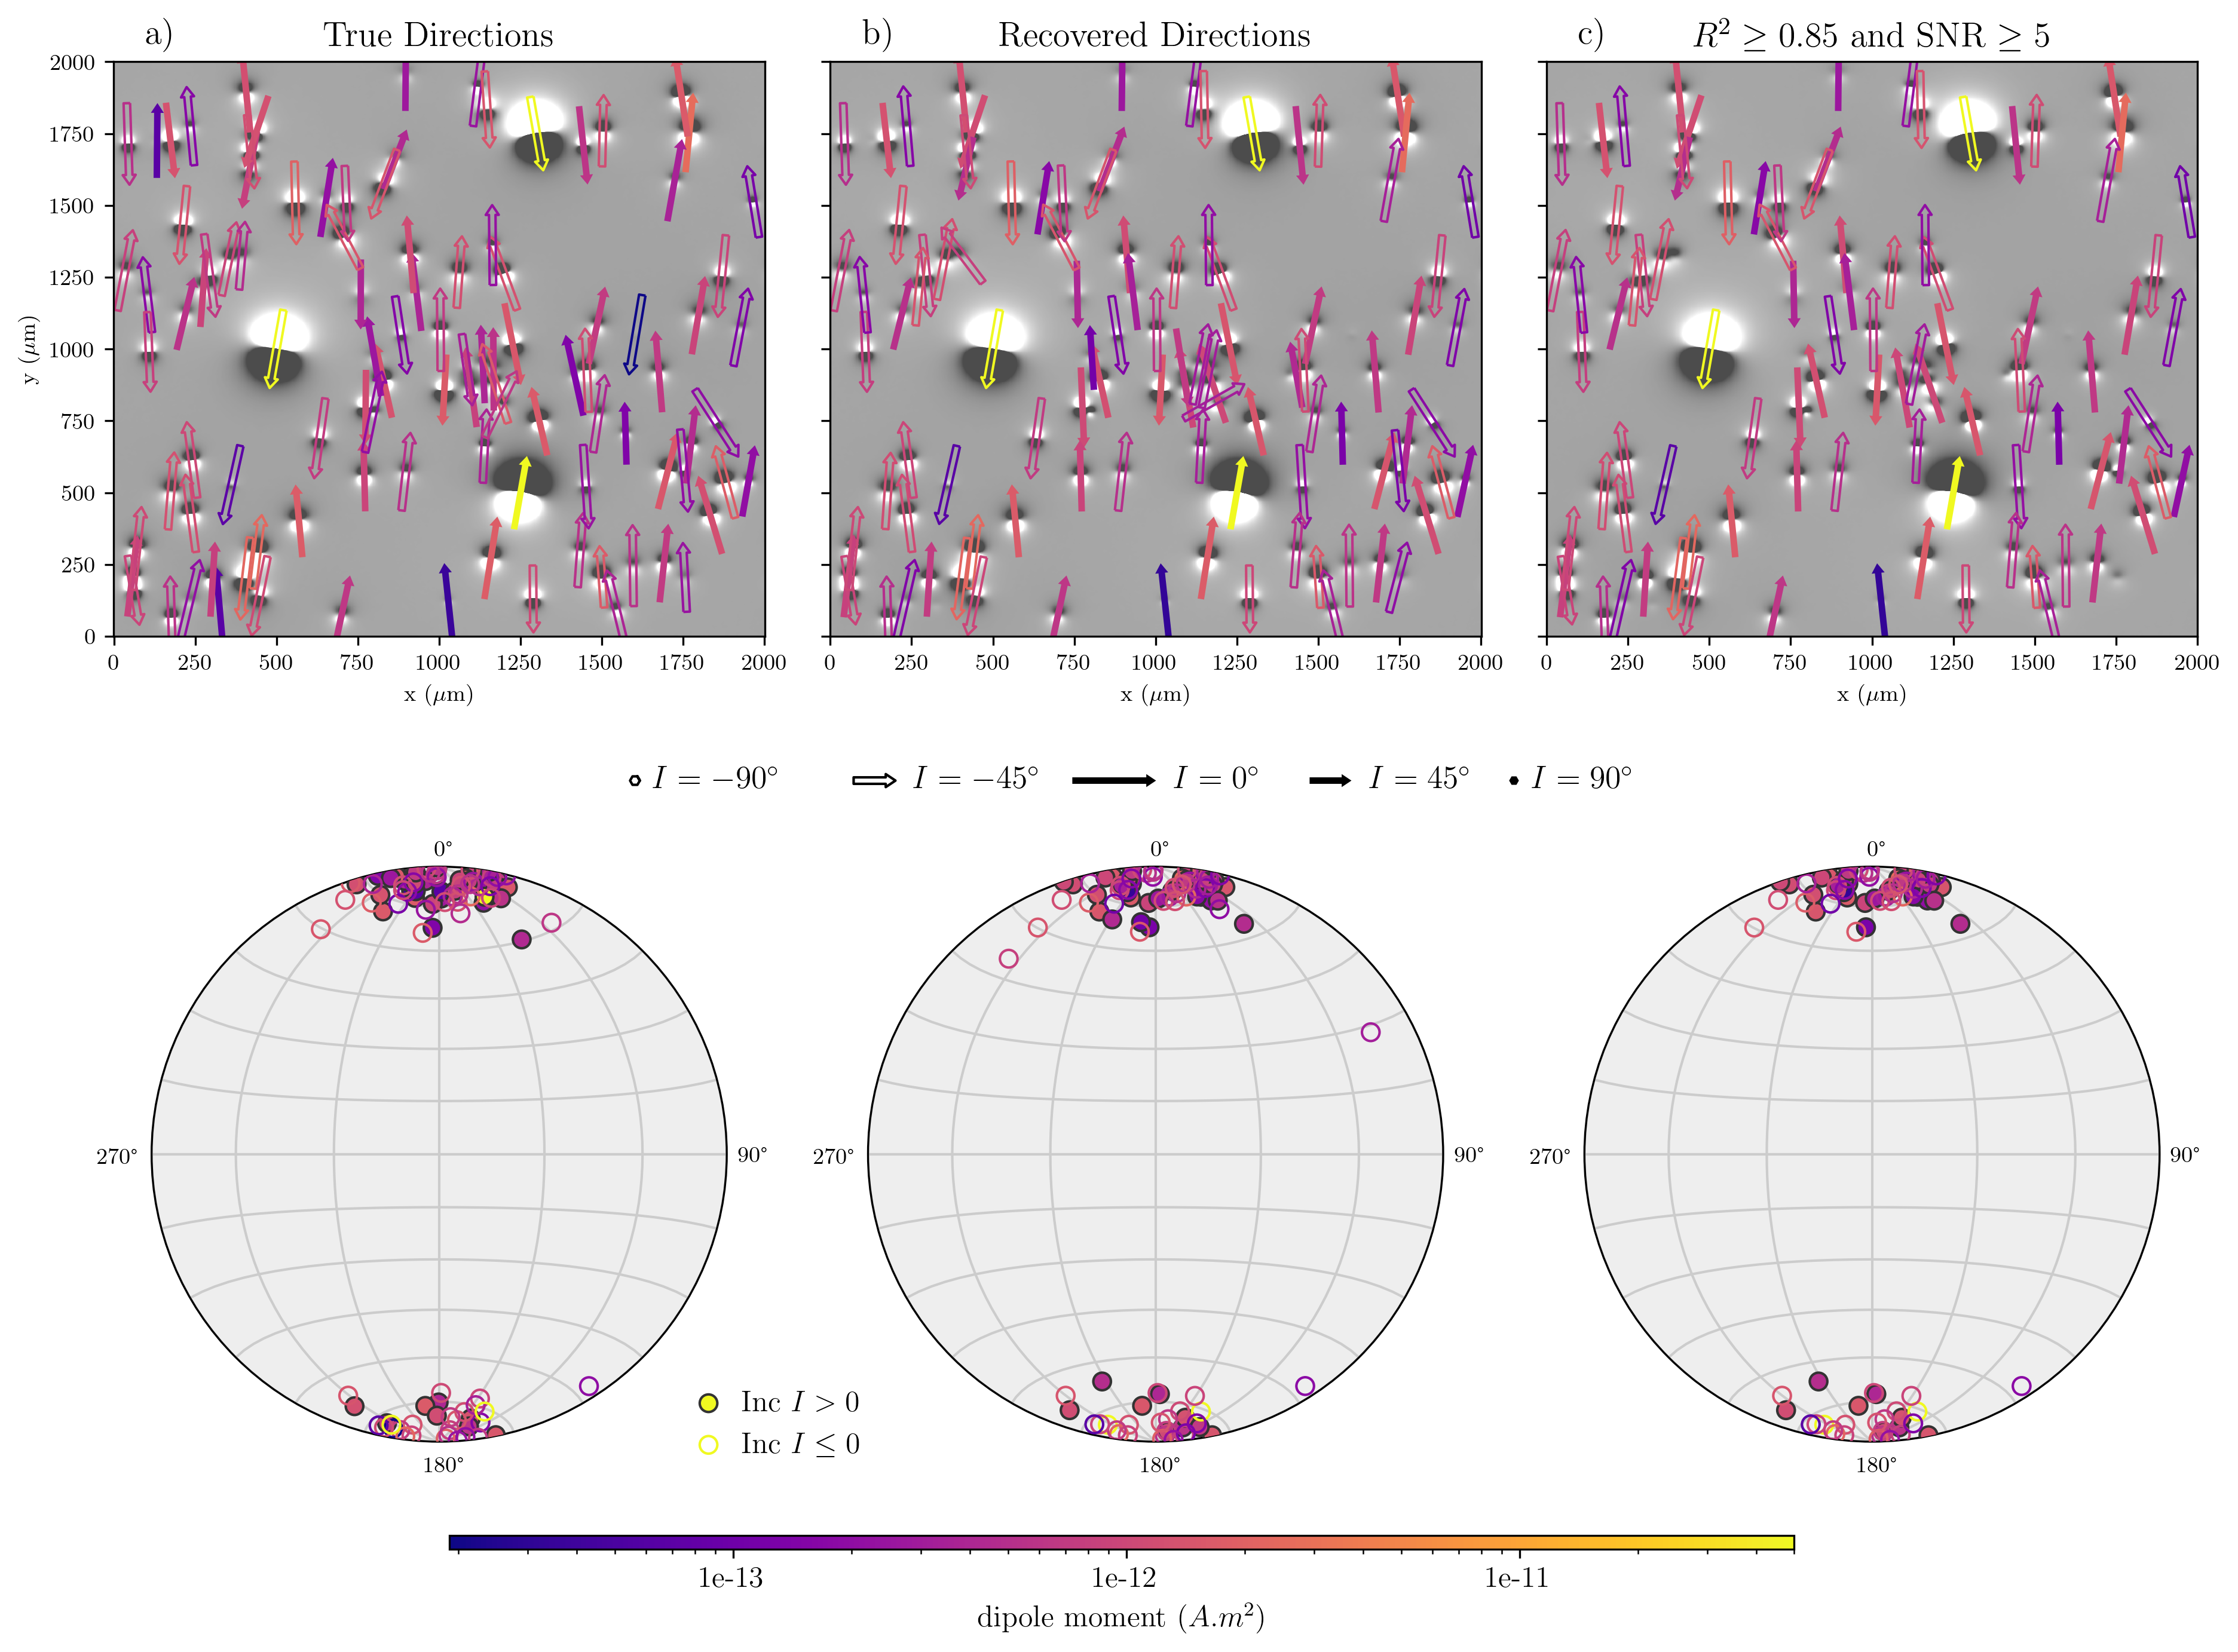
\includegraphics[width=1\linewidth]{micromag-euler-dipole/figures/complex-synthetic-stereograms.png}
\caption{ Comparison of true and estimated dipole magnetic moments and directions for the complex synthetic sample.
a) Simulation of a thin section of rock with 103 particles uniformly magnetized (dipolar sources) by two different induced fields. The average directions of the induced fields are $D=\ang{0}$ / $I=\ang{0}$ and $D=\ang{180}$ / $I=\ang{0}$, yielding two stable directions. b) All estimated vector directions of the identified sources ($M=99$). c) The Filtering criteria used to select the magnetic directions of the sources with the best fitting ($M=96$), determined by the coefficient of determination ($R^2 \geq 0.85$) and signal-to-noise ratio ($\text{SNR} \geq 5$).
}
\label{complex-synthetic-stereograms}
\end{figure}

Figure~\ref{complex-synthetic-stereograms} shows stereograms with the directions generated by the modeled (Figure~\ref{complex-synthetic-stereograms}a) and the estimated vectors (Figure~\ref{complex-synthetic-stereograms}b) for each source. The distribution of the estimated directions is coincident with the true directions aside from a few sources, the same ones with the higher values of direction misfit (Figure~\ref{complex-synthetic-comparison}a) which is probably associated with the mutual interference of sources close to each other or within the same window. When filtered to include only data with $R^2 \geq 0.85$ and $\text{SNR} \geq 5$ the obtained direction distribution is closer to the true distribution (Figure~\ref{complex-synthetic-stereograms}c).

\subsection{Applicability to different grain concentration scenarios}

In order to assess the algorithm's ability to work with samples featuring higher concentrations of particles, we conducted a test of our algorithm on multiple synthetic datasets with increasing concentrations of randomly distributed magnetic grains in a volume of $2000 \times 2000 \times \qty{20}{\um}$. For each concentration, we generated 15 different random grain distributions. Figure~\ref{grain-concentration}a depicts the percentage of particles detected by the algorithm, with the median of the distribution represented by the red line. The same figure also presents the percentage of particles whose inversion results meet the filtering criteria of $R^2 \geq 0.85$ and $\text{SNR} \geq 5$, with the median represented by the blue line. As the number of particles increases, there is a consistent decrease in the percentage of sources detected. This is expected because of the spatial constraints of the algorithm, which require magnetic sources to be spatially separated for the detection algorithm to identify them. As shown in Figure~\ref{grain-concentration}b, by calculating the angular misfit between the vector sum direction of the model and the vector sum direction of the detected windows, it is observed that, for the unfiltered windows (red line), the angular misfits tend to increase with the concentration of magnetic grains. Nonetheless, this angular misfit tends to approach zero when the filtering criteria are applied, regardless of the particle concentration.

This observation highlights the algorithm's ability to effectively filter out spurious sources and improve the reliability of the dipole moment estimation, particularly in scenarios with higher particle concentrations. These findings underscore the algorithm's robustness in handling varying sample conditions and its capacity to adapt to different levels of particle density. However, the same may not hold true for particle populations with many different dipole moment directions.

In addition to the test above, another synthetic data test was implemented using a gradual separation (between 0 and \qty{50}{\um}) of two dipolar sources. We also repeated the calculations for gradually increasing (between 0 and \qty{25}{\um}) the distance between the sources and the sensor. We then tracked when the source detection algorithm was able to find the two separate sources and when it found a single source. Figure~\ref{detection-map} illustrates the algorithm's performance concerning the separation of magnetic sources and varying sensor distances. In areas where the algorithm successfully discerns two distinct magnetic sources, the grid is shaded in blue. Conversely, the region shaded in red denotes instances where the algorithm detected only a single source with a data window encompassing the signal of both sources. In the case of shallow sources, the minimal distance necessary for the effective detection of both signals is approximately \qty{14}{\um}. This minimal distance exhibits a consistent increase with the sensor height, reaching up to approximately \qty{20}{\um} for the maximum modeled sensor distance.

\begin{figure}[tb!]
  \centering
  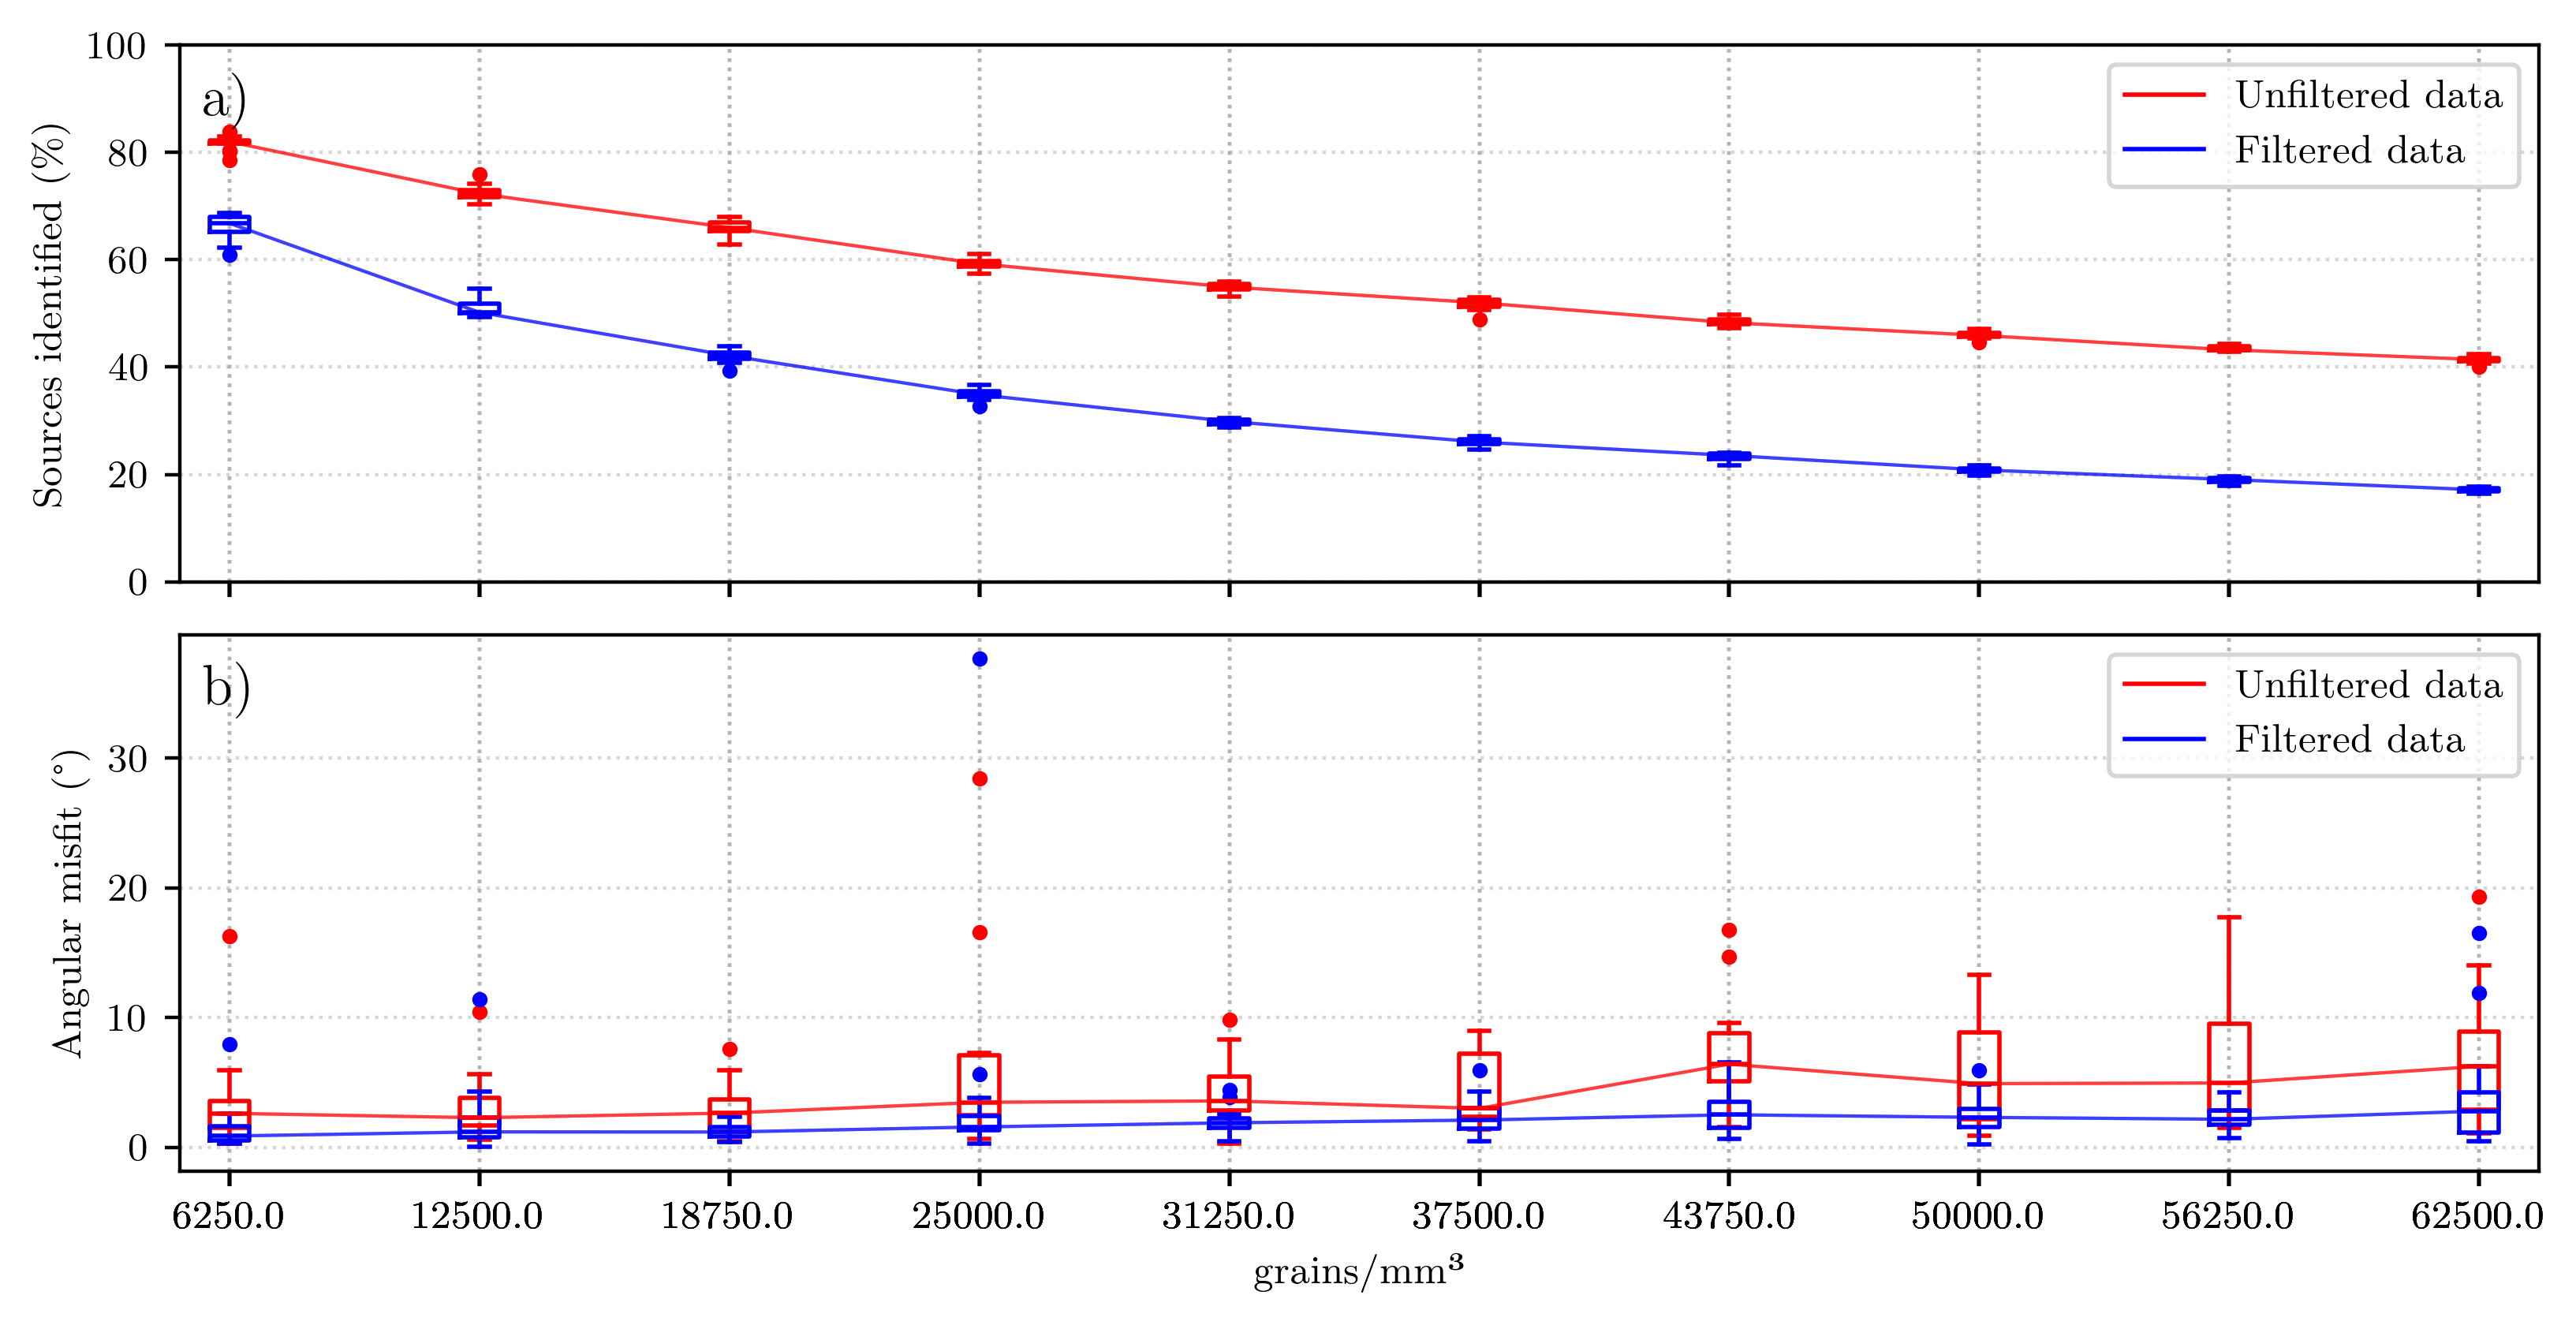
\includegraphics[width=1\linewidth]{micromag-euler-dipole/figures/grain_concentration.png}
  \caption{
  Different grain simulations were randomly replicated (N=15) to assess the effectiveness of the algorithm to detect the magnetic sources. a) The efficacy of the detection was measured by the percentage of sources identified ($100 \left( N_{detected} ~/~ N_{true} \right)$) and showed as box-plots for both unfiltered detection (median represented as the red line) and filtered detection ($R^2 \geq 0.85$ and $SNR \geq 5$, blue line). b) The same representation is displayed for the angular misfit between the true vector sum and both results for the filtered and unfiltered sum of vectors detected. The blue/red dots represent outliers in the distributions.
  }
  \label{grain-concentration}
\end{figure}

\begin{figure}[tb!]
\centering
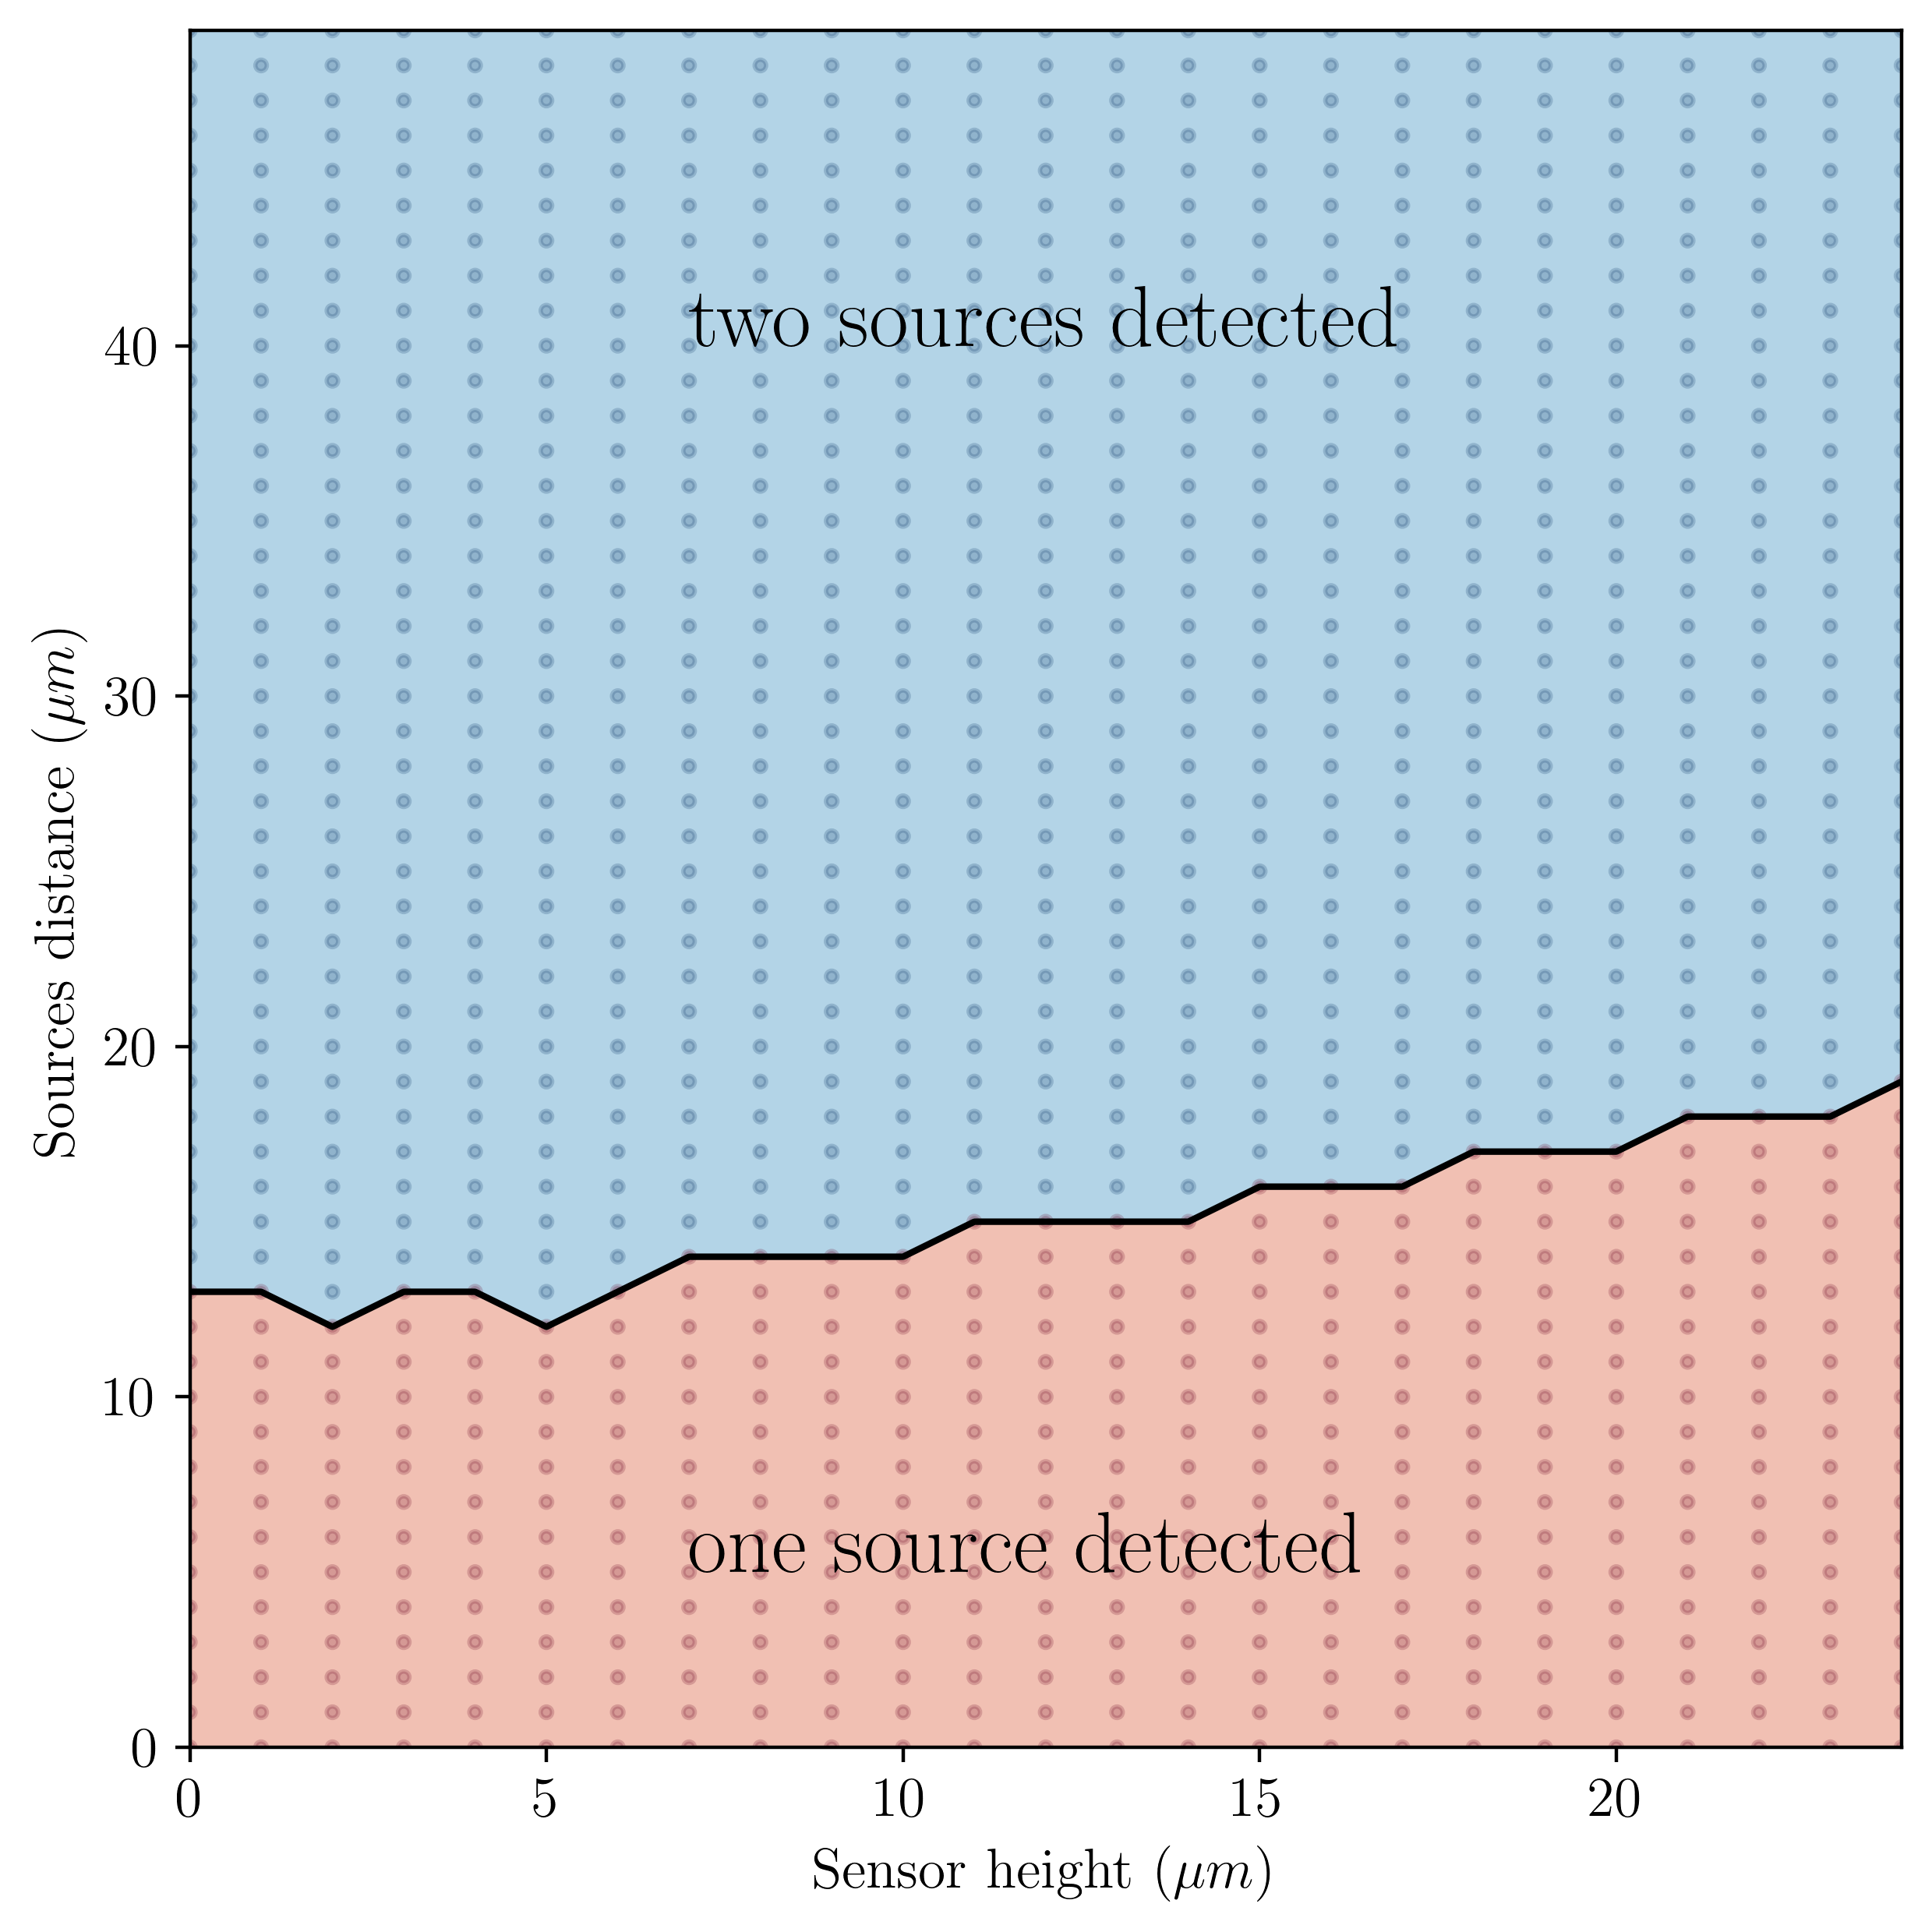
\includegraphics[width=0.5\linewidth]{micromag-euler-dipole/figures/detection-map.png}
\caption{
Simulation to assess the algorithm's ability to discern between two sources, with different horizontal separations and varying sensor-sample heights. The blue-shaded region signifies the successful detection of two distinct sources, while a red-shaded region indicates the detection of a single source due to closely spaced sources. The black line represents the boundary between these two regions.
}
\label{detection-map}
\end{figure}

%%%%%%%%%%%%%%%%%%%%%%%%%%%%%%%%%%%%%%%%%%%%%%%%%%%%%%%%%%%%%%%%%%%%%%%%%%%%%%%
\section{Application to real data}

To test whether the proposed method would be able to determine the
magnetization directions and the magnetic moment of particles in natural
samples, we selected a previously studied carbonate stalagmite sample from the
Wintimdouine cave in the Agadir region (Morocco) \citep{Ait2019Hydro}. This
speleothem contains both magnetite and hematite as the main carriers of
magnetic remanence, as attested by thermomagnetic curves with temperature
decays at {\textasciitilde}580 °C and {\textasciitilde}680 °C, and bimodal
curves of isothermal remanent magnetization (IRM) acquisition \citep{carmo2019speleothem}.

In order to provide two distinct directions associated with the different
magnetic mineral types in this sample, we applied two IRM pulse fields of 2.7 T
and 0.3 T, respectively toward the +Y and -Y directions. In this way, the high
coercivity grains (hematite) would point towards +Y and the low coercivity ones
(magnetite) would align in the -Y direction.

\begin{figure}[ph!]
\centering
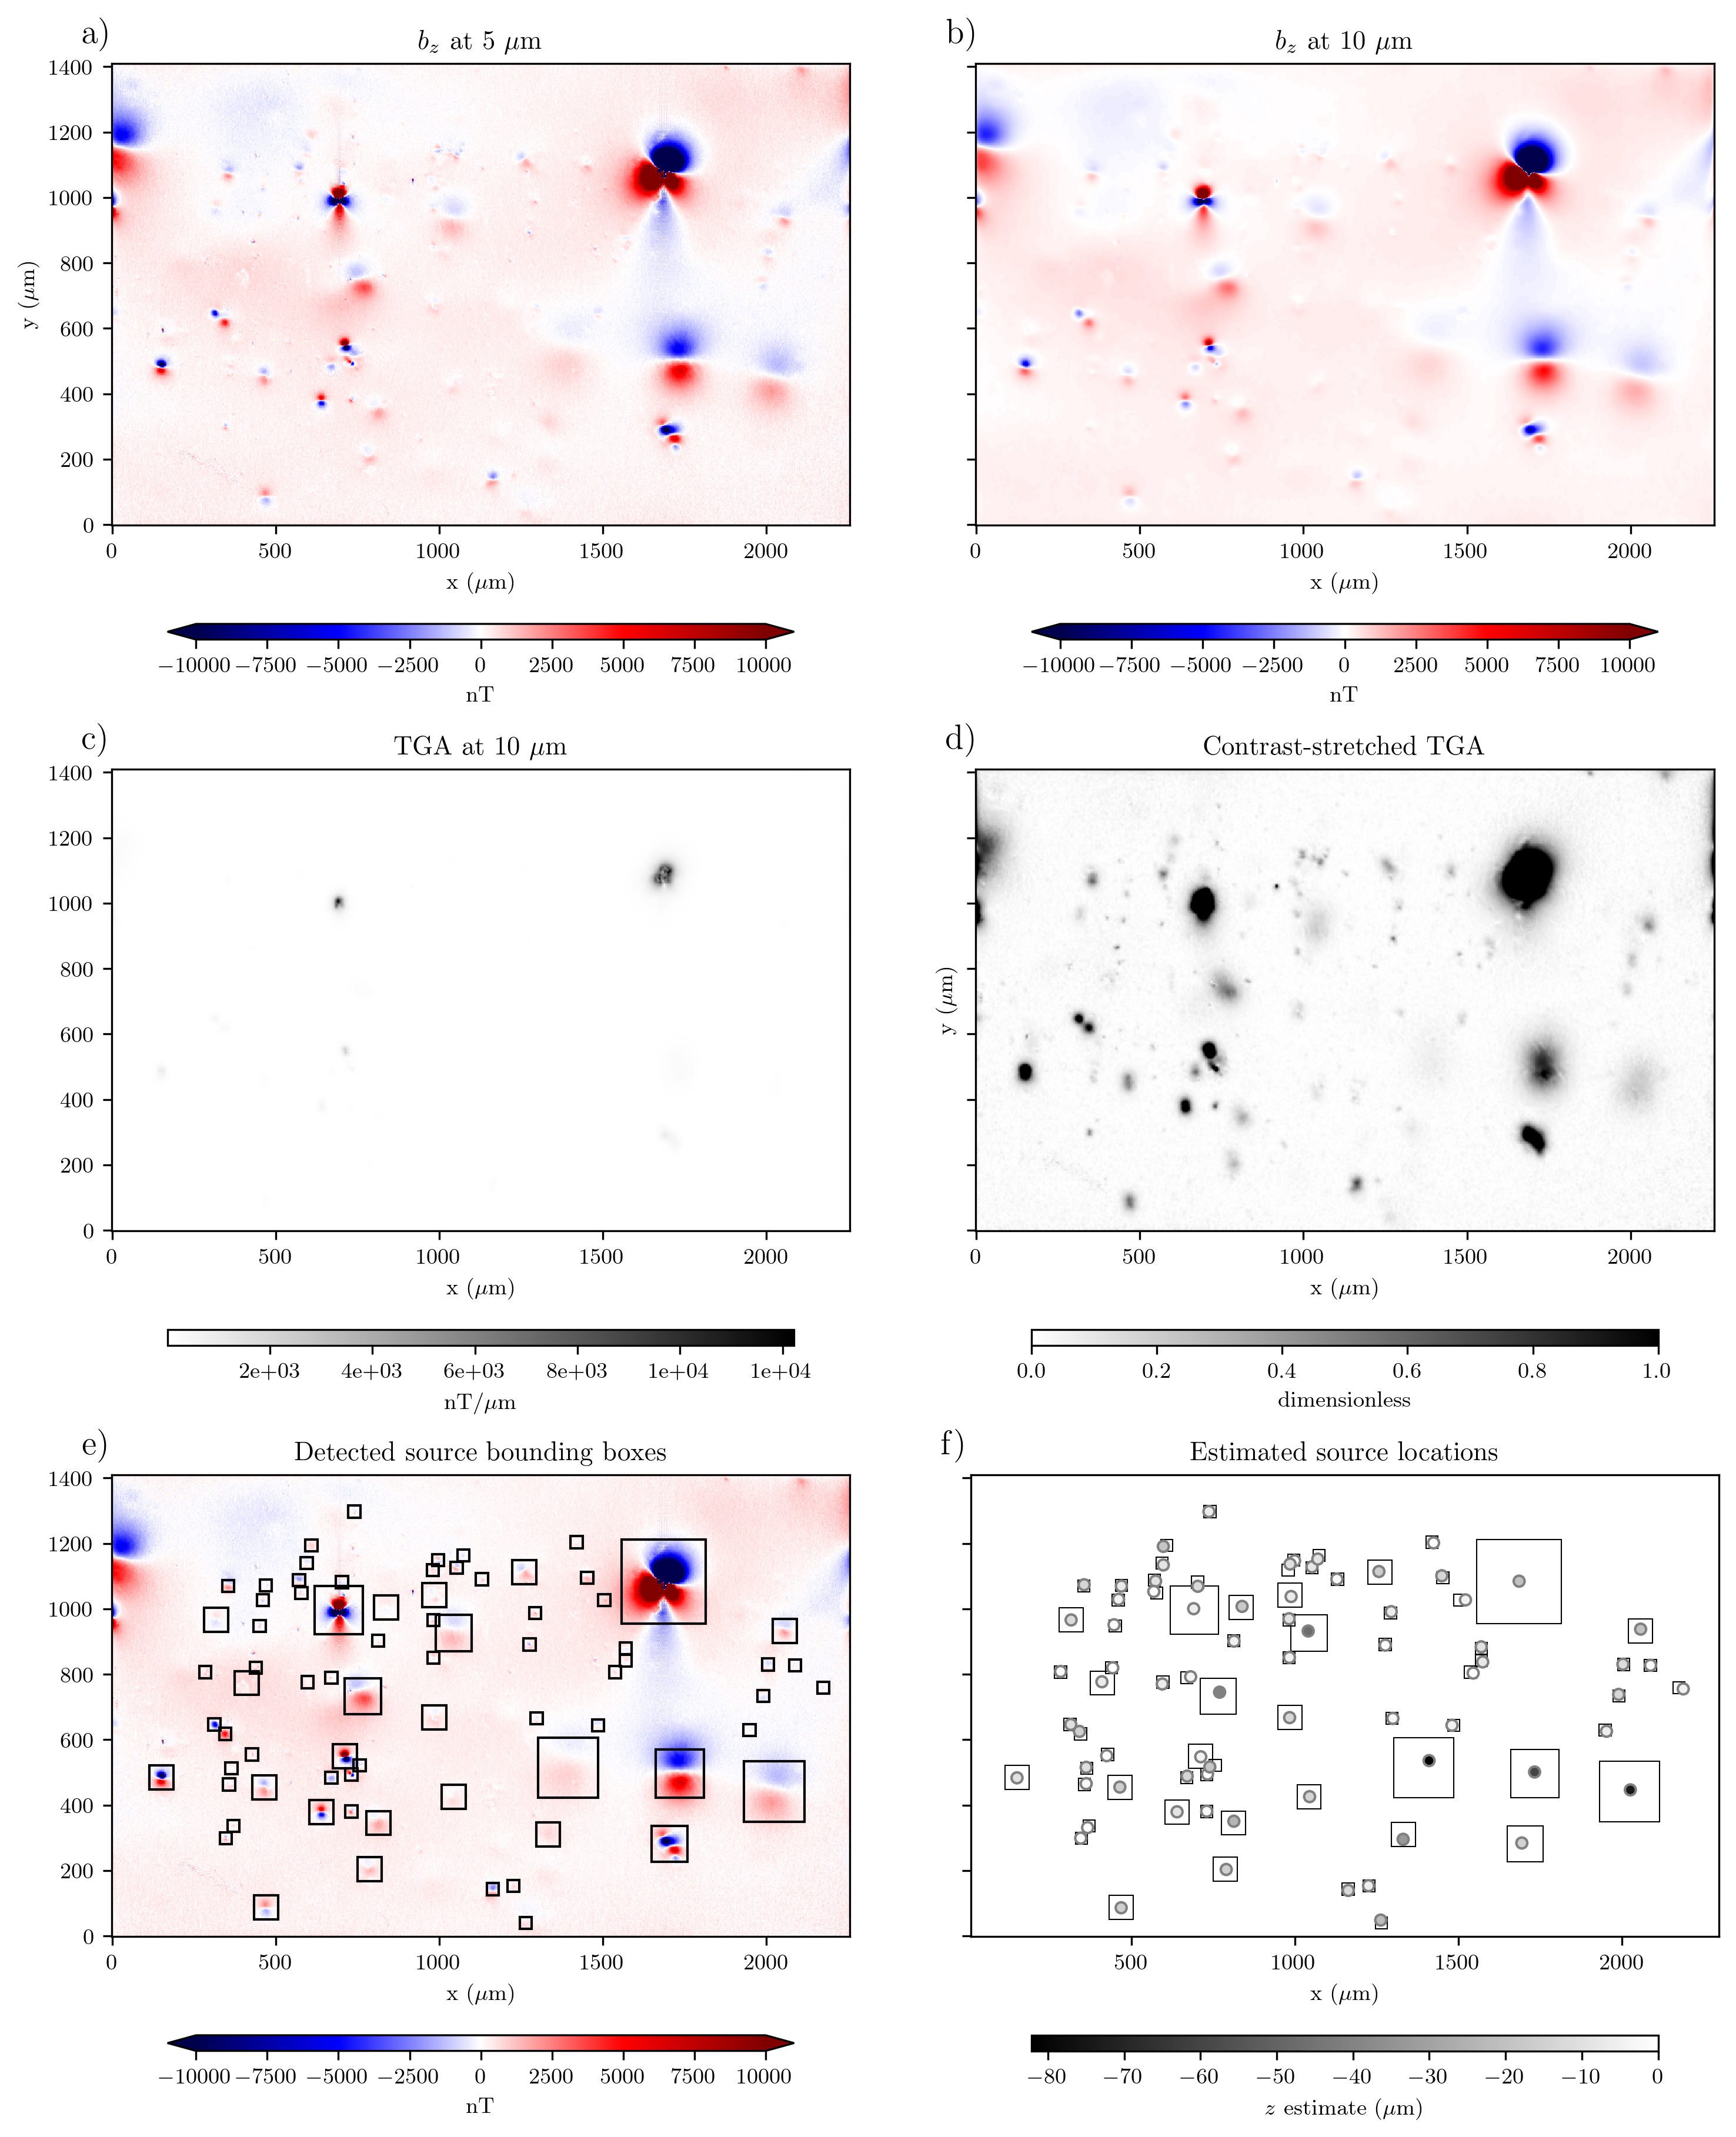
\includegraphics[width=1\linewidth]{micromag-euler-dipole/figures/real-data.png}
\caption{Real data and the various processing steps performed prior to the dipole moment inversion.
    a) The real sample vertical component magnetic data $b_z$ observations at
    $z = \qty{5}{\um}$.
    b) Anomaly map after upward-continuation to $z = \qty{10}{\um}$ to attenuate short-wavelength noise.
    c) The total gradient amplitude (TGA) calculated from the
    upward-continued data.
    d) The contrast-stretched TGA.
    e) The detected source bounding boxes (black squares) that correctly
    encapsulate the main signal of the sources.
    f) The estimated source locations (colored circles) from Euler
    Deconvolution of the upward-continued data inside each bounding box.
    The color represents the estimated $z$ coordinates.
  }
\label{real-data}
\end{figure}

After remanence acquisition, we performed a magnetic map with the Quantum
Diamond Microscope (QDM) at Harvard University over a sample section of
approximately $\qty{1410}{\um} \times \qty{2256}{\um}$ (Figure~\ref{real-data}a) with a grid
spacing of \qty{2.35}{\um} and a sensor-sample distance of approximately \qty{5}{\um}, totaling
576,000 data points. The QDM is housed in a shielded room, in
order to avoid the influence of the Earth's magnetic field while the data were taken in projected magnetic microscopy mode and converted to the vertical component of magnetic field ($b_z$) using a spectral approach \citep{Lima2009, Fu2020,
Glenn2017}. We applied a bias field of \qty{0.9}{\milli\tesla} during the measurement, which was periodically reversed to result in an effective background field of $< \qty{1}{\micro\tesla}$.  After applying the magnetic anomaly detection algorithm (Figure~\ref{real-data}b-e), it was
possible to determine the windows for 100 potential sources, of which 75 remain after filtering for coherent Euler deconvolution position ($z_c \leq 0$), as shown in Figure~\ref{real-data}e.

\begin{figure}[tb!]
\centering
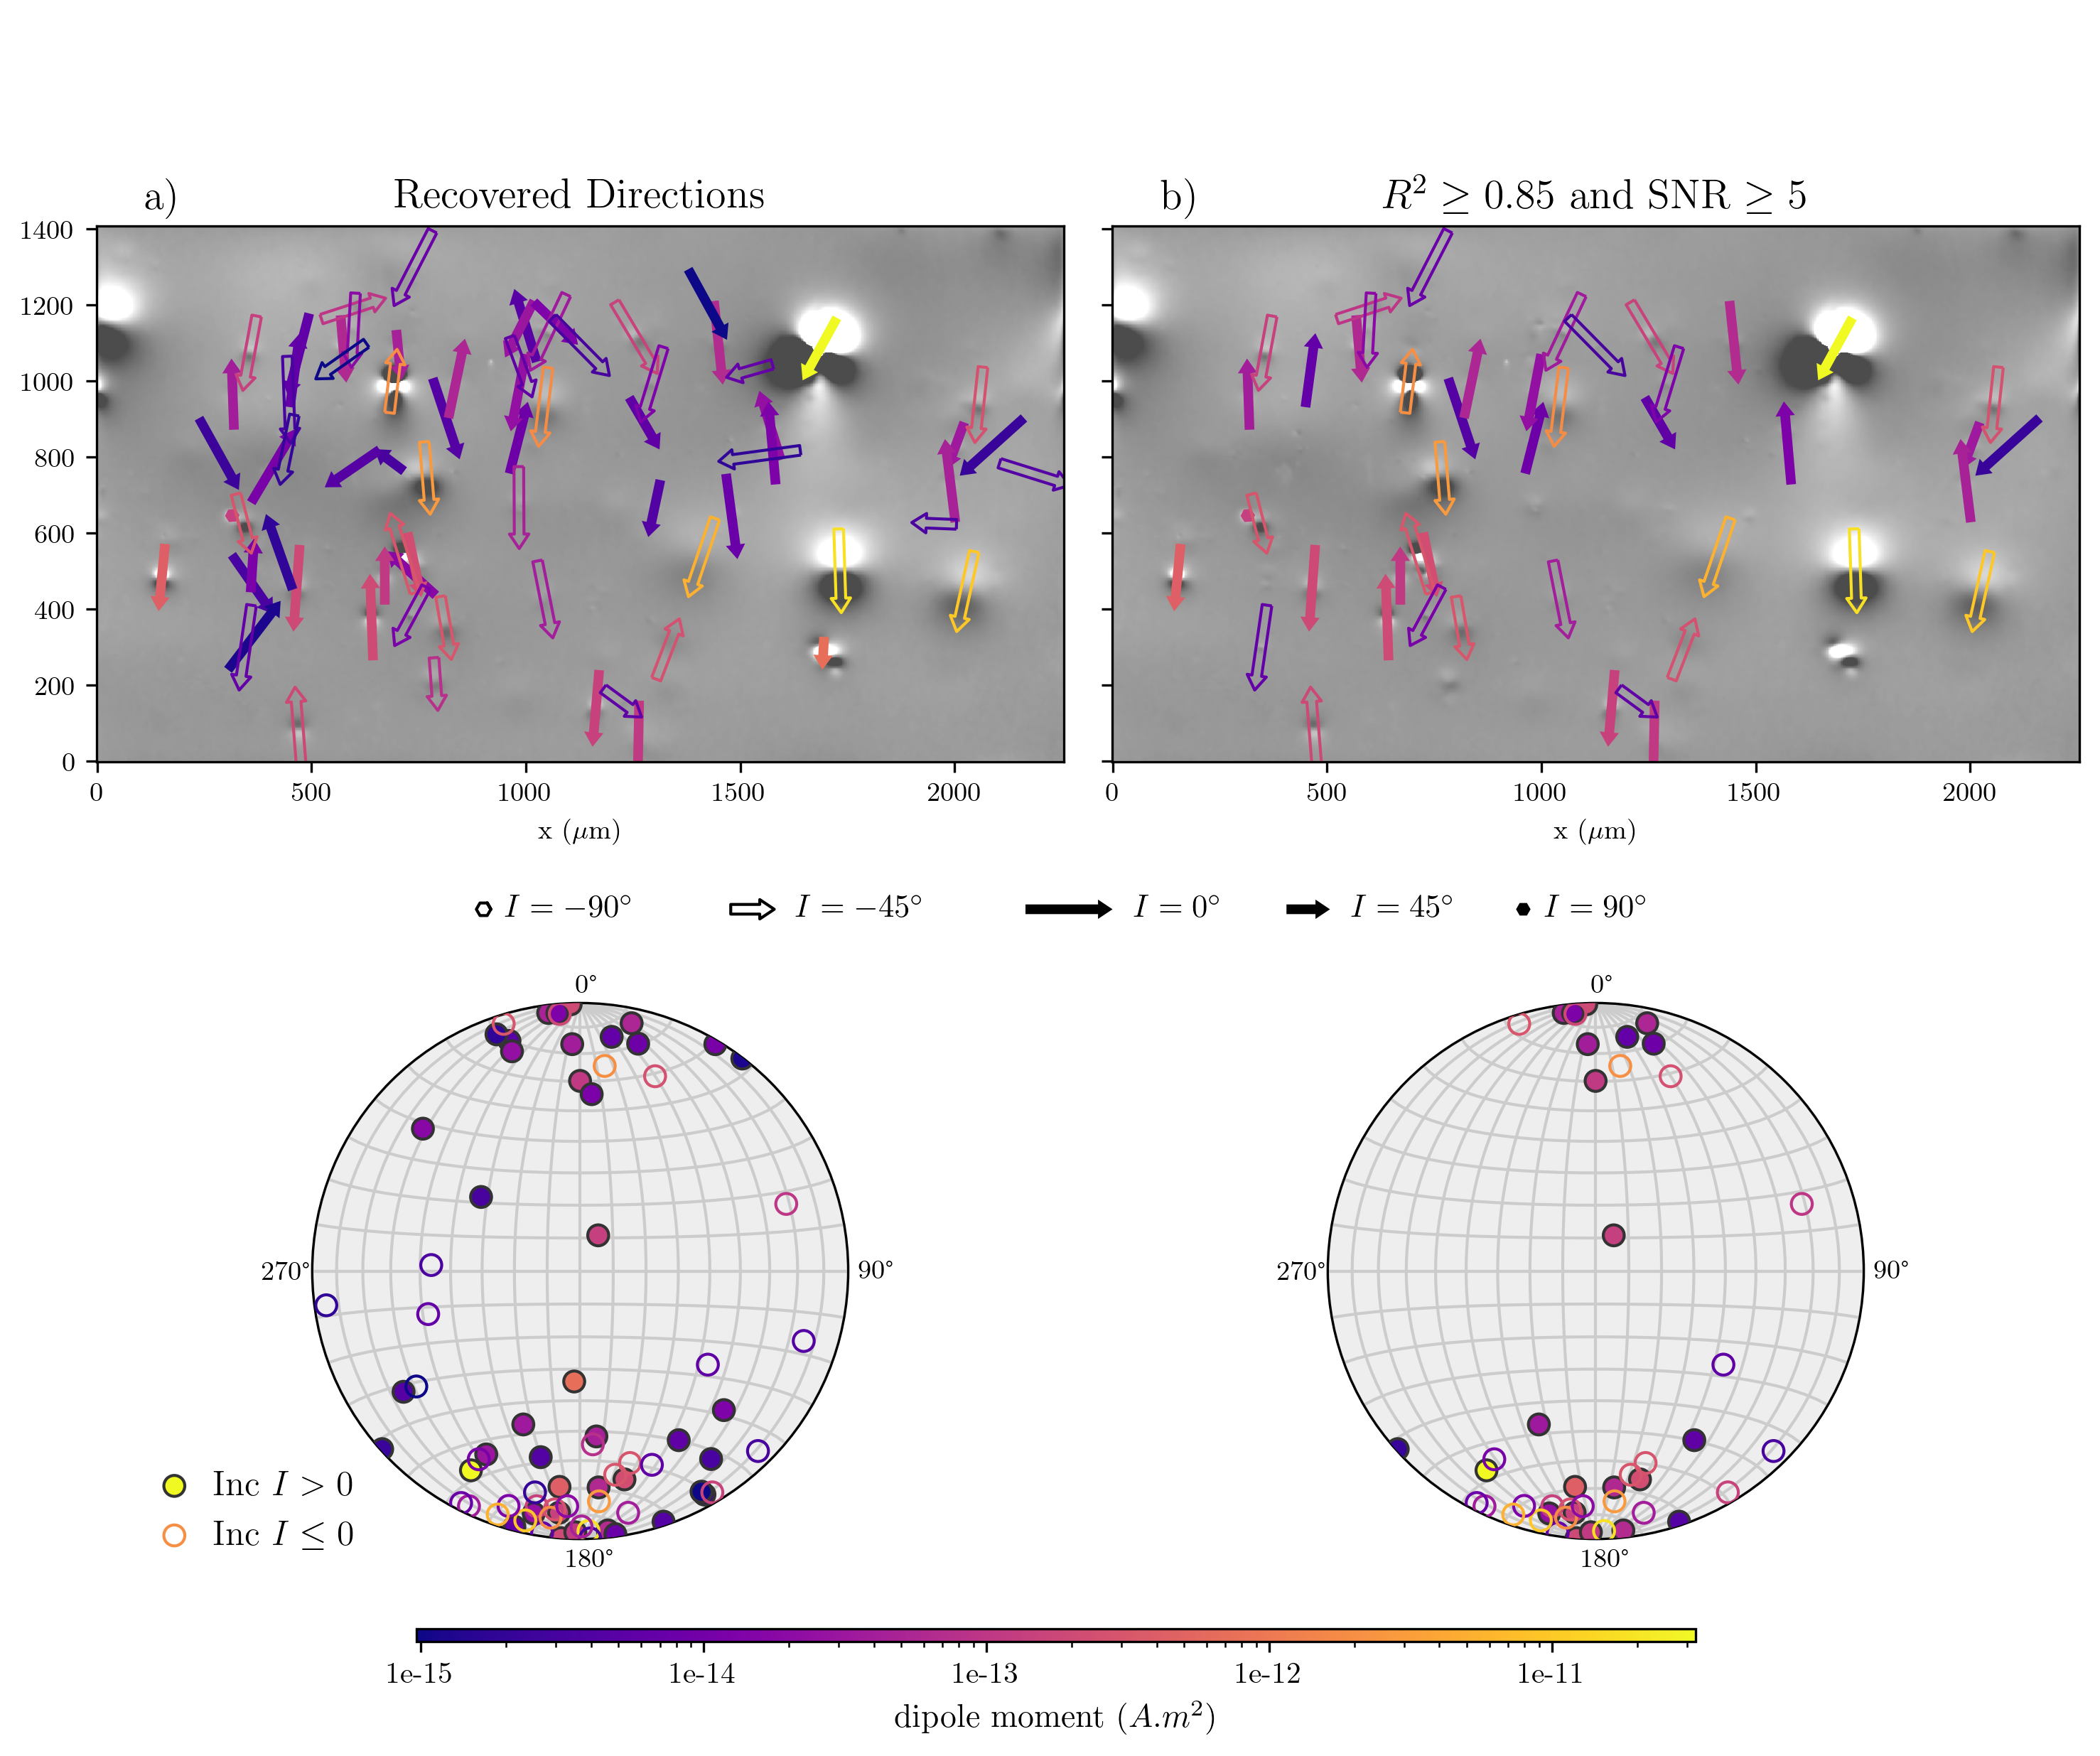
\includegraphics[width=1\linewidth]{micromag-euler-dipole/figures/real-data-stereograms.png}
\caption{
Comparison of the estimated dipole magnetic moments and directions for the real data sample.
a) All estimated directions without filtering ($M=75$). b) Estimated directions filtered ($M=46$) by the coefficient of determination ($\geq 0.85$) and SNR ($\geq 5$), which shows two clusters of direction located on each pole of the stereogram.
}
\label{real-data-stereograms}
\end{figure}

In order to reduce the computation time, the Euler deconvolution and magnetic moment inversions were done within each data window, instead of solving all sources parameters at the same time. We obtained the position and dipole moment for all 75 magnetic grains (Figure~\ref{real-data-stereograms}a). Then, we calculated the residuals of the inversions in each window and subsequently the coefficient of determination $R^2$ and signal-to-noise ratio (SNR), which were parameters used as filters for the best directions obtained. We considered a good fit to be achieved when $R^2$ was greater or equal to 0.85 and SNR was greater than 5. An $R^2$ value of 0.85 indicates that \qty{85}{\percent} of the measured magnetic data is explained by the predicted dipole model, which is equivalent to the dipolarity test approach \citep{Fu2020}. On the other hand, an SNR of 5 means that the dipolar signal is 5 times greater than the residual noise. By using these criteria, we ensured that the fit was sufficiently accurate and the dipole model provided a reliable approximation of the original magnetic data. About 46 identified sources passed these criteria. This filtering technique removed the models with poor fit to the data, which includes the ones that were too corrupted with noise. The filtered results show more clearly the expected directional clusters of hematite and magnetite crystals (Figure~\ref{real-data-stereograms}b). Notably, it is confirmed that the sample has both magnetic minerals, but by the expected directions we can also stipulate that the magnetite grains outnumber the hematite ones.

%%%%%%%%%%%%%%%%%%%%%%%%%%%%%%%%%%%%%%%%%%%%%%%%%%%%%%%%%%%%%%%%%%%%%%%%%%%%%%%
\section{Discussion}

Since the pioneering work of \cite{Egli2000}, many methodologies were proposed for solving the inverse problem of micromagnetic data and, for the purpose of comparison, we separate them into two categories based on the main estimated parameter by the inversion procedure.
In the first type of approach, the main goal is usually to estimate an average magnetization by inverting for the superficial magnetization of the whole sample, commonly by assuming unidirectional or uniform magnetization \citep[\textit{e.g.},][]{Weiss2007}.
There have been significant efforts to enhance the performance of such methods in the spatial domain \citep[\textit{e.g.},][]{Myre2019} and the frequency domain  \citep[\textit{e.g.},][]{Lima2013}.
This methodology can be used to estimate the average magnetic direction and the total moment direction with the assumption that the particles were all magnetized in the direction of the same induced field \citep[sIRM and/or NRM in basalts,][]{Weiss2007}.
However, this assumption is not always true when dealing with complex samples (\textit{i.e.}, more than one stable direction), which leads to the same drawbacks as the classic paleomagnetic measurements using bulk samples.
The second type of approach has the goal of finding the magnetic properties of individual sources, which can be done by either inverting the dipole moment of a single source within a cropped section of an upward continued anomaly map \citep[\textit{e.g.},][]{Lima2016, Fu2020} or by the insertion of additional information of the sources’ shape, such as micro-computed tomography (microCT) \citep[\textit{e.g.},][]{Fabian2019, DeGroot2018, DeGroot2021, Koster2023}.
The latter further allows unique estimation of magnetic moment configuration of even higher orders components through a spherical harmonic expansion constrained by micromagnetic models \citep[\textit{e.g.},][]{CortesOrtuno2021, CortesOrtuno2022}.
Such techniques come with some difficulties, such as having to manually select the data for inversion or dealing with the limitations of the tomography methods.
For example, microCT provides high-resolution imaging of internal structures, but it is accompanied by some limitations when it comes to paleomagnetic studies in particular. The technique has a spatial resolution on the order of a few micrometers, which is not sufficient to directly image the fine-grained single-domain magnetites \citep{DeGroot2018}.
The microCT also struggles to discern ferromagnetic (\textit{l.s.}) from non-magnetic/antiferromagnetic minerals, as pointed out by \cite{DeGroot2021}, since they usually have similar densities and therefore similar X-ray attenuation \citep{Cnudde2013},  though the subsequent inversion may assign to them negligible magnetization.
In any case, the major limitation of microCT lies in the trade-off between the resolution and the sample size, requiring small sample volumes to achieve higher resolutions causing the technique to be too time-consuming.

The methodology proposed here aims to add additional position information to constrain the dipole moment inverse problem without requiring external, expensive, and time-consuming data acquisitions. We also seek to automate as much of the processing as possible to allow large-scale applications of magnetic microscopy, which will be required if it is to be used routinely in paleomagnetic studies.
Below, we discuss the strengths and limitations of each aspect of the proposed methodology in light of the various synthetic data tests that were performed.

\subsection{TGA-guided windows: magnetic source detection using LoG Kernel}

Our proposed methodology has the goal of finding each individual source’s dipole moment components without the trouble of manually selecting cropped data or needing any type of additional information.
To better examine its advantages and disadvantages, we first need to point out the strengths and weaknesses of the technique used in the detection of sources, the Laplacian of Gaussian (LoG) kernel \citep{Marr1980}.
The LoG is a computer imaging technique that is able to identify regions where the intensity changes abruptly by convolving the image with the LoG filter, and is the result of the combination of the Gaussian blur and Laplacian filter \citep{gonzalez2018}.
The Laplacian filter is able to highlight the regions where the intensity changes rapidly.
On the other hand, the Gaussian blur is a smoothing filter for high-frequency noise, which reduces the likelihood of generating artifacts.
Hence, the result of this LoG operation can identify blobs as regions above a certain threshold, this threshold crossing determines what are brighter spots (local maxima) surrounded by a darker background.
It is also scale-invariant by detecting blobs of different sizes and intensities, a feature achieved by varying the sizes of the Gaussian filter.
The advantages of the methodology are (i) high-accuracy blob detection; (ii) scale-invariant for images with different intensities/sizes of objects; while also being (iii) robust to the presence of noise due to the Gaussian smoothing filter.
While the main drawbacks of the LoG blob algorithms are: (i) being computationally expensive/time-consuming when dealing with larger images and (ii) the requirement of parameter adjustments, such as the threshold and the kernel sizes.

We consider the total gradient amplitude (TGA) to be the ideal input for the LoG blob detection algorithm for potential field studies (micro and/or macroscale).
The TGA highlights the subsurface sources by generating a map that is entirely positive and where the signal is concentrated on top of the sources.
This technique is widely used in aeromagnetic surveys to aid in mapping the boundaries of sources.
The windows generated from the TGA map isolate the main magnetic signal for each source. This guarantees that both Euler deconvolution and dipole moment inversion are performed using the most important parts of the signal, balancing accurate parameter estimation and fast run-time due to the use of fewer data points.

While the windows approach violates the fundamental theory of the inversion problem that requires the sampled area to be finite and encapsulated by the inversion domain to ensure the uniqueness of results \citep{Baratchart2013, Lima2013}, our results do not present any practical issues and are able to correctly recover the position and dipole moment of the sources, even with slightly truncated data.
Our technique is similar to the one reported by \cite{Weiss2007},
which involves thresholding the long-distance interaction
of each dipole in the SMM data, which excludes the effect of other dipoles by setting their contribution to zero, resulting in a sparse matrix that permits faster calculations.
In contrast to this approach, we apply the source detection to a TGA map, which concentrates the signal above each particle, to select the windows that isolate the area containing the main signal of the desired dipole. The area out of the boundaries of the window is less sensitive to variation in the magnetic parameters of the source, hence we may exclude them from the inversion domain without ill effects.
This technique allows us to obtain the 3D position and an approximation of the dipole moment components of hundreds of sources in a computationally efficient way.
In fact, the main time bottleneck of our methodology is not the inversion but the source detection process.

Another main limitation arises from the spatial constraints inherent to our approach. Specifically, the blob detection struggles when dealing with sources that are closely spaced or overlapping, in the last case, it is unable to discern the magnetic sources. Through multiple tests (Figure~\ref{detection-map}), we have found that, for shallow sources, with sensor-sample height $\leq \qty{5}{\um}$, a minimum separation distance of approximately \qty{14}{\um} is necessary to achieve successful source detection. This distance steadily increases for deeper seated sources, requiring around \qty{20}{\um} of separation for the sensor-sample height of \qty{25}{\um}. This immensely impacts the algorithm's detection capacity, as the particle count escalates, there is a persistent decline in the rate of successful source detection, as shown in Figure~\ref{grain-concentration}a. In essence, the algorithm's effectiveness diminishes as sources become more densely packed, posing a challenge in scenarios where particle density is high (\textit{e.g.}, extrusive rocks). On the other hand, as shown in our complex synthetic and real rock samples the technique could be densely applied to rocks with a lower concentration of magnetic grains (\textit{e.g.}, carbonates), due to its high successful rate for detection of sources.


\subsection{Critical assessment of source position determination}

Working with potential field data is challenging due to the ambiguity inherent to data modeling. To obtain unique and reliable results from data inversion, it is necessary to provide as much prior information as possible.
One way to circumvent the ambiguity is to incorporate prior information about the subsurface structure, such as the position of the source of magnetization.
\citet{Oliveira2015Estimation} showed that the magnetization direction recovered by a least-squares inversion with a spherical approximation is sensitive to variations in the horizontal coordinates of the center of the magnetic sources, but is practically insensitive to variations in depth.
They propose the Euler deconvolution method as an adequate technique to estimate the central positions that will be used as prior information for inversion.
This occurs mainly because the recovery of the source's horizontal coordinates is considerably accurate, while the vertical coordinate can undergo greater variation even though it still provides satisfactory results \citep{Silva2003, Melo2013}.
This remark is also better observed in our simple synthetic sample where the estimated horizontal positions are close to the true values, which implies small misfit values in the recovered magnetic directions.
Although the estimated magnetic moment amplitude for said sample is satisfactory, this parameter is more affected by the variations in the depth of the source due to the inherent ambiguity between depth and moment amplitude.

Despite using a structural index $\eta = 3$ for the Euler deconvolution (indicating dipolar sources) , the technique did not present significant difficulties in estimating the 3D position of non-dipolar sources for source-sensor separations higher than around \qty{2.5}{\um} (Figure~\ref{non-dipolarity-synthetic-data-positioning}). This adaptability allows for an extension of its application to magnetic particles with a strong influence of higher-order magnetic anomalies.
Lastly, as shown in the complex synthetic sample, the Euler deconvolution can reliably estimate the position of well-individualized sources. When dealing with clustered particles, however, the Euler deconvolution solutions start to deviate from the true positions. This deviation is particularly notable in the z-coordinate, which is shown by \cite{Oliveira2015Estimation} to not affect the magnetization direction estimation, but can negatively influence the dipole moment amplitude estimation.

In summary, Euler deconvolution must ideally be executed within a data window containing only one magnetic source and the lowest amount possible of noise in order to accurately estimate the source position. We have shown that our method is able to satisfy these conditions for a decent amount of sources by upward-continuation of the data prior to derivative calculation and by use of the source detection method.

\subsection{Critical assessment of dipole moment approximation}
\label{dipole-reliability}

Our approach relies on the premise of assuming the magnetic anomaly within
the data window is a response of a dipolar source.
The latter is true when working
with particle signals in the single domain state since they are uniformly magnetized particles \citep{Dunlop1997} with strong dipolar anomalies.
However, \cite{Nagy2017} reported that particles within the pseudo-single domain state can record the paleomagnetic field for longer periods of time than single domain ones, but also present strongly non-dipolar characteristics.
Hence, the application of the proposed algorithm in natural samples is expected to be unsuccessful in states other than the single domain state unless sources are sufficiently far from the sensor to be approximated by dipoles. In instances where sources exhibit strong higher-order magnetic anomalies, such as quadrupole or octupole \citep[\textit{e.g.},][]{CortesOrtuno2021}, even at larger source-sample separations, the dipole model fitting process may not yield satisfactory results. Consequently, the presence of strong higher-order anomalies within the magnetic sources can impact the accuracy of our inversion results.

\cite{CortesOrtuno2022} showed that PSD state particles present more accurate inversion results when considering the non-dipolar components for small sample-sensor distances (\textless 1 $\mu$m). For larger sensor distances, the dipole as approximations are remarkably accurate, as the higher-order moments decay rapidly with distance and therefore have less
influence on the particle's magnetic signal.
Thus, our approach can be considered reasonable to work with both particle SD and PSD state signals.
The latter happens mainly due to the sensor height being usually greater than \qty{5}{\um} for QDM data. Considering a particle on the immediate surface of the sample the higher-order moments are already quite attenuated, thus circumventing the prominent problems described for non-dipolar components. This is corroborated by our non-dipolar synthetic sample showing the almost complete attenuation of non-dipolar components at distances greater than \qty{5}{\um}.

Despite the excellent signal-to-noise ratio that the SMM provided with the
proximity of the sensor to the sample, it is worth mentioning that the
measurement noise can still overshadow the responses of very weak/small, or
deep particles, generating unreliable inversion results.
Therefore, it is necessary to verify that the inversion reached a satisfactory prediction, such as the coefficient of determination \citep[dipolarity test, ][]{Fu2020} and the
signal-to-noise ratio suggested by \cite{CortesOrtuno2021}. This filtering process is better observed in the complex synthetic data where it becomes evident the direct relationship between the poorly estimated dipole moment and direction with the lowest values for both $R^2$ and SNR scores (Figure~\ref{complex-synthetic-comparison}).

%%%%%%%%%%%%%%%%%%%%%%%%%%%%%%%%%%%%%%%%%%%%%%%%%%%%%%%%%%%%%%%%%%%%%%%%%%%%%%%
\section{Conclusion}

We developed an efficient semi-automated method to determine the position and dipole moments of dipolar sources on a microscale.
The method is an advancement towards the application of magnetic microscopy to paleomagnetic studies using thin sections.
A possible application is the isolation of the responses of more reliable recorders of the Earth's geomagnetic field from those of less reliable ones.

We also present a new way to solve the Euler deconvolution problem for determining the position of magnetic anomaly sources. Instead of the traditional moving window approach, we select data windows based on the Laplacian of Gaussian method applied to total gradient amplitude maps.
In this way, each window will ideally contain a single source and we are able to reduce the usually numerous spurious solutions to just a single solution per source.
This approach could also be adapted for traditional aeromagnetic data studies in cases where the sources are approximately spherical or only slightly elongated.
The source detection method is able to correctly isolate sources that are at
least \qty{15}{\um} apart for a source-sensor separation of \qty{5}{\um}.
For grain concentrations of 6250 grains/mm³, our method is
able to detect over 60\% of the particles present in the data.

To recover the dipole moment, we assume that there is one source for each data window, that its central position is known (through Euler deconvolution), and that its magnetization is uniform.
This last premise aligns with magnetically stable SD particles and with PSD ones at a reasonable sensor-sample separation, which is the basis of classical paleomagnetism.
Also, there is no need for any prior knowledge other than the observed magnetic anomaly and the structural index of the sources (which is related to the dipolar approximation).
Therefore, this method can be quickly applied to a set of thin sections of rocks to obtain the distributions of magnetic directions of each source identified in the sample.

The test using a simple synthetic sample shows the capability of the method by estimating not only the precise center positions but also retrieving the magnetization directions and intensity for both dipolar and non-dipolar sources, even under the effect of high-frequency noise.
The test on a more complex synthetic sample highlights the applicability of the method in datasets resembling those obtained from speleothems.
The data are more complex with varied magnetization directions and intensity, in addition to also taking into account the high and low-frequency noise and sources with variable dipole moment intensities and depths.
The application to a real speleothem dataset positively answered the question of the algorithm's ability to deal with the real-world signals and noise.
It also showed the capacity of retrieving different magnetization directions recorded by magnetic minerals with different coercivities and magnetic signal intensity disparities.
We also assessed the quality of the fit between the predicted dipole model and the original magnetic data using two criteria: the coefficient of determination ($R^2$) and the signal-to-noise ratio (SNR).

We expect that this method can be widely applied to magnetic microscopy studies involving particles in the SD and PSD domains, particularly where grain concentrations are at or below 6000-10000 grains/mm³. The method can be applied in full as presented here or its individual components (source detection, Euler deconvolution, dipole moment inversion) can be combined with existing or future methods. There are still issues to be overcome with regard to situations where the signal of two or more sources overlap significantly, when non-dipolar effects are strong even at larger source-sensor separations, and how to best combine and benchmark the inversion results against microCT and micromagnetic modeling studies.

%%%%%%%%%%%%%%%%%%%%%%%%%%%%%%%%%%%%%%%%%%%%%%%%%%%%%%%%%%%%%%%%%%%%%%%%%%%%%%%
\section*{Open Research}

The Python source code used to produce all results and figures presented here, as well as supplemental figures and Jupyter notebooks, are available from \citet{sourcearchive}, which can also be found on \url{https://github.com/\GitHubRepository} under the MIT and CC-BY licenses.
The QDM magnetic microscopy data are available
from \citet{janinedata} under the CC-0 license.

The image re-scaling and blob detection through the Laplacian of Gaussian
method were performed with the scikit-image library \citep{VanderWalt2014}.
We also used matplotlib \citep{Hunter2007} and mplstereonet \citep{mplstereonet}
for generating figures and stereograms.
Basic calculations were performed using Numpy \citep{numpy} and Scipy
\citep{scipy}.
Verde \citep{verde2018} was used to generate data grids.
Upward continuation was performed using Harmonica \citep{harmonica2020}.
The Choclo library \citep{choclo2022} provided kernel functions used in the
forward and inverse problems.
The Numba just-in-time compilation library \citep{numba2015} was used to
speed-up calculations.
Lastly, the xarray library \citep{xarray} offered a fast and powerful
tool for working with multi-dimensional datasets allowing an easy way of data
visualization and extraction with advanced indexing techniques.


%%%%%%%%%%%%%%%%%%%%%%%%%%%%%%%%%%%%%%%%%%%%%%%%%%%%%%%%%%%%%%%%%%%%%%%%%%%%%%%
\section*{Acknowledgements}

The authors would like to thank the editor Joshua Feinberg and two anonymous reviewers for their contributions which greatly improved our paper. We are indebted to the developers and maintainers of the open-source software
without which this work would not have been possible.
This research was supported by
grant 162704/2021-6 from the Conselho Nacional de Desenvolvimento Científico e Tecnológico (CNPq),
grant 2021/08379-5 from the Fundação de Amparo à Pesquisa do Estado de São Paulo (FAPESP),
grant PRPI 22.1.09345.01.2 from Universidade de São Paulo,
and grant IES\textbackslash{}R3\textbackslash{}213141 from the Royal Society.
The opinions, hypotheses, and conclusions or recommendations expressed in this
material are the responsibility of the authors and do not necessarily reflect
the views of FAPESP.

\endgroup

%==============================================================================
\chapter{Iterative magnetic microscopy inversion}

\begingroup
%%%%%%%%%%%%%%%%%%%%%%%%%%%%%%%%%%%%%%%%%%%%%%%%%%%%%%%%%%%%%%%%%%%%%%%%%%%%%%%
% Set variables with the title, authors, etc.
\newcommand{\Title}{Robust directional analysis of magnetic microscopy images using non-linear inversion and iterative Euler deconvolution}
\newcommand{\TitleShort}{A robust iterative method for magnetic microscopy inversion}

\newcommand{\Year}{2025}
\newcommand{\PreprintOn}{2025/03/28}
\newcommand{\PreprintRevAOn}{2025/04/03}
\newcommand{\SubmittedOn}{2025/04/03}
% \newcommand{\PublishedOn}{2023/02/28}

\newcommand{\AuthorShort}{Souza-Junior \textit{et al.}}
\newcommand{\Authors}{%
  Gelson F. Souza-Junior\textsuperscript{1,2},
  Leonardo Uieda\textsuperscript{1},
  Ricardo I. F. Trindade\textsuperscript{1},
  Roger R. Fu\textsuperscript{2},
  Ualisson D. Bellon\textsuperscript{3}
  and
  Yago M. Castro\textsuperscript{1}
}
\newcommand{\Email}{gelson.ferreira@usp.br}
% \newcommand{\Email}{gferreiradesouzajunior@fas.harvard.edu}
\newcommand{\Corresponding}{%
  Corresponding author: Gelson F. Souza-Junior <\href{mailto:\Email}{\Email}>
}
\newcommand{\Affiliations}{%
  \textsuperscript{1} Universidade de São Paulo, Brazil;
  \textsuperscript{2} Harvard University, USA;
  \textsuperscript{3} University of Edinburgh, UK.
}

\newcommand{\Journal}{JGR: Solid Earth}
\newcommand{\JournalDOI}{YYYYY/YYYYYYY}
\newcommand{\PreprintDOI}{10.31223/X5N42F}
\newcommand{\ArchiveDOI}{10.5281/zenodo.15132658}
\newcommand{\GitHubRepository}{compgeolab/micromag-interfering-sources}

\newcommand{\Keywords}{%
  paleomagnetism; magnetic microscopy;
}


\begin{summarybox}
    \noindent
    This chapter was originally published as the preprint
    \textbf{``Souza-Junior, G. F., Uieda, L., Trindade, R. I. F., Fu, R. R.,
    Bellon, U. D. and Castro, Y. M. (\Year). \Title{}. \textit{EarthArXiv}.
    doi:\href{https://doi.org/\PreprintDOI}{\PreprintDOI}.''} under the
    terms of the CC-BY license. It is reproduced here under these terms.
    The preprint is currently under review at \textit{\Journal{}}.
\end{summarybox}

\section*{Abstract}
The first step in scientific data acquisition often involves analyzing entire samples, providing only a general characterization of the material. Enhancing data acquisition by improving spatial resolution and isolating the underlying phenomena contributing to the overall signal has become a central direction in various scientific fields. In paleomagnetism, this advancement is now possible with the advent of magnetic microscopy (MM), whose high spatial resolution and magnetic moment sensitivity allow for imaging samples at the mineral grain scale. In this study, we aim to obtain reliable paleomagnetic directions using only MM data. To achieve this, we apply Euler deconvolution to solve the linear problem and mitigate the non-uniqueness associated with inversion. As an additional step, we refine the recovered parameters using a nonlinear inversion and remove interfering signals between sources to minimize noise. This algorithm was applied to both synthetic and real data and compared to its predecessor. The results from synthetic data demonstrate that this new approach is able to detect weaker sources and produce more accurate grain-level results, which in turn leads to larger datasets and improved statistical characterization of the sample. For real data, we observe that the iterative method was significantly more efficient than its predecessor, successfully retrieving the natural remanent magnetization direction of a basaltic sample with \ang{3} accuracy. This represents a significant step forward in applying MM data to paleomagnetic studies.

% \section{Introduction}

Since the pioneering contributions of \citet{Egli2000}, implementing high-resolution  magnetic microscopy (MM) methodologies to paleomagnetic analysis has become increasingly feasible in paleomagnetic research. This has offered an alternative to conventional paleomagnetic approaches that typically analyze entire, centimeter-scale rock samples. Magnetic microscopy allows better characterization of magnetization heterogeneities, which are usually undetectable by classical paleomagnetic analysis, as the magnetometers measure the contribution of all magnetic carriers in the rock at once. Although MM techniques provide a magnetically resolved perspective to each source, processing the measured field can be very challenging. Potential field data are naturally associated with ambiguities, which generate non-unique solutions during inversion procedures that aim to recover the magnetic moment of these sources \citep{Blakely1996}. A standard routine applied to circumvent the non-uniqueness is integrating prior knowledge about the sources causing the anomaly. X-ray computed tomography (microCT) -- which determines the position of magnetic grains within a sample \citep{Fabian2019} -- is an example of such prior information \citep[\textit{e.g.}][]{DeGroot2018, DeGroot2021, Koster2023}, which can then be incorporated into the inversion of the magnetic moment by using spherical harmonic expansions \citep[\textit{e.g.}][]{CortesOrtuno2021, CortesOrtuno2022}.

Another way to incorporate additional information to the inverse problem without performing new measurements was proposed by \citet{Souza-Junior2024}. Their methodology borrows processing and interpretation techniques of aeromagnetic surveys, such as the Euler deconvolution and field transformations, since the data are similar to magnetic microscopy \citep{Weiss2007}. The methodology was designed for the semi-automatic estimation of position and dipole moments for individual grains and consists of three main steps. First, it combines classic potential field data processing (like total gradient amplitude) with image processing techniques (namely, histogram stretching and blob detection) to identify and isolate the magnetic fields of individual sources into data windows. Next, the 3D position of the source is estimated through the Euler deconvolution method \citep{Reid1990} based on the magnetic microscopy field measurements within each data window. Finally, the 3-component dipole moment vector is obtained using a least-square estimator assuming that a dipolar source causes the magnetic anomaly \citep{Oliveira2015Estimation}. The methodology was originally designed for computational efficiency and stability. However, it infringes on the mathematical premise of inversion theory, which states that the sampled area must be encapsulated by the inversion domain \citep{Baratchart2013, Lima2013}. Thus, more often than not, it fails to account for the mutual interference between sources and shifts in the measured field. This study introduces significant modifications to the method of \citet{Souza-Junior2024} that aim to account for the mutual interference of the sources, as well as any shift in the field. Through refining the window-based approach, the proposed methodology is able to more accurately recover the dipole moments and positions of a larger number of sources than the previous method. We tested the improved method in synthetic and real magnetic microscopy data, showing its applicability to micropaleomagnetic analysis.


%%%%%%%%%%%%%%%%%%%%%%%%%%%%%%%%%%%%%%%%%%%%%%%%%%%%%%%%%%%%%%%%%%%%%%%%%%%%%%%
\section{Methods}

We propose modifications to the methodology of \citet{Souza-Junior2024} to improve its accuracy in scenarios where signals from neighboring particles overlap, causing distortions in the signal of the weaker particles and biasing the source detection and dipole moment inversion results (as shown in Figure~\ref{method-redetection}a). The new method uses the following workflow:

\begin{enumerate}
    \item \textbf{Source detection:} We use the same procedure described in \citet{Souza-Junior2024}, namely calculating the total-gradient amplitude of the magnetic data, histogram stretching, and a blob detection algorithm. This produces a set of data windows that contain the observed signals of individual particles.
    \label{alg:workflow-detection}
    \item \textbf{Sort the data windows} by order of decreasing signal strength and perform the following steps on each window following this order:
    \label{alg:workflow-loop}
    \begin{enumerate}
        \item \textbf{Isolate the data:} Select the portion of the magnetic data that falls inside the current data window. The following steps are performed on this selected dataset.
        \item {Euler:}
        \item \textbf{Linear magnetic moment inversion:} Perform a linear inversion to estimate the dipole moment of the source using the Euler deconvolution solution as prior information to fix the source position.
        \item \textbf{Non-linear inversion:} Unlike \citet{Souza-Junior2024}, we then refine the position and dipole moment estimates by a non-linear inversion using the Nelder-Mead method \citep{Nelder-Mead1965,Gao2010}. The Euler deconvolution and linear inversion results are used as initial estimates for the optimization.
        \item \textbf{Signal removal:} Forward model the magnetic field of the estimated dipole from the previous step and remove the signal from the full magnetic data.
    \end{enumerate}
    \item Now, the original magnetic data has been stripped of the signal of all detected sources. Repeat steps~\ref{alg:workflow-detection} and \ref{alg:workflow-loop} on the stripped dataset to detect new sources and determine their positions and dipole moments.
\end{enumerate}

\noindent
Below, we describe these steps in more detail.

\subsection{Position estimation}
    Euler deconvolution (ED) \citep{Reid1990} is a procedure widely applied in aeromagnetic surveys \citep{Barbosa2011, Melo2013} to obtain a 3D position estimation of the magnetic source. The only assumption is the source's shape given by the structural index ($\eta$).
    In the case of a dipole $\eta = 3$. Euler deconvolution is based on Euler's homogeneity equation

        \begin{equation}
        \label{eq_euler_homogeneity}
        (x - x_c)\partial_x f
        + (y - y_c)\partial_y f
        + (z - z_c)\partial_z f
        = (b - f)\eta
        \ ,
        \end{equation}

    \noindent
    in which $(x, y, z)$ are the observation point coordinates in a Cartesian system, $(x_c, y_c, z_c)$ are the coordinates of the source, $b$ is a constant shift in the data called the \textit{base level}, $\eta$ is the structural index, and $f$ is the magnetic field.
    The equation above can be rearranged to isolate the unknown source position  and the base level

    \begin{equation}
    x_c \partial_x f + y_c \partial_y f + z_c \partial_z f + \eta b
    =
    x \partial_x f + y \partial_y f + z \partial_z f + \eta f
    \ .
    \end{equation}

    Given $N$ observation of the magnetic field and its $x$-, $y$-, and $z$-derivatives, we can form a $N \times 4$ system of equations

    \begin{equation}
    {\overbrace{
    \begin{bmatrix}
      {\partial_x f}_1 & {\partial_y f}_1 & {\partial_z f}_1 & \eta \\
      {\partial_x f}_2 & {\partial_y f}_2 & {\partial_z f}_2 & \eta \\
      \vdots & \vdots & \vdots & \vdots \\
      {\partial_x f}_N & {\partial_y f}_N & {\partial_z f}_N & \eta
    \end{bmatrix}
    }^{\mathbf{G}}}_{N \times 4}
    {\overbrace{
    \begin{bmatrix}
      x_c \\ y_c \\ z_c \\ b
    \end{bmatrix}
    }^{\mathbf{p}}}_{4 \times 1}
    =
    {\overbrace{
    \begin{bmatrix}
      x_1 {\partial_x f}_1 + y_1 {\partial_y f}_1 + z_1 {\partial_z f}_1 + \eta f_1 \\
      x_2 {\partial_x f}_2 + y_2 {\partial_y f}_2 + z_2 {\partial_z f}_2 + \eta f_2 \\
      \vdots \\
      x_N {\partial_x f}_N + y_N {\partial_y f}_N + z_N {\partial_z f}_N + \eta f_N \\
    \end{bmatrix}
    }^{\mathbf{h}}}_{N \times 1}
    \ ,
    \end{equation}

    \noindent
    in which $\mathbf{G}$ is the Jacobian matrix, $\mathbf{p}$ is the parameter vector, and $\mathbf{h}$ is the pseudo-data vector.

    The least-squares solution of this linear system is defined by the vector $\mathbf{p}$ that minimizes the misfit function, $\phi(\mathbf{p})$, given by the sum of the squared differences between the observed pseudo-data vector $\mathbf{h}^o$ and the predicted pseudo-data vector $\mathbf{h}$

    \begin{equation}
    \label{function_phi}
    \phi(\mathbf{p})
    = \| \mathbf{h}^o - \mathbf{h} \|_2^2\
    = \| \mathbf{h}^o - \mathbf{G}\mathbf{p} \|_2^2\
    \ .
    \end{equation}

    \noindent
    The solution that minimizes the misfit function is

    \begin{equation}
    \label{euler_solution}
    \mathbf{p} = \left(\mathbf{G}^T \mathbf{G}\right)^{-1} \mathbf{G}^T \mathbf{h}^o\ .
    \end{equation}

    \noindent
    The parameter vector $\mathbf{p}$ contains the coordinates of the dipolar source $(x_c, y_c, z_c)$, as well as the base level $b$, which is the background field within the data window.

\subsection{Linear magnetic moment inversion}

     Following \citet{Oliveira2015Estimation} and \citet{Souza-Junior2024}, the vertical component of the magnetic field $f_z$ has a linear relationship with the dipole moment components $(m_x, m_y, m_z)$ given by the following matrix equation

     \begin{equation}
    \label{eq_dipole_bz}
    {\overbrace{\begin{bmatrix}
    \dfrac{\mu_0}{4\pi} \dfrac{\partial^2}{\partial z \partial x} \dfrac{1}{r_1}
    & \dfrac{\mu_0}{4\pi} \dfrac{\partial^2}{\partial z \partial y} \dfrac{1}{r_1}
    & \dfrac{\mu_0}{4\pi} \dfrac{\partial^2}{\partial z^2} \dfrac{1}{r_1}
    \\
    \vdots & \vdots & \vdots
    \\
    \dfrac{\mu_0}{4\pi} \dfrac{\partial^2}{\partial z \partial x} \dfrac{1}{r_i}
    & \dfrac{\mu_0}{4\pi} \dfrac{\partial^2}{\partial z \partial y} \dfrac{1}{r_i}
    & \dfrac{\mu_0}{4\pi} \dfrac{\partial^2}{\partial z^2} \dfrac{1}{r_i}
    \\
    \vdots & \vdots & \vdots
    \\
    \dfrac{\mu_0}{4\pi} \dfrac{\partial^2}{\partial z \partial x} \dfrac{1}{r_N}
    & \dfrac{\mu_0}{4\pi} \dfrac{\partial^2}{\partial z \partial y} \dfrac{1}{r_N}
    & \dfrac{\mu_0}{4\pi} \dfrac{\partial^2}{\partial z^2} \dfrac{1}{r_N}
    \end{bmatrix}}^{\mathbf{A}}}_{N \times 3}
    {\overbrace{{\begin{bmatrix}
    m_x \\ m_y \\ m_z
    \end{bmatrix}}}^{\mathbf{m}}}_{3 \times 1}
    =
    ~{\overbrace{\begin{bmatrix}
    {f_z}_1
    \\
    \vdots
    \\
    {f_z}_i
    \\
    \vdots
    \\
    {f_z}_N
    \end{bmatrix}}^{\mathbf{d}}}_{N \times 1}
    \ ,
    \end{equation}

    \noindent
    in which $r_i = \sqrt{(x_i - x_c)^2 + (y_i - y_c)^2 + (z_i - z_c)^2}$ is the distance between the observation point $(x_i, y_i, z_i)$ and the dipolar source $(x_c, y_c, z_c)$, $\mu_0$ is the vacuum magnetic permeability, matrix $\mathbf{A}$ is the Jacobian matrix, vector $\mathbf{m}$ is the parameter vector containing the dipole moment components, and $\mathbf{d}$ is the predicted data vector. The second-order derivative terms in Equation~\ref{eq_dipole_bz} are

    \begin{equation}
    \begin{aligned}
    \dfrac{\partial^2}{\partial z \partial x} \dfrac{1}{r_i} &=
    \dfrac{3(z_i - z_c)(x_i - x_c)}{{r_i}^5}\ ,
    \\
    \dfrac{\partial^2}{\partial z \partial y} \dfrac{1}{r_i} &=
    \dfrac{3(z_i - z_c)(y_i - y_c)}{{r_i}^5}\ ,
    \\
    \dfrac{\partial^2}{\partial z^2} \dfrac{1}{r_i} &=
    \dfrac{3(z_i - z_c)^2}{{r_i}^5} - \dfrac{1}{{r_i}^3}\ .
    \end{aligned}
    \end{equation}

    The least-squares solution to the linear system in  Equation~\ref{eq_dipole_bz} is the parameter vector $\mathbf{m}$ that minimizes the misfit function $\psi(\mathbf{m})$, which is given by the sum of the squared differences between the observed  $\mathbf{d}^o$ and predicted $\mathbf{d}$ data vectors

    \begin{equation}
    \label{psi_function}
    \psi(\mathbf{m})
    = \min_{\mathbf{m}} \| (\mathbf{d}^o - b) - \mathbf{d} \|_2^2
    = \| (\mathbf{d}^o - b) - \mathbf{A}\mathbf{m} \|_2^2\
    \ .
    \end{equation}

    \noindent
    The background field $b$ estimated by Euler deconvolution is removed from the observed data to account for static shifts in the microscopy data which cannot be replicated by a dipolar field.

    The parameter vector $\mathbf{m}$, containing the Cartesian components of the magnetic moment, that minimizes the misfit function $\psi$ is

    \begin{equation}
    \label{dipole_moment_solution}
    \mathbf{m} = \left(\mathbf{A}^T \mathbf{A}\right)^{-1} \mathbf{A}^T (\mathbf{d}^o - b)\ .
    \end{equation}


\subsection{Non-linear inversion}

    The presence of signals from interfering sources in the current data window can cause biases in the Euler deconvolution position estimate \citep{Uieda2025}, which in turn are propagated to the estimated dipole moment by linear inversion.
    To help mitigate this interference, we employ a non-linear inversion to estimate the dipole moment and source position simultaneously.

     After obtaining the estimates of the 3D position $\mathbf{x} = [x_{c}\ y_{c}\ z_{c}]^T$ from Euler deconvolution and the dipole moment vector $\mathbf{m} = [m_{x}\ m_{y}\ m_{z}]^T$ from the linear inversion, we formulate a new non-linear misfit function $\xi(\mathbf{x}, \mathbf{m})$

    \begin{equation}
    \label{misfit_equation}
    \xi(\mathbf{x}, \mathbf{m}) =
    \| (\mathbf{d}^o - b) - \mathbf{d}(\mathbf{x}, \mathbf{m}) \|_2^2.
    \end{equation}

    \noindent
    in which $\mathbf{d}(\mathbf{x}, \mathbf{m})$ is the forward model from Equation~\ref{eq_dipole_bz}.

    The solutions $\mathbf{x}$  and $\mathbf{m}$ that minimize the misfit function above can be estimated through a non-linear optimization method.
    Here, we use the Nelder-Mead method \citep{Nelder-Mead1965,Gao2010} with initial estimates of $\mathbf{x}$ and $\mathbf{m}$ from Euler deconvolution and the linear dipole moment inversion, respectively.
     The Nelder-Mead method is a gradient-free optimization technique, which systematically searches the optimal solution of Equation~\ref{misfit_equation} by iteratively adjusting a simplex in the parameter space \citep{Nelder-Mead1965}. This is particularly useful for optimizing functions where gradients are difficult or impractical to compute.

     However, the substantial difference of up to seven orders of magnitude between the position and the magnetic moment poses a challenge. This dissimilarity directly affects the simplex operations and can prevent the algorithm from converging. We address this problem by normalizing the magnetic moment by the magnitude of the initial estimate

    \begin{align}
    \label{normalizing_m_parameters}
    m_0 &= \sqrt{{m_x}_0^2+{m_y}_0^2+{m_z}_0^2}\ ,
    & {m_x}^{j+1} &= \frac{{m_x}^{j}}{m_0},
    & {m_y}^{j+1} &= \frac{{m_y}^{j}}{m_0},
    & \text{and} &
    & {m_z}^{j+1} &= \frac{{m_z}^{j}}{m_0}
    \ .
    \end{align}

\noindent
Which was also applied for the position vector using the initial position estimates:

\begin{align}
\label{normalizing_h_parameters}
{x_c}^{j+1} &= \frac{{x_c}^{j}}{{x_c}_0},
& {y_c}^{j+1} &= \frac{{y_c}^{j}}{{y_c}_0},
& \text{and} &
&{z_c}^{j+1} &= \frac{{z_c}^{j}}{{z_c}_0}
\ .
\end{align}

\noindent
These normalization procedures ensure that each parameter falls within a unit range for a given number M of iterations of the simplex optimization, $j = 1,2,..., M$.


\subsection{Signal removal}
\label{sec:signal_removal}

    A logical route to account for mutual interference between magnetic sources would be solving the magnetic moment for the whole of the sources at the same time. However, this approach raises three main concerns:

    \begin{enumerate}
        \item \textbf{The size of the problem:} A linear problem $N \times 3L$ ($N$ being the number of observed data points and $L$ the number of sources) would be obtained in Equation~\ref{eq_dipole_bz}. This poses a problem because the magnetic microscopy data includes a large number of observation points and potentially encompassing hundreds to thousands of identified sources. Therefore, working with sliced windowed data requires less computational resources.

        \item \textbf{Background field correction:} In the proposed methodology, correction for the background field ($b$) eliminates the need for preprocessing the data for regional-residual separation to remove the effects of shifts in the magnetic data. This application is feasible because $b$ is also provided by the ED solution when using windowed data. Simultaneous inversion of all sources would require the removal of the regional field prior to inversion, which is difficult to do without biasing the estimated directions.

        \item \textbf{No visible advantage over windowed data}: Tests with synthetic data \citep[see supplementary Jupyter notebooks in][]{figshare} showed no significant advantage over windowed data. The latter performed significantly better in the benchmark and had lower processing times.

    \end{enumerate}

    Considering the above, a sequential subtraction of the magnetic carriers' influence is proposed to maintain the window-based approach. The magnetic signal associated with each identified source was computed using a dipole forward model (Equation~\ref{eq_dipole_bz}) and the estimated parameter vector. The forward-modeled signal of a stronger source was then selectively removed from the dataset, resulting in a dataset devoid of its influence at the current step.
    This is similar to the \texttt{subtract\_source} routine in the QDMlab software \citep{Volk2022}. This process allowed for the gradual isolation of weaker sources' contributions. The updated dataset was also used to recalculate the directional derivatives for the subsequent Euler deconvolution position estimation.

    This step-by-step procedure is subsequently employed for all detected particles in the sample, from the strongest magnetic signals to the weakest. This led to an improved position estimation compared to the original methodology of \citep{Souza-Junior2024}. This novel methodology, designed to mitigate the impact of stronger sources and with a better estimation of positions, significantly enhances the precision of subsequent inversion analyses. However, a trade-off between achieving better results and incurring longer computational runtime is unavoidable.

\subsection{Residual anomaly detection}

   The magnetic moment of a material is directly proportional to its volume. In a rock fabric, this can result in a wide range of particle diameter distributions, from small, stable recording grains (single domain, SD, e.g. around 60 nm for magnetite) to less reliable magnetic carriers (multi-domain, MD, greater than 1000 nm for the same mineral) \citep{Nagy2019}. This results in a significant contrast in the magnetic signal measured using the magnetic microscope. This effect is evident in the synthetic example shown in Figure~\ref{method-redetection}a, which features dipolar sources with a magnetic moment contrast spanning 5 orders of magnitude.

    In the original methodology \citep{Souza-Junior2024}, sources are initially identified for window selection using a total gradient anomaly (TGA) map, with contrast stretched to highlight sources of varying intensities (both strong and weak) as shown in Figure~\ref{method-redetection}b. However, due to the high signal contrast, this approach proved insufficient for identifying all relevant sources. To address this issue, the procedure outlined in Section~\ref{sec:signal_removal} was implemented to obtain a residual anomaly map. Reapplying the source detection algorithm to this new map enabled the identification of weaker sources (Figure~\ref{method-redetection}c), as the signal from stronger sources was effectively removed. This improvement resulted from the reduced disparity between the signals of weaker magnetic sources and the residual anomalies from each window inversion.

    \begin{figure}[tb!]
      \centering
      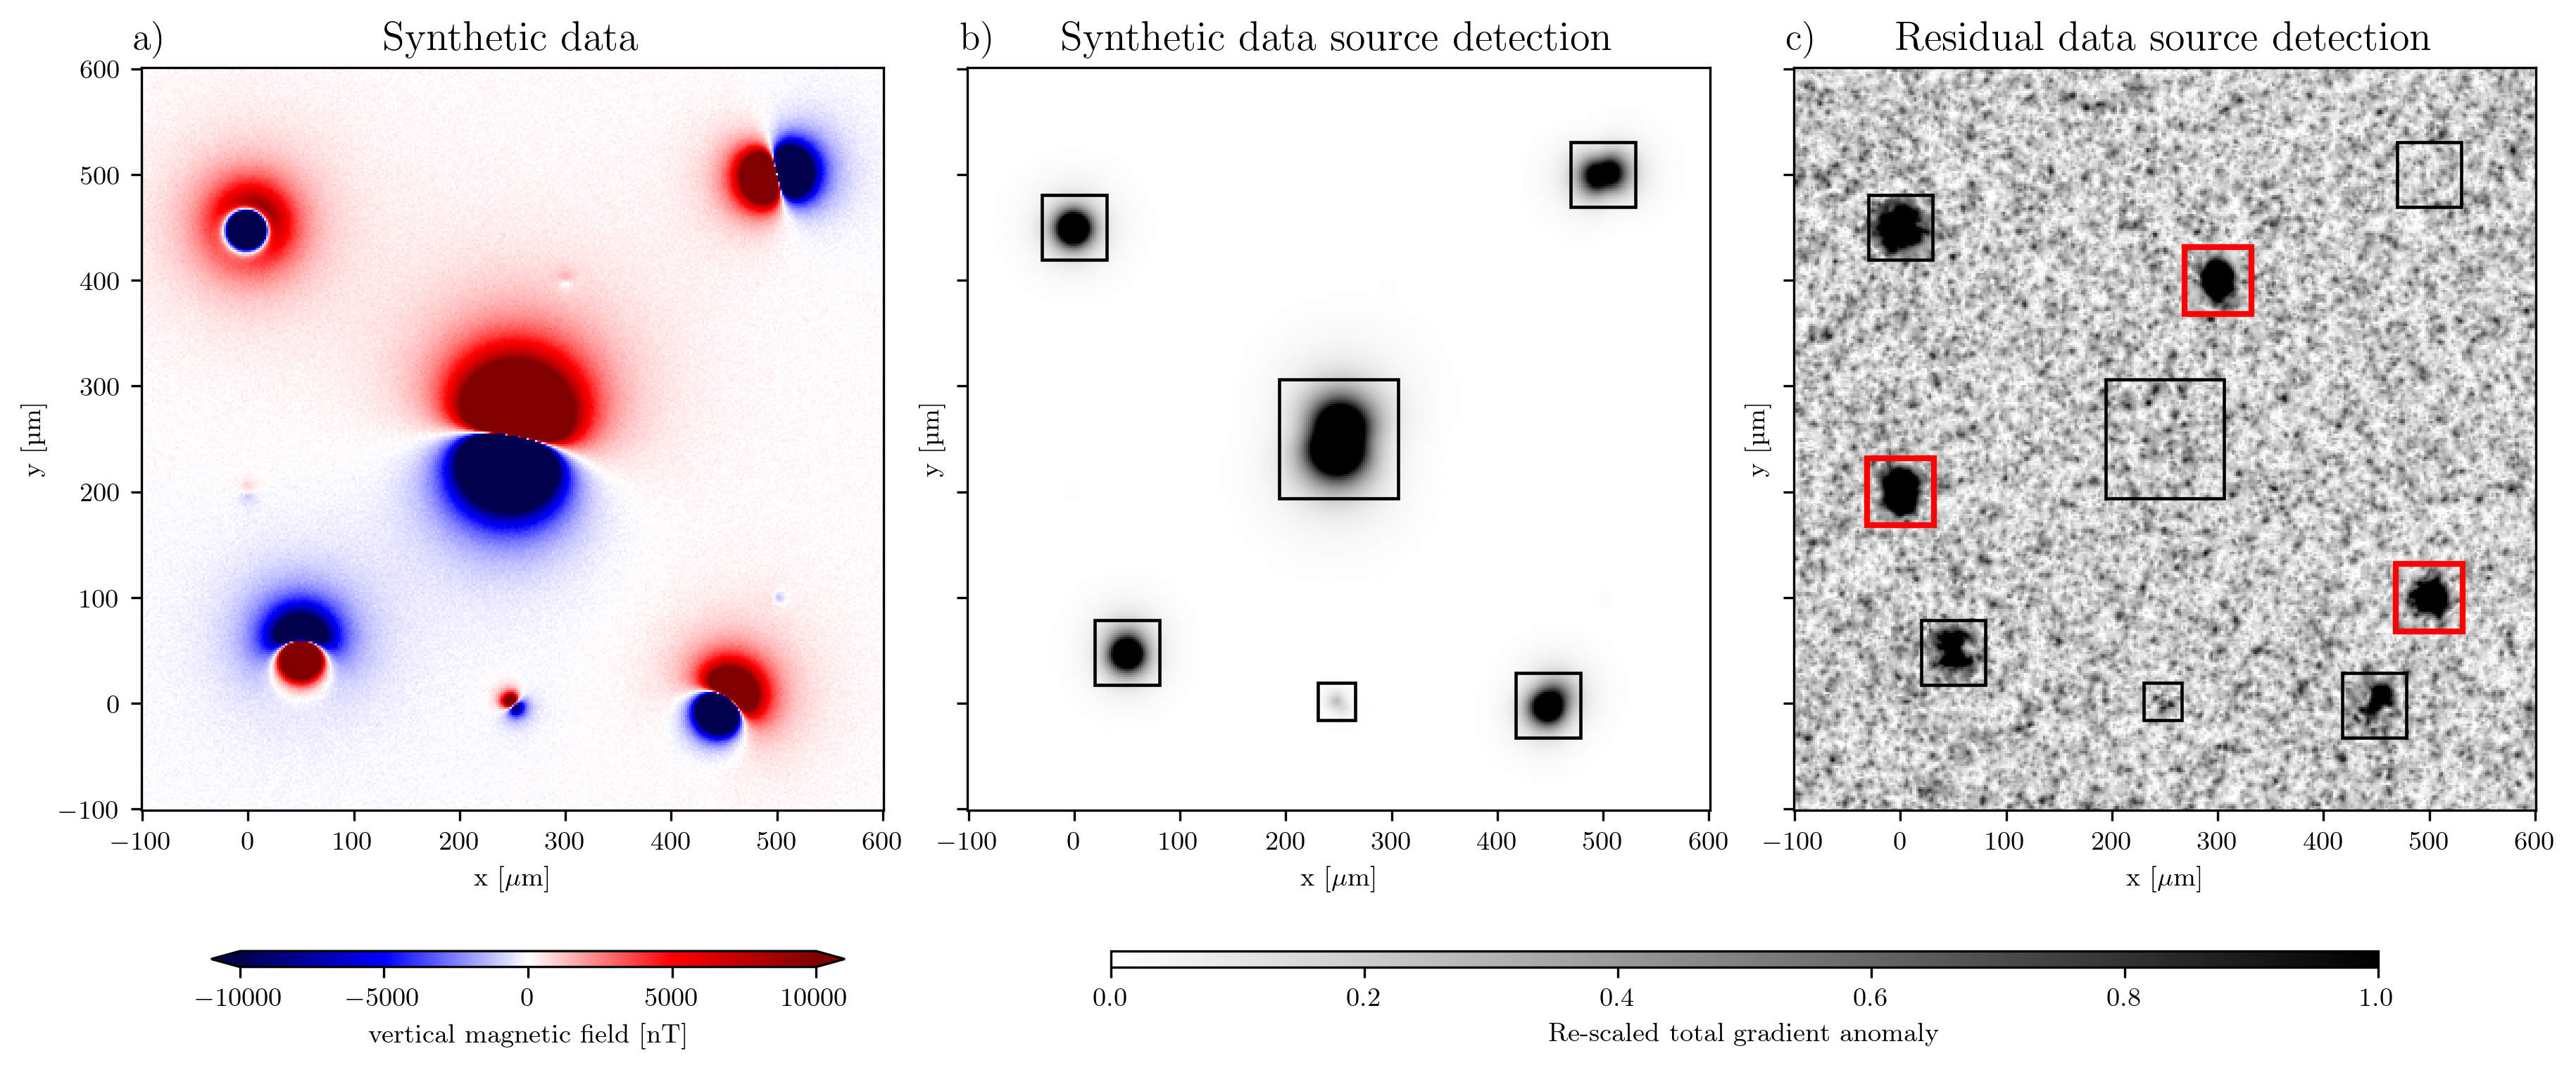
\includegraphics[width=1\linewidth]{micromag-interfering-sources/figures/re-detection-methodology.png}
      \caption{Source detection workflow on the residual anomaly. a) Synthetic sample featuring a wide range of magnetic moment intensities. b) The Blob detection algorithm identify the sources by using the total gradient obtained with the vertical component of the magnetic field. c) Result of the blob detection algorithm when applied to the total gradient of the residual anomaly.}
      \label{method-redetection}
    \end{figure}

%%%%%%%%%%%%%%%%%%%%%%%%%%%%%%%%%%%%%%%%%%%%%%%%%%%%%%%%%%%%%%%%%%%%%%
\section{Numerical simulations}

In this section, we evaluate the effectiveness of the interfering sources method, in comparison with the method proposed by \citet{Souza-Junior2024}, by applying it to two synthetic datasets. The tests are structured as follows:

\begin{enumerate}
    \item \textbf{Evaluating overlapping signal detection:} This test simulates a single map containing both strong and weak sources to evaluate the the new methodology's effectiveness in discerning and accurately locating the weaker sources, despite the interferences causing by the stronger ones.

    \item \textbf{Assessing performance with variable particle density:} This test introduces a more complex scenario by simulating a specific magnetization direction for the magnetic sources. Additionally, three different particle density scenarios are modeled to test whether the method can reliably recover the magnetization direction across all cases.

\end{enumerate}

\subsection{Evaluating overlapping signal detection}
\label{sec:synthetic-overlapping}

The first model scenario consists of several dipole sources with varying moment magnitudes, inclinations, and declinations, organized into three distinct groups. The first group contains 150 dipoles with random orientations and moment magnitudes an order of magnitude larger than those in the second group. The second group comprises 50 dipoles with a stable orientation: an inclination of \(\ang{35}\) (\(\pm \ang{5}\)), a declination of \(\ang{340}\) (\(\pm \ang{5}\)), and dipole moment magnitudes centered at \(1.0 \times 10^{-16} Am^2\). Additionally, a third group includes 9 sporadic, deeper, and strongly magnetized sources with random orientations and significantly higher dipole moments of \(1.0 \times 10^{-11} Am^2\). Which totals 209 magnetic particles.

To evaluate the methodologies, we simulate these magnetic sources randomly distributed within a synthetic thin with a field of view section measuring \(\qty{2000}{\micro\meter} \times \qty{2000}{\micro\meter}\). The synthetic vertical magnetic field data (\(b_z\)) are generated on a regular grid with \(\qty{2}{\micro\meter}\) spacing and a sensor sample distance of \(\qty{5}{\micro\meter}\), without any external applied field. Thus, the magnetic anomaly is solely caused by their dipole moment. High-frequency (\(\qty{50}{\nano\tesla}\) following \citet{Glenn2017}), spatially correlated pseudo-random noise, modeled after the spectral characteristics of the blank 2070615-NID08 diamond map, was added to replicate typical experimental conditions of other diamonds, providing a realistic approximation of a QDM measurement. The modeled sources were positioned at depths ranging from 1 to \(\qty{20}{\micro\meter}\). To further emulate actual acquisition conditions, a positive baseline shift of \(\qty{400}{\nano\tesla}\) \citep[following][]{Hess2024} is applied to the magnetic field data. This setup tests the algorithm's robustness and accuracy when handling systematically shifted and noise-corrupted magnetic field measurements, as commonly observed in magnetic microscopy experiments.

The synthetic data inversion was resolved using both the standard method \citep{Souza-Junior2024} and the newly proposed interfering sources methodology. A summary comparison of the classic Euler method and the iterative approach showed significant results in analyzing the synthetic data. The iterative Euler deconvolution method notably enhanced source detectability, with newly identified windows highlighted (green squares, Figure \ref{euler2}a). Figure \ref{euler2}b displays the 112 sources initially detected from the 209 modeled. Meanwhile, Figure \ref{euler2}c indicates that the iterative Euler method retrieved 166 sources. Initially, it may appear that the improvements of the iterative method  over the standard one in terms of tridimensional source location precision were modest. Yet, most previously identified sources demonstrate reduced position misfit (barring sporadic deeper ones). The larger misfits in Figure \ref{euler2}c are linked to the newly identified grains (represented by the colored squares), as their smaller dipole moment results in greater error in the Euler estimation. This increase in accuracy is crucial, especially in scenarios where stronger magnetic sources can distort the magnetic field anomaly of weaker sources. Although this new methodology can markedly increase the accuracy in the estimated position for virtually all sources, the biggest errors are still related to clustered sources. Also, in both cases, the Euler deconvolution seems unaffected by the presence of a shift in the magnetic field.


\begin{figure}[tb!]
  \centering
  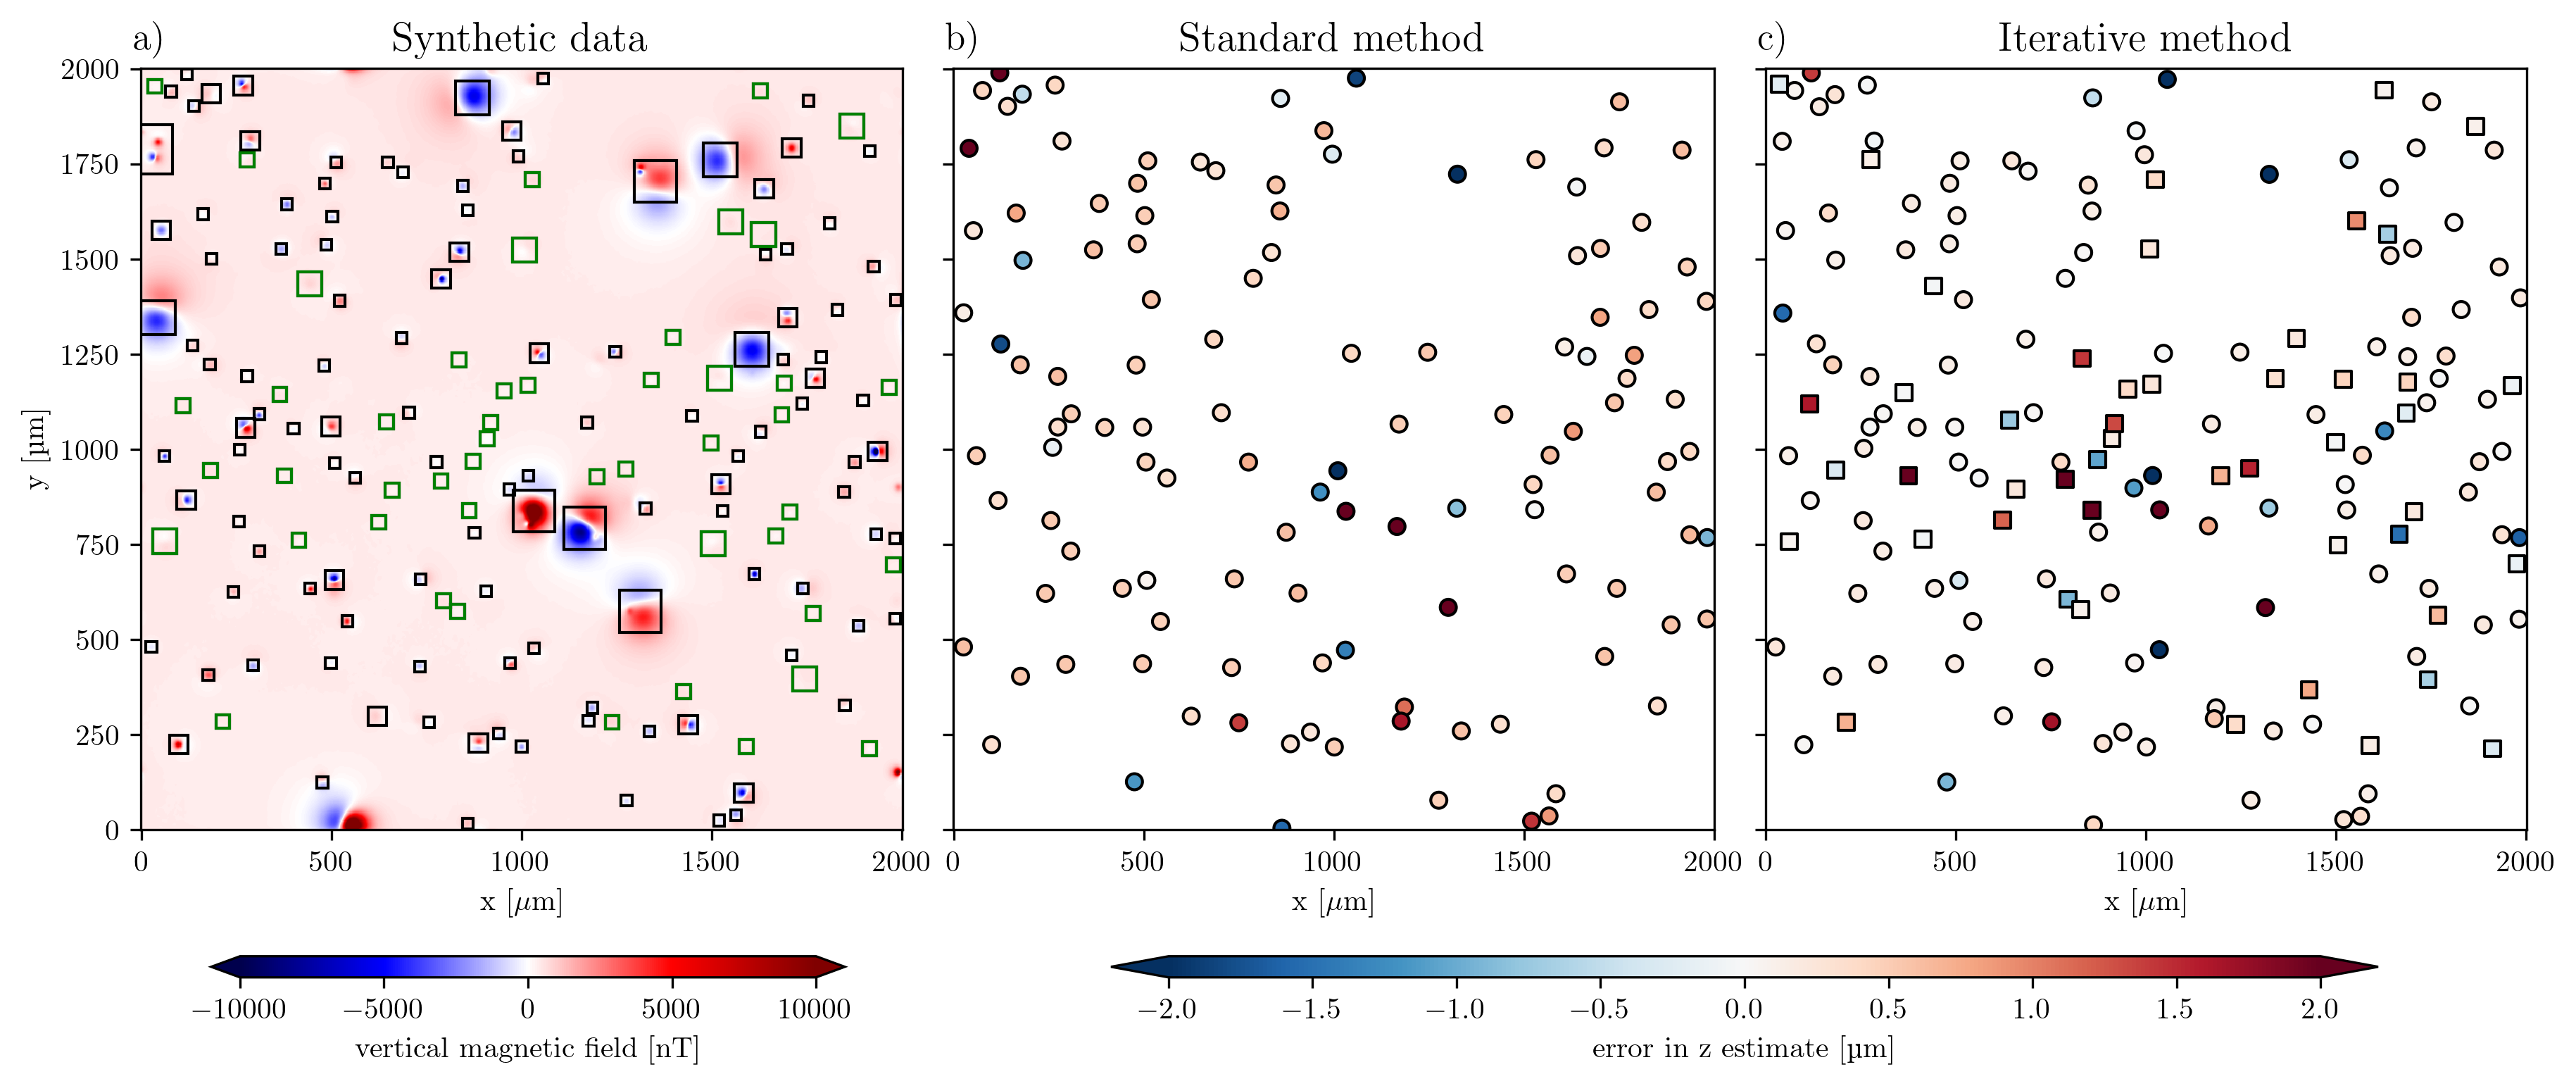
\includegraphics[width=1\linewidth]{micromag-interfering-sources/figures/euler-comparion-synthetic.png}
  \caption{
    Position estimation for the overlapping signals synthetic sample. (a) Initial detection window data for each magnetic source (black squares) and re-detection provided by the iterative solution (green squares). These data windows were used for the 3D position estimation of magnetic sources (colored circles) in the standard (b) and iterative (c) methodologies. Newly detected sources in the iterative method are represented as colored squares in panel (c).
  }
  \label{euler2}
\end{figure}

The iterative Euler estimated positions were used in the iterative magnetic inversion due to their superior accuracy. In contrast, the standard method relied on positions obtained from the original, unmodified algorithm. Figure~\ref{inversion2} presents a comparison of the estimated magnetic moment directions for the standard (Figure~\ref{inversion2}b) and iterative (Figure~\ref{inversion2}c) methods, in relation to the true directions (Figure~\ref{inversion2}a). As expected, the iterative method provides a better overall agreement with the true directions, recovering a larger number of sources with reliable estimates. The improvement is particularly noticeable as the iterative approach is capable of identifying signals from weaker particles, increasing the number of recovered sources. This has the potential to improve the statistical robustness of the estimated directions, making the method particularly useful for applications in magnetic microscopy.


\begin{figure}[tb!]
  \centering
  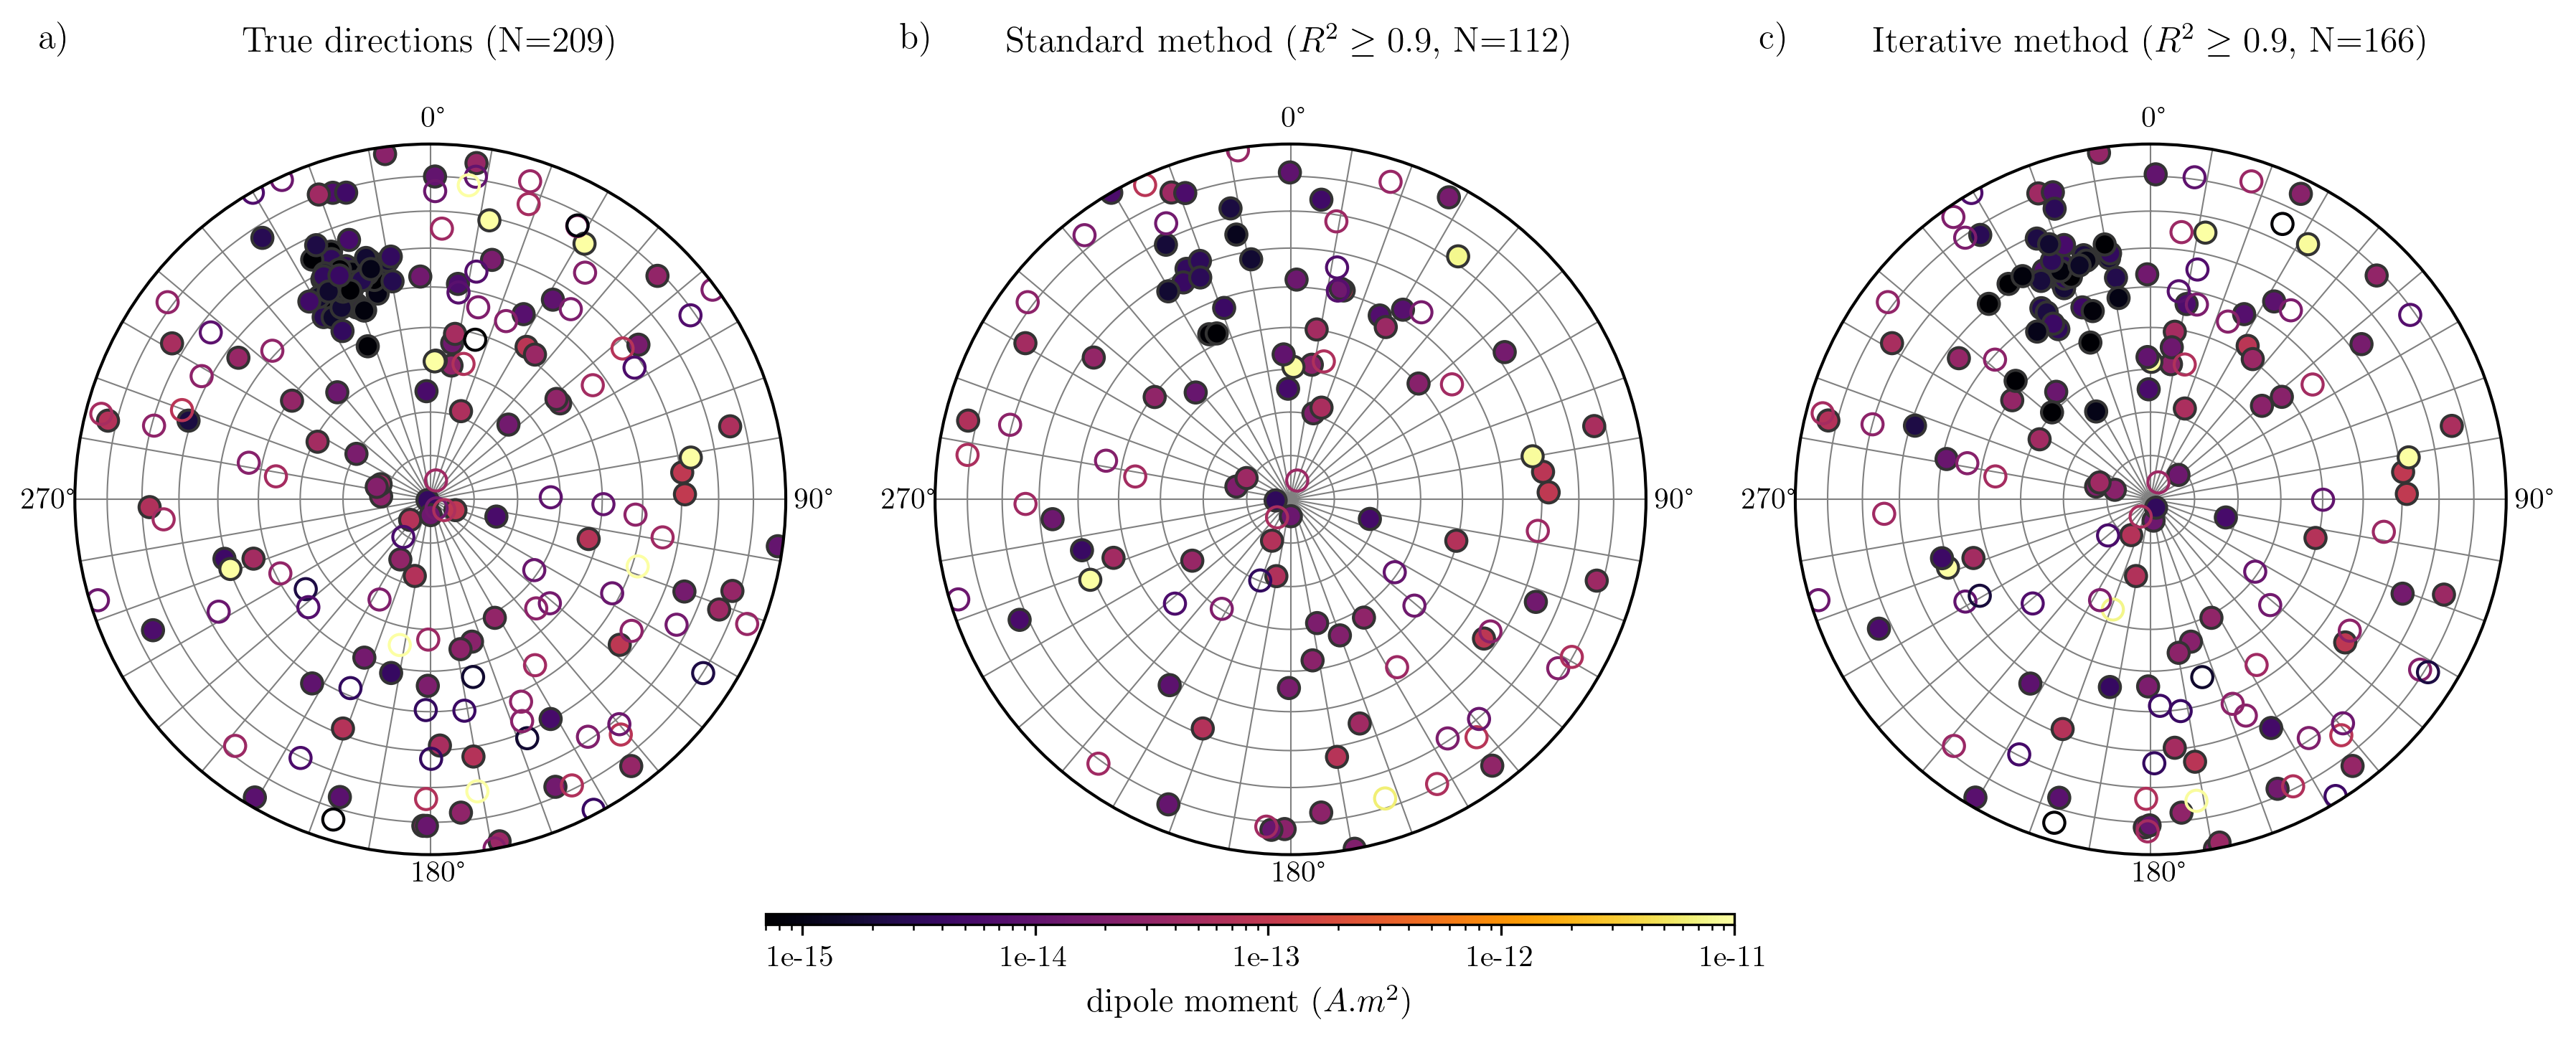
\includegraphics[width=1\linewidth]{micromag-interfering-sources/figures/synthetic-data-stereograms-comparison.png}
  \caption{
    Comparison of true and estimated dipole magnetic moments and directions for the overlapping signals in the synthetic sample. Panel (a) shows the true modeled direction, while panels (b) and (c) display the estimated vector directions obtained using the standard ($M = 112$) and iterative ($M = 166$) methods, respectively. Results for both methods were filtered based on the coefficient of determination ($R^2 \geq 0.9$). Directions are hued by magnitude of their magnetic moments. Open/closed circles indicate positive/negative inclinations.
  }
  \label{inversion2}
\end{figure}



\subsection{Assessing performance with variable particle density}

To evaluate the influence of particle density on the simulation results, we considered three different grain distributions with \(N = 500\) and \(N = 2500\), corresponding to grain densities of approximately \(9000\) and \(45000\,\mathrm{grains/mm^3}\), respectively. Examples of these distributions are shown in Figures~\ref{synthetic-data-maps}a,b. These densities were chosen to numerically simulate the concentrations expected in different rock types. Lower densities are typical of rocks with scarce magnetic grains, such as carbonates, while the highest density approximates rocks with higher particle concentrations, such as basalts.

\begin{figure}[tb!]
  \centering
  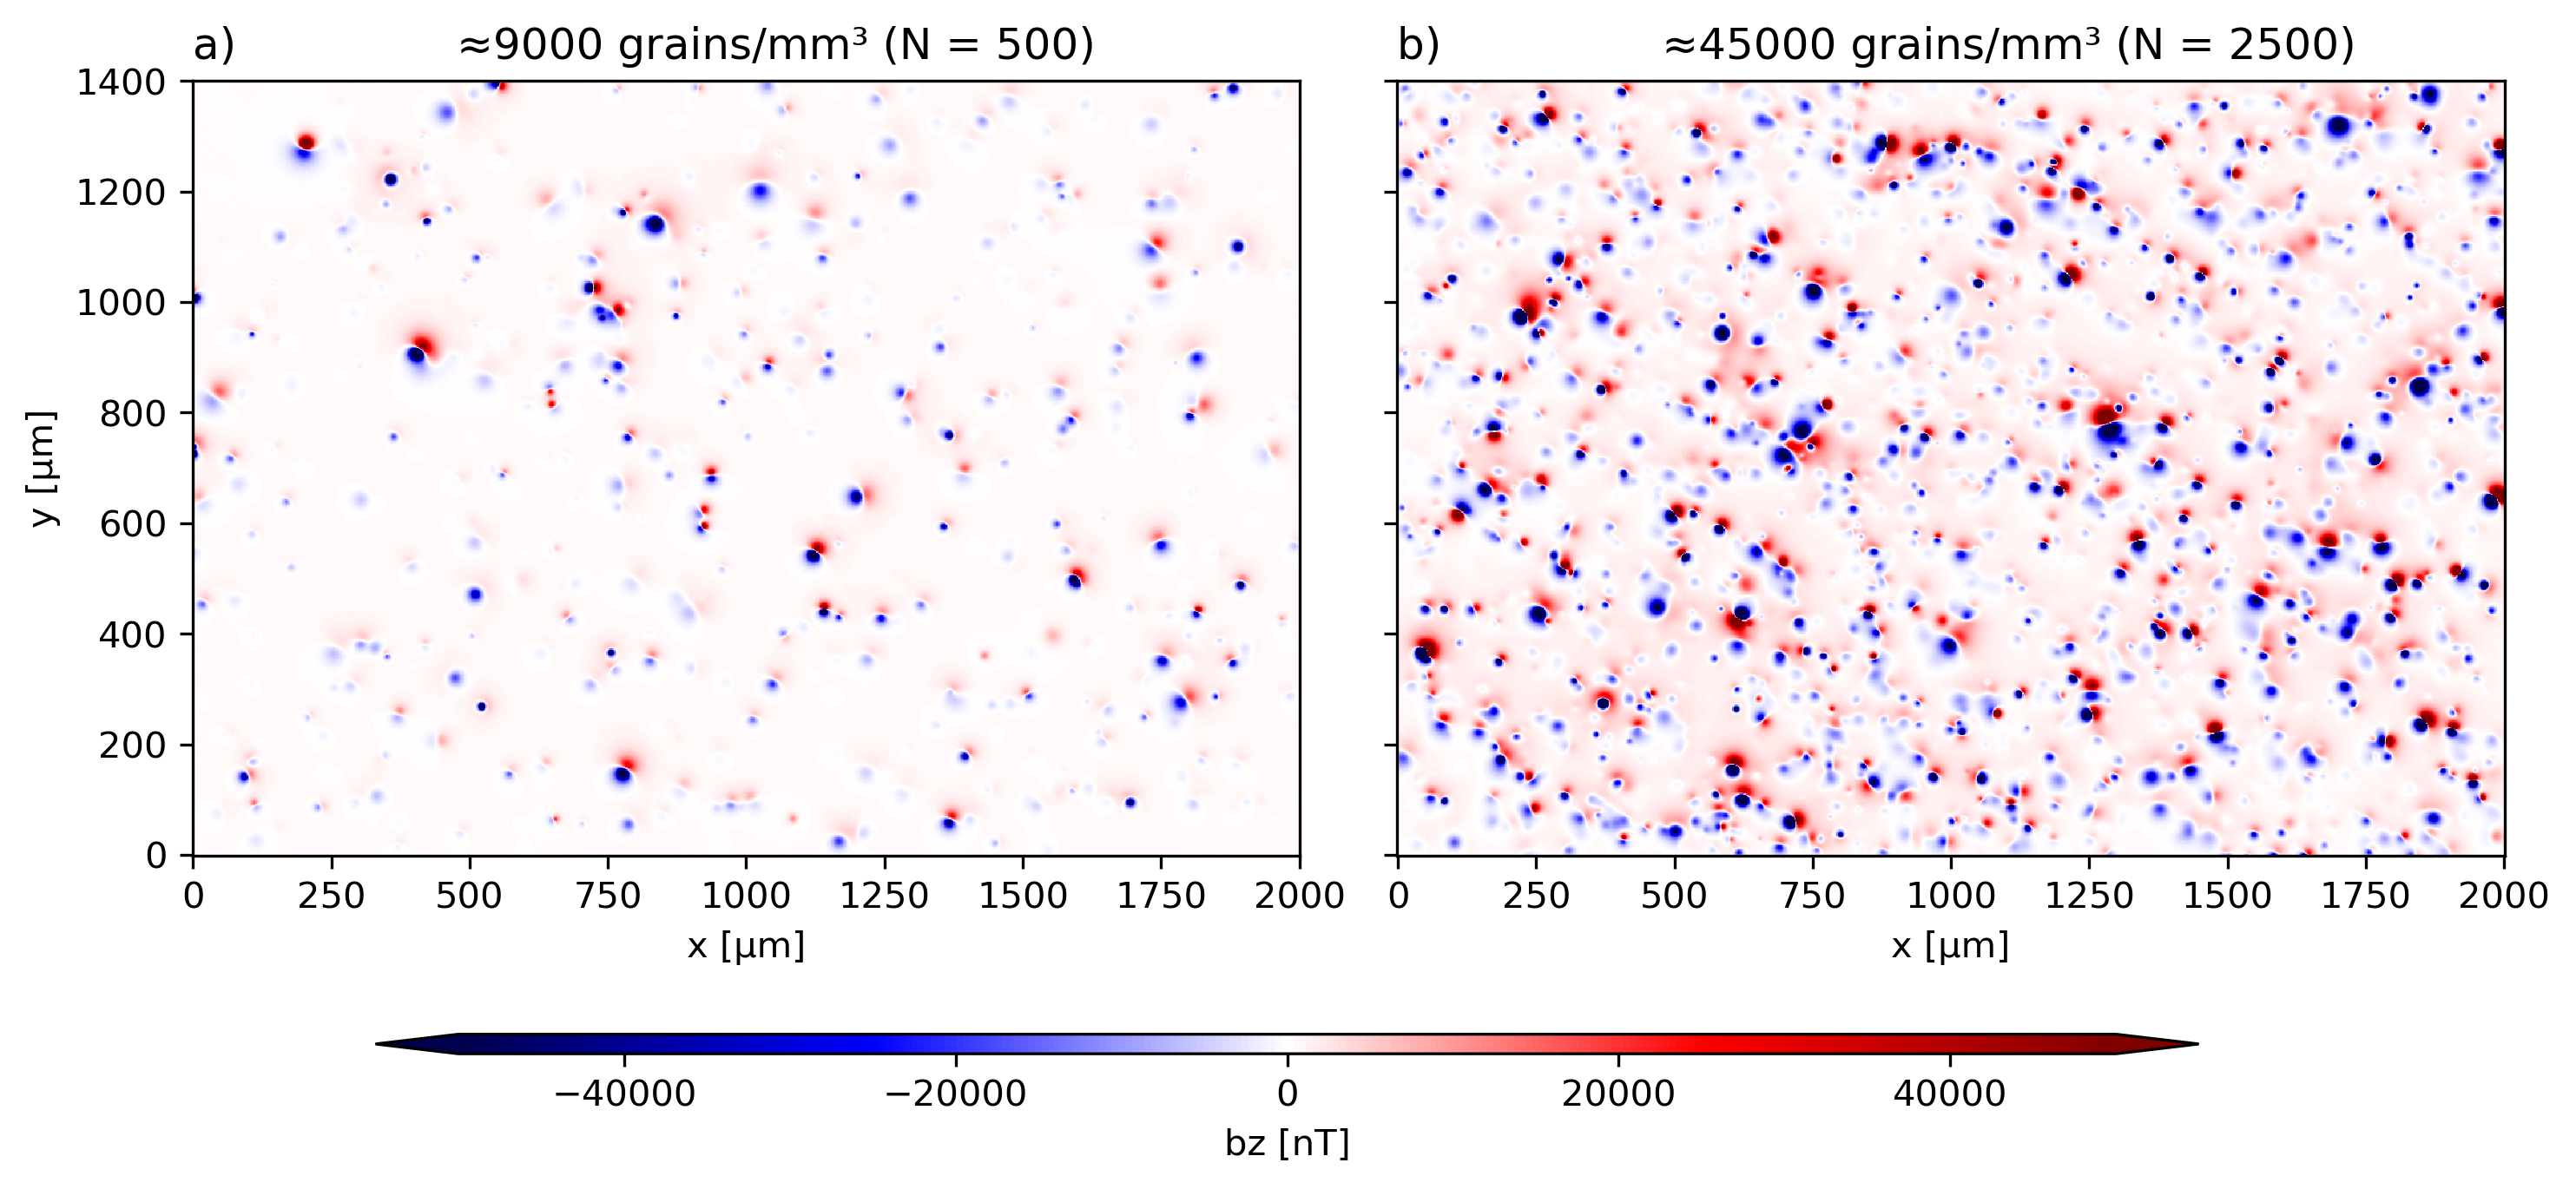
\includegraphics[width=1.0\linewidth]{micromag-interfering-sources/figures/synthetic-different-densities-maps.png}
  \caption{
Vertical component (\(b_z\)) magnetic data from synthetic grain distributions used to evaluate the influence of particle density on the simulation. Panel (a) shows an example with \(N = 500\), highlighting a low-density distribution of grains. Panel (b) illustrates the distribution for \(N = 1000\), presenting a moderate density of grains. Panel (c) displays the distribution for \(N = 2500\), showing a high-density grain arrangement.
  }
  \label{synthetic-data-maps}
\end{figure}


The directional parameters and magnetic moment intensities distributions were kept constant across all simulations, as the goal was to isolate the effects of increasing particle density. For each simulation, the total \(N\) magnetic dipole sources were created and randomly distributed across a thin section of \qty{2000}{\um} \(\times\) \qty{1400}{\um}. The dipole moments were sampled from a lognormal distribution centered at a mean amplitude of \(1 \times 10^{-14}\,\mathrm{A \cdot m^2}\), with a standard deviation spanning two orders of magnitude. This configuration ensures that most of the distribution is concentrated around the mean, while also allowing for the presence of particles with magnetic moments as strong as \(10^{-11}\,\mathrm{A \cdot m^2}\), simulating larger particles with a greater influence on the magnetic field compared to weaker particles. The modeled sources were also positioned at pseudo-random depths ranging from 1 to \(\qty{20}{\micro\meter}\).

A variety of geological processes can lead to the acquisition of natural remanent magnetization (NRM). If the NRM is primary—acquired at the same time as the rock—it will generally align with the ambient magnetic field, such as a planetary field. However, the alignment of individual grains is influenced by multiple factors, including particle properties \citep[shape, size, domain state,][]{Bellon2025} and the conditions under which NRM is acquired, such as the cooling rate of lavas. As a result, while individual grain signals may show a general tendency toward alignment, the magnetic moments of many particles will still exhibit some degree of random orientation. However, modeling TRM directions is not a straight-forward task, instead we can mirror an isothermal remanent magnetization (IRM) behavior in our synthetic data. Thus by setting the inclination and declination of directional parameters primarily at 30° and 330°, respectively, and 50° dispersion angle introduced variability within spherical statistics, where directional data extends over a unit sphere rather than Cartesian coordinates. This angle indicates a broad spread of directions around the mean, accounting for significant variability in dipole directions, which is crucial for accurately representing the natural diversity of magnetic sources.

The synthetic magnetic field \(b_z\) was computed over a grid with a \qty{2}{\um} spacing, and the measurement plane was set at a constant height of \qty{5}{\um} above the thin section. The same high-frequency QDM spatially correlated pseudo-random noise was added to the computed field to mimic realistic measurement conditions. Additionally, a positive baseline shift of \(\qty{400}{\nano\tesla}\) \citep[following][]{Hess2024} was introduced to replicate the acquisition process in magnetic microscopy. The simulations were conducted in a zero external field environment, where all signals generated in the maps were solely and exclusively caused by the magnetization of the simulated particles, simulating real acquisitions typically performed in magnetically shielded rooms to eliminate the influence of the Earth's geomagnetic field. A total of 10 simulations were carried out for each different particle density level.

The results reveal a clear difference in the performance of the standard (red curves and left stereoplots) and iterative (blue curves and right stereoplots) methods in reconstructing the synthetic IRM direction imparted in the simulations. As shown in Figure~\ref{synthetic-data-stereograms}a, for lower densities of particles, both methods perform almost the same, given that in this case, the amount of interference between the sources is small. This is also observed for the mid-term density (Figure~\ref{synthetic-data-stereograms}b). However, for the higher density of magnetic particles (Figure~\ref{synthetic-data-stereograms}c), the iterative method starts to outperform the standard method. This shows the superiority of the iterative technique, as there are no randomly stronger particles simulating different viscous directions. Even though there are many strong sources, they all follow the same distribution around the synthetic direction, similar to what happens in an IRM induced sample. This could explain, alongside the low density of particles, the good results presented by the real carbonatic data presented by \citet{Souza-Junior2024}, which was subjected to strong IRM, though it remains ambiguous whether the results are due to the low particle density or the IRM. For this reason, the next tests involved samples with natural remanent magnetization.

\begin{figure}[tb!]
  \centering
  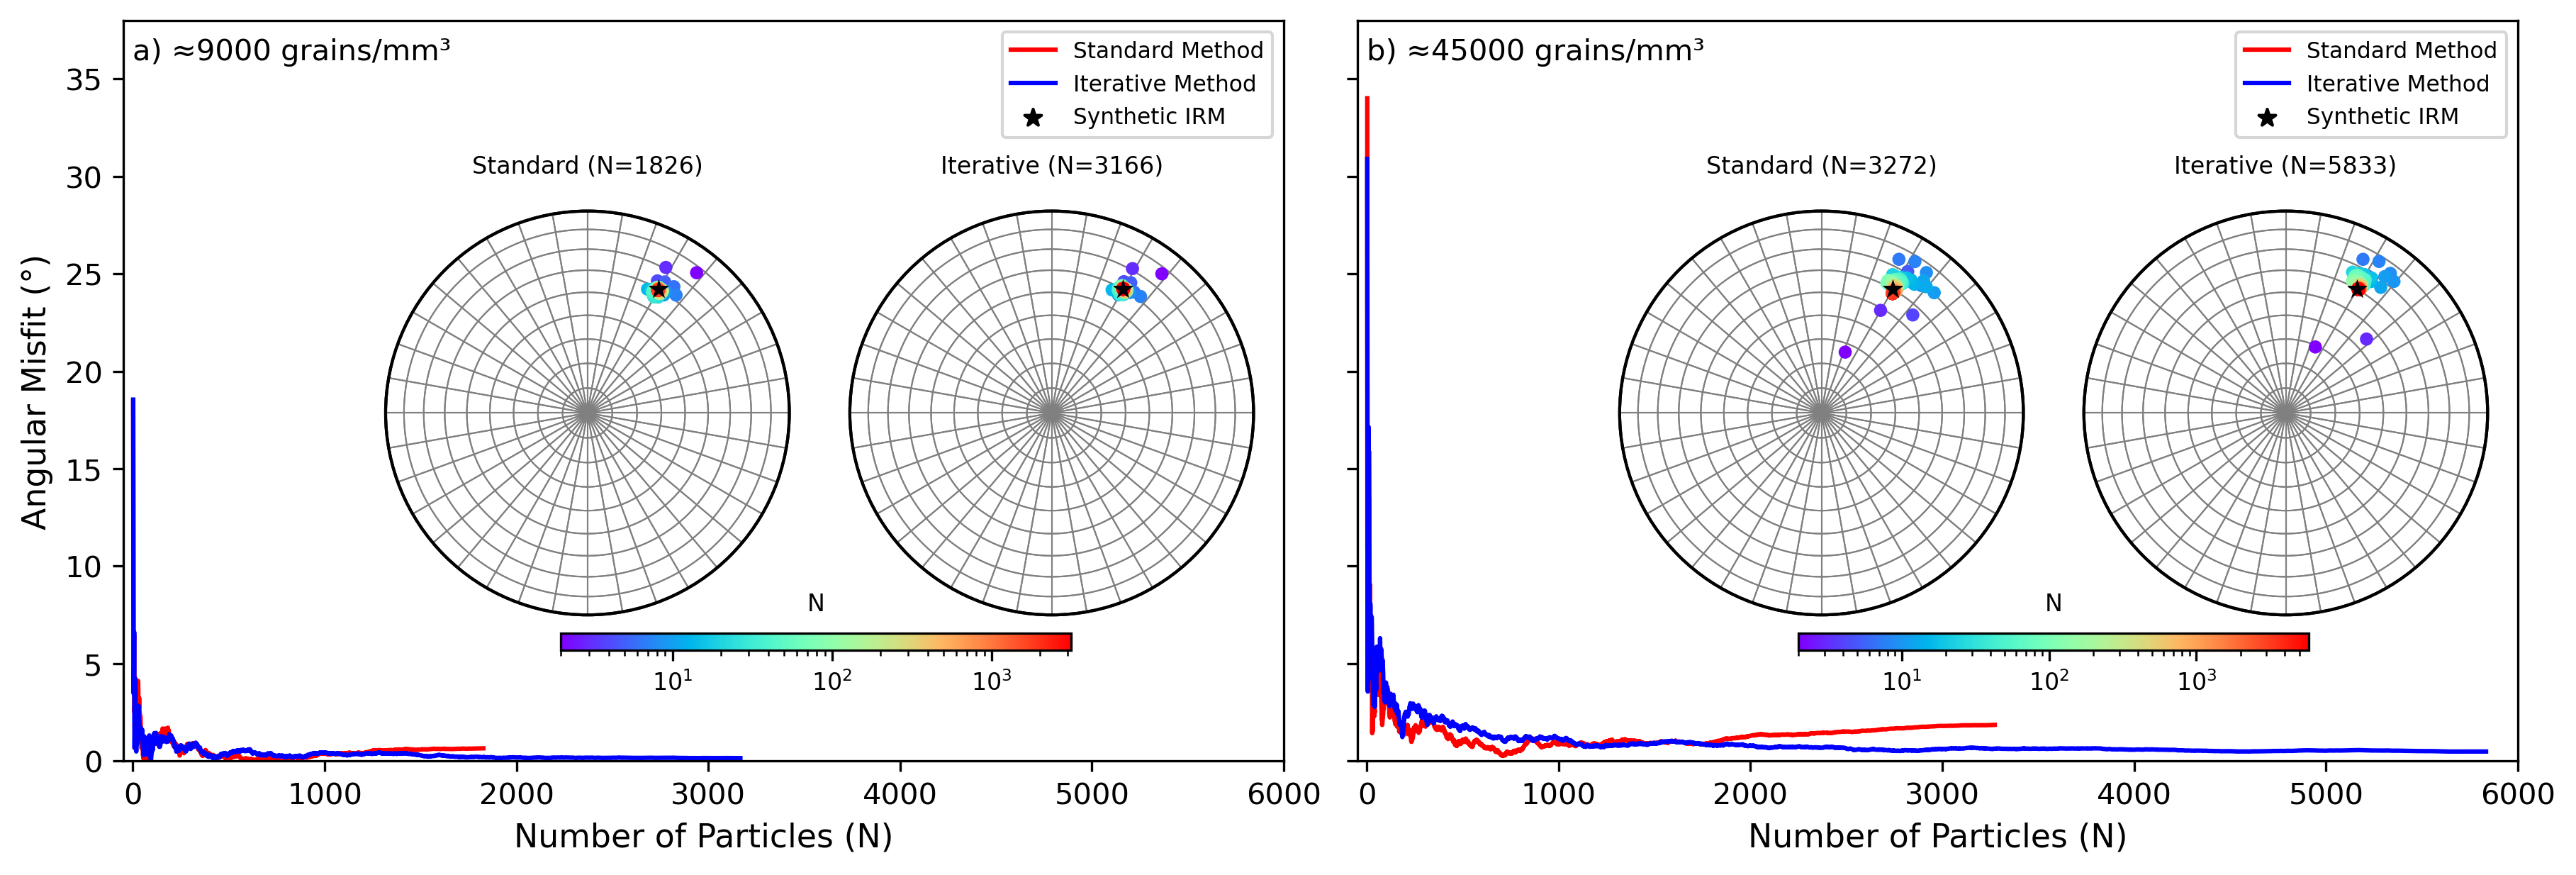
\includegraphics[width=1.0\linewidth]{micromag-interfering-sources/figures/synthetic-different-densities-stereoplot.png}
  \caption{
Comparison of the magnetic directions obtained using the original (red line and left stereogram) and the iterative (blue line and right stereogram) methods on each synthetic grain distributions simulation. Panel (a) shows the angular misfit between the cumulative vector and the measured magnetic direction for the low-density distribution. Panel (b) illustrates the angular misfit for the moderate-density distribution. Finally, panel (c) presents the results for high-density distribution. The stereographic projections of the filtered magnetic vectors ($R^2 \geq 0.9$) for each density are also shown, with modeled bias direction (star) and the cumulative direction (square) indicated. The color gradient represents the logarithmic scale of particle counts, with warmer colors indicating higher particle concentrations.
  }
  \label{synthetic-data-stereograms}
\end{figure}


\section{Real data applications}

After demonstrating the applicability of the new methodology through the numerical simulations, we applied it to real MM data. The magnetic particles \citep[most commonly magnetite,][]{OReilly1984} acquire TRM as they cool below their Curie temperature, with the magnetization direction becoming "locked in" upon reaching the blocking temperature \citep{Dunlop1997}. When grains are sufficiently small and exhibit homogeneous, unidirectional magnetization (single domain, SD), the acquisition and preservation of magnetic signals are physically described by Néel’s theory \citep{Neel1949, Neel1955}. This allows them to retain remanent magnetization for billions of years, making them excellent recorders of the paleomagnetic field. In addition to SD particles, pseudo-single domain (PSD) particles—characterized by flower and vortex states—are also stable and can preserve magnetization for timescales comparable to the age of the Solar System \citep{Nagy2017, Lascu2018,Bellon-2024a}. Conversely, Néel’s theory does not apply to larger particles (multidomain, MD), which have unstable remanent magnetization \citep[e.g., due to viscous domain reorganization,][]{DeGroot2014}, limiting their capacity to reliably record the geomagnetic field.

In this section, we worked with two distinct samples. The NRM of these samples was measured using the 2G RAPID Superconducting Rock Magnetometer at the Harvard Paleomagnetics Lab, Department of Earth and Planetary Sciences, Harvard University. As a result, the measurements encompass both the primary TRM and any possible viscous components acquired through the natural magnetic relaxation of some particles. Additionally, to ensure consistency between the magnetometer measurements, which were taken vertically, and the maps produced with the QDM, it was necessary to apply a 90-degree clockwise rotation around the \textit{x}-axis to the vertical measurements. This rotation ensures that both measurements are in the same reference frame.

The samples we used provide test to:

\begin{enumerate}
\item \textbf{Evaluate a stable, dispersed assembly:} The first test focuses on the analysis of a thin section made of an archaeological ceramic (Figure~\ref{real-data-maps}a). This sample is characterized by a moderate density of magnetic particles, most falling into SD and PSD categories. The goal of this test is to assess the method’s performance in real samples where the magnetic carriers are stable, and the influence of unstable domains is minimal. This setting allows for a clear evaluation of the methodology’s sensitivity and accuracy when working with well-defined magnetic signals.

\item \textbf{Evaluate a Complex Densely Packed Assembly:} The second test involves the examination of the basaltic rock sample (Figure~\ref{real-data-maps}b). This sample acquired its TRM during the natural cooling of mafic lava, leading to a high density of magnetic particles. Unlike the ceramic sample, the basalt is significantly influenced by unstable MD particles, which introduce additional complexity to the magnetic signal. The aim of this test is to verify the method’s effectiveness in identifying and analyzing magnetic sources in challenging conditions, where densely packed magnetic carriers and the presence of unstable remanent magnetization could affect the reliability of the results. This is a more complex and challenging scenario, providing a test for the accuracy of the method to identify and interpret magnetic sources in samples with densely packed and less stable magnetic carriers.
\end{enumerate}

\begin{figure}[tb!]
  \centering
  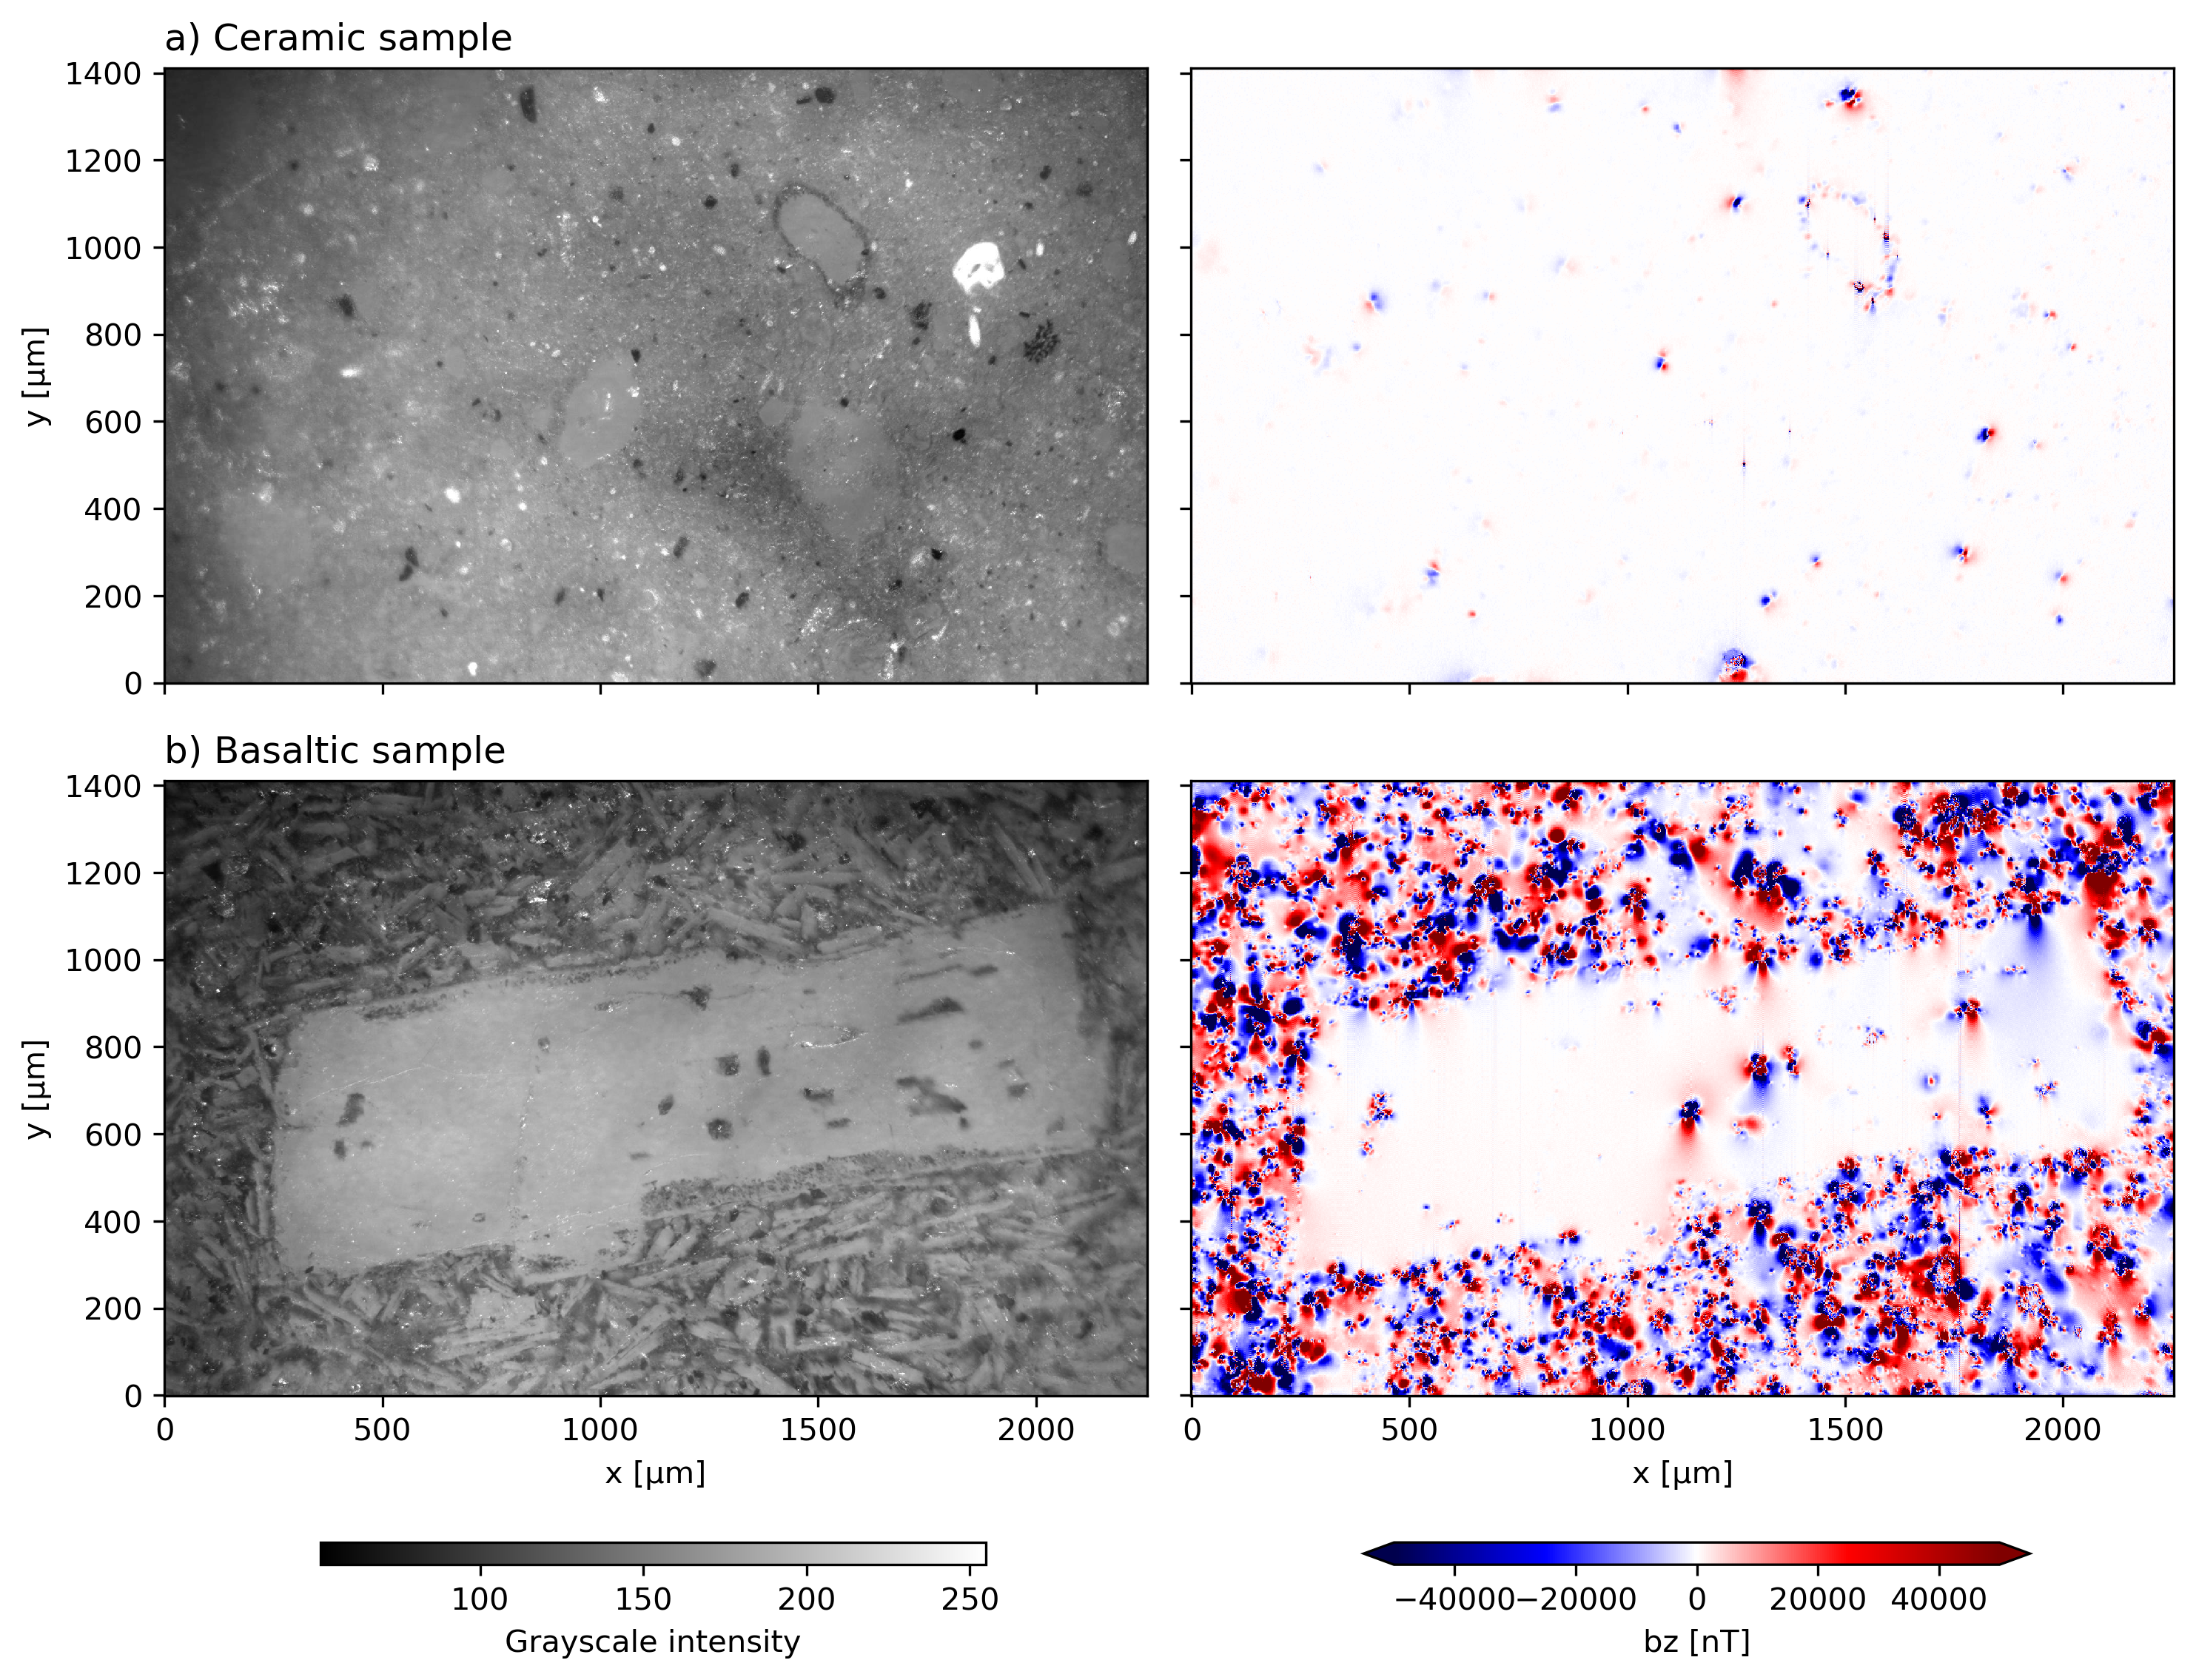
\includegraphics[width=1\linewidth]{micromag-interfering-sources/figures/real-data-maps.png}
  \caption{
   LED picture (left) and vertical component (\(b_z\), right) magnetic data from real samples observed at \(z = 5\) µm. Panel (a) shows an example from the ceramic tile sample, highlighting its key characteristics, including the presence of isolated dipolar particle signals and clusters related to larger particles. Panel (b) presents an example from the basaltic sample, displaying two main occurrences of magnetic signals: the first is a high density of signals distributed within the matrix, and the second appears as inclusions in plagioclase phenocrysts.
  }
  \label{real-data-maps}
\end{figure}

\subsection{Evaluation with a stable, dispersed assembly}

To evaluate the feasibility of magnetic microscopy techniques in detecting and characterizing TRM, we selected a well-preserved fragment of baked clay pavement tile (sample RSLG1) from the archaeological site São Luiz Gonzaga reduction (1657-1687 AD). This fragment was studied by \citet{Poletti2016}. According to these authors, the magnetic properties of the sample indicate that magnetization is carried by a low-coercivity phase, most likely PSD Ti-poor titanomagnetite. Their interpretation is supported by the IRM curves saturated at fields up to approximately 0.3 T, narrow hysteresis loops, and maximum NRM demagnetization temperatures around 550°C. First order reversal curves (FORC) also confirm a predominance of non-interacting SD/PSD grains. These characteristics make the sample an ideal candidate for magnetic microscopy studies aimed at investigating its natural remanent magnetization.

We mapped the NRM of the thin-section sample using the QDM at the Harvard Paleomagnetics Lab, Department of Earth and Planetary Sciences, Harvard University. All QDM data were taken in projected magnetic microscopy (PMM) mode and converted to the vertical component of the magnetic field ($b_z$) using a spectral approach \citep{Fu2020, Glenn2017, Lima2009}. We applied a 0.9 mT bias magnetic field during measurement, which was reversed periodically to result in a net bias field of ~400 nT. A total of 20 randomly selected regions were subjected to this procedure to ensure representative coverage of the sample's magnetic properties, in which Figure~\ref{real-data-maps}a showcases one of the maps obtained. The scanned area measured $\qty{1410}{\um} \times \qty{2256}{\um}$ with a grid spacing of \qty{2.35}{\um} ($N = 576 \times 10^{3}$). Data acquisition was conducted at a constant sensor-sample distance of \qty{1} - \qty{5}{\um}. This allowed for high-resolution mapping of the magnetic field distribution.

We have applied both the standard and iterative algorithms to this data, and all magnetic vectors associated with the identified particles were compiled into a database. This dataset was filtered based on the model's coefficient of determination ($R^2$), with only vectors meeting the criterion of $R^2 \geq 0.9$ being retained. This filtering is important to remove inversion results that do not comply with our dipolar assumption. An $R^2 \geq 0.9$ means that the only results that closely fit the data are kept (the maximum value of $R^2$ is 1).  The selected vectors were then ordered by intensity and progressively summed. At each step, the cumulative vector was compared with the NRM measured of the whole sample (which was acquired with a 2G Superconducting Rock Magnetometer, see the Methodology section for more details).

The comparison between the standard and iterative algorithms highlights significant differences in their ability to reconstruct the NRM of the sample. As shown in Figure~\ref{ceramic-data-stereograms}, the angular misfit between the cumulative magnetic vector and the measured NRM decreases more effectively with the iterative approach. We further remove outliers in the dataset by excluding values that are 1.5 times larger than the third-quartile of the dipole moment intensities. While the non-filtered standard method results in a consistently higher misfit, stabilizing around \ang{55}, the iterative method quickly refines the alignment, reducing the misfit to approximately \ang{10} within a few hundred particles. While for filtered curves this misfit difference reduces, there are virtually no changes in the iterative method result. This indicates that the iterative approach is more efficient in capturing the true remanent magnetization with fewer contributing grains. The stereographic projections further support this observation by illustrating the directional distribution of the filtered vectors for each method, where the iterative approach yields a distribution more closely aligned with the measured NRM (star symbol) and the cumulative direction (square symbol). These results demonstrate that the iterative method significantly enhances the accuracy of NRM reconstruction by effectively mitigating directional dispersion.

The limited improvement threshold in directional accuracy, even as more particles are added, is a noteworthy observation. We propose two possible contributing factors. First, as previously discussed, the bias of individual particles towards the magnetic field is only at the level of $\sim1\%$. When measuring the total NRM at the macroscopic scale, the contributions of all grains are summed, allowing randomly oriented signals to cancel out while the more aligned grains enhance the overall alignment with the field direction. Classical rock thin sections, like the one used in this study, are typically prepared at a thickness of around \qty{30}{\um} to facilitate the identification of mineral features under a petrographic microscope. Within such a thin section, millions of magnetic minerals are likely present. However, in MM data acquisition, we only sample a small portion of the entire thin section. Even within this measured area, not all magnetic signals are fully detected, as the measured magnetic moment depends on both the depth of the particles and their magnetic strength. As a result, when more particle directions are incorporated into the combined magnetic signal, a saturation effect may occur. Beyond a certain threshold, the inclusion of additional, randomly oriented signals could outweigh the contribution of well-aligned grains, limiting further improvement in directional accuracy. This would explain why, despite increasing the number of particles, the expected refinement in the reconstructed direction is not observed.

The second hypothesis involves human-induced errors during the measurement process. The sample had to be manually positioned and oriented in both the QDM and the 2G magnetometer, introducing potential sources of misalignment. In the 2G magnetometer, the sample was measured in a vertical orientation and later rotated to match the reference frame of the thin section used in the QDM analysis. This manual handling and reorientation may have introduced small but cumulative misalignments, contributing to the observed directional discrepancies. Another potential source of bias in the 2G magnetometer measurements could be contamination, either from the glass slide or another external source near the sample.

\begin{figure}[tb!]
  \centering
  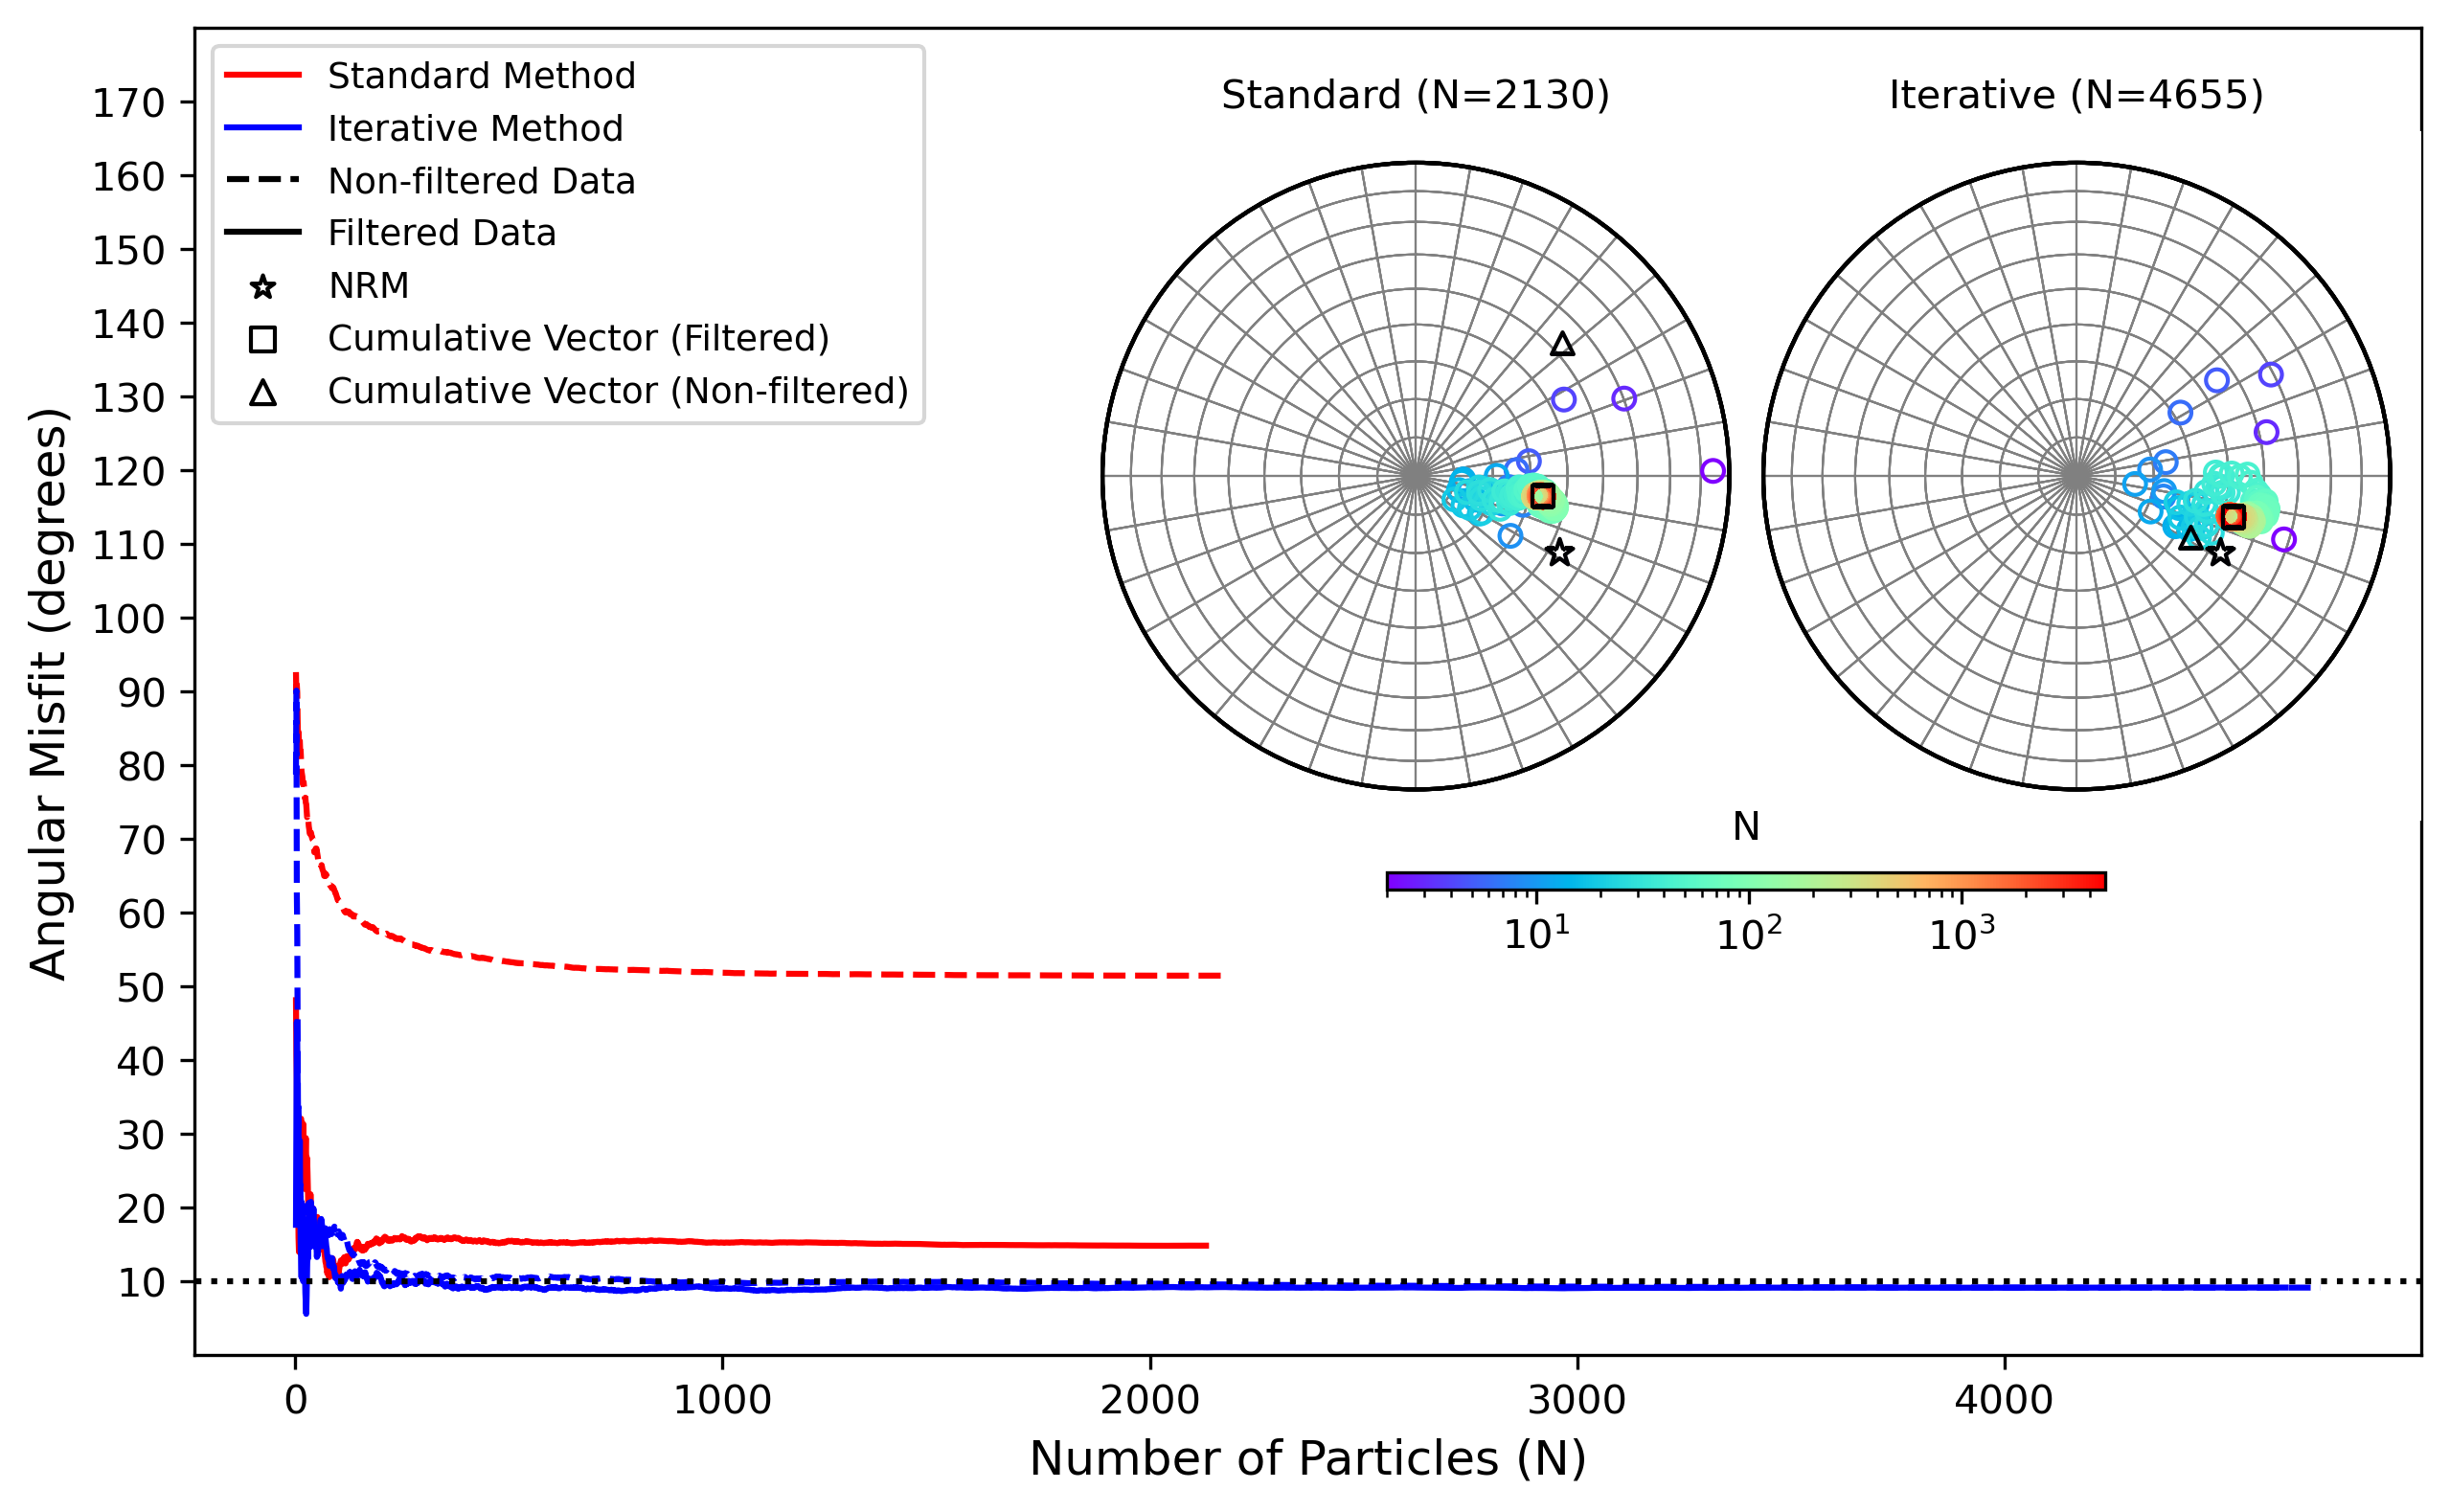
\includegraphics[width=1\linewidth]{micromag-interfering-sources/figures/ceramic-data-stereoplot.png}
  \caption{
  Comparison of the standard (red) and iterative (blue) algorithms in reconstructing the NRM direction from the ceramic sample. (Left) Angular misfit between the cumulative vector and the measured NRM as a function of the number of particles ($N$). (Right) Stereographic projections of the filtered magnetic vectors ($R^2 \geq 0.9$) for both methods, with the measured NRM (star), non-filtered cumulative direction (triangle), and the filtered cumulative direction (square) indicated. The color gradient denotes the logarithmic scale of particle counts, with warmer colors representing higher concentrations. The solid-lined and dashed-lined curves represent the non-filtered and outliers filtered data, respectively.
  }
  \label{ceramic-data-stereograms}
\end{figure}

%%%%%%%%%%%%%%%%%%%%%%%%%%%%%%%%%%%%%%%%%%%%%%%%%%%%%%%%%%%%%%%%%%%%%%%%%%%%%%%
\subsection{Evaluation with a complex densely packed assembly}

In order to apply our method to a more magnetically complex sample, we have chosen a basalt from the Caviahue-Copahue volcanic complex (Argentina), specifically a core from the Cola de Zorro Formation (COP01) \citep{Moncinhatto2019}. This formation exhibits a flow-aligned fabric, marked by plagioclase crystals, but also contains both phenocrysts and smaller crystals in the matrix showing a trachytic texture. Its magnetic mineralogy is mainly composed of low-Ti magnetite, with most macroscopic crystal sizes ranging from 10 to 50 \si{\micro\meter} \citep{Moncinhatto2019}. This size distribution is reflected in the high-field experiments, including IRM acquisition curves, hysteresis loops, and FORC diagrams. They reveal saturation at fields around 0.2 \si{T}, coercivities below 10 \si{mT}, and the FORC diagrams are typical of multidomain (MD) grains. Nonetheless, other samples within the same formation display coercivities between 10 and 20 \si{mT} and FORC diagrams characteristic of magnetite with a PSD behavior, or mixtures of SD and MD grains.

The acquisition of QDM data was essentially the same as the aforementioned experiment with the ceramic tile. The QDM scans were performed to capture the magnetic field distribution at high spatial resolution. To better compare the results with the tile sample, the same number of randomized mapping spots was performed. Figure~\ref{real-data-maps}b shows one example of the maps obtained. The resulting data enabled the calculation of angular misfit as a function of the number of particles, providing insight into the reliability of different analytical methods.

The results reveal a clear difference in the performance of the standard and iterative methods in reconstructing the NRM direction. As shown in Figure~\ref{basalt-data-stereograms}, the iterative method consistently achieves lower angular misfit values, before and after the intensity filtering, as more particles are incorporated, demonstrating improved accuracy and stability. In contrast, while the standard method also reduces the misfit over time, especially after the filtering, it stabilizes around 5 degrees only after approximately a thousand grains. The stereographic projections further illustrate these differences. The standard method exhibits a wider spread of vectors, suggesting that many individual particle contributions remain misaligned. Meanwhile, the iterative method results in a more tightly clustered distribution, with the misfit tending toward zero as the number of particles increases (although there is also, seemingly, a stagnation threshold). This suggests that the iterative approach is more effective in refining the directional signal, leading to greater precision in the reconstructed magnetization.

\begin{figure}[tb!]
  \centering
  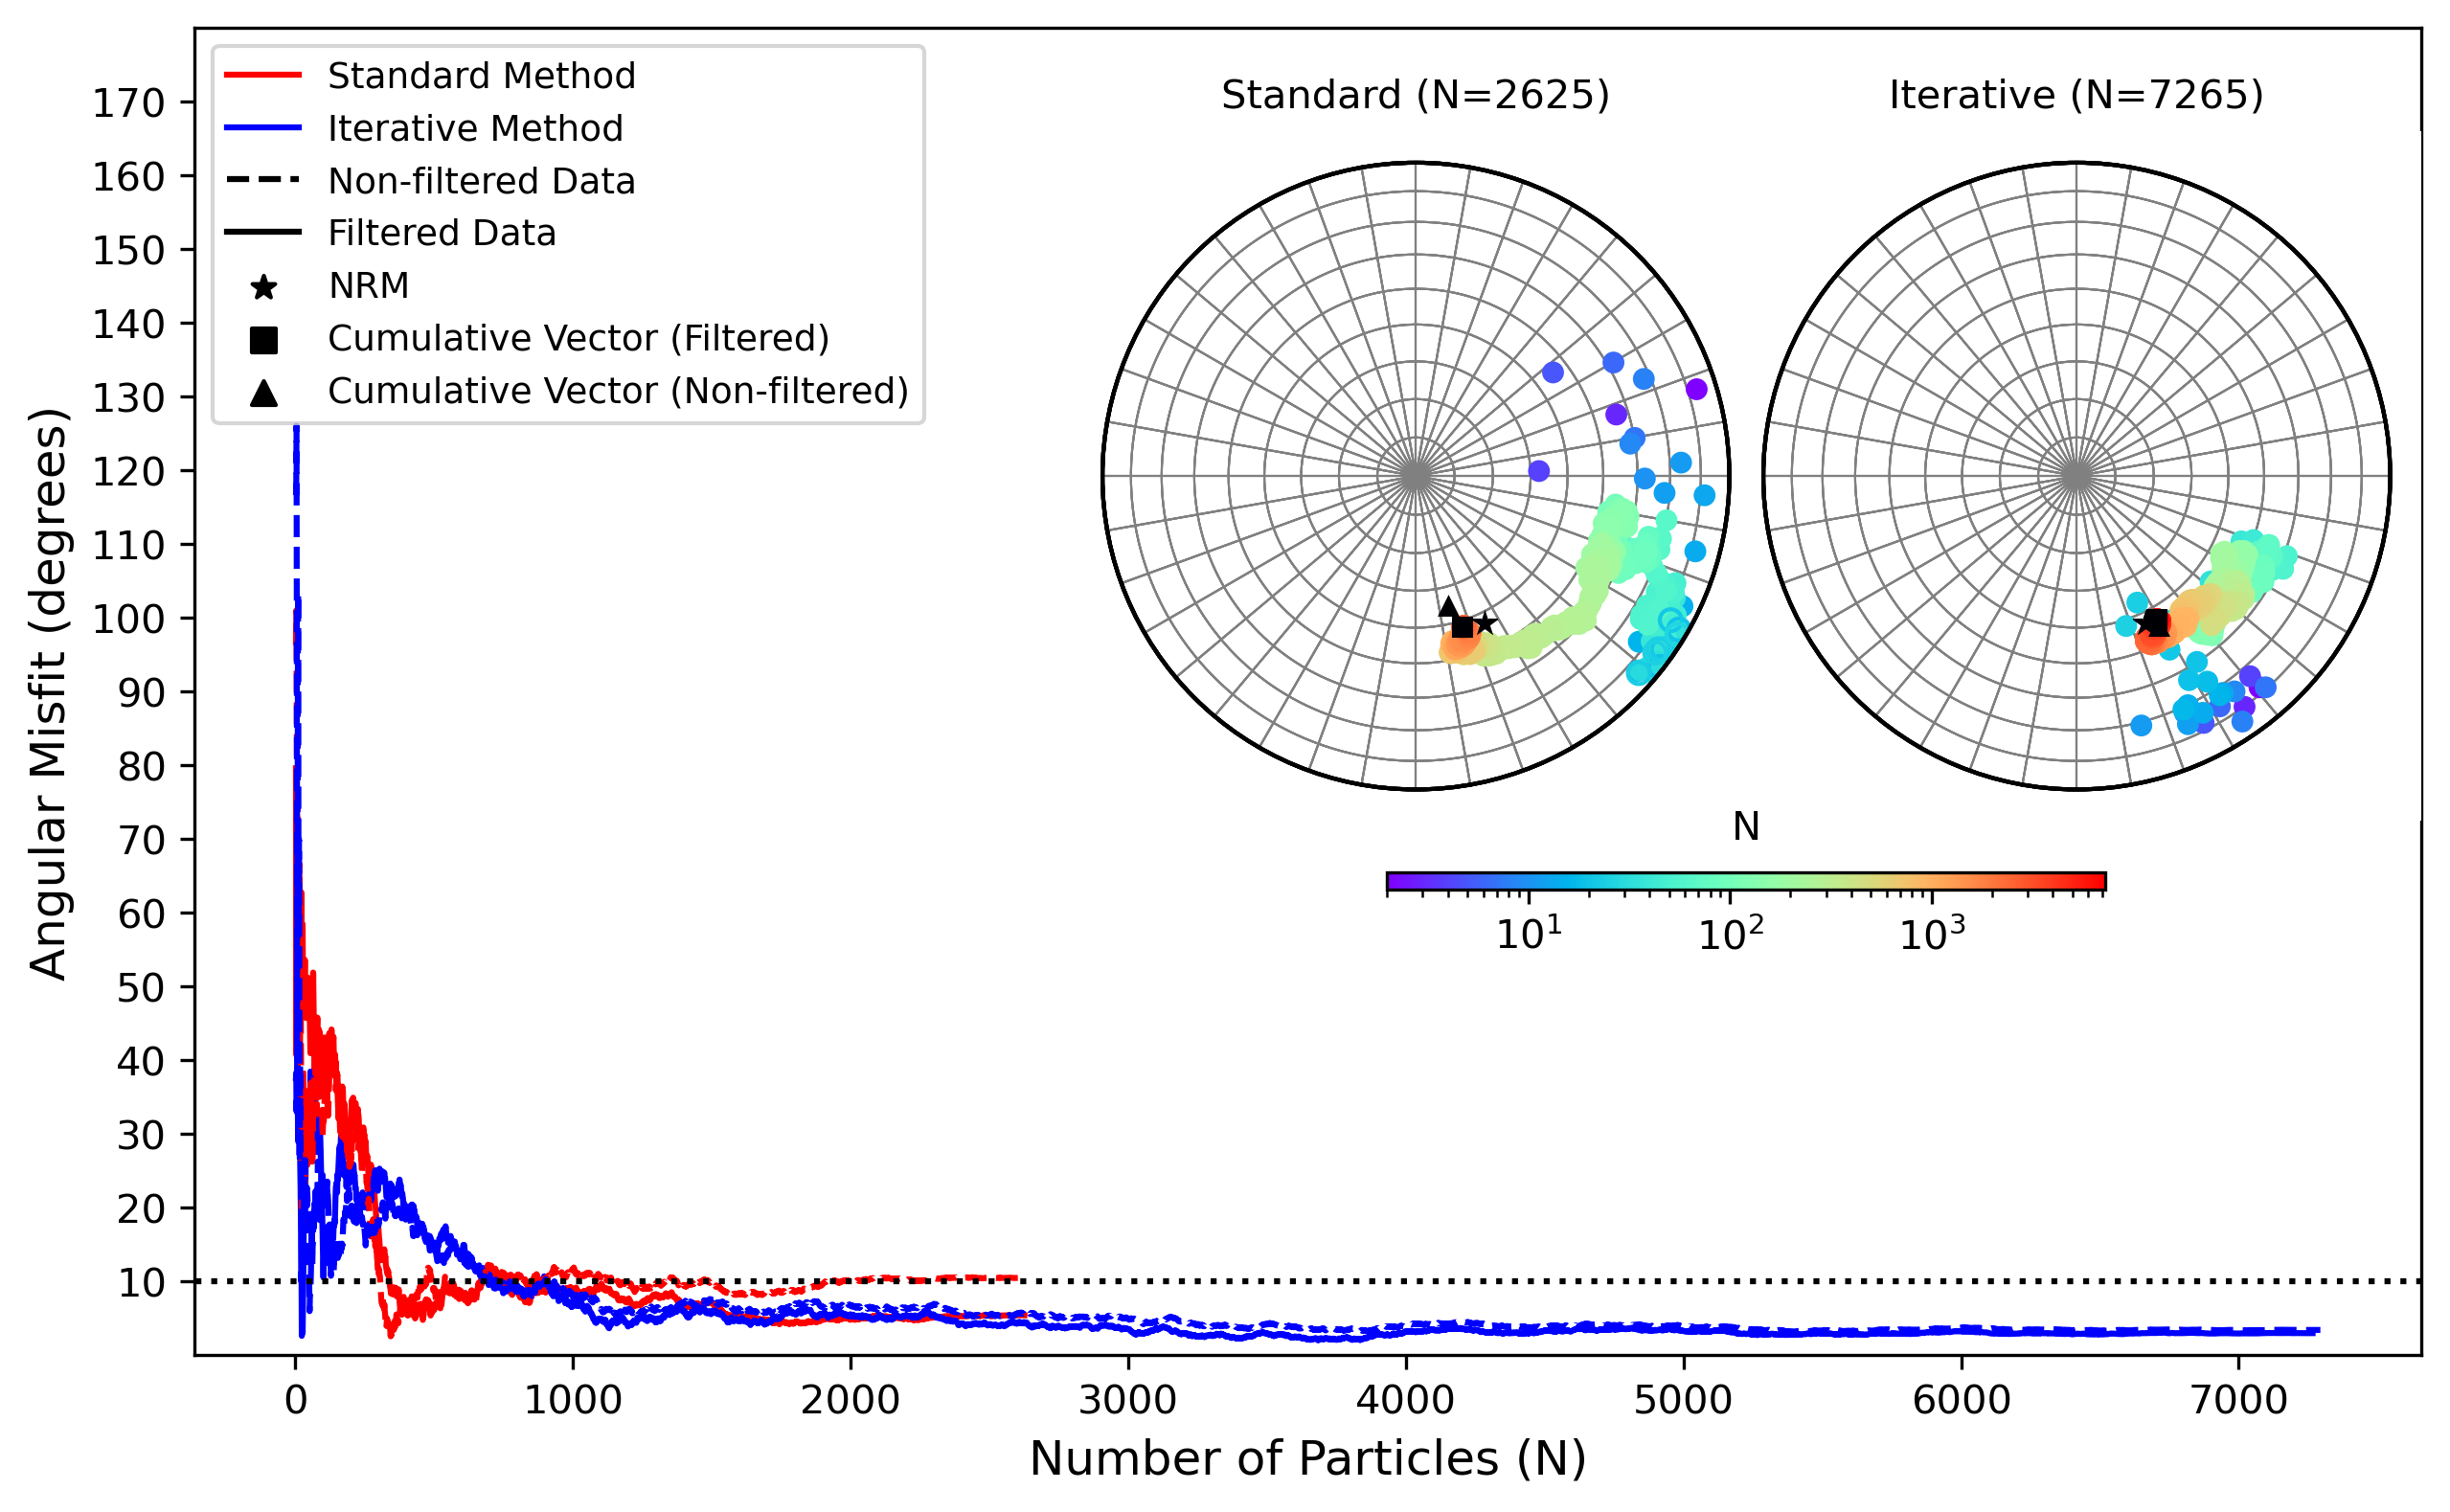
\includegraphics[width=1\linewidth]{micromag-interfering-sources/figures/basalt-data-stereoplot.png}
  \caption{
  Comparison of the standard (red) and iterative (blue) algorithms in reconstructing the NRM direction from the basalt sample. (Left) Angular misfit between the cumulative vector and the measured NRM as a function of the number of particles ($N$). (Right) Stereographic projections of the filtered magnetic vectors ($R^2 \geq 0.9$) for both methods, with the measured NRM (star), non-filtered cumulative direction (triangle), and the filtered cumulative direction (square) indicated. The color gradient denotes the logarithmic scale of particle counts, with warmer colors representing higher concentrations. The solid-lined and dashed-lined curves represent the non-filtered and outliers filtered data, respectively.
  }
  \label{basalt-data-stereograms}
\end{figure}

%%%%%%%%%%%%%%%%%%%%%%%%%%%%%%%%%%%%%%%%%%%%%%%%%%%%%%%%%%%%%%%%%%%%%%%%%%%%%%%
\section{Discussion}

Inverting unique magnetic moment from MM data, regardless of the technique, demands knowing the position of sources. The application of the Euler deconvolution technique emerges to avoid additional measurements, such as nano-tomography, to uncover that information. The isolated windows approach, as justified by \cite{Souza-Junior2024}, enables the separation of the primary signal from the surrounding area using the total gradient anomaly. This method effectively isolates the desired signal while excluding regions outside the window boundaries, which are less sensitive to variations in the magnetic parameters of the specific source. Using this windows approach enables a rapid solution to the inversion problem while keeping it largely overdetermined, since only three parameters are solved per sliced data. However, this thresholding exclusion of the area from the inversion domain violates the basic theory of inversion, which demands that the entire system be considered, ensuring that the interactions between all sources are properly accounted for to obtain a unique and precise solution \citep{Baratchart2013, Lima2013}. Thus, the previous approach of \cite{Souza-Junior2024} will not yield reliable results in all cases. Specifically, in cases influenced by distant sources, even those that are weak, either within the window or close by, which compromises its effectiveness. The latter reflects on a higher amount of results discarded by the filtering criterion.

To tackle these challenges, the iterative method was introduced, providing a more reliable solution for mitigating interference between sources while still preserving the isolated windows approach. Naturally, this comes at the cost of increased inversion time, but the method remains efficient enough to run on a personal computer without demanding massive computational power. Despite the improvements, not all problems have been solved. The new method is more effective at detecting particles and results in more particles passing through the filtering criteria. However, it still faces challenges with inherent limitations of the Euler deconvolution, such as clustered signals. This introduces position estimation errors that are directly influenced by the particle's magnetic signal strength. In particular, errors in vertical position estimation lead to a compensatory trade-off between this positional uncertainty and the recovered dipole intensity. For this reason, our focus here is on the directional aspects of the dataset, while the intensity aspect will require more complex future experiments, along with the implementation of a more refined approach to solving Euler's homogeneity equation, as proposed by \citet{Uieda2025}.

\subsection{Directional recovery assessment}

As noted by \citet{Oliveira2015Estimation}, the least-squares estimator is less sensitive to small errors in particle position and violation of the dipolar assumption when recovering directional information (declination and inclination). This makes the new method particularly effective in refining estimates, increasing the number of results that meet the filtering criteria. As a result, the approach becomes more statistically robust, ultimately improving the overall data quality. The fitting performance was assessed using both synthetic and real datasets, requiring a reliable reference for comparison. In the case of synthetic data, a directional bias (synthetic NRM) was introduced to the dipole magnetic moments based on a spherical distribution. For real samples, the reference direction was obtained from NRM measurements of the whole thin section using the 2G magnetometer.

From the synthetic tests (Figure~\ref{synthetic-data-stereograms}a-c), both the original \citep{Souza-Junior2024} and iterative methods performed well in recovering the directional bias mainly for two reasons. First, dipolar models are generally simpler and tend to produce more results that pass the filtering criteria. Even though the standard method is less efficient in estimating parameters, this deficiency is compensated by the overall behavior of the synthetic sample, and any poor-fitting is treated as random inputs that are effectively removed in the vector sum. The second reason is that, despite a wide distribution of particle moments (from \(10^{-15}\) to \(10^{-11}\)), the stronger particles, which could have further complicated the signal, also followed the bias direction. This contrasts with the overlapping signals synthetic case (Section~\ref{sec:synthetic-overlapping}), where the strong particles were randomly oriented. Nonetheless, it serves as a proxy to isothermal remanent magnetization study cases.

For the real samples, the results in one case deviated from initial expectations. The most dispersed assembly, characterized by a higher proportion of SD/PSD grains and a lower packing density of magnetic particles, exhibited the highest angular misfit, though it remained below 10 degrees (Figure~\ref{ceramic-data-stereograms}). In contrast, the basalt sample produced an angular misfit of less than 5 degrees (Figure~\ref{basalt-data-stereograms}), a result that was not anticipated given the high particle density, particularly the presence of MD grains. This density violates a key assumption of the method, namely that each window should ideally contain a single particle \citep{Souza-Junior2024}. A possible explanation for this positively surprising behavior is provided by recent nanotomography studies of basaltic rocks \citep[\textit{e.g.}][]{Out2024, Out2025}, which have revealed clusters of magnetic particles smaller than \(1~\mu m\). When a window captures such a cluster, the recorded signal represents the sum of the individual contributions. If the cluster exhibits a directional bias, this bias is likely to be reflected in the inversion result. This effect may also account for the improved performance of the standard method in the basaltic sample. While this approach does not effectively resolve interfering sources, it can still capture the overall directional bias of clustered particles, resulting in a lower angular misfit despite the sample’s high particle density.


%%%%%%%%%%%%%%%%%%%%%%%%%%%%%%%%%%%%%%%%%%%%%%%%%%%%%%%%%%%%%%%%%%%%%%%%%%%%%%%
\section{Conclusion}

Our improved algorithm demonstrates substantial advancements over its predecessor, particularly in the context of magnetic microscopy mapping for paleomagnetic studies. By refining the isolation of the primary signal and incorporating an interfering source algorithm, we have enhanced the accuracy of 3D positioning and dipole moment estimations, addressing key limitations of the previous version. These improvements have led to better particle distribution and an increased number of particles meeting the filtering criteria, while also identifying more grains through re-detection. Consequently, the cumulative vector analysis now includes more grains, ensuring statistically reliable direction estimates. This can be achieved with particle counts ranging from several hundred to a few thousand, as demonstrated by both numerical simulations and real data. However, similar conclusions cannot be drawn for intensity studies, as limitations persist in the recovered moment for grains, particularly in clustered particles. Therefore, further research is needed to assess whether this enhanced technique can be applied to paleointensity studies. Despite these challenges, the present work represents a significant advancement in paleomagnetic research at the microscale, owing to the algorithm's ability to recover bulk directional information.

This provides an important step towards paleomagnetism using magnetic microscopy. The possibility of retrieving reliable magnetization directions from thin sections broadens the horizons of previous bulk-derived measurements, such as paleomagnetic tests (e.g., ``conglomerate'' and microscale fold tests). Not only this, we have more capability to spatially correlate the directions estimated (e.g. single crystal inclusion) by obtaining the magnetic information associated with optical images.


\section{Open research}

The Python source code used to produce all results and figures presented here,
as well as supplementary figures and Jupyter notebooks, and the QDM magnetic
microscopy data used in this study are available from \citet{figshare}, which
can also be found on \url{https://github.com/\GitHubRepository} under the MIT
(source code) and CC-BY (data, text, and figures) licenses.

We made use of the following Python software in our research:
scikit-image \citep{VanderWalt2014} for image processing and blob detection;
matplotlib \citep{Hunter2007} for generating figures and stereograms;
Numpy \citep{Harris2020} for basic linear-algebra and array computations;
Scipy \citep{2020SciPy-NMeth} for linear-algebra and non-linear optimization;
Verde \citep{verde2018} for generating data grids;
Harmonica \citep{harmonica2020} for upward continuation and magnetic data processing;
Choclo \citep{choclo2022} for optimized kernel functions used in the
forward and inverse modeling;
Numba \citep{lam2015numba} for just-in-time compilation;
xarray \citep{hoyer2017xarray} for coordinate-aware multidimensional arrays.

%%%%%%%%%%%%%%%%%%%%%%%%%%%%%%%%%%%%%%%%%%%%%%%%%%%%%%%%%%%%%%%%%%%%%%%%%%%%%%%
\section{Acknowledgements}

We gratefully acknowledge the Laboratório de Paleomagnetismo e Magnetismo de Rochas (USPmag, Universidade de São Paulo) for maintaining and providing access to samples, and the Harvard Paleomagnetics Lab (Department of Earth and Planetary Sciences, Harvard University) for providing the facilities and equipment used for the QDM and bulk measurements. We sincerely acknowledge the developers and maintainers of the open-source software, whose contributions were essential to the completion of this work. This research was supported by grants 2021/08379-5 and 2023/13372-5 from the Fundação de Amparo à Pesquisa do Estado de São Paulo (FAPESP), grant IES\textbackslash{}R3\textbackslash{}213141 from the Royal Society, and grant PRPI 22.1.09345.01.2 from Universidade de São Paulo.
The opinions, hypotheses, and conclusions or recommendations expressed in this material are the responsibility of the authors and do not necessarily reflect the views of FAPESP.



\endgroup

%==============================================================================
\chapter{Euler inversion}

\begingroup
% Used to set information about the paper that is used in multiple files
%%%%%%%%%%%%%%%%%%%%%%%%%%%%%%%%%%%%%%%%%%%%%%%%%%%%%%%%%%%%%%%%%%%%%%%%%%%%%%%

% Set variables with the title, authors, etc.
\newcommand{\Title}{Euler inversion: Locating sources of potential-field data through inversion of Euler's homogeneity equation}
\newcommand{\TitleShort}{Euler inversion}

\newcommand{\Year}{2025}
\newcommand{\PreprintOn}{2024/12/19}
\newcommand{\SubmittedOn}{2024/12/20}
\newcommand{\RevisionAOn}{2025/02/28}
\newcommand{\PublishedOn}{2025/03/26}

\newcommand{\Authors}{%
  Leonardo Uieda\textsuperscript{1},
  Gelson Ferreira Souza-Junior\textsuperscript{1},
  India Uppal\textsuperscript{2},
  Vanderlei Coelho Oliveira Jr.\textsuperscript{3}
}
\newcommand{\Affiliations}{%
  \textsuperscript{1} Universidade de São Paulo, Brazil;
  \textsuperscript{2} University of Liverpool, UK;
  \textsuperscript{3} Observatório Nacional, Brazil;
}

\newcommand{\Journal}{Geophysical Journal International}
\newcommand{\JournalDOI}{10.1093/gji/ggaf114}
\newcommand{\PreprintDOI}{10.31223/X5T41M}
\newcommand{\ArchiveDOI}{10.6084/m9.figshare.26384140}
\newcommand{\GitHubRepository}{compgeolab/euler-inversion}
\newcommand{\SWHeritageID}{swh:1:snp:b0d1f8fdbf57f87e0ce56d5dda0f360c4a314d9d}
\newcommand{\SWHeritageURL}{https://archive.softwareheritage.org/\SWHeritageID;origin=https://github.com/\GitHubRepository}

\newcommand{\RioNSources}{\num{300}}
\newcommand{\RioWindowSize}{\qty{12000}{\m}}
\newcommand{\RioWindowStep}{\qty{2400}{\m}}
\newcommand{\RioWeightsF}{\num{1}}
\newcommand{\RioWeightsE}{\num{0.1}}
\newcommand{\RioWeightsN}{\num{0.1}}
\newcommand{\RioWeightsU}{\num{0.05}}
\newcommand{\RioPercentile}{\num{99.5}}
\newcommand{\RioSIMin}{1}
\newcommand{\RioSIMax}{3}\newcommand{\RioNData}{\num{50882}}
\newcommand{\RioDerivSpacing}{\qty{1}{\m}}
\newcommand{\RioEQSDepth}{\qty{1000}{\m}}
\newcommand{\RioEQSDamping}{\num{10}}
\newcommand{\RioEQSBlock}{\qty{100}{\m}}
\newcommand{\RioEQSWindow}{\qty{22313}{\m}}\newcommand{\SynInterfDykesDistMax}{\qty{9000}{\m}}
\newcommand{\SynInterfDykesDistMin}{\qty{1000}{\m}}
\newcommand{\SynInterfDykesTrueEast}{\qty{7000}{\m}}
\newcommand{\SynInterfDykesTrueNorth}{\qty{4500}{\m}}
\newcommand{\SynInterfDykesTrueUp}{\qty{0}{\m}}
\newcommand{\SynInterfDykesTrueBase}{\qty{100}{\nano\tesla}}
\newcommand{\SynInterfDykesInterfEastMax}{\qty{6000}{\m}}
\newcommand{\SynInterfDykesInterfEastMin}{\qty{-2000}{\m}}
\newcommand{\SynInterfDykesInterfNorth}{\qty{4500}{\m}}
\newcommand{\SynInterfDykesInterfUp}{\qty{300}{\m}}
\newcommand{\SynInterfDykesNModels}{33}
\newcommand{\SynInterfDykesInt}{\qty{2e+01}{\ampere\per\meter}}
\newcommand{\SynInterfDykesDec}{\qty{20}{\degree}}
\newcommand{\SynInterfDykesInc}{\qty{-30}{\degree}}
\newcommand{\SynInterfDykesHeight}{\qty{400}{\m}}
\newcommand{\SynInterfDykesSpacing}{\qty{150}{\m}}\newcommand{\SynInterfTrueEast}{\qty{7000}{\m}}
\newcommand{\SynInterfTrueNorth}{\qty{4000}{\m}}
\newcommand{\SynInterfTrueUp}{\qty{-3000}{\m}}
\newcommand{\SynInterfTrueBase}{\qty{100}{\nano\tesla}}
\newcommand{\SynInterfInterfEastMax}{\qty{5000}{\m}}
\newcommand{\SynInterfInterfEastMin}{\qty{-1000}{\m}}
\newcommand{\SynInterfInterfNorth}{\qty{5000}{\m}}
\newcommand{\SynInterfInterfUp}{\qty{-1500}{\m}}
\newcommand{\SynInterfNModels}{31}
\newcommand{\SynInterfInt}{\qty{5e+11}{\ampere\per\meter}}
\newcommand{\SynInterfDec}{\qty{-10}{\degree}}
\newcommand{\SynInterfInc}{\qty{-30}{\degree}}
\newcommand{\SynInterfHeight}{\qty{400}{\m}}
\newcommand{\SynInterfSpacing}{\qty{200}{\m}}\newcommand{\SynNoiseWeightsF}{1}
\newcommand{\SynNoiseWeightsE}{0.1}
\newcommand{\SynNoiseWeightsN}{0.1}
\newcommand{\SynNoiseWeightsU}{0.025}
\newcommand{\SynNoiseTrueEast}{\qty{15000}{\m}}
\newcommand{\SynNoiseTrueNorth}{\qty{11000}{\m}}
\newcommand{\SynNoiseTrueUp}{\qty{-5000}{\m}}
\newcommand{\SynNoiseTrueBase}{\qty{100}{\nano\tesla}}
\newcommand{\SynNoiseInt}{\qty{2e+12}{\ampere\per\meter}}
\newcommand{\SynNoiseDec}{\qty{15}{\degree}}
\newcommand{\SynNoiseInc}{\qty{-30}{\degree}}
\newcommand{\SynNoiseMin}{\qty{0}{\nano\tesla}}
\newcommand{\SynNoiseMax}{\qty{40}{\nano\tesla}}
\newcommand{\SynNoiseStep}{\qty{0.2}{\nano\tesla}}
\newcommand{\SynNoisePlotted}{0, 10, 25, and \qty{40}{\nano\tesla}}
\newcommand{\SynNoiseHeight}{\qty{800}{\m}}
\newcommand{\SynNoiseSpacing}{\qty{500}{\m}}
\newcommand{\SynNoiseErrUEI}{\qty{4628}{\m}}
\newcommand{\SynNoiseErrUED}{\qty{4252}{\m}}
\newcommand{\SynNoiseErrUEIW}{\qty{2128}{\m}}
\newcommand{\SynNoiseErrNEI}{\qty{81}{\m}}
\newcommand{\SynNoiseErrNED}{\qty{449}{\m}}
\newcommand{\SynNoiseErrNEIW}{\qty{125}{\m}}
\newcommand{\SynNoiseErrEEI}{\qty{947}{\m}}
\newcommand{\SynNoiseErrEED}{\qty{1275}{\m}}
\newcommand{\SynNoiseErrEEIW}{\qty{482}{\m}}
\newcommand{\SynNoiseErrBEI}{\qty{10}{\nano\tesla}}
\newcommand{\SynNoiseErrBED}{\qty{4}{\nano\tesla}}
\newcommand{\SynNoiseErrBEIW}{\qty{9}{\nano\tesla}}\newcommand{\DefaultWeightsF}{1}
\newcommand{\DefaultWeightsE}{0.1}
\newcommand{\DefaultWeightsN}{0.1}
\newcommand{\DefaultWeightsU}{0.025}
\newcommand{\SynProofTrueEast}{\qty{15000}{\m}}
\newcommand{\SynProofTrueNorth}{\qty{12000}{\m}}
\newcommand{\SynProofTrueUp}{\qty{-3000}{\m}}
\newcommand{\SynProofTrueBase}{\qty{100}{\nano\tesla}}
\newcommand{\SynProofInt}{\qty{5e+11}{\ampere\per\meter}}
\newcommand{\SynProofDec}{\qty{15}{\degree}}
\newcommand{\SynProofInc}{\qty{-30}{\degree}}
\newcommand{\SynProofNoise}{\qty{10}{\nano\tesla}}
\newcommand{\SynProofHeight}{\qty{800}{\m}}
\newcommand{\SynProofSpacing}{\qty{300}{\m}}
\newcommand{\SynProofEstEast}{\qty{15045}{\m}}
\newcommand{\SynProofEstNorth}{\qty{12028}{\m}}
\newcommand{\SynProofEstUp}{\qty{-2663}{\m}}
\newcommand{\SynProofEstBase}{\qty{93}{\nano\tesla}}
\newcommand{\SynProofEDEast}{\qty{14626}{\m}}
\newcommand{\SynProofEDNorth}{\qty{11865}{\m}}
\newcommand{\SynProofEDUp}{\qty{-1553}{\m}}
\newcommand{\SynProofEDBase}{\qty{94}{\nano\tesla}}
\newcommand{\SynProofNIter}{6}\newcommand{\DefaultSIMin}{0}
\newcommand{\DefaultSIMax}{3}
\newcommand{\SynSITrueEast}{\qty{15000}{\m}}
\newcommand{\SynSITrueNorth}{\qty{10000}{\m}}
\newcommand{\SynSITrueUp}{\qty{0}{\m}}
\newcommand{\SynSITrueBase}{\qty{300}{\nano\tesla}}
\newcommand{\SynSIDec}{\qty{-20}{\degree}}
\newcommand{\SynSIInc}{\qty{35}{\degree}}
\newcommand{\SynSINoise}{\qty{15}{\nano\tesla}}
\newcommand{\SynSIHeight}{\qty{1000}{\m}}
\newcommand{\SynSISpacing}{\qty{300}{\m}}\newcommand{\SynWinDec}{\qty{-20}{\degree}}
\newcommand{\SynWinInc}{\qty{-30}{\degree}}
\newcommand{\SynWinNoise}{\qty{50}{\nano\tesla}}
\newcommand{\SynWinBase}{\qty{1000}{\nano\tesla}}
\newcommand{\SynWinHeight}{\qty{1000}{\m}}
\newcommand{\SynWinSpacing}{\qty{500}{\m}}
\newcommand{\SynWinWindowSize}{\qty{10000}{\m}}
\newcommand{\SynWinWindowStep}{\qty{5000}{\m}}
\newcommand{\SynWinNSources}{10}
\newcommand{\SynWinKeepED}{0.3}
\newcommand{\SynWinKeepFD}{0.35}
\newcommand{\SynWinKeepEI}{0.25}
\newcommand{\SynWinRegionalE}{\qty{0.02}{\nano\tesla\per\meter}}
\newcommand{\SynWinRegionalN}{\qty{-0.03}{\nano\tesla\per\meter}}

\begin{summarybox}
    \noindent
    This chapter was originally published as
    \textbf{``Uieda, L., Souza-Junior, G. F., Uppal, I. and Oliveira Jr., V. C.
    (\Year). \Title{}. \textit{\Journal{}}.
    doi:\href{https://doi.org/\JournalDOI}{\JournalDOI}.''} under the
    terms of the CC-BY license. It is reproduced here under these terms.
\end{summarybox}

\section*{Abstract}
Locating the sources of observed disturbances in potential-field data is a challenging problem due to the non-unique nature of the inverse problem.
The Euler deconvolution method was created to solve this issue, particularly for idealized sources (such as spheres and planar vertical dykes).
Euler deconvolution has become widely used in potential-field methods due, in large part, to its low computational cost and ease of implementation into software.
However, it is widely known that Euler deconvolution suffers from some shortcomings: 1) non-uniqueness of the solution with respect to the depth of the source and the structural index (a parameter that represents the idealised shape of the source); 2) sensitivity to short-wavelength noise in the data derivatives which are used as inputs for the method.
Here, we present a new method called \textit{Euler inversion} which is a reformulation of the inverse problem of Euler's homogeneity equation as an implicit mathematical model rather than a parametric one.
Euler inversion is a constrained, non-linear inverse problem capable of estimating both the model parameters (location of the source and constant base level) and the predicted data (potential field and its derivatives).
We show that Euler inversion is less sensitive than Euler deconvolution to short-wavelength noise and to the presence of interfering sources in the data window.
By also estimating the predicted data, Euler inversion is also able to estimate the best integer structural index
to be used for inversion.
Our results show that the estimated structural index minimizes the data misfit and coincides with those of the simulated sources.
Furthermore, most matrices involved in the method are either sparse or diagonal, making Euler inversion computationally efficient.
Tests on synthetic data and a real aeromagnetic dataset from Rio de Janeiro, Brazil, demonstrate the effectiveness of Euler inversion to delineate sources with variable geometries and correctly estimate their depths.


% \section{Introduction}

Estimating the depths of the sources of measured anomalies is a common
challenge in potential-field geophysics.
One of the most widely used techniques for providing depth estimates is Euler
deconvolution \citep{Thompson1982,Reid1990}.
Its widespread adoption is due, in large part, to its low algorithmic
complexity and fast computation times, both of which are orders of magnitude
smaller than solutions from 3D inverse problems.
As a result, Euler deconvolution is widely available in both commercial and
open-source software \citep{Uieda2013,Uieda2014}.
Unfortunately, this popularity has also led to abuses of the method, as
reported in \citet{Reid2014} and \citet{Reid2014b}.

Euler deconvolution is a method that assumes potential-field data are generated
by idealized sources, such as dikes, dipoles, or pipes.
The geometry of these sources is characterized by the structural index,
a parameter that must be an integer to retain physical significance
\citep{Stavrev2007,Reid2014}.
The technique involves performing a least-squares inversion of Euler's
homogeneity equation multiple times, in a moving window scheme.
Each inversion estimates the base level, a constant shift in the data, and also
the coordinates of a single idealized source potentially present within the
study area.

It is well known that Euler deconvolution suffers from some limitations, of
which we highlight:

\begin{enumerate}

\item \textbf{Separation of reliable and spurious solutions:} The moving window
    scheme adopted in Euler deconvolution generates many estimated positions
    which are considered spurious and must be removed. Most of the spurious
    solutions happen when the moving window either lacks significant
    potential-field anomalies or only contains a truncated anomaly.
    \citet{FitzGerald2004} and \citet{Melo2020} provide overviews of the many
    existing methods that have been developed to remove spurious solutions.

\item \textbf{Sensitivity to high-frequency noise:}
    Random noise in the data is
    usually of high-frequency, which gets amplified in the derivative
    calculations. Since the field derivatives are used in the Jacobian matrix
    of the least-squares inversions, errors in the derivatives will have
    a large impact on the solution. \citet{Pasteka2009}, \citet{Saleh2012}, and
    \citet{Florio2014} recommend using regularised derivatives or other
    smoothing techniques to reduce the noise amplification and obtain more
    reliable solutions. This is also why Euler deconvolution variants that rely
    on higher-order derivatives, like tilt-Euler deconvolution
    \citep{Salem2007,Huang2019} and AN-EUL \citep{Salem2003}, present a larger
    dispersion of estimated positions and are more sensitive to noise in
    general. Methods like finite-difference Euler deconvolution
    \citep{Gerovska2005} and ratio-Euler deconvolution \citep{Huang2022} were
    specifically developed to avoid the use of higher-order derivatives because
    of this noise-sensitivity issue.

\item \textbf{Correlation of the estimated depth and the structural index:}
    \citet{Silva2001} demonstrated that the estimated depth from Euler
    deconvolution is directly correlated with the structural index used. The
    higher the structural index, the larger the estimated depth. This makes it
    very important to know the best integer structural index for the type of
    source being interpreted. Some Euler deconvolution variants have been
    developed that are able to estimate the structural index
    \citep[e.g.,][]{Melo2013,Melo2018,Salem2003,Salem2007,Gerovska2005,Silva2003,Florio2013,Florio2014}.
    However, most of them estimate real-valued structural indices instead of
    integers, are sensitive to noise, and tend to underestimate the structural
    index under realistic noise and signal overlap scenarios.
    Another approach is that of \citet{Mushayandebvu2004}, who exploit the
    ill-conditioning of the Jacobian matrix of Euler deconvolution to detect
    the presence of 2D sources (structural index of one for magnetic data and
    0 for gravity data) in a data window and correctly estimate their
    position and strike.

\end{enumerate}

Euler deconvolution and its variants are also know to struggle with models that
have two or more contact points, like steps which have a top and a bottom.
To solve this problem, methods like MaGSoundFDST method of
\citet{Gerovska2010} were developed based on the similarity transform.
MaGSoundFDST, in particular, is able to estimate structural index, source
locations, and the number of sources, hence side-stepping the problem of
spurious solutions altogether.


We aim to tackle some of these issues by reformulating the inverse problem of
solving Euler's homogeneity equation.
The issue of noise sensitivity can be traced back to the presence of data
derivatives in the Jacobian matrix, which generally contain larger amounts of
noise than the original potential field.
We propose formulating the inverse problem as a non-linear optimisation with
Euler's equation as a constraint.
This is similar to ``total least-squares'' in statistics \citep{VanHuffel1991}
and ``combined adjustment'' in geodesy \citep{Vanicek1986}.
Another advantage of this new formulation is the ability to calculate predicted
data for the potential-field and its three derivatives, which is impossible in
Euler deconvolution and all of its variants.
We call our new method ``Euler inversion''.

%%%%%%%%%%%%%%%%%%%%%%%%%%%%%%%%%%%%%%%%%%%%%%%%%%%%%%%%%%%%%%%%%%%%%%%%%%%%%%%
\section{Methodology}

Starting with \citet{Thompson1982} and \citet{Reid1990}, Euler's equation has
been used to estimate the source positions of gravity and magnetic data.
In this section, we will review the solution of Euler's equation for the source
location $(x_o, y_o, z_o)$ by Euler deconvolution \citep{Reid1990} and then
present a new method, called \textit{Euler inversion}, for solving Euler's
equation using total least-squares.

We start with Euler's homogeneity equation

\begin{equation}
  (x - x_o)\partial_x f + (y - y_o)\partial_y f + (z - z_o)\partial_z f
  + \eta(f - b) = 0
  \ ,
  \label{eq:euler}
\end{equation}

\noindent
in which $f$ is a homogeneous function (in this case, a potential-field),
$\partial_\alpha$ is the derivative operator in the $\alpha$ direction,
$(x, y, z)$ are the coordinates of the observation point,
$(x_o, y_o, z_o)$ are the coordinates of the field source,
$b$ is the base level representing a constant shift in the field,
and $\eta$ is the structural index, which is related to the nature of the
source and how its potential-field values decay with distance
\citep{Ruddock1966,Reid2014}.
The coordinate system is defined with $x$ pointing eastward, $y$ pointing northward, and $z$ pointing upward.
Equation~\ref{eq:euler} relates the coordinates of the source with the
potential field and its gradient observed at the point $(x, y, z)$.

Given $N$ observations points in which we have measured $f$ and its gradient
(for a total $4N$ data), we can define the system of $N$ equations and $4$
unknowns

\begin{equation}
  \begin{aligned}
    (x_1-x_o)\partial_x f_1 + (y_1-y_o)\partial_y f_1 + (z_1-z_o)\partial_z f_1 + \eta(f_1-b) &= 0
    \\
    (x_2-x_o)\partial_x f_2 + (y_2-y_o)\partial_y f_2 + (z_2-z_o)\partial_z f_2 + \eta(f_2-b) &= 0
    \\
    \vdots
    \\
    (x_N-x_o)\partial_x f_N + (y_N-y_o)\partial_y f_N + (z_N-z_o)\partial_z f_N + \eta(f_N-b) &= 0
  \end{aligned}
  \ .
  \label{eq:euler-system}
\end{equation}

\noindent
Both Euler deconvolution and Euler inversion aim to solve the equation system
above to estimate the parameter vector

\begin{equation}
  \mathbf{p} = \begin{bmatrix}x_o & y_o & z_o & b \end{bmatrix}^T.
  \label{eq:p}
\end{equation}


\subsection{Euler deconvolution}

Euler deconvolution starts by rearranging Equation~\ref{eq:euler-system} to
place the parameters on the left-hand side and all other terms on the
right-hand side. This is an attempt to form a \textit{parametric model} which
results in the equation system

\begin{equation}
  \begin{aligned}
  -x_o\partial_x f_1 - y_o\partial_y f_1 - z_o\partial_z f_1 - \eta b &= -x_1\partial_x f_1 - y_1\partial_y f_1 - z_1\partial_z f_1 - \eta f_1
  \\
  -x_o\partial_x f_2 - y_o\partial_y f_2 - z_o\partial_z f_2 - \eta b &= -x_2\partial_x f_2 - y_2\partial_y f_2 - z_2\partial_z f_2 - \eta f_2
  \\
  \vdots
  \\
  -x_o\partial_x f_N - y_o\partial_y f_N - z_o\partial_z f_N - \eta b &= -x_N\partial_x f_N - y_N\partial_y f_N - z_N\partial_z f_N - \eta f_N
  \end{aligned}
  \ ,
\end{equation}

\noindent
which can be written in matrix form as

\begin{equation}
  \underbrace{
    \begin{bmatrix}
      -\partial_x f_1 & -\partial_y f_1 & -\partial_z f_1 & -\eta \\
      -\partial_x f_2 & -\partial_y f_2 & -\partial_z f_2 & -\eta \\
      \vdots & \vdots & \vdots & \vdots \\
      -\partial_x f_N & -\partial_y f_N & -\partial_z f_N & -\eta
    \end{bmatrix}
  }_{\mathbf{A}}
  \underbrace{
    \begin{bmatrix}
      x_o \\ y_o \\ z_o \\ b
    \end{bmatrix}
  }_{\mathbf{p}}
  =
  \underbrace{
    \begin{bmatrix}
      -x_1\partial_x f_1 - y_1\partial_y f_1 - z_1\partial_z f_1 - \eta f_1 \\
      -x_2\partial_x f_2 - y_2\partial_y f_2 - z_2\partial_z f_2 - \eta f_2 \\
      \vdots \\
      -x_N\partial_x f_N - y_N\partial_y f_N - z_N\partial_z f_N - \eta f_N \\
    \end{bmatrix}
  }_{\mathbf{c}}
  \ ,
  \label{eq:deconv-system}
\end{equation}

\noindent
in which $\mathbf{A}$ is the Jacobian matrix of Euler's equation
(Equation~\ref{eq:euler}) concerning the parameters
(Equations~\ref{eq:p})
and $\mathbf{c}$ is a \textit{pseudo-data vector}.

The solution proposed by \citet{Thompson1982} and \citet{Reid1990} is a
least-squares estimate of $\mathbf{p}$

\begin{equation}
  \mathbf{p} = \left(\mathbf{A}^T\mathbf{A}\right)^{-1}
  \mathbf{A}^T\mathbf{c}
  \ .
  \label{eq:deconv-p}
\end{equation}

\noindent
The covariance matrix of the parameters $\mathbf{C}_p$ is obtained through
standard error propagation assuming that the only variable with uncertainty
is the pseudo-data vector $\mathbf{c}$

\begin{equation}
  \mathbf{C}_p = \hat{\sigma}_0^2 \left(\mathbf{A}^T\mathbf{A}\right)^{-1}
  \ ,
  \label{eq:deconv-cov}
\end{equation}

\noindent
in which
${\hat{\sigma}_0^2} = \|\mathbf{c} - \mathbf{A}\mathbf{p}\|^2 / (N - 4)$
is the reduced chi-squared statistic and an estimate of the variance factor of
$\mathbf{c}$.

The solution in Equation~\ref{eq:deconv-p} above is valid only if the
contents of the Jacobian matrix $\mathbf{A}$ are assumed to be error-free.
As can be seen from Equation~\ref{eq:deconv-system}, the Jacobian contains the
derivatives of $f$, which are often computed numerically by finite-differences
or Fourier transforms and are known to amplify the high-frequency random noise
in the data.
This presents a problem, particularly for the estimation of $z_o$, which has
been widely explored in the literature
\citep{Silva2001,Melo2020,Pasteka2009,Florio2014}.


\subsection{Euler inversion: Formulation}

Euler inversion starts by assigning the potential-field $f$ to a $N \times 1$
vector

\begin{equation}
  \mathbf{f} =
  \begin{bmatrix}
    f_1 & f_2 & \cdots & f_N
  \end{bmatrix}^T.
\end{equation}

\noindent
We can then define a $4N \times 1$ \textit{data vector} which contains all of
the values of $f$ and its gradient

\begin{equation}
  \mathbf{d} =
  \begin{bmatrix}
    \mathbf{f}^T
    & \mathbf{\nabla}_x\mathbf{f}^T
    & \mathbf{\nabla}_y\mathbf{f}^T
    & \mathbf{\nabla}_z\mathbf{f}^T
  \end{bmatrix}^T.
  \label{eq:d}
\end{equation}

\noindent
in which $\mathbf{\nabla}_\alpha$ is the gradient operator in the $\alpha$
dimension.

Next, we formulate the $N \times 4$ equation system
from Euler's equation
(Equation~\ref{eq:euler-system})
as a non-linear function of both parameters and data

\begin{equation}
  \mathbf{e}(\mathbf{p}, \mathbf{d}) = \mathbf{0}
  \ ,
  \label{eq:e}
\end{equation}

\noindent
which is known in geodesy as an \textit{implicit mathematical model}
\citep{Vanicek1986}.

We then wish to solve the following constrained optimisation problem with
non-linear equality constraints to estimate both the parameters and the
predicted data simultaneously

\begin{equation}
  \begin{aligned}
    \min_{\mathbf{p}, \mathbf{d}} \quad &
      \phi(\mathbf{d}) =
      \left[\mathbf{d}^o - \mathbf{d}\right]^T \mathbf{W}
      \left[\mathbf{d}^o - \mathbf{d}\right]
    \\
    \textrm{subject to} \quad &
      \mathbf{e}(\mathbf{p}, \mathbf{d}) = \mathbf{0}
    \ ,
  \end{aligned}
  \label{eq:constrained}
\end{equation}

\noindent
in which $\mathbf{d}^o$ is the \textit{observed data vector} which contains all
of the $4N$ observations of $f$ and its gradient,
$\mathbf{d}$ is the \textit{predicted data vector} from Equation~\ref{eq:d},
and $\mathbf{W}$ is a $4N \times 4N$ diagonal weight matrix.
The first $N$ terms of the diagonal of $\mathbf{W}$ are the weights for the
potential field observations and the following $3N$ terms are the weights of
x-, y-, and z-derivatives of the potential field, in order.
In practice, the weight matrix is usually diagonal because covariances of
observations are seldom available.
The weights can be used to reduce the importance of each datum in the
fitting process, allowing for mitigation of outliers or data components that
have higher levels of noise.

The constrained problem in Equation~\ref{eq:constrained} can be transformed
into an unconstrained problem by using the Lagrangian

\begin{equation}
  \Lagr(\mathbf{p}, \mathbf{d}, \boldsymbol{\lambda}) =
    \left[\mathbf{d}^o - \mathbf{d}\right]^T \mathbf{W}
    \left[\mathbf{d}^o - \mathbf{d}\right]
    +
    2 \boldsymbol{\lambda}^T \mathbf{e}
  \ ,
  \label{eq:lagrangian}
\end{equation}

\noindent
in which $\boldsymbol{\lambda}$ is an $N \times 1$ vector of Lagrange
multipliers.
The non-linear Lagrangian is minimised through Newton's method
\citep{Aster2019}.
We start with initial estimates $\mathbf{p}_0$ and $\mathbf{d}_0$ and then
iteratively apply corrections $\mathbf{\Delta p}_k$ and $\mathbf{\Delta d}_k$
until convergence is achieved.
To calculate the corrections, we introduce a new variable $\mathbf{u} =
[\mathbf{d}^T\  \boldsymbol{\lambda}^T \ \mathbf{p}^T]^T$, expand the
Lagrangian $\Lagr(\mathbf{u})$ (Equation~\ref{eq:lagrangian}) in a Taylor
series around point $\mathbf{u}_k$, and disregard terms of order higher than
two

\begin{equation}
  \Lagr(\mathbf{u}) \approx
  \Gamma(\mathbf{u}) =
  \Lagr(\mathbf{u}_k)
    + \mathbf{\Delta u}_k^T \mathbf{\nabla}\Lagr(\mathbf{u}_k)
    + \dfrac{1}{2}\mathbf{\Delta u}_k^T\mathbf{H}_k\mathbf{\Delta u}_k
  \ ,
  \label{eq:taylor}
\end{equation}

\noindent
in which $\mathbf{\nabla}$ is the gradient operator and $\mathbf{H}_k$ is the
Hessian matrix of $\Lagr$ evaluated at $\mathbf{u}_k$.
Equation~\ref{eq:taylor} is a quadratic function of $\mathbf{\Delta u}_k$ and
we can obtain its minimum by taking its gradient and equating it to the null
vector

\begin{equation}
  \begin{gathered}
    \mathbf{\nabla}\Gamma(\mathbf{\Delta u}_k) =
      \mathbf{\nabla}\Lagr(\mathbf{u_k})
      + \mathbf{H}_k\mathbf{\Delta u}_k
      = \mathbf{0}
    \ ,
    \\
    \mathbf{H}_k\mathbf{\Delta u}_k = -\mathbf{\nabla}\Lagr(\mathbf{u_k})
    \ .
  \end{gathered}
\end{equation}

\noindent
The equation above is the \textit{system of normal equations}, which can also
be written in terms of $\mathbf{p}$, $\boldsymbol{\lambda}$, and $\mathbf{d}$

\begin{equation}
  \underbrace{
    \begin{bmatrix}
      \mathbf{H}^{dd}_k & \mathbf{H}^{d\lambda}_k & \mathbf{H}^{dp}_k \\
      \mathbf{H}^{\lambda d}_k & \mathbf{H}^{\lambda\lambda}_k & \mathbf{H}^{\lambda p}_k \\
      \mathbf{H}^{pd}_k & \mathbf{H}^{p\lambda}_k & \mathbf{H}^{pp}_k
    \end{bmatrix}
  }_{\text{Hessian of }\Lagr}
  \underbrace{
    \begin{bmatrix}
      \mathbf{\Delta d}_k \\
      \boldsymbol{\Delta\lambda}_k \\
      \mathbf{\Delta p}_k
    \end{bmatrix}
  }_{\mathbf{\Delta u}_k}
  = -
  \underbrace{
    \begin{bmatrix}
      \mathbf{\nabla}_d\Lagr(\mathbf{p}_k,\mathbf{d}_k,\boldsymbol{\lambda}_k) \\
      \mathbf{\nabla}_\lambda\Lagr(\mathbf{p}_k,\mathbf{d}_k,\boldsymbol{\lambda}_k) \\
      \mathbf{\nabla}_p\Lagr(\mathbf{p}_k,\mathbf{d}_k,\boldsymbol{\lambda}_k)
    \end{bmatrix}
  }_{\text{gradient of }\Lagr}
  \ ,
\end{equation}

\noindent
in which $\mathbf{\nabla}_\alpha$ is the gradient operator with respect to
variable $\alpha$ and
$\mathbf{H}_k^{\alpha\beta}$ is the Hessian matrix of $\Lagr$ with respect to
variables $\alpha$ and $\beta$, evaluated at $\mathbf{u}_k$.
Since the order of derivation can be swapped in the Hessian matrices and the
Hessian of $\Lagr$ is symmetric, the above equation can be simplified to

\begin{equation}
    \begin{bmatrix}
      \mathbf{H}^{dd}_k & \mathbf{H}^{d\lambda}_k & \mathbf{H}^{dp}_k \\
      {\mathbf{H}^{d\lambda}_k}^T & \mathbf{H}^{\lambda\lambda}_k & \mathbf{H}^{\lambda p}_k \\
      {\mathbf{H}^{dp}_k}^T & {\mathbf{H}^{\lambda p}_k}^T & \mathbf{H}^{pp}_k
    \end{bmatrix}
  \begin{bmatrix}
    \mathbf{\Delta d}_k \\
    \boldsymbol{\Delta\lambda}_k \\
    \mathbf{\Delta p}_k
  \end{bmatrix}
  = -
    \begin{bmatrix}
      \mathbf{\nabla}_d\Lagr(\mathbf{p}_k,\mathbf{d}_k,\boldsymbol{\lambda}_k) \\
      \mathbf{\nabla}_\lambda\Lagr(\mathbf{p}_k,\mathbf{d}_k,\boldsymbol{\lambda}_k) \\
      \mathbf{\nabla}_p\Lagr(\mathbf{p}_k,\mathbf{d}_k,\boldsymbol{\lambda}_k)
    \end{bmatrix}
  \ .
  \label{eq:newton}
\end{equation}

Now, we must derive the three gradient vectors and six Hessian matrices in
Equation~\ref{eq:newton}.
We will start with the gradient vectors.

\begin{equation}
  \begin{aligned}
    \mathbf{\nabla}_d\Lagr(\mathbf{p}_k,\mathbf{d}_k,\boldsymbol{\lambda}_k) &=
      2\left(-\mathbf{W}\left[\mathbf{d}^o - \mathbf{d}_k\right]
      + \mathbf{B}_k^T\boldsymbol{\lambda}_k\right)
    \ ,
    \\
    \mathbf{\nabla}_\lambda\Lagr(\mathbf{p}_k,\mathbf{d}_k,\boldsymbol{\lambda}_k) &=
      2\mathbf{e}_k
    \ ,
    \\
    \mathbf{\nabla}_p\Lagr(\mathbf{p}_k,\mathbf{d}_k,\boldsymbol{\lambda}_k) &=
      2\mathbf{A}_k^T\boldsymbol{\lambda}_k
    \ ,
  \end{aligned}
  \label{eq:grad}
\end{equation}

\noindent
in which $\mathbf{e}_k = \mathbf{e}(\mathbf{p}_k,\mathbf{d}_k)$
(Equation~\ref{eq:e}), $\mathbf{A}_k$ is the $N \times 4$ \textit{parameter
Jacobian} matrix of Euler's equation (Equation~\ref{eq:deconv-system})
evaluated on $(\mathbf{p}_k,\mathbf{d}_k)$, and $\mathbf{B}_k$ is the $N \times
4N$ \textit{data Jacobian} of Euler's equation, also evaluated on
$(\mathbf{p}_k,\mathbf{d}_k)$.
The data Jacobian $\mathbf{B}_k$ contains the first derivatives of Euler's
equation (Equation~\ref{eq:euler})
with respect to the data vector $\mathbf{d}$ (Equation~\ref{eq:d}).
It is composed of four diagonal matrices

\begin{equation}
  \mathbf{B}_k =
  \begin{bmatrix}
    \mathbf{B}^f_k &
    \mathbf{B}^x_k &
    \mathbf{B}^y_k &
    \mathbf{B}^z_k
  \end{bmatrix}
  \ .
  \label{eq:B}
\end{equation}

\noindent
The diagonal elements of each of the four matrices are

\begin{equation}
  \begin{aligned}
    {B^f_k}_{ii} &= \eta \ , &
    {B^x_k}_{ii} &= x_i - {x_o}_k \ , &
    {B^y_k}_{ii} &= y_i - {y_o}_k \ , &
    {B^z_k}_{ii} &= z_i - {z_o}_k \ .
  \end{aligned}
\end{equation}

The Hessian matrices are calculated using a Gauss-Newton approximation
disregarding second-order derivatives. The six independent Hessians are given
by

\begin{equation}
  \begin{aligned}
    \mathbf{H}^{dd}_k &\approx 2\mathbf{W} \ , &
    \mathbf{H}^{\lambda\lambda}_k &= \mathbf{0} \ , &
    \mathbf{H}^{pp}_k &\approx \mathbf{0} \ ,
    \\
    \mathbf{H}^{d\lambda}_k &= 2\mathbf{B}^T \ , &
    \mathbf{H}^{\lambda p}_k &= 2\mathbf{A} \ , &
    \mathbf{H}^{dp}_k &\approx \mathbf{0} \ .
  \end{aligned}
  \label{eq:hess}
\end{equation}

\noindent
Substituting the gradients (Equation~\ref{eq:grad}) and Hessians
(Equation~\ref{eq:hess}) into the system of normal equations of Newton's method
(Equation~\ref{eq:newton}) we arrive at

\begin{equation}
    \begin{bmatrix}
      \mathbf{W} & \mathbf{B}_k^T & \mathbf{0} \\
      \mathbf{B}_k & \mathbf{0} & \mathbf{A}_k \\
      \mathbf{0} & \mathbf{A}_k^T & \mathbf{0}
    \end{bmatrix}
  \begin{bmatrix}
    \mathbf{\Delta d}_k \\
    \boldsymbol{\Delta\lambda}_k \\
    \mathbf{\Delta p}_k
  \end{bmatrix}
  = -
    \begin{bmatrix}
      -\mathbf{W}\left[\mathbf{d}^o - \mathbf{d}_k\right] + \mathbf{B}_k^T\boldsymbol{\lambda}_k
      \\
      \mathbf{e}_k
      \\
      \mathbf{A}_k^T\boldsymbol{\lambda}_k
    \end{bmatrix}
  \ .
  \label{eq:normal}
\end{equation}

Since the data weight matrix $\mathbf{W}$ is diagonal and invertible, we can
use the following identity to eliminate one equation from the equation system
above \citep{WellsKrakiwsky1971}

\begin{equation}
    \begin{bmatrix}
      \mathbf{C} & \mathbf{D} \\
      \mathbf{E} & \mathbf{F}
    \end{bmatrix}
    \begin{bmatrix}
      \mathbf{g} \\
      \mathbf{h}
    \end{bmatrix}
    +
    \begin{bmatrix}
      \mathbf{t}
      \\
      \mathbf{v}
    \end{bmatrix}
    =
    \begin{bmatrix}
      \mathbf{0}
      \\
      \mathbf{0}
    \end{bmatrix}
    \ \Rightarrow \
    \left[\mathbf{F} - \mathbf{E}\mathbf{C}^{-1}\mathbf{D}\right]\mathbf{h}
    + \mathbf{v} - \mathbf{E}\mathbf{C}^{-1}\mathbf{t} = \mathbf{0}
  \ .
  \label{eq:identity}
\end{equation}

Applying the identity above to Equation~\ref{eq:normal} with
$\mathbf{g} = \mathbf{\Delta d}_k$ and
$\mathbf{h} = \left[\boldsymbol{\Delta\lambda}_k^T \quad \mathbf{\Delta p}_k^T\right]^T$
leads to

\begin{equation}
  \begin{bmatrix}
    -\mathbf{Q}_k & \mathbf{A}_k \\
    \mathbf{A}_k^T & \mathbf{0}
  \end{bmatrix}
  \begin{bmatrix}
    \boldsymbol{\Delta\lambda}_k \\
    \mathbf{\Delta p}_k
  \end{bmatrix}
  +
  \begin{bmatrix}
    \mathbf{e}_k + \mathbf{B}_k\mathbf{r}_k
    - \mathbf{Q}_k \boldsymbol{\lambda}_k
    \\
    \mathbf{A}_k^T\boldsymbol{\lambda}_k
  \end{bmatrix}
  =
  \begin{bmatrix}
    \mathbf{0}
    \\
    \mathbf{0}
  \end{bmatrix}
  \label{eq:normal2}
  \ .
\end{equation}

\noindent
in which $\mathbf{Q}_k = \mathbf{B}_k\mathbf{W}^{-1}\mathbf{B}_k^T$ and
$\mathbf{r}_k = \left[\mathbf{d}^o - \mathbf{d}_k\right]$ is the residual
vector.
Applying the identity in Equation~\ref{eq:identity} once more to the equation
system above leads to a solution for the parameter correction vector

\begin{equation}
  \mathbf{\Delta p}_k =
  -\left[\mathbf{A}_k^T\mathbf{Q}_k^{-1}\mathbf{A}_k\right]^{-1}
  \mathbf{A}_k^T\mathbf{Q}_k^{-1}
  \left[\mathbf{B}_k\mathbf{r}_k + \mathbf{e}_k\right]
  \ .
  \label{eq:deltap}
\end{equation}

We can obtain an expression for $\boldsymbol{\Delta\lambda}_k$ as a function of
$\mathbf{\Delta p}_k$ from Equation~\ref{eq:normal2}, which results in

\begin{equation}
  \boldsymbol{\Delta\lambda}_k =
  \mathbf{Q}_k^{-1}
  \left[\mathbf{A}_k^T\mathbf{\Delta p}_k + \mathbf{B}_k\mathbf{r}_k + \mathbf{e}_k\right]
  -\boldsymbol{\lambda}_k
  \ .
  \label{eq:deltalambda}
\end{equation}

\noindent
Finally, we can substitute the expression above into the first equation of the
system of normal equations (Equation~\ref{eq:normal}) to obtain the data
correction as a function of $\mathbf{\Delta p}_k$

\begin{equation}
  \mathbf{\Delta d}_k =
  \mathbf{r}_k -
  \mathbf{W}^{-1}\mathbf{B}_k^T\mathbf{Q}_k^{-1}
  \left[\mathbf{A}_k^T\mathbf{\Delta p}_k + \mathbf{B}_k\mathbf{r}_k + \mathbf{e}_k\right]
  \ .
  \label{eq:deltad}
\end{equation}

\noindent
It is worth mentioning that the Lagrange multipliers
$\boldsymbol{\lambda}_k$ and their corrections
$\boldsymbol{\Delta\lambda}_k$ are not explicitly calculated during the
optimization.
They are a mathematical tool for enforcing the equality constraints and have no
evident interpretation.

The covariance matrix of $\mathbf{p}$ is used to rank and filter solutions
during the moving window procedure.
It can be estimated by propagating uncertainties from the observed data
$\mathbf{d}^o$ to the
parameter correction vector (Equation~\ref{eq:deltap}) and, hence, to the
parameter vector \citep{WellsKrakiwsky1971}.
The propagation requires the observed data covariance matrix $\mathbf{C}_d$,
which can be approximated by
$\mathbf{C}_d = \hat{\sigma}_0^2\mathbf{W}^{-1}$.
Recalling that matrix $\mathbf{Q}$ is diagonal,
the parameter covariance matrix is estimated at the last iteration of the
Gauss-Newton method (iteration $L$) as

\begin{equation}
  \begin{aligned}
    \mathbf{C}_{p} &=
      \left[\mathbf{A}_L^T\mathbf{Q}_L^{-1}\mathbf{A}_L\right]^{-1}
      \mathbf{A}_L^T\mathbf{Q}_L^{-1}\mathbf{B}_L
      \mathbf{C}_d
      \mathbf{B}_L^T\mathbf{Q}_L^{-1}\mathbf{A}_L
      \left[\mathbf{A}_L^T\mathbf{Q}_L^{-1}\mathbf{A}_L\right]^{-1}
    \ ,
    \\
    &= \hat{\sigma}_0^2 \left[\mathbf{A}_L^T\mathbf{Q}_L^{-1}\mathbf{A}_L\right]^{-1}
    \ ,
  \end{aligned}
  \label{eq:cov}
\end{equation}

\noindent
in which
$\hat{\sigma}^2_0 = \|\mathbf{d}^o - \mathbf{d}_L\|^2 / (4N - 4)$ is the
reduced chi-squared statistic of the Euler inversion and an estimate of the
variance factor of the observed data $\mathbf{d}^o$.



\subsection{Euler inversion: Practical implementation}

\subsubsection{Initial estimates and convergence}

Unlike a traditional Gauss-Newton inversion of a parametric model, the Euler
inversion procedure estimates corrections to both the parameter vector
$\mathbf{p}$ and the predicted data vector $\mathbf{d}$ at each iteration.
Hence, the optimisation requires initial values for both the parameters and the
predicted data.
The initial value of the parameters is taken as the solution of
traditional Euler deconvolution
$\mathbf{p}_0 = \left[\mathbf{A}^T\mathbf{A}\right]^{-1}\mathbf{A}^T\mathbf{c}$
(Equation~\ref{eq:deconv-p}).
The initial value for the predicted data should be close to the observed data.
We found that in practice a reasonably fast convergence is achieved by
assigning $\mathbf{d}_0 = 0.9\ \mathbf{d}^o$.

Convergence of the solution cannot be directly evaluated by the value of the Lagrangian
(Equation~\ref{eq:lagrangian}) because values $\boldsymbol{\lambda}$ are
not calculated.
Instead, we specify a \textit{merit function} $\Merit$ which combines the data
misfit as well as the adherence to the constraints

\begin{equation}
  \Merit_k(\mathbf{p}_k, \mathbf{d}_k) =
  \sqrt{\mathbf{r}_k^T\mathbf{W}\mathbf{r}_k}
  + \nu\sqrt{\mathbf{e}_k^T\mathbf{e}_k}
  \ .
  \label{eq:merit}
\end{equation}

\noindent
in which $\sqrt{\mathbf{r}_k^T\mathbf{W}\mathbf{r}_k}$ is the
\textit{weighted root-mean-squared error} (WRMSE) and
$\nu$ is a trade-off parameter that balances fitting the data and strict adherence
to the constraints.
In practice, we have found that a value of $\nu=0.1$ works well in all of our
synthetic data tests and our field data application.
The merit function is evaluated at every iteration.
The non-linear optimisation stops when a given maximum number of iterations is
reached, the merit function increases, or when the change in its value drops
below a given threshold.

An outline of the entire Euler inversion procedure is given in
Algorithm~\ref{alg:ei}.
Notice that Equations~\ref{eq:deltap} and \ref{eq:deltad} for calculating
$\mathbf{\Delta p}_k$ and $\mathbf{\Delta d}_k$ do not depend on
$\boldsymbol{\lambda}_k$ or $\boldsymbol{\Delta\lambda}_k$.
Thus, Equation~\ref{eq:deltalambda} does not need to be calculated in practice.

\begin{algorithm}[!htb]
  \setstretch{1.5}
  Set
  $\mathbf{p}_0 = \left[\mathbf{A}^T\mathbf{A}\right]^{-1}\mathbf{A}^T\mathbf{c}$
  and $\mathbf{d}_0 = 0.9\ \mathbf{d}^o$
  \;
  Evaluate $\Merit_0(\mathbf{p}_0, \mathbf{d}_0)$
  \;
  \For{ $k = 0$ \KwTo $L - 1$ }{
    Calculate the parameter correction $\mathbf{\Delta p}_k$ using
    Equation~\ref{eq:deltap}
    \;
    Calculate the predicted data correction $\mathbf{\Delta d}_k$ using
    Equation~\ref{eq:deltad}
    \;
    Update $\mathbf{p}_{k+1} = \mathbf{p}_k + \mathbf{\Delta p}_k$
    and $\mathbf{d}_{k+1} = \mathbf{d}_k + \mathbf{\Delta d}_k$
    \;
    Evaluate $\Merit_{k+1}(\mathbf{p}_{k+1}, \mathbf{d}_{k+1})$
    \;
    \If{ $\Merit_{k+1} > \Merit_k$ }{
      Undo the previous update of $\mathbf{p}$ and $\mathbf{d}$
      \;
      Exit
      \;
    }
    \If{ $|\Merit_{k+1} - \Merit_k| / \Merit_k < \delta$ }{
      Exit
      \;
    }
  }
  Calculate the $\hat{\sigma}_0^2$ using the last residuals $\mathbf{r}_L$
  \;
  Calculate $\mathbf{C}_p$ using Equation~\ref{eq:cov}
  \;
  \BlankLine
  \setstretch{1}
  \caption{The Euler inversion Gauss-Newton optimization method.}
  \label{alg:ei}
\end{algorithm}

\subsubsection{Structural index estimation}

An advantage of Euler inversion over Euler deconvolution is its ability to obtain
predicted values of the potential field and its gradient.
In Section~\ref{sec:si}, we demonstrate that the \textit{weighted root-mean-squared error}

\begin{equation}
    \text{WRMSE} = \sqrt{\left[\mathbf{d}^o - \mathbf{d}_L\right]^T\mathbf{W}\left[\mathbf{d}^o - \mathbf{d}_L\right]} \ ,
    \label{eq:wrmse}
\end{equation}

\noindent
of the predicted data at the $L$-th iteration $\mathbf{d}_L$
appears to be smallest when the correct structural index $\eta$ is used.
Given this observation, we can estimate the optimal value of $\eta$ by running
the Euler inversion in a given data window for different values of $\eta$ and
choosing the one that produces the smallest WRMSE.
This procedure is summarised in Algorithm~\ref{alg:si}.
In all of our synthetic data tests, we used the range $\eta_{min}
= \DefaultSIMin$ and $\eta_{max} = \DefaultSIMax$.

\begin{algorithm}[!htb]
  \setstretch{1.5}
  \For{ $\eta = \eta_{min}$ \KwTo $\eta_{max}$ }{
    Run Algorithm~\ref{alg:ei} to estimate $\mathbf{p}_{\eta}$ and $\mathbf{d}_{\eta}$
    \;
    Calculate the $\text{WRMSE}(\eta) = \sqrt{\left[\mathbf{d}^o - \mathbf{d}_\eta\right]^T\mathbf{W}\left[\mathbf{d}^o - \mathbf{d}_\eta\right]}$
    for the estimated $\mathbf{d}_{\eta}$
    \;
  }
  Choose optimal $\eta = \underset{\eta}{\text{argmin}}\ \text{WRMSE}(\eta)$ and the corresponding
  $\mathbf{p}_{\eta}$ and $\mathbf{d}_{\eta}$
  \;
  \BlankLine
  \setstretch{1}
  \caption{Structural index estimation through Euler inversion.}
  \label{alg:si}
\end{algorithm}

\subsubsection{Moving window procedure}

For cases with multiple sources in a given dataset, we adopt a moving window
procedure similar to the classic Euler deconvolution.
We divide the data region into $M$ overlapping windows.
For each window, we run Algorithm~\ref{alg:si} to obtain an estimate of the
parameters and the structural index $\eta$.
This procedure leads to spurious solutions, much like standard Euler
deconvolution, in cases where there are no sources inside windows or when
sources are heavily truncated.
To filter out spurious sources, we rank the solutions for each structural index
separately by the variance of the $z_o$ estimate, which can obtained by
selecting the corresponding element from the covariance matrix $\mathbf{C}_p$
(Equation~\ref{eq:cov}),
and keep only a given percentage of those with the smallest variance.
This procedure is summarised in Algorithm~\ref{alg:window}.

\begin{algorithm}[!htb]
  \setstretch{1.5}
  Divide the data region into $M$ overlapping windows with a defined degree of
  overlap
  \;
  Define a ratio $0 < \gamma \le 1$ of estimates to keep
  \;
  \For{ $l = 1$ \KwTo $M$ }{
    Run Algorithm~\ref{alg:si} on the data from window $l$ to estimate $\mathbf{p}$, $\mathbf{d}$, $\mathbf{C}_p$, and $\eta$
    \;
  }
  \For{ $\eta = \eta_{min}$ \KwTo $\eta_{max}$ }{
    Sort the $M_\eta$ solutions which produced an estimated SI equal to $\eta$
    by the estimated variance of $z_o$ in increasing order
    \;
    Keep the first $\gamma M_\eta$ solutions and discard the remainder
    \;
  }
  \BlankLine
  \setstretch{1}
  \caption{Moving window procedure for Euler inversion.}
  \label{alg:window}
\end{algorithm}


\subsubsection{Choice of data weights}

The data weight matrix $\mathbf{W}$ (Equation~\ref{eq:constrained}) can be used
to assign different weights to different observations.
This matrix should be diagonal, with each diagonal element corresponding to the
weights of the corresponding datum.
Weights should be normalized to the range $[0, 1]$.
Assigning a weight smaller than 1 to a datum will result in a larger residual
for that datum at the end of the inversion procedure.
Hence, weights can be used to mitigate outliers in the data by assigning
a small weight to them.
Different weights can also be assigned to the potential field and its
derivatives.
Assigning a weight smaller than 1 to the derivatives will cause the inversion
to prioritize fitting the observed potential field instead of the, often
noisier, derivatives.

In practice, data weights can be calculated based on known data uncertainties
or determined by trial and error.
We have found that the following weights work well in most of the applications
we have undertaken: \DefaultWeightsF{} for the total-field anomaly,
\DefaultWeightsE{} for the east-derivative, \DefaultWeightsN{} for the
north-derivative, and \DefaultWeightsU{} for the upward-derivative.
The decrease in weight for the derivatives helps mitigate the effect of
high-frequency noise, which is amplified by the numerical derivation, on the
inversion estimate.

%%%%%%%%%%%%%%%%%%%%%%%%%%%%%%%%%%%%%%%%%%%%%%%%%%%%%%%%%%%%%%%%%%%%%%%%%%%%%%%
\section{Results}

In this section, we demonstrate the effectiveness and limitations of the Euler
inversion method by applying it to a series of synthetic datasets and to real
aeromagnetic data from Rio de Janeiro, Brazil.
The applications are organised as follows:

\begin{enumerate}
    \item \textbf{Method demonstration:} This test uses a single data window
        and a single dipolar source. Its aim is to demonstrate the convergence
        of the Euler inversion method and its ability to correctly estimate
        the source position when the structural index is known, even in the
        presence of random noise.
    \item \textbf{Effect of structural index choice:} This test uses several
        different sources, each in a separate data window, and runs the Euler
        inversion method on each with different values of the structural index
        $\eta$. Its aim is to determine the effect of the choice of $\eta$ on
        the estimated coordinates and the weighted root-mean-squared error
        (Equation~\ref{eq:merit}).
    \item \textbf{Effect of random noise:} This test uses a single dipolar
        source and a single data window with data contaminated with increasing
        levels of pseudo-random noise. Its aim is to investigate the effect of
        random high-frequency noise on the Euler inversion estimated source
        coordinates, base level, and structural index.
    \item \textbf{Effect of interfering sources:} This test uses models
        composed of two sources at increasing distances from each other. The
        test is performed for two dipolar sources and also two dykes. Its aim
        is to investigate the effect of interfering sources inside the data
        window on the Euler inversion, Euler deconvolution, and
        finite-difference Euler deconvolution results. We use a single data
        window so that we can understand what happens at each step of the
        moving window procedure.
    \item \textbf{Moving window procedure with multiple sources:} This test
        combines several sources and uses the moving window procedure from
        Algorithm~\ref{alg:window}. Its aim is to show how the Euler inversion
        method behaves on a more complex dataset and provide a comparison with
        standard Euler deconvolution and finite-difference Euler deconvolution.
    \item \textbf{Aeromagnetic data from Rio de Janeiro, Brazil:} This test applies
        the Euler inversion method to a real dataset which contains multiple
        sources. Its aim is to demonstrate the effectiveness of the method
        on a real dataset with realistic levels of noise, signal overlap,
        and geometry of sources.
\end{enumerate}

\noindent
The Python source code used to produce the results presented here, as well as
extra explanation of the models and procedures, can be found in the
supplementary information at \url{https://doi.org/\ArchiveDOI}
\citep{figshare}.


\subsection{Method demonstration}
\label{sec:proof}

\begin{figure}[tb!]
\centering
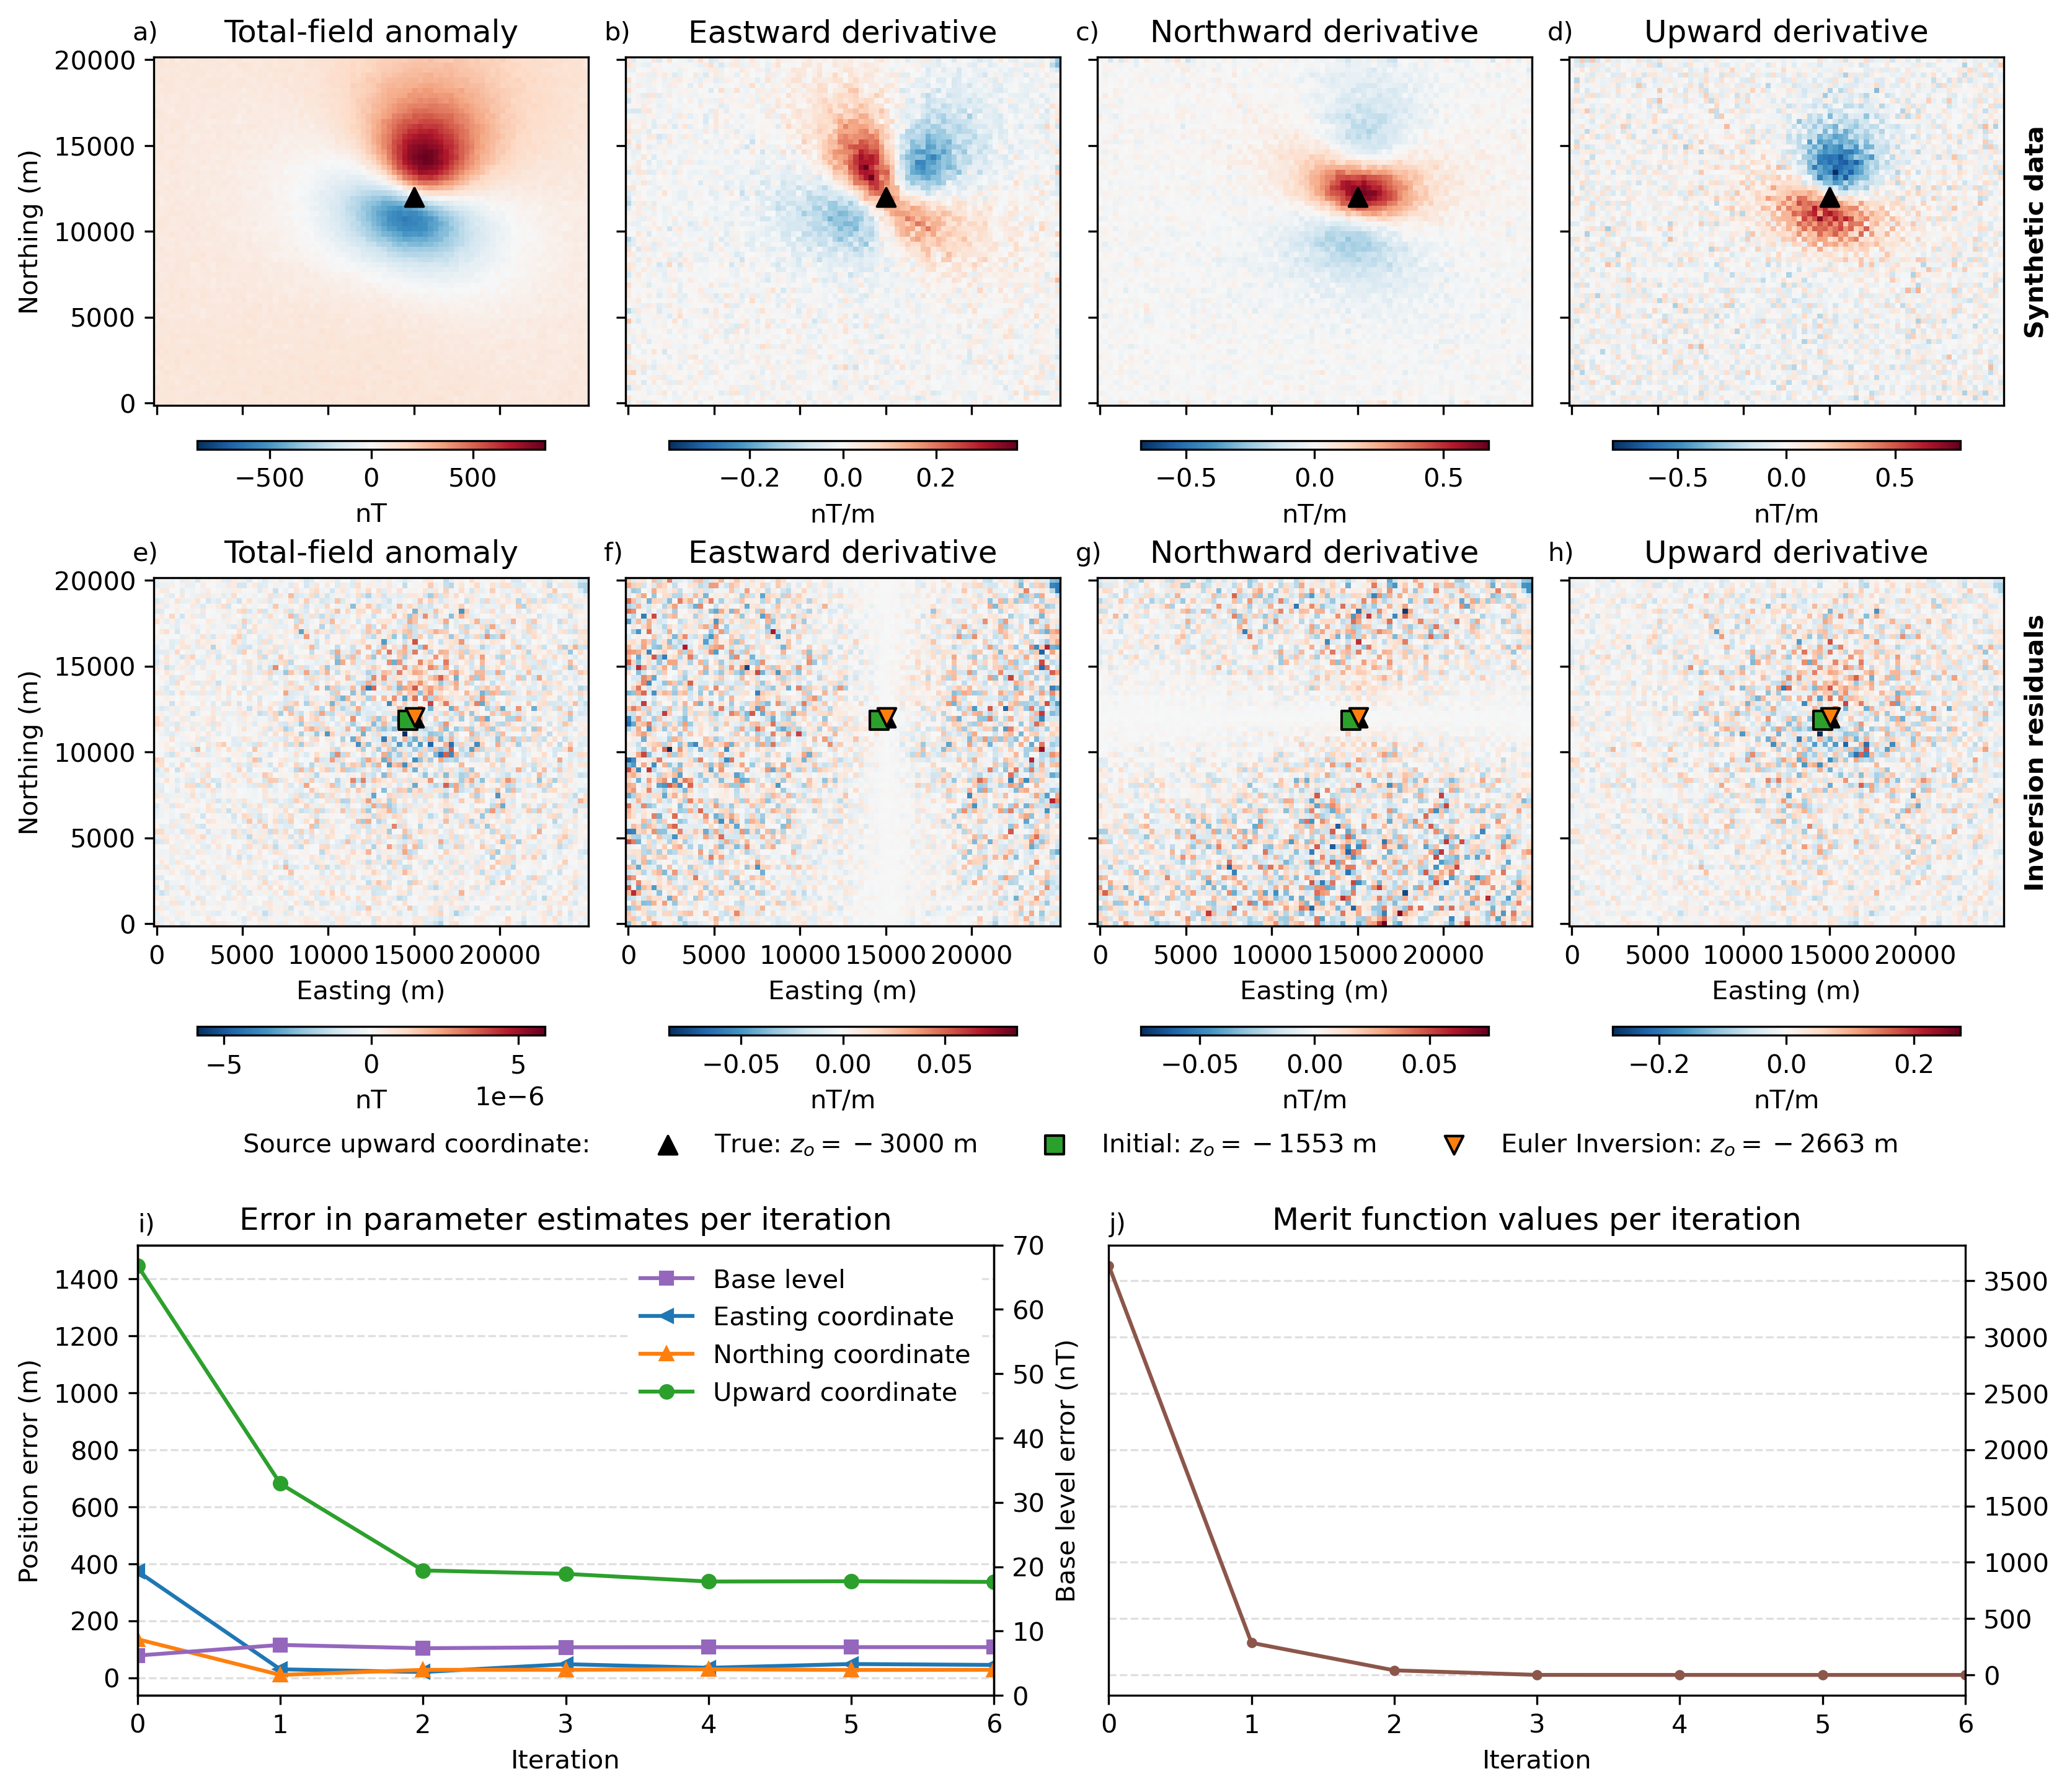
\includegraphics[width=1\linewidth]{euler-inversion/figures/synthetic-proof-of-concept.png}
\caption{
    Data and results from the synthetic data test to demonstrate the performance of the method on a single target.
    a-d) The noise-corrupted synthetic total-field anomaly and its eastward, northward, and upward derivatives, respectively. The position of the dipolar source is marked by the black triangle.
    e-h) The Euler inversion residuals (observed data minus predicted data) for the total-field anomaly and its easting, northing, and upward derivatives, respectively. The black triangle shows the true location of the source, the green square shows the location estimated by Euler deconvolution, and the orange triangle shows the location estimated by Euler inversion.
    i) The error in the estimate of the easting (blue line), northing (orange line), and upward (green line) coordinates of the source and the base level (purple line) as a function of the Gauss-Newton iteration (Algorithm~\ref{alg:ei}).
    j) The value of the merit function $\Merit$ (Equation~\ref{eq:merit}) per Gauss-Newton iteration.
}
\label{fig:proof}
\end{figure}

The main goal of this synthetic data test is to demonstrate the general effectiveness of the Euler inversion method to estimate the position and base level of a single source.
To this end, we created a model composed of a single dipole located at
$(x_o = \SynProofTrueEast, y_o = \SynProofTrueNorth, z_o = \SynProofTrueUp)$
with a dipole moment magnitude of \SynProofInt{}, inclination of \SynProofInc{}, and declination of \SynProofDec{}.
The reference field direction was the same as the dipole moment direction.
The synthetic total-field magnetic anomaly data was calculated on a regular grid
with point spacing of \SynProofSpacing{} at a height of \SynProofHeight{}.
To the data, we added a base level of \SynProofTrueBase{} and
pseudo-random Gaussian noise with \qty{0}{\nano\tesla} mean and \SynProofNoise{} standard deviation.
The eastward and northward derivatives of the total-field anomaly grid were calculated with a central-difference scheme.
The upward derivative was calculated by Fast Fourier Transform (FFT).
The synthetic anomaly and its three derivatives are shown in Figures~\ref{fig:proof}a-d.

The Euler inversion method described in Algorithm~\ref{alg:ei} was applied to the synthetic data.
We chose a fixed structural index of $\eta=3$, which is the correct index for a magnetic dipole.
For data weights, we used \DefaultWeightsF{} for the total-field anomaly, \DefaultWeightsE{} for the east-derivative, \DefaultWeightsN{} for the north-derivative, and \DefaultWeightsU{} for the upward-derivative.
These weights were chosen to counteract the increased effect of noise on the derivatives, particularly the upward derivative which was calculated through FFT.
Figures~\ref{fig:proof}e-h show the inversion residuals after convergence was achieved ($L=\SynProofNIter{}$ iterations) for the total-field anomaly and its eastward, northward, and upward derivatives, respectively.
Also shown are the true source location, the initial source location, and the predicted source location from Euler inversion.
The initial estimate of the source location was $(x_o=\SynProofEDEast,
y_o=\SynProofEDNorth, z_o=\SynProofEDUp)$ and the base level was $b
= \SynProofEDBase$, which are the Euler deconvolution results.
The final Euler inversion prediction of the source location was
$(x_o=\SynProofEstEast, y_o=\SynProofEstNorth, z_o=\SynProofEstUp)$ and the
estimated base level was $b = \SynProofEstBase$, which is an improvement on the
estimated values by Euler deconvolution (Figure~\ref{fig:proof}i).

Figure~\ref{fig:proof}i shows the error in the estimated source coordinates and base level.
We can see from the figure that the error in the $x_o$ (easting) and $y_o$
(northing) coordinates, as well as the base level, do not vary greatly from the
initial solution at iteration 0.
However, the error in the $z_o$ (upward) coordinate drops from over \qty{1400}{\m} to less than \qty{400}{\m} in two iterations.
The merit function (Equation~\ref{eq:merit}) also drops sharply in value by two iterations, as can be seen in Figure~\ref{fig:proof}j, confirming the rapid convergence of the Euler inversion method.


\subsection{Effect of structural index choice}
\label{sec:si}

\begin{figure}[tb!]
\centering
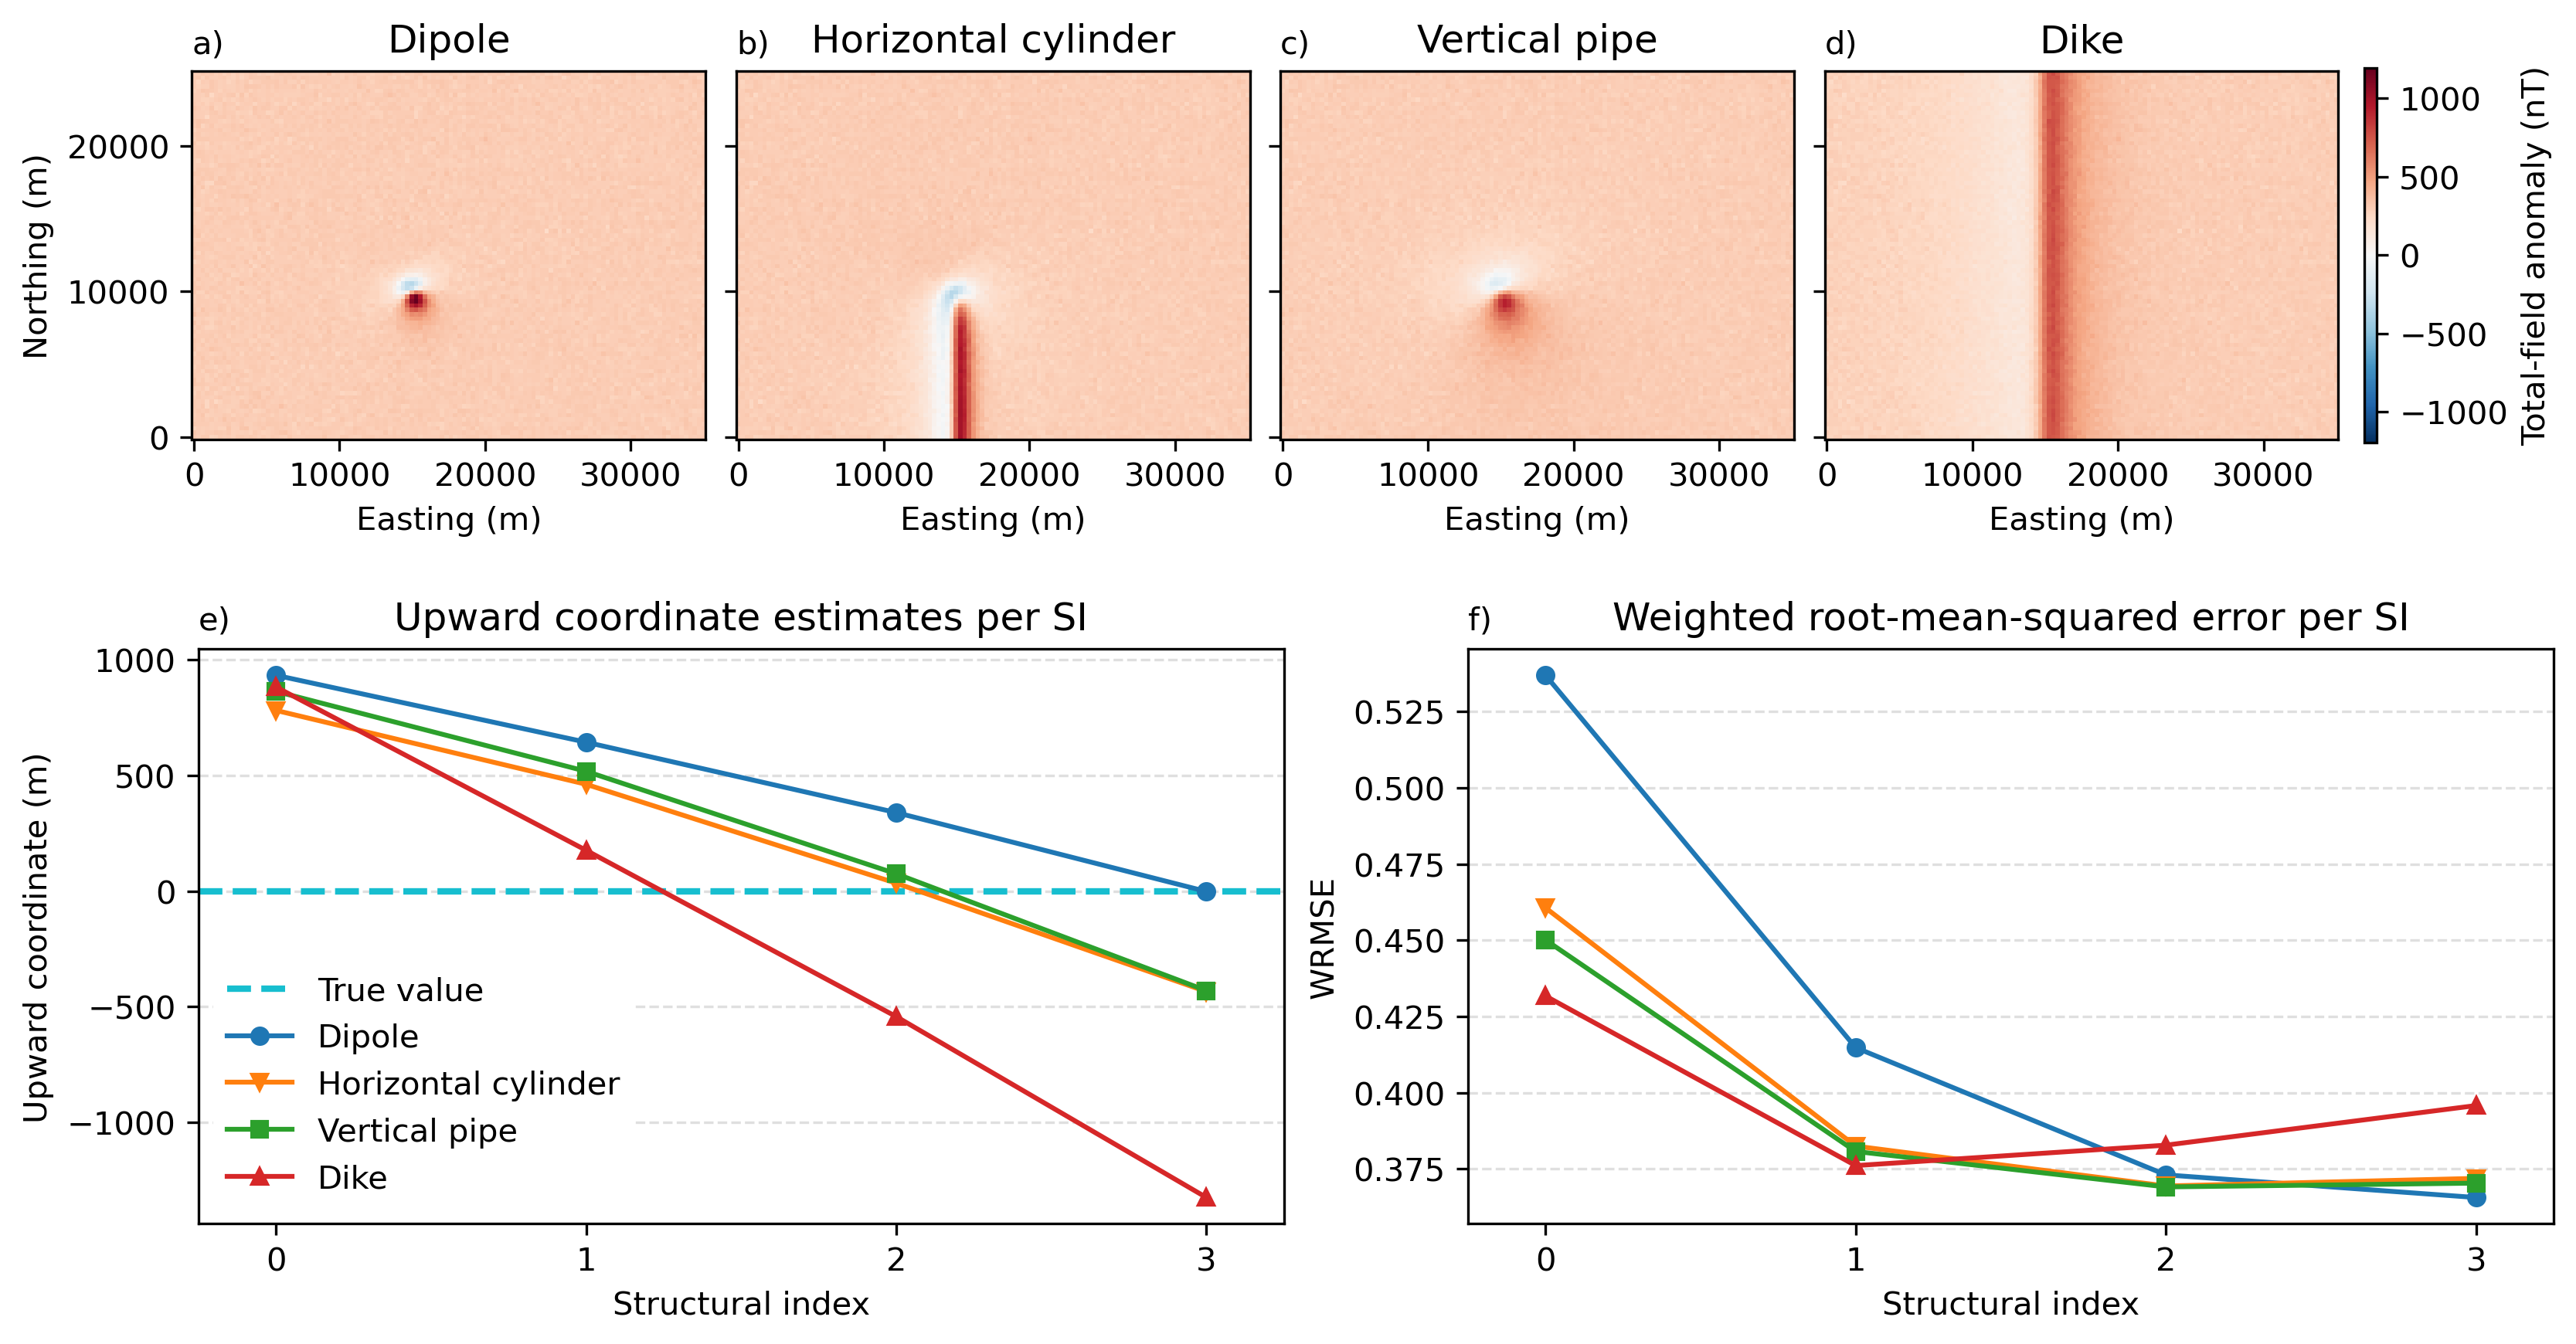
\includegraphics[width=1\linewidth]{euler-inversion/figures/synthetic-structural-index.png}
\caption{
    Data and results from the synthetic data test using different values of structural index $\eta$ for different source types.
    a-d) Noise-corrupted total-field magnetic anomaly data caused by a dipole ($\eta=3$), a horizontal cylinder ($\eta=2$), a vertical pipe ($\eta=2$), and a vertical North-South dyke ($\eta=1$), respectively.
    e) Estimate of the upward source coordinate $z_o$ as a function of structural index for the dipole (blue line), horizontal cylinder (orange line), vertical pipe (green line), and dyke (red line).
    The true upward coordinate of the sources ($z_o = \SynSITrueUp$) is marked by the blue dashed line. Note that the $z_o$ estimate is closest to the true value when the correct structural index for each source type is used.
    f) The weighted root-mean-squared error (WRMSE; Equation~\ref{eq:wrmse}) as a function of structural index for the dipole (blue line), horizontal cylinder (orange line), vertical pipe (green line), and dyke (red line). The WRMSE is minimum for each source type when the correct structural index is used.
}
\label{fig:si}
\end{figure}

In this synthetic data test, we created datasets using four different models: a dipole, a horizontal cylinder composed of a right-rectangular prism stretched in the southward direction, a vertical pipe composed of a right-rectangular prism stretched in the downward direction, and a vertical dyke composed of a right-rectangular prism stretched in the southward, northward, and downward directions.
All models share the same true location of $(x_o=\SynSITrueEast, y_o=\SynSITrueNorth, z_o=\SynSITrueUp)$, base level of \SynSITrueBase, and induced magnetisation with inclination of \SynSIInc{} and declination of \SynSIDec.
The data were generated on a regular grid with spacing of \SynSISpacing, height of \SynSIHeight, and contaminated with pseudo-random Gaussian noise with \qty{0}{\nano\tesla} mean and \SynSINoise{} standard deviation. Figures~\ref{fig:si}a-d show the synthetic noise-corrupted total-field anomaly data.

We ran the Euler inversion method on each data grid four times, each time
changing the structural index between zero, one, two, and three.
Figure~\ref{fig:si}e shows the upward coordinate $z_o$ estimated for each of the four models as a function of the structural index $\eta$.
The Euler inversion estimated $z_o$ correlates with $\eta$, with larger values of the structural index leading to deeper source estimates.
Values closest to the true $z_o=\SynSITrueUp$ are achieved when the correct structural index is used ($\eta=1$ for the dyke, $\eta=2$ for the cylinder and pipe, and $\eta=3$ for the dipole).
Figure~\ref{fig:si}f shows the weighted root-mean-squared error (WRMSE; Equation~\ref{eq:wrmse}) at the final iteration of the Euler inversion method for all four models as a function of structural index.
The WRMSE is a measure of goodness-of-fit between the predicted total-field anomaly and its three derivatives and their observed counterparts.
The WRMSE is minimum for all four models when the correct structural index is used.


\subsection{Effect of random noise}
\label{sec:noise}

\begin{figure}[tb!]
\centering
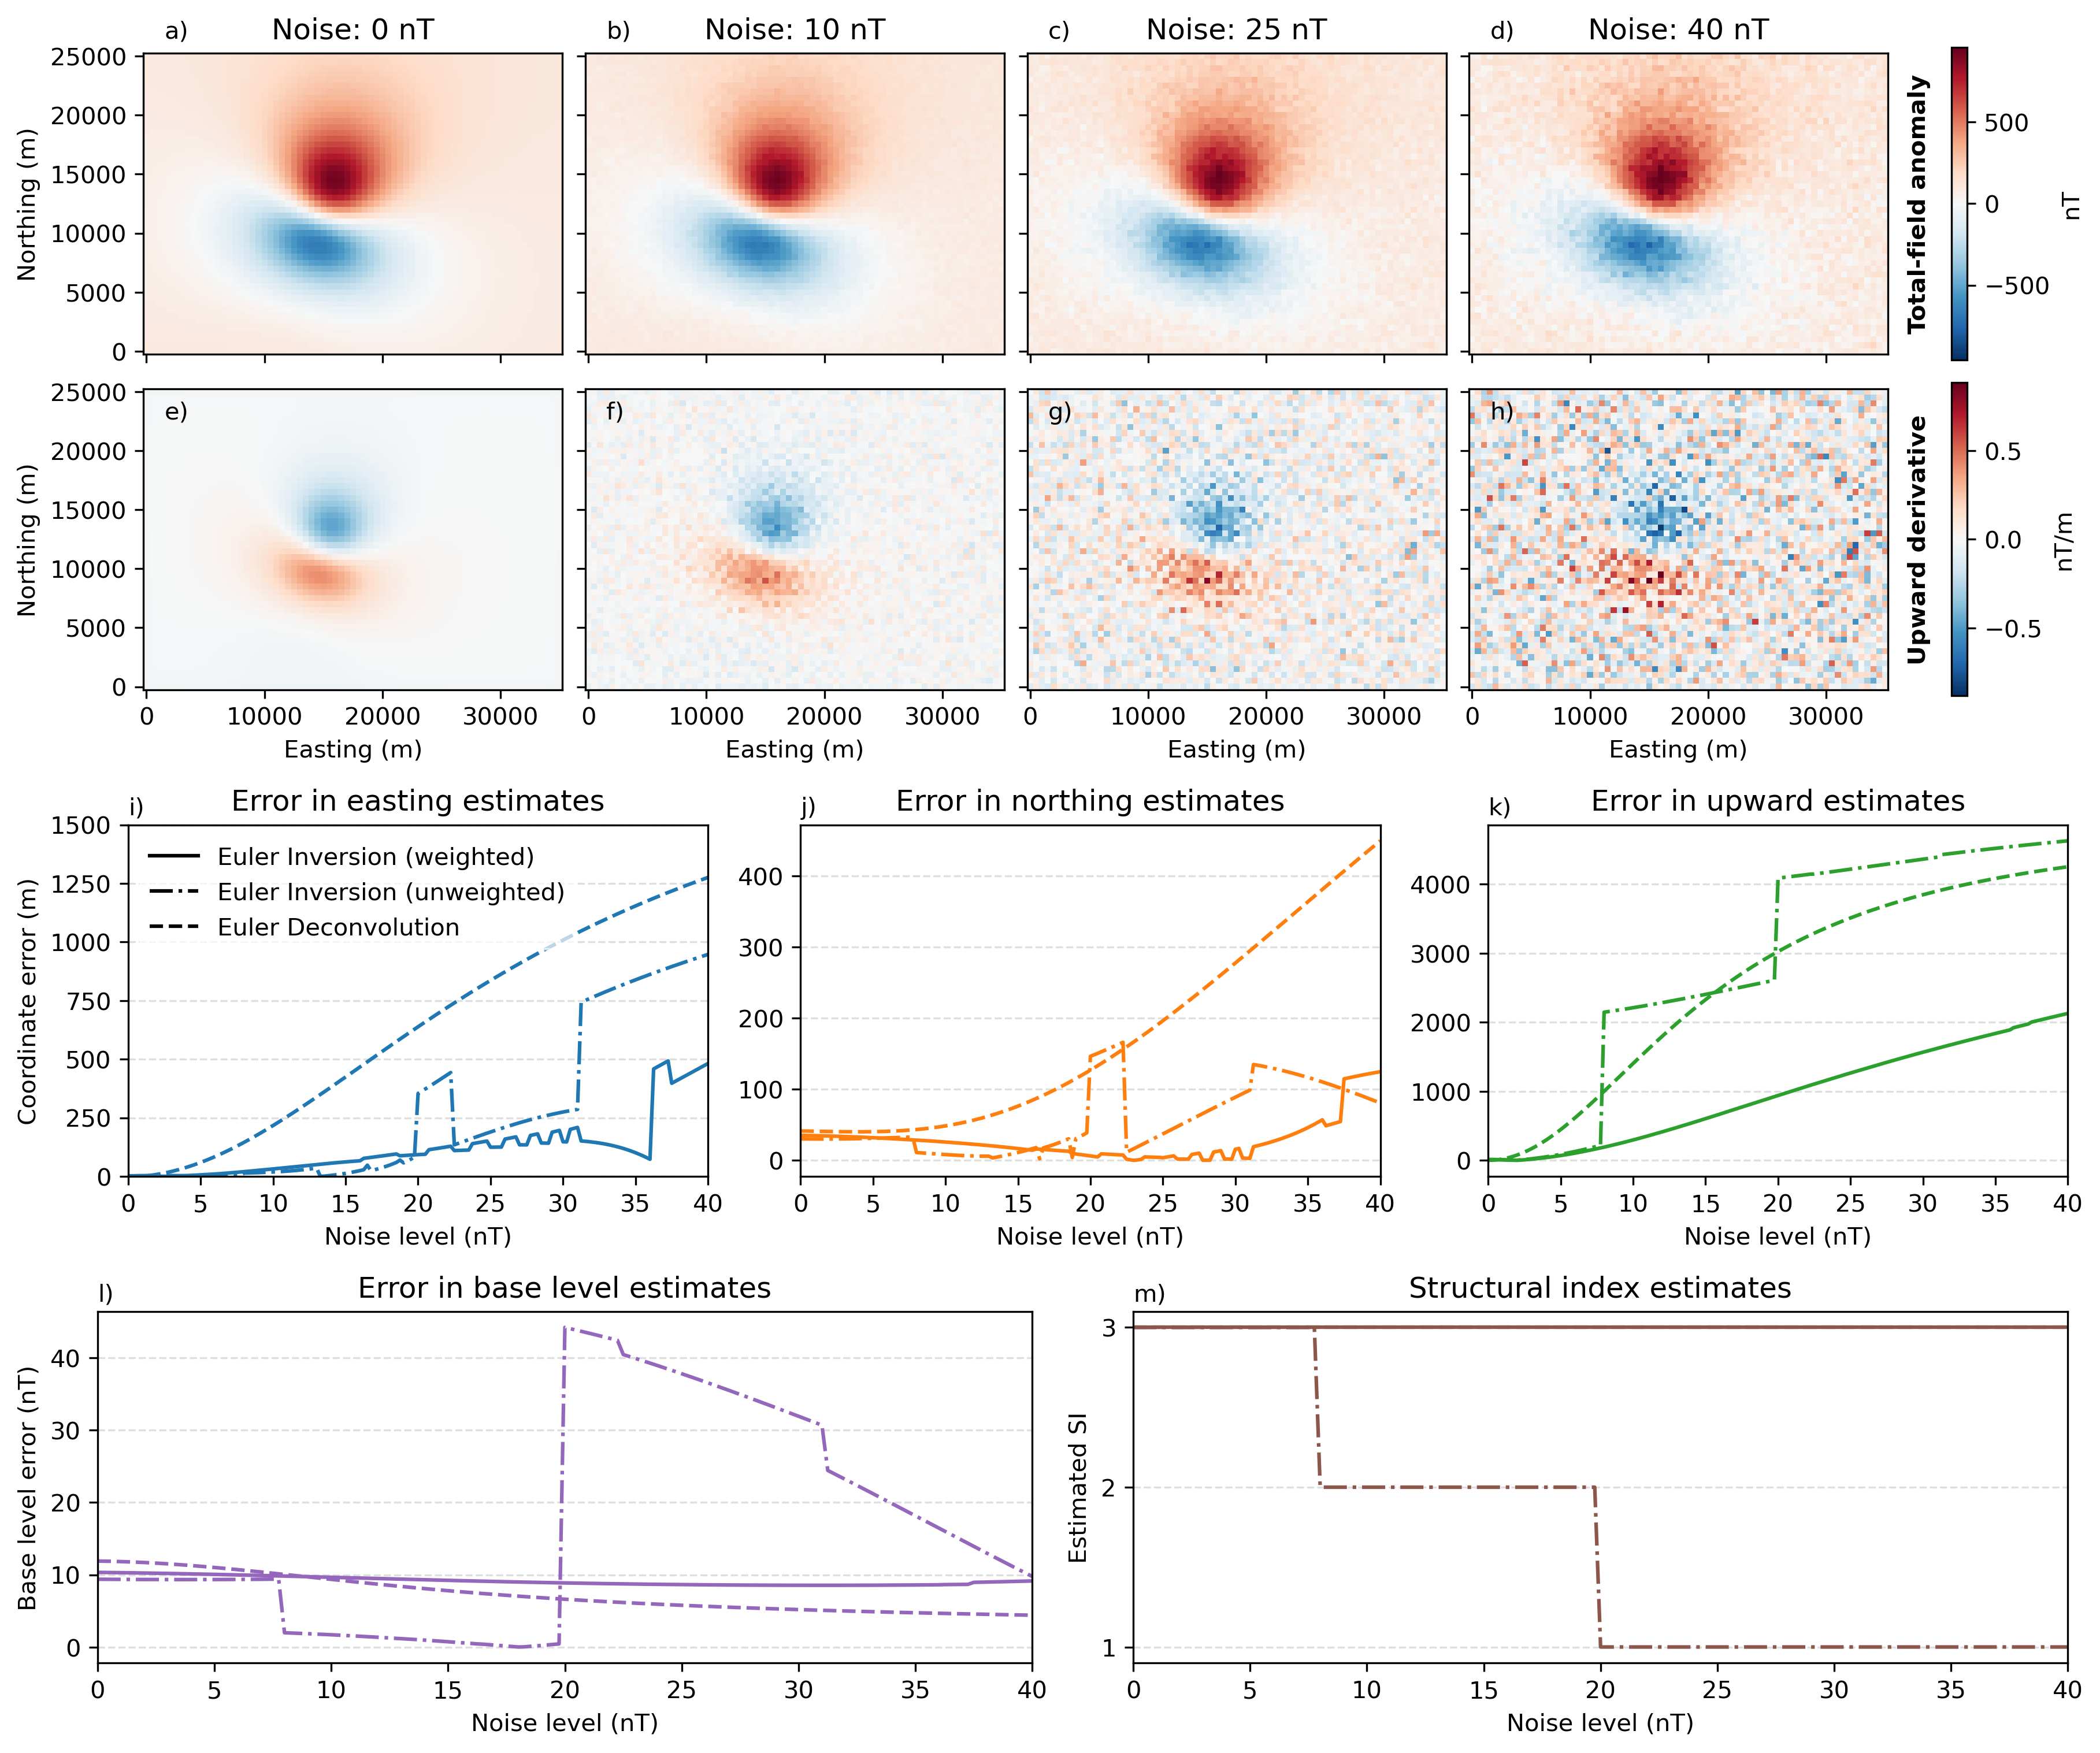
\includegraphics[width=1\linewidth]{euler-inversion/figures/synthetic-noise-levels.png}
\caption{
    Data and results from the synthetic data test used to investigate the effect of high-frequency noise on the Euler inversion results.
    a-d) Noise-corrupted total-field magnetic anomaly of a dipolar source for noise levels \SynNoisePlotted.
    e-h) The upward derivative of the data in a-d, calculated by FFT.
    i-k) Error in the estimated easting, northing, and upward coordinates, respectively.
    l) Error in the estimated base level.
    m) The estimated structural index $\eta$ using Algorithm~\ref{alg:si}.
    The lines in i-m are the results for Euler deconvolution (dashed line), Euler inversion without data weights (dashed-dotted line), and Euler inversion with weights (solid line) \SynNoiseWeightsF{} for the total-field anomaly, \SynNoiseWeightsE{} for the eastward derivative, \SynNoiseWeightsN{} for the northward derivative, and \SynNoiseWeightsU{} for the upward derivative.
}
\label{fig:noise}
\end{figure}

We conducted another experiment to determine the effect of random high-frequency noise on the Euler inversion estimates.
To this end, we created synthetic data from a dipole model located at $(x_o=\SynNoiseTrueEast, y_o=\SynNoiseTrueNorth, z_o=\SynNoiseTrueUp)$ and with a dipole moment magnitude of \SynNoiseInt{}, inclination of \SynNoiseInc, and declination of \SynNoiseDec.
The total-field anomaly data were generated on a regular grid with a spacing of \SynNoiseSpacing{} and a constant height of \SynNoiseHeight.
The reference field direction was the same as the dipole moment direction.
A base level of \SynNoiseTrueBase{} was added to the data.
We generated different datasets by adding pseudo-random Gaussian noise with \qty{0}{\nano\tesla} mean and standard deviations varying from \SynNoiseMin{} to \SynNoiseMax{} with a step of \SynNoiseStep{}.
Figures~\ref{fig:noise}a-d show the synthetic data for noise levels \SynNoisePlotted, while Figures~\ref{fig:noise}e-h show the upward derivative calculated from the total-field anomaly through FFT.

On each dataset, we ran Euler deconvolution (Equation~\ref{eq:deconv-p}), Euler inversion with unit weights, and Euler inversion with weights \SynNoiseWeightsF{} for the total-field anomaly, \SynNoiseWeightsE{} for the eastward derivative, \SynNoiseWeightsN{} for the northward derivative, and \SynNoiseWeightsU{} for the upward derivative.
Both Euler inversion runs used the structural index estimation procedure
(Algorithm~\ref{alg:si} with $\eta_{min}=\DefaultSIMin$ and
$\eta_{max}=\DefaultSIMax$).
Figures~\ref{fig:si}i-l show the error in the estimated easting, northing, and upward coordinates as well as the base level for each of the methods as a function of noise level.
The error in each of three coordinates raises sharply with noise level for Euler deconvolution, particularly for the upward $z_o$ coordinate.
The unweighted Euler inversion results vary less regularly but the present errors are just as large as Euler deconvolution for the upward coordinate.
However, the weighted Euler inversion presented overall smaller errors and a slower growth curve for the upward coordinate error than the other two methods.
The base level error is nearly constant at approximately \qty{10}{\nano\tesla} for Euler deconvolution and the weighted Euler inversion, but varies to as much as \qty{40}{\nano\tesla} for the unweighted Euler inversion.

Figure~\ref{fig:noise}m shows the estimated structural index $\eta$ for the weighted and unweighted Euler inversion as a function of noise level.
The unweighted Euler inversion estimated the wrong structural index $\eta=2$ from approximately noise level \qty{7}{\nano\tesla} and $\eta=1$ from approximately noise level \qty{20}{\nano\tesla}.
These jumps in the estimated structural index appear to correlate with jumps in the base level and $z_o$ coordinate errors.
The weighted Euler inversion was able to estimate the correct structural index ($\eta=3$) for all noise levels tested.


\subsection{Effect of interfering sources}
\label{sec:interf}

\begin{figure}[tb!]
\centering
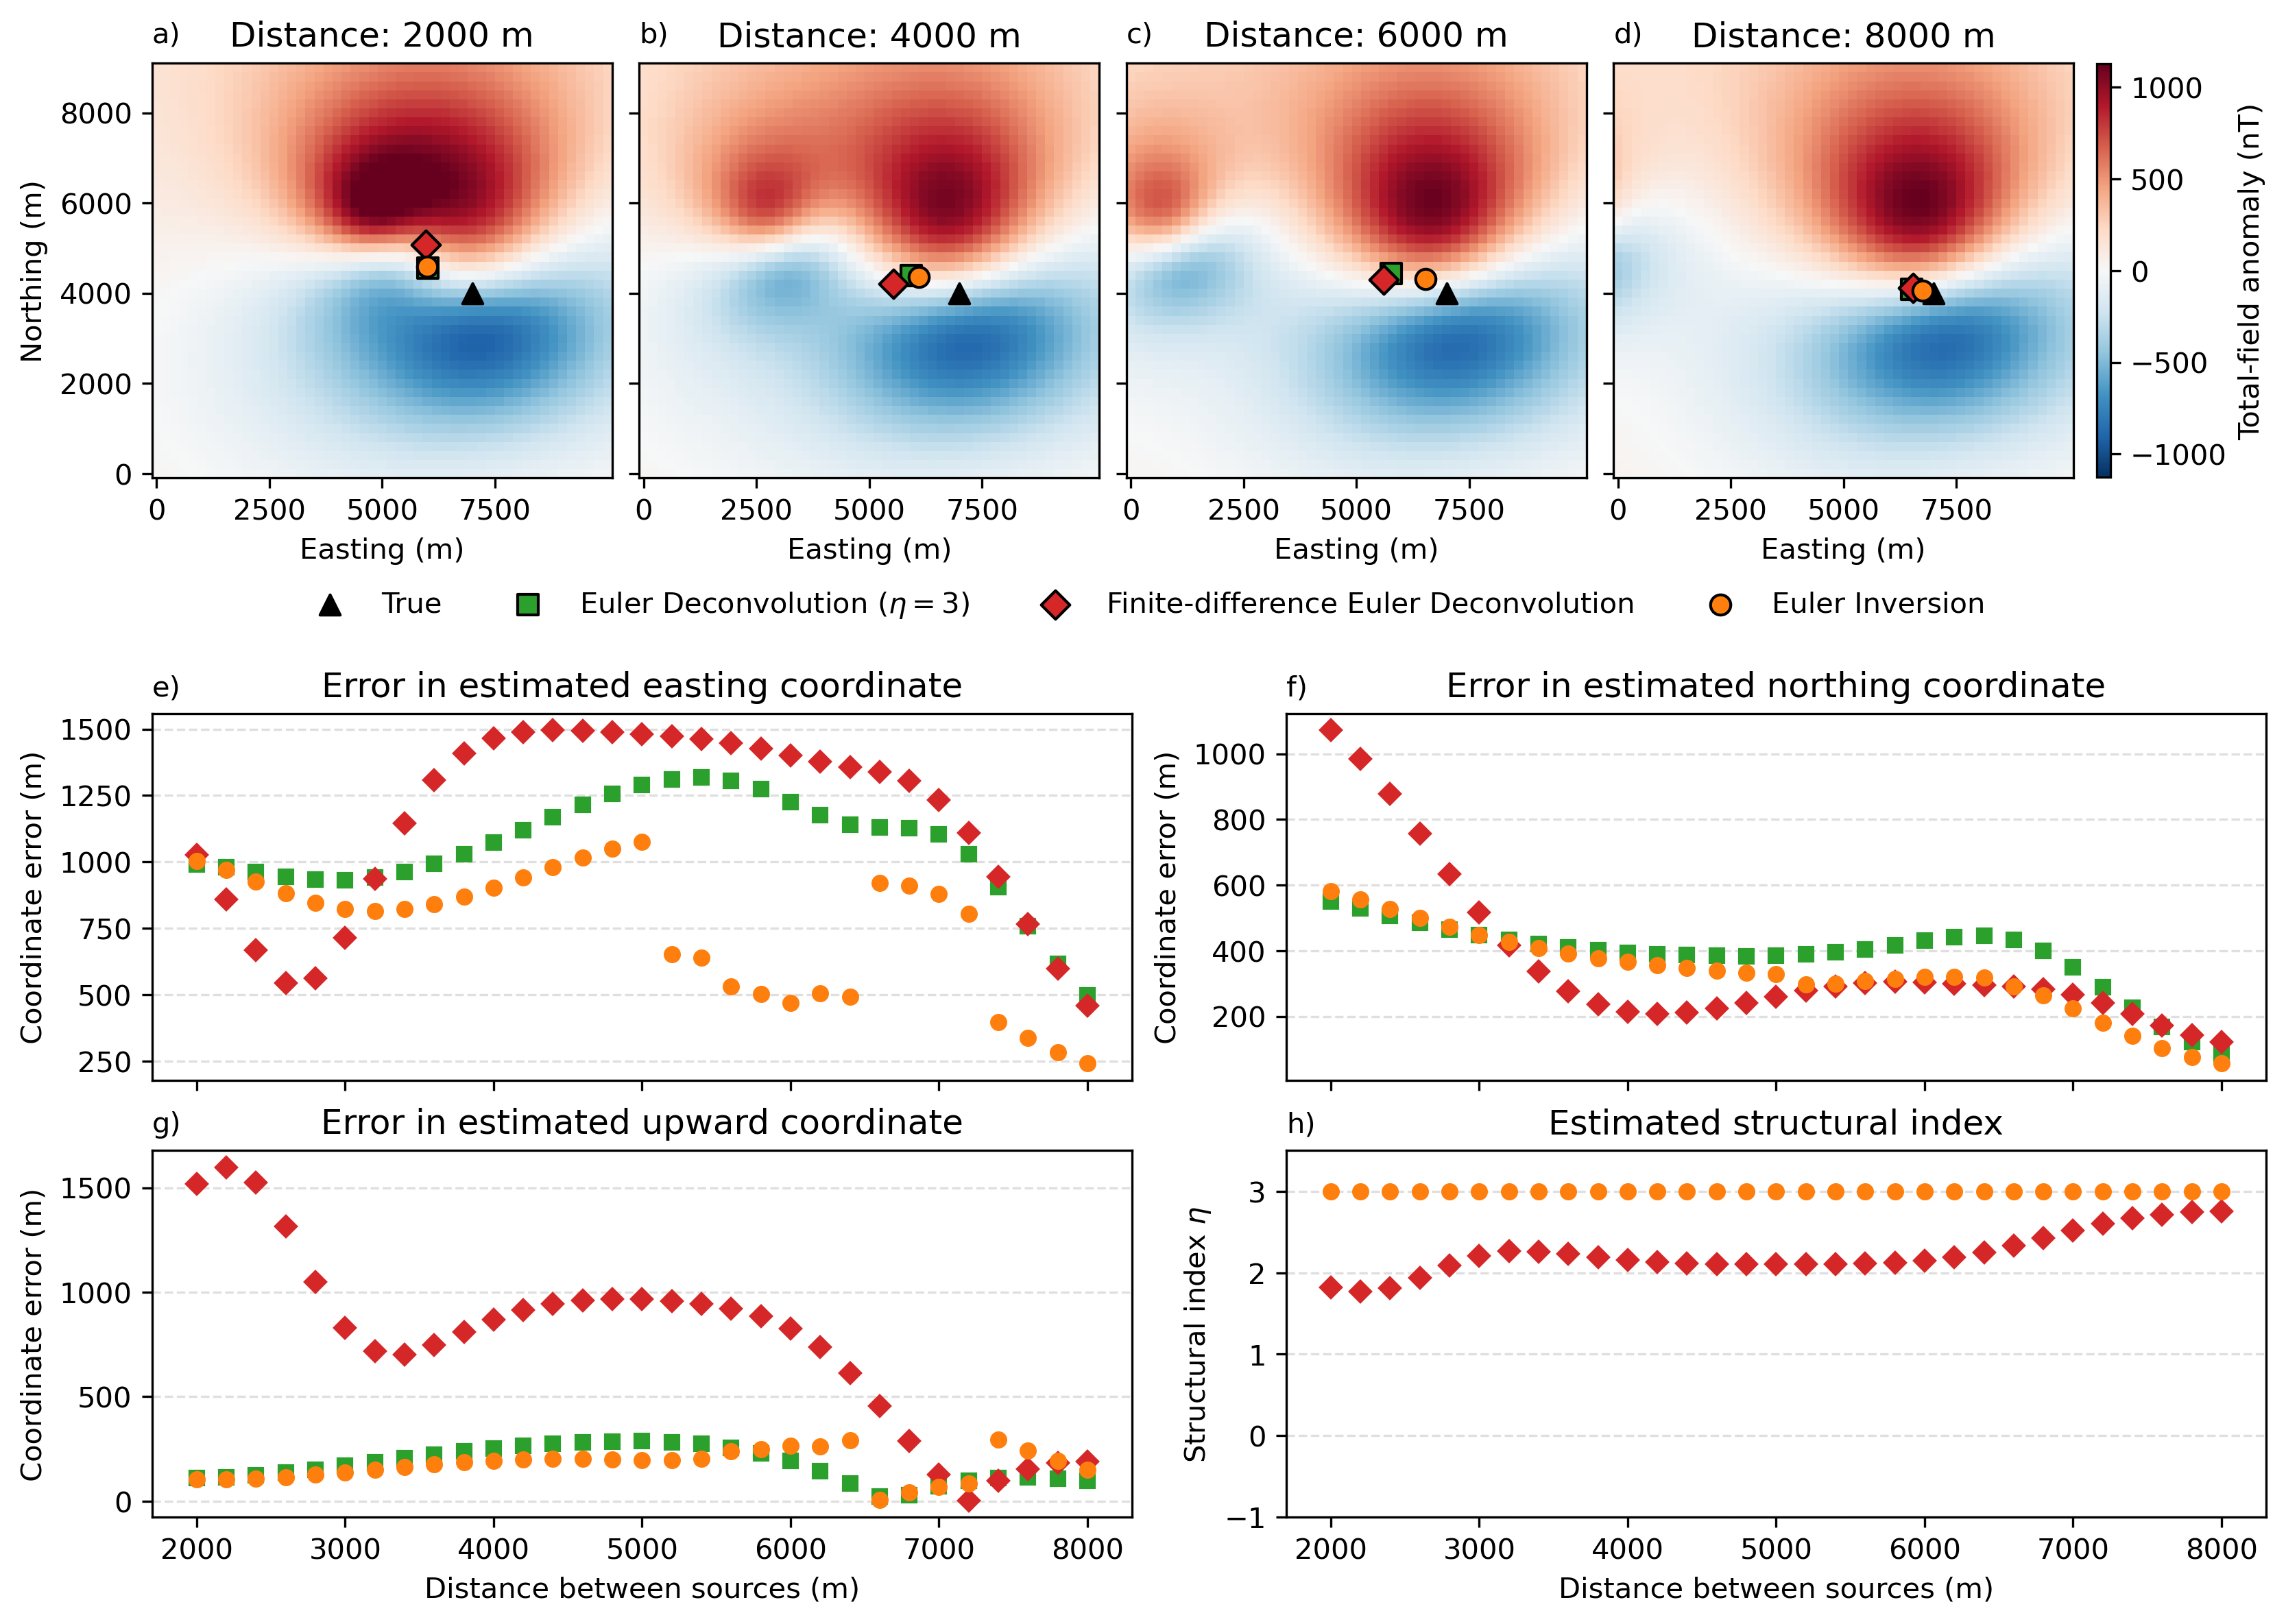
\includegraphics[width=1\linewidth]{euler-inversion/figures/synthetic-interfering-sources.png}
\caption{
    Data and results from the synthetic data test used to investigate the
    effect of interfering dipolar sources inside the data window on the Euler
    inversion results.
    a-d) Total-field magnetic anomaly of four out of the \SynInterfNModels{}
    models, each of which includes the same central dipole and an interfering
    dipolar source at different distances from the main source. Also plotted
    are the estimated positions from Euler deconvolution (green square),
    finite-difference Euler deconvolution (red diamond), and Euler inversion
    (orange circle).
    e-g) The error in the estimated eastward, northward, and upward
    coordinates, respectively, of the source for each of the Euler methods as
    a function of the distance between sources.
    h) The estimated structural index $\eta$ for Euler inversion and
    finite-difference Euler deconvolution as a function of the distance between
    sources.
}
\label{fig:interf}
\end{figure}

\begin{figure}[tb!]
\centering
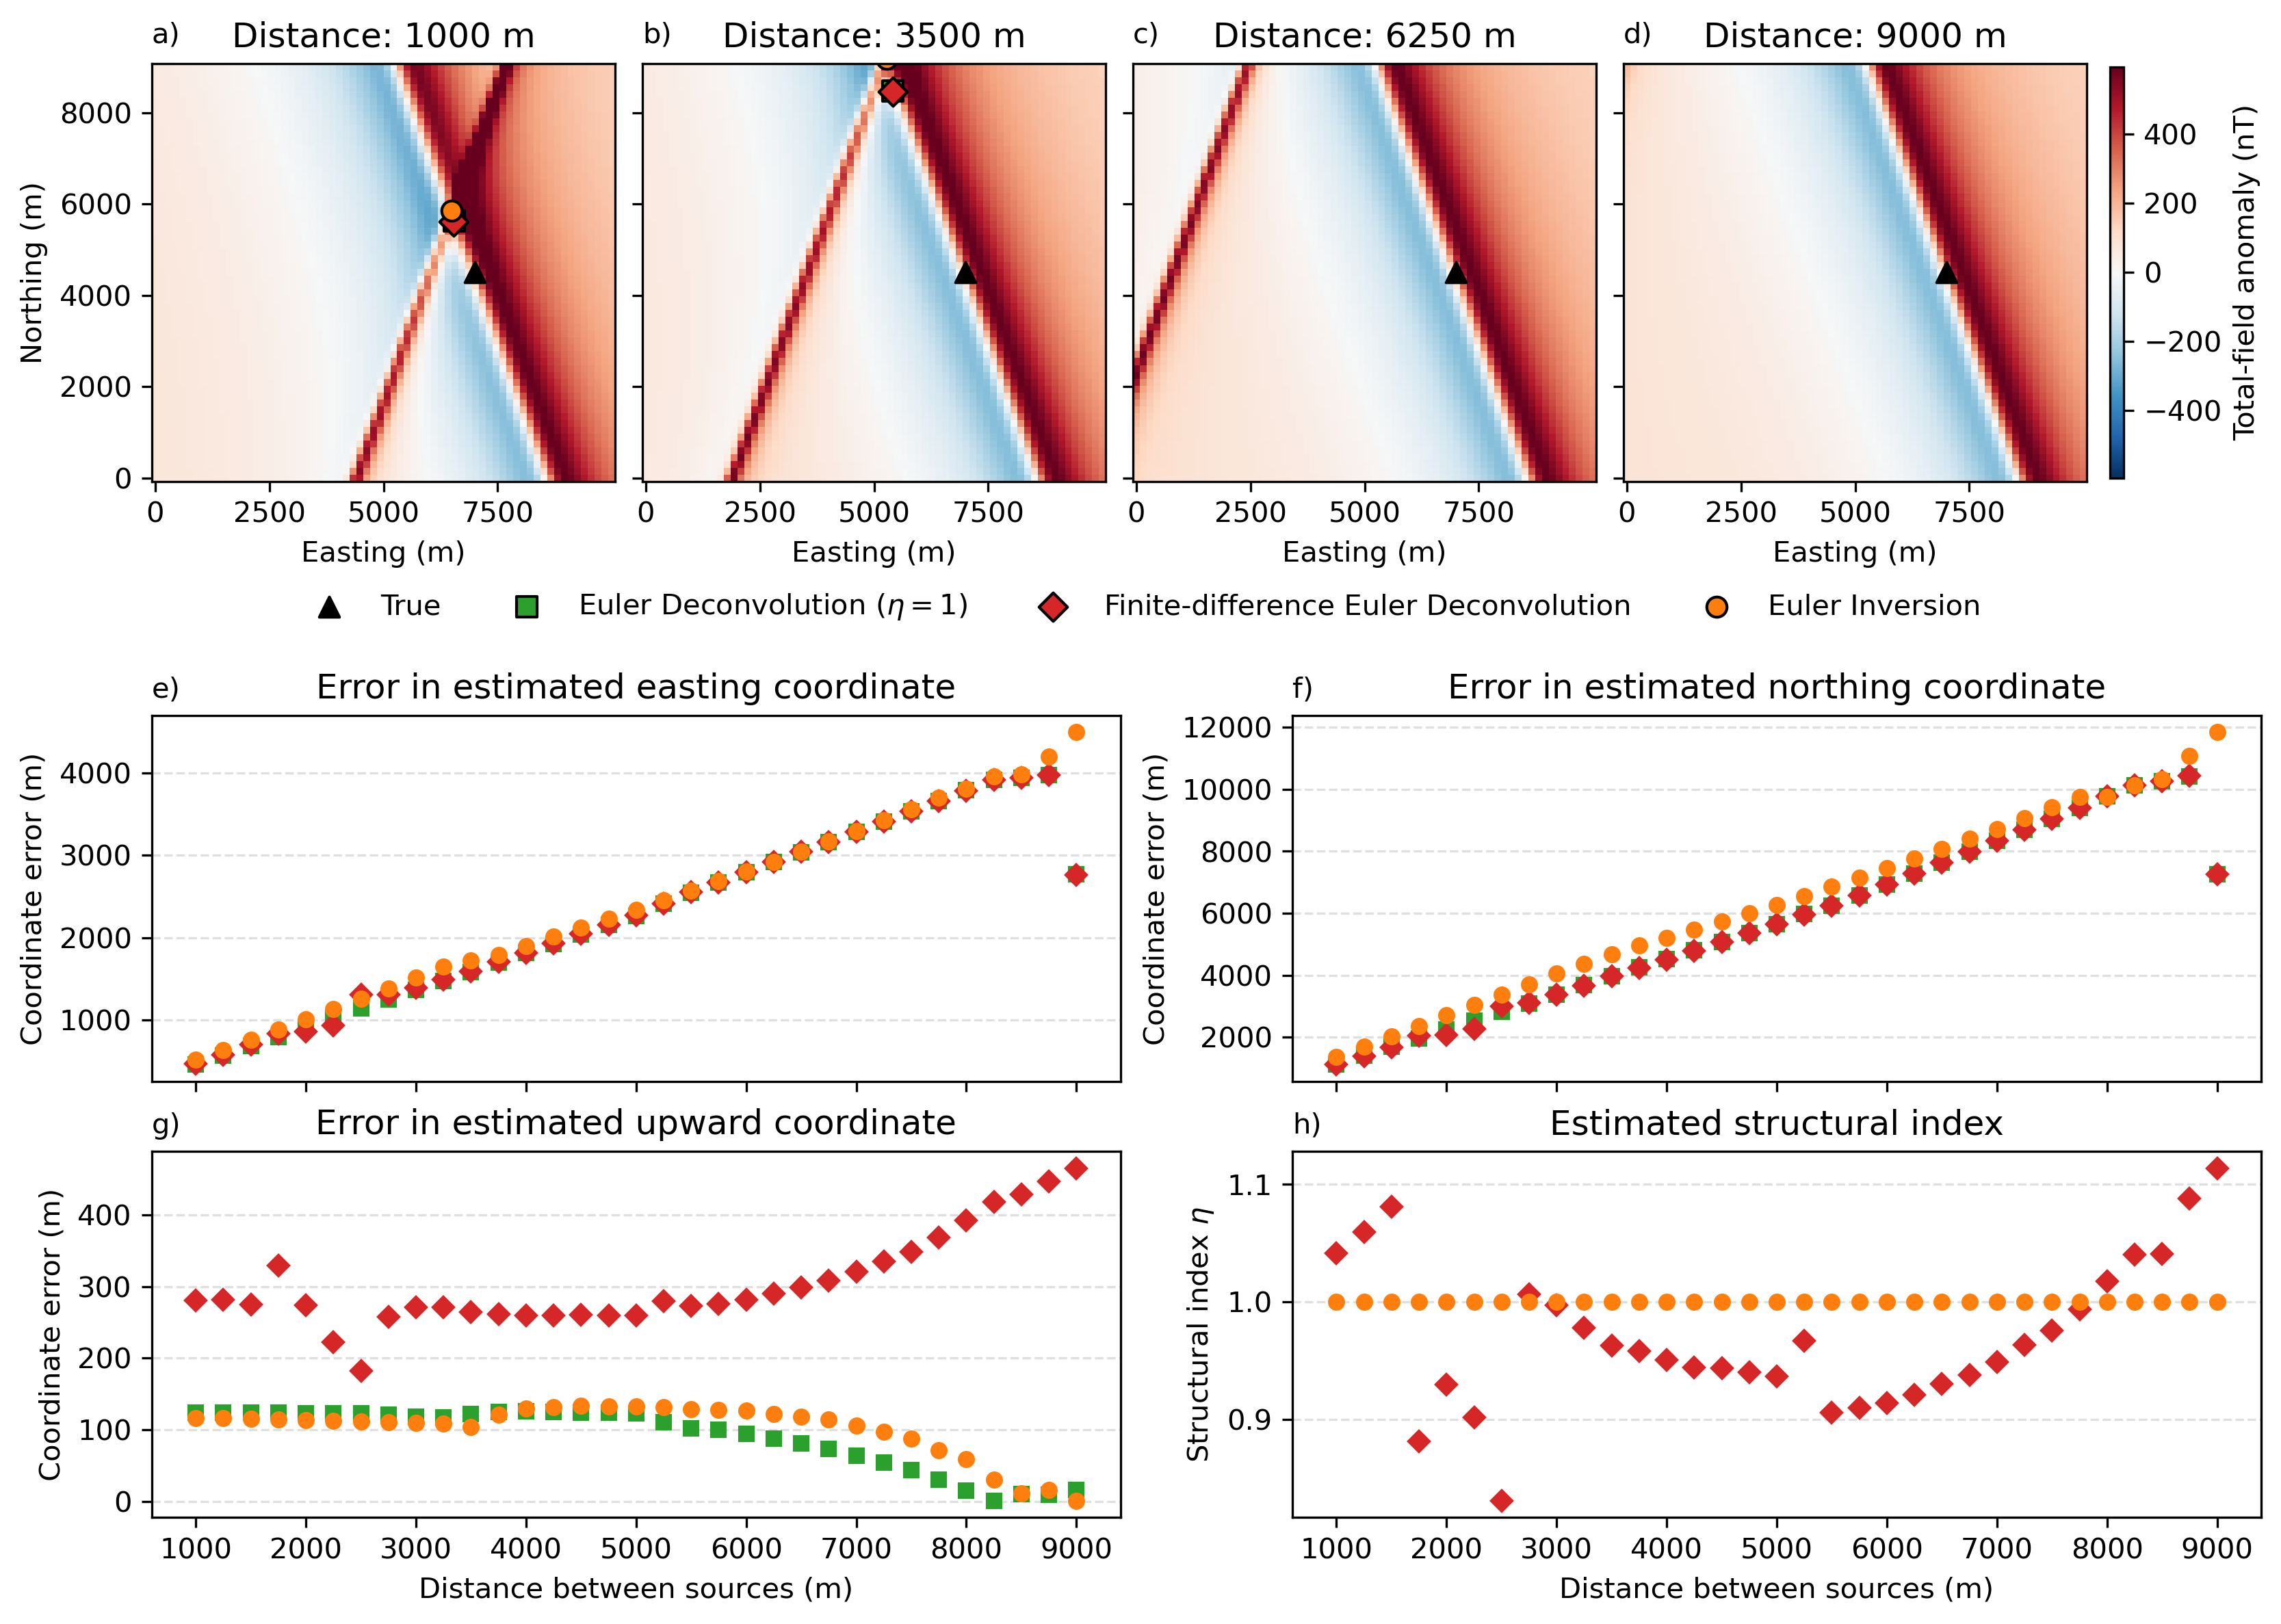
\includegraphics[width=1\linewidth]{euler-inversion/figures/synthetic-interfering-sources-dykes.png}
\caption{
    Data and results from the synthetic data test used to investigate the
    effect of interfering dykes inside the data window on the Euler inversion
    results.
    a-d) Total-field magnetic anomaly of four out of the \SynInterfDykesNModels{}
    models, each of which includes the same dyke to the east and an interfering
    dyke to the west at different distances from the main source. Also plotted
    are the estimated positions from Euler deconvolution (green square),
    finite-difference Euler deconvolution (red diamond), and Euler inversion
    (orange circle).
    In c and d, the three Euler solutions are not visible because they are
    outside the data window.
    e-g) The error in the estimated eastward, northward, and upward
    coordinates, respectively, of the source for each of the Euler methods as
    a function of the distance between sources. The error for the eastward and
    northward coordinates was calculated with respect to the center point of
    the eastern dyke (black triangle).
    h) The estimated structural index $\eta$ for Euler inversion and
    finite-difference Euler deconvolution as a function of the distance between
    sources.
}
\label{fig:interf-dykes}
\end{figure}

Another common issue encountered during the application of Euler-based methods
is the presence of interfering sources within the data window.
To test this effect on Euler inversion, we create two different scenarios, one
with two dipoles and another with two dykes.
In both scenarios, we created several synthetic total-field anomaly datasets
by varying the distance between the two sources.
No noise was added to these synthetic data in order to isolate the effect of
the interfering source from the effect of random noise.
We added to all datasets a base level of \SynInterfTrueBase{}.
On each dataset, we ran Euler deconvolution (Equation~\ref{eq:deconv-p}) with
the correct structural index for the source ($\eta=3$ for the dipoles and
$\eta=1$ for the dykes), the finite-difference Euler deconvolution method of
\citet{Gerovska2005}, and Euler inversion with the structural index estimation
(Algorithm~\ref{alg:si} with $\eta_{min}=\DefaultSIMin$ and
$\eta_{max}=\DefaultSIMax$) and data weights of \DefaultWeightsF{} for the
total-field anomaly, \DefaultWeightsE{} for the eastward derivative,
\DefaultWeightsN{} for the northward derivative, and \DefaultWeightsU{} for the
upward derivative.

The dipole models contain a main dipole located at $(x_o=\SynInterfTrueEast,
y_o=\SynInterfTrueNorth, z_o=\SynInterfTrueUp)$ with a dipole moment amplitude
of \SynInterfInt{}, inclination of \SynInterfInc, and declination of
\SynInterfDec.
The interfering dipole was located at $y_o=\SynInterfInterfNorth$ and
$z_o=\SynInterfInterfUp$, with the $x_o$ coordinate varying from
\SynInterfInterfEastMin{} to \SynInterfInterfEastMax{}.
The reference field direction was the same as the dipole moment direction.
The total-field anomaly data were generated on regular grids with a spacing of
\SynInterfSpacing{} and at a constant height of \SynInterfHeight.
Figures~\ref{fig:interf}a-d show the total-field anomaly of four out of the
\SynInterfNModels{} models.

The error in the estimated eastward, northward, and upward coordinates are
shown in Figures~\ref{fig:interf}e-g.
For the eastward and northward coordinates, the three methods are mostly
compatible, with Euler inversion being slightly closer to the true source for
most distances between sources.
For the upward coordinate, Euler inversion and Euler deconvolution are
roughly equivalent and both have smaller errors than finite-difference Euler
deconvolution for all but the largest distances.
For the structural index estimates (Figure~\ref{fig:interf}h),
finite-difference Euler deconvolution underestimates $\eta$ for all but the
largest distances, while Euler inversion estimates the correct index of
$\eta=3$ for all distances.

The dyke models contain a main dyke at the east with a center point at
$(x_o=\SynInterfDykesTrueEast, y_o=\SynInterfDykesTrueNorth)$ and a top at
$z_o=\SynInterfDykesTrueUp$ with a dipole moment amplitude
of \SynInterfDykesInt{}, inclination of \SynInterfDykesInc, and declination of
\SynInterfDykesDec.
The interfering dyke has a top at $z_o=\SynInterfDykesInterfUp$, with the $x_o$
coordinate varying from
\SynInterfDykesInterfEastMin{} to \SynInterfDykesInterfEastMax{}.
The reference field direction was the same as the dipole moment direction.
The total-field anomaly data were generated on regular grids with a spacing of
\SynInterfDykesSpacing{} and at a constant height of \SynInterfDykesHeight.
Figures~\ref{fig:interf-dykes}a-d show the total-field anomaly of four out of
the \SynInterfDykesNModels{} models.

The error in the estimated eastward, northward, and upward coordinates are
shown in Figures~\ref{fig:interf-dykes}e-g.
The error for the eastward and northward coordinates was calculated with
respect to the center point of the eastern dyke.
For the eastward and northward coordinates, the three methods are mostly
compatible.
When the two dykes intersect, all three methods estimate a horizontal position
at the intersection point.
When they don't intersect, the estimates for all three methods falls outside of
the data window.
This is a well known issue for Euler deconvolution methods because the Hessian
matrix $\mathbf{A}^T\mathbf{A}$ (Equation~\ref{eq:deconv-p}) is ill-conditioned
for 2D sources \citep{Mushayandebvu2004}.
For the upward coordinate, Euler inversion and Euler deconvolution are
roughly equivalent and approach zero at the largest distances.
Both methods have smaller errors than finite-difference Euler deconvolution for
all distances tested.
For the structural index estimates (Figure~\ref{fig:interf-dykes}h),
finite-difference Euler deconvolution estimates incorrect $\eta$ at most
distances, presenting no clear relationship between distance and $\eta$
estimate.
Euler inversion estimates the correct index of $\eta=1$ for all distances.


\subsection{Moving window procedure with multiple sources}
\label{sec:windows}

\begin{figure}[tb!]
\centering
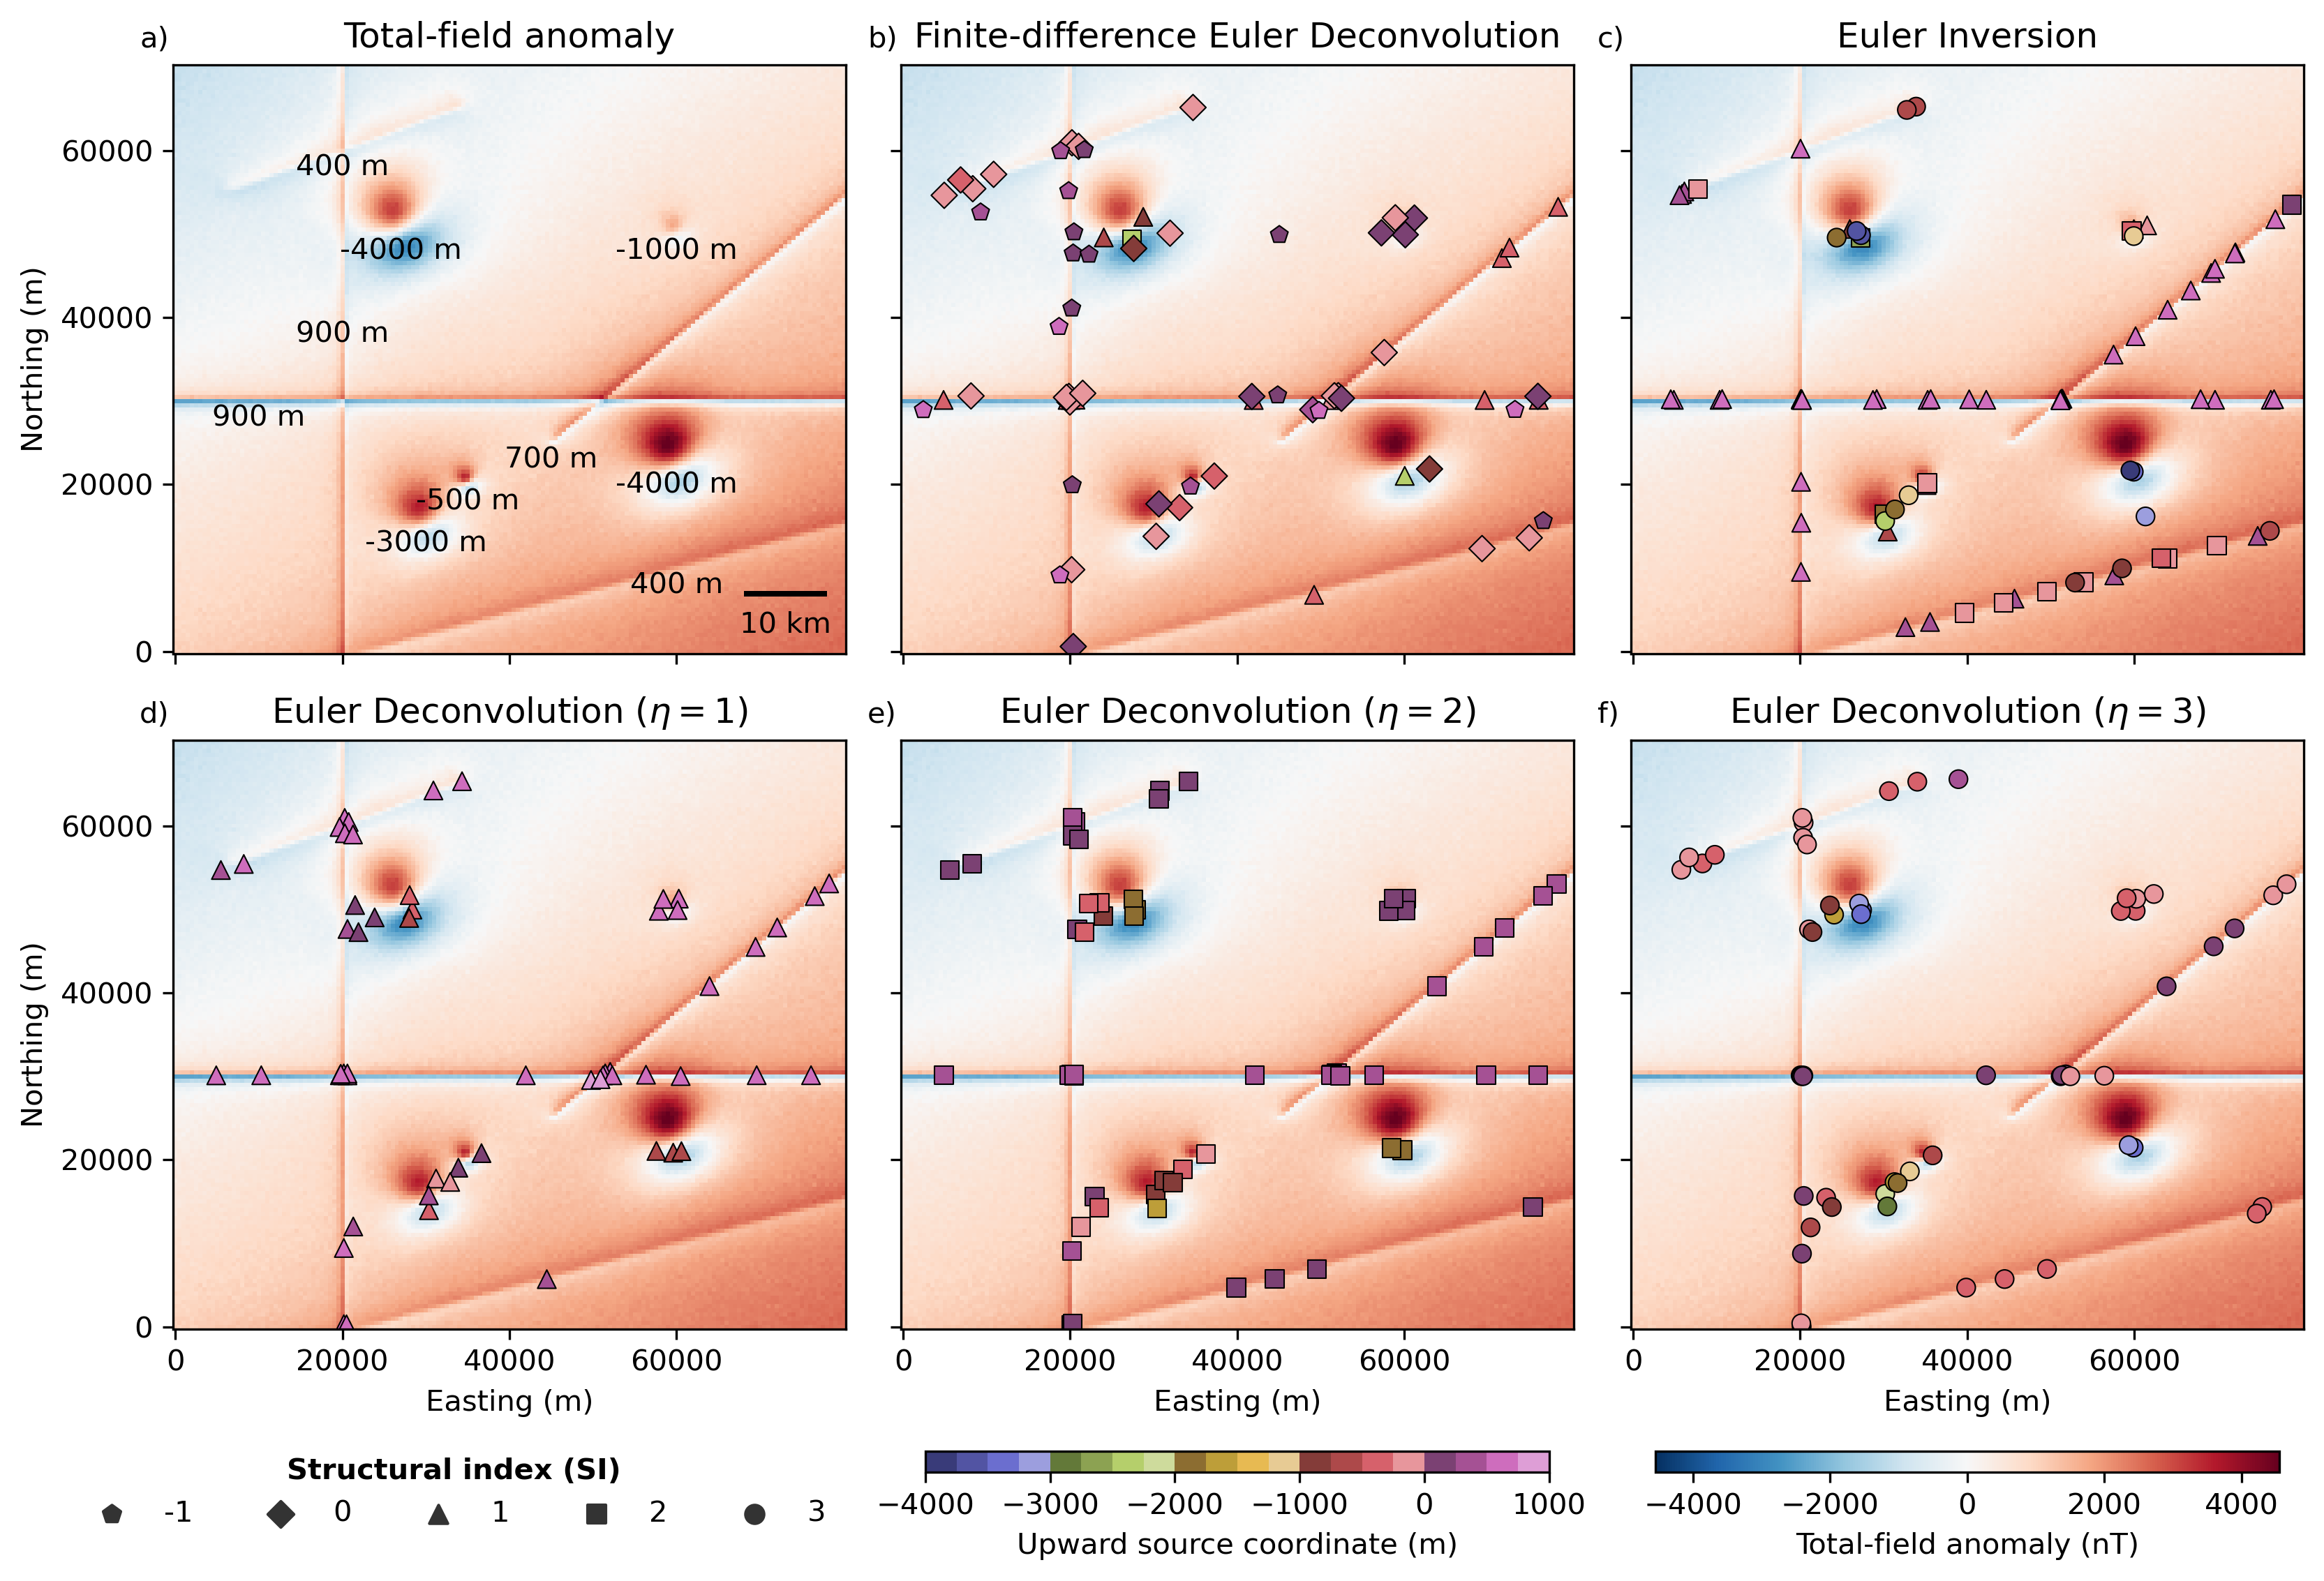
\includegraphics[width=1\linewidth]{euler-inversion/figures/synthetic-windows.png}
\caption{
    Data and results from the synthetic data test using the moving window
    scheme (Algorithm~\ref{alg:window}).
    a) Noise-corrupted total-field magnetic anomaly generated from
    \SynWinNSources{} sources with overlapping signals, including dykes and
    dipoles. The true upward coordinate $z_o$ of each source is shown next to
    their respective anomalies.
    b-f) The estimated source locations from finite-difference Euler
    deconvolution, Euler inversion, Euler deconvolution ($\eta=1$), Euler
    deconvolution ($\eta=2$), and Euler deconvolution ($\eta=3$), respectively.
    The total-field anomaly is shown in the background for reference.
    The structural index of the solutions are represented by pentagons
    ($\eta=-1$),  diamonds ($\eta=0$),  triangles ($\eta=1$),  squares
    ($\eta=2$), and circles ($\eta=3$).
    For finite-difference Euler deconvolution (b), the structural index symbol
    is that of the closest integer to the estimated value.
    The color of each symbol represents the estimated upward coordinate $z_o$.
    The window size used was \SynWinWindowSize{} and the step between windows
    was \SynWinWindowStep{}.
}
\label{fig:windows}
\end{figure}

To simulate a more realistic dataset, we created a model composed of
\SynWinNSources{} sources combining dipoles at various locations and depths and
vertical dykes at various orientations.
All sources had induced magnetisation in the direction of the regional field
with a inclination of \SynWinInc{} and declination of \SynWinDec{}.
The total-field anomaly of the model was calculated on a regular grid with
a spacing of \SynWinSpacing{} and at a constant height of \SynWinHeight{}.
We added to the data a base level of \SynWinBase{}, pseudo-random Gaussian
noise with \qty{0}{\nano\tesla} and \SynWinNoise{} standard deviation, and
a regional field composed of a first-degree polynomial with angular
coefficients of \SynWinRegionalE{} in the eastward and \SynWinRegionalN{} in
the northward directions.
The noise-corrupted total-field anomaly data are shown in
Figure~\ref{fig:windows}a.

To the dataset, we applied the moving window Euler inversion method
(Algorithm~\ref{alg:window} and Algorithm~\ref{alg:si} with
$\eta_{min}=\DefaultSIMin$ and $\eta_{max}=\DefaultSIMax$), the
finite-difference Euler deconvolution method
of \citet{Gerovska2005}, and standard Euler deconvolution (using structural
indices 1, 2, and 3).
Euler inversion was performed with data weights of \DefaultWeightsF{} for the
total-field anomaly, \DefaultWeightsE{} for the eastward derivative,
\DefaultWeightsN{} for the northward derivative, and \DefaultWeightsU{} for the
upward derivative.
All three methods used the same moving window procedure described in
Algorithm~\ref{alg:window} for the sake of comparison.
The windows had a size of \SynWinWindowSize{} and were moved by
\SynWinWindowStep{} at a time.
The ratio of estimates kept to form the final solution was
$\gamma=\SynWinKeepED$ for Euler deconvolution, $\gamma=\SynWinKeepFD$ for
finite-difference Euler deconvolution, and $\gamma=\SynWinKeepEI$ for Euler
inversion.

Figures~\ref{fig:windows}b-f show the estimated source positions and structural
indices for finite-difference Euler deconvolution, Euler inversion, and Euler
deconvolution with structural indices 1, 2, and 3, respectively.
The finite-difference method estimates a non-integer structural index, as
a result Figure~\ref{fig:windows}b shows the closest integer value to the
actual estimated $\eta$.
The finite-difference Euler deconvolution method underestimates the structural
indices of all sources and, therefore, also underestimates their depths.
The finite-difference method solutions are also more scattered than their Euler
deconvolution and Euler inversion counterparts.
The Euler deconvolution results are closer to the correct depths when the
correct structural index is used.
They present larger dispersion than Euler inversion in areas where the signals
of multiple sources overlap.
With the exception of the deeper dykes in the northwest and southeast and the
small dipole with $z_o=\qty{-500}{\m}$, Euler inversion is able to estimate the
correct structural index for most sources.
The upward coordinate estimates for Euler inversion are also closer than Euler
deconvolution to their true values when the correct structural index was
estimated.
Euler inversion notably estimates an incorrect $\eta$ and $z_o$ for smaller
sources when there is a large amount of interference in the anomalies and for
dykes that are deeper and produce a smoother signal.

It is also notable that there are solutions that outline the simulated dykes
for all three methods.
This seems to be in contradiction of the results presented in
Section~\ref{sec:interf} and the theoretical proof in
\citet{Mushayandebvu2004}, which show that the $x_o$ and $y_o$ coordinates
cannot be estimated for 2D sources.
However, these results are widely known in practice where Euler
deconvolution-based methods are routinely used to map dykes and lineaments.
We believe that this is the effect of high-frequency noise.
The derivatives, which appear in the Jacobian matrix
(Equation~\ref{eq:deconv-system}), will contain this high-frequency noise as
well which is not 2D in nature.
This in turn causes the Hessian matrix (Equation~\ref{eq:deconv-p}) to not be
singular in practice.


\subsection{Aeromagnetic data from Rio de Janeiro}
\label{sec:rio}

\begin{figure}[tb!]
\centering
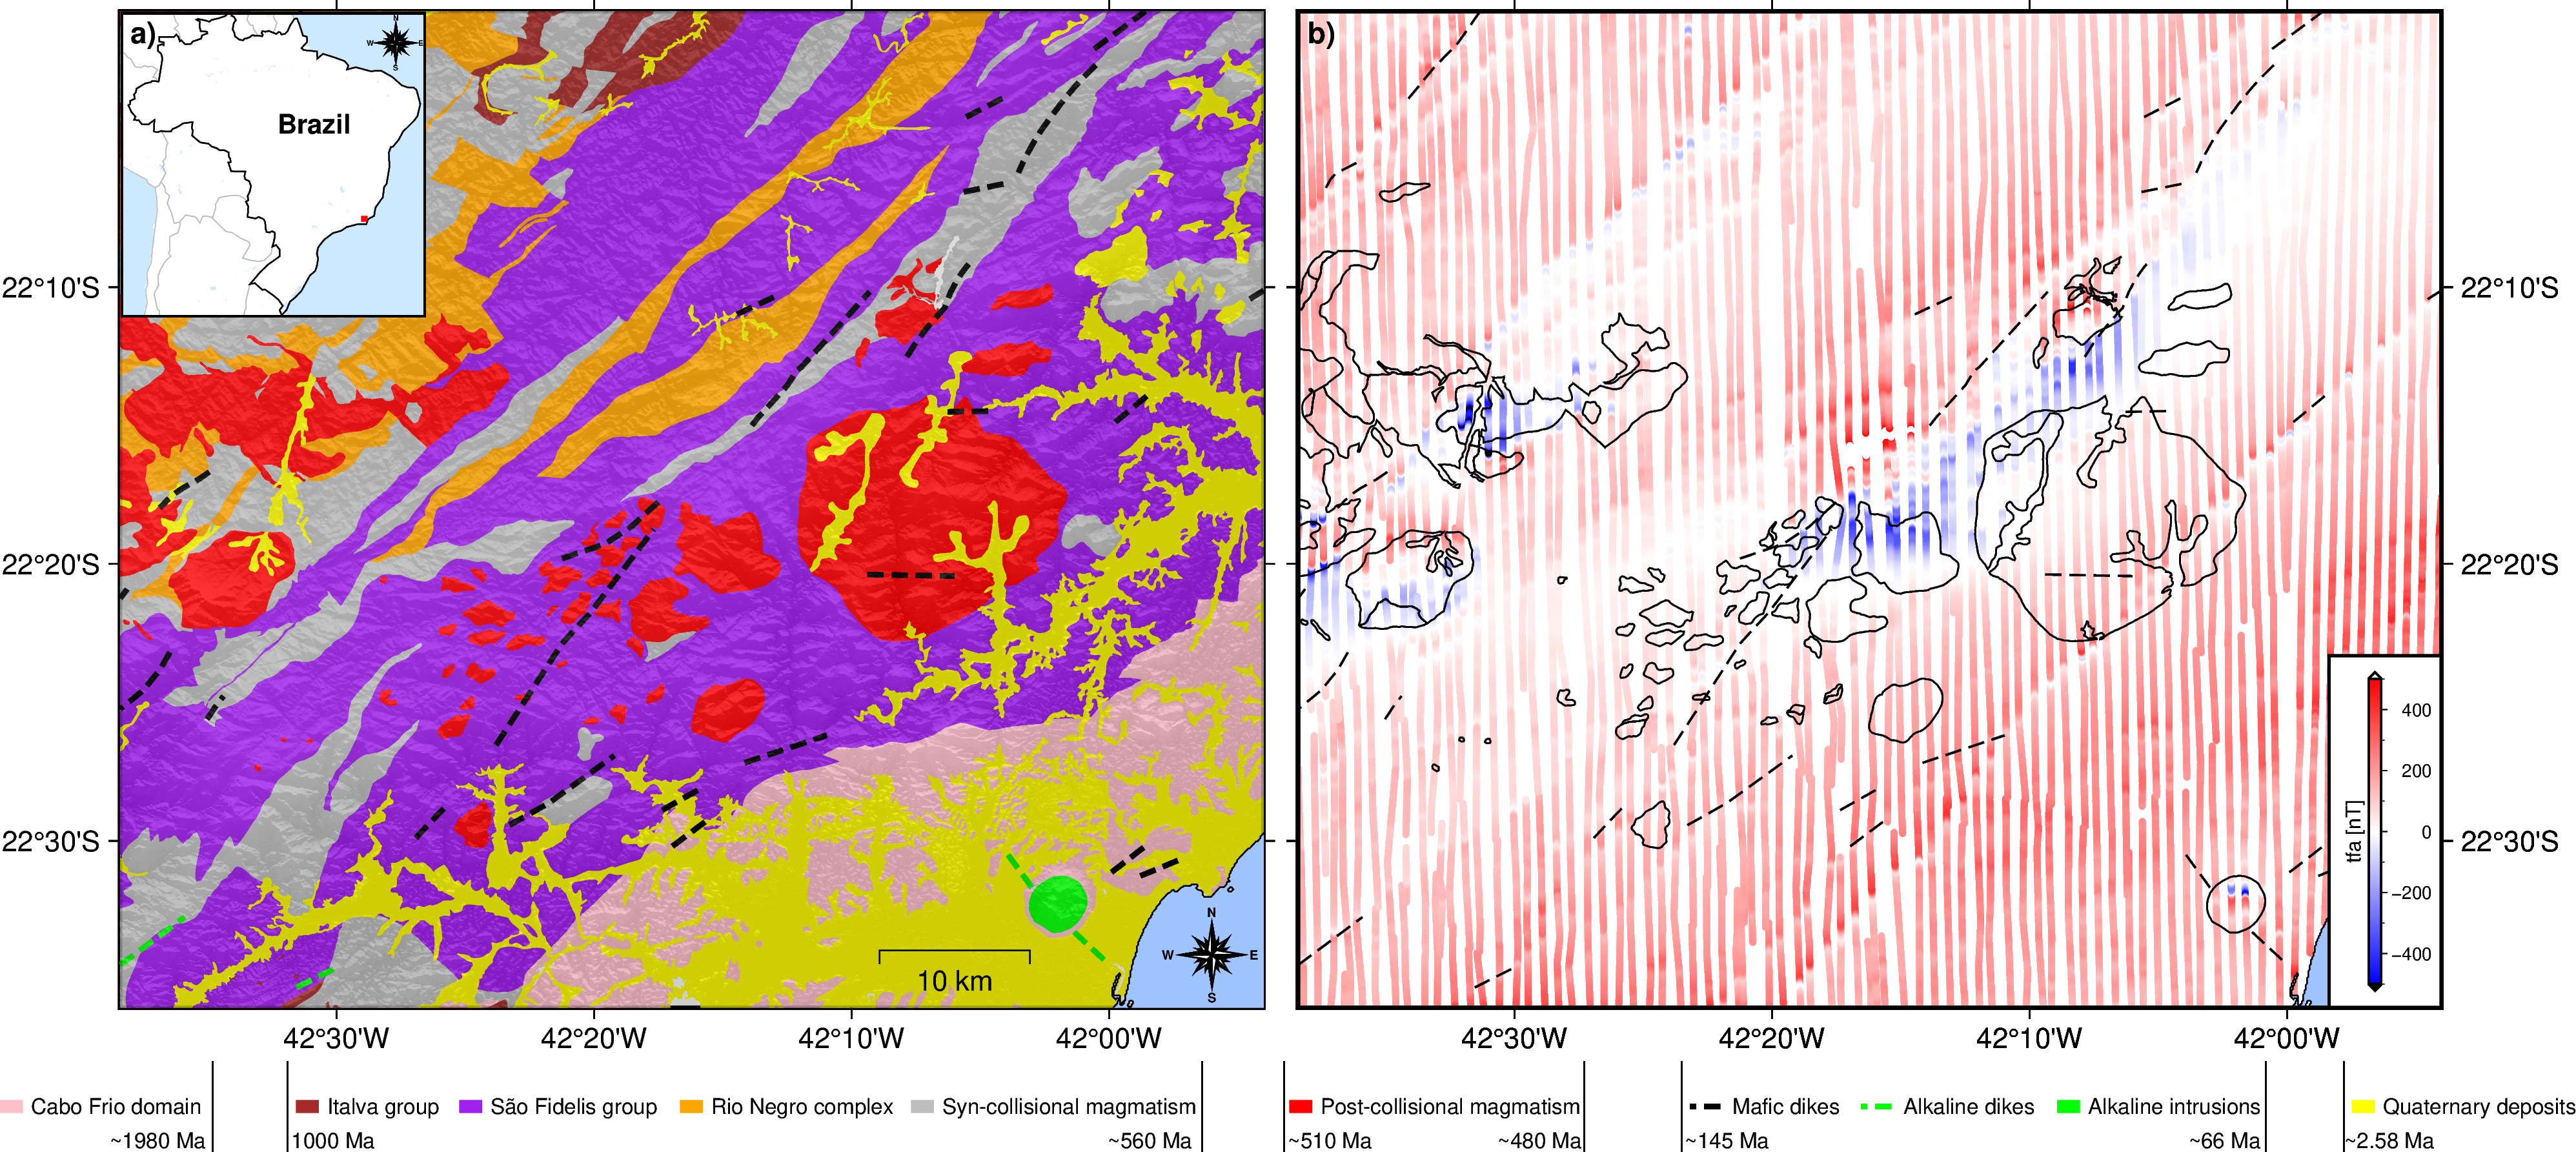
\includegraphics[width=1\linewidth]{euler-inversion/figures/real-data-geology.png}
\caption{
  Geologic map and observed total-field magnetic anomaly data from the west of
  the state of Rio de Janeiro, Brazil.
  a) Simplified geologic map showing the main groups and dykes that outcrop in
  the region.
  In pink is the Cabo Frio domain, dark red is the Italva group, purple is the
  São Fidelis group, orange is the Rio Negro complex, gray is the
  syn-collisional magmatism, red is the post-collisional magmatism, green are
  alkaline intrusions, yellow are the Quaternary deposits, and the dashed lines
  are mafic and alkaline dykes.
  b) The aeromagnetic flight-line data, overlaid by the outlines of the
  post-collisional magmatism and alkaline intrusions (solid black lines) and
  dykes (dashed lines).
  The geologic map was modified from \citet{Heilbron2016} and
  \citet{Dantas2017}.
}
\label{fig:rio_context}
\end{figure}

\begin{figure}[tb!]
\centering
\includegraphics[width=1\linewidth]{euler-inversion/figures/real-data-application.png}
\caption{
    Results of applying Euler inversion with a window size of \RioWindowSize{}
    and a window step of \RioWindowStep{} to the aeromagnetic data from Rio de
    Janeiro, Brazil.
    Estimated source locations and structural indices obtained from Euler
    inversion are shown as triangles ($\eta=1$), squares ($\eta=2$), and
    circles ($\eta=3$).
    The colour of each symbol represents the estimated depth below the surface
    of the Earth (topography).
    Also shown are the total-field anomaly flight-line data, the contours of
    the post-collisional magmatism and alkaline intrusions (solid black lines)
    and dykes (dashed lines).
    The purple squares highlight the A, B, C, and D anomalies that are
    discussed in the text.
}
\label{fig:rio_results}
\end{figure}

\begin{figure}[tb!]
\centering
\includegraphics[width=1\linewidth]{euler-inversion/figures/real-data-application-comparison.png}
\caption{
    Results of applying Euler deconvolution and finite-difference Euler
    deconvolution with a window size of \RioWindowSize{} and a window step of
    \RioWindowStep{} to the aeromagnetic data from Rio de Janeiro, Brazil.
    a-c) Euler deconvolution results with structural index $\eta=1$, $\eta=2$,
    and $\eta=3$, respectively.
    d) Finite-difference Euler deconvolution results.
    The structural index of the solutions are represented by pentagons
    ($\eta=-1$),  diamonds ($\eta=0$),  triangles ($\eta=1$),  squares
    ($\eta=2$), and circles ($\eta=3$).
    For finite-difference Euler deconvolution, the structural index symbol is
    that of the closest integer to the estimated value.
    The colour of each symbol represents the estimated depth below the surface
    of the Earth (topography).
    Also shown are the total-field anomaly flight-line data, the contours of
    the post-collisional magmatism and alkaline intrusions (solid black lines)
    and dykes (dashed lines).
}
\label{fig:rio_comp}
\end{figure}

The geology of Rio de Janeiro state (Southeastern Brazil) consists primarily of
high-grade metamorphic rocks and granitoid magmatism related to the Ribeira
Belt (RB) \citep{Heilbron2020}.
Figure~\ref{fig:rio_context}a shows a simplified geologic map of the area,
which was modified from \citet{Heilbron2016} and \citet{Dantas2017}.
The Ribeira Belt is traditionally interpreted as a thrust
belt formed by diachronous collisions mainly between the São Francisco and
Congo paleocontinents \citep{Heilbron2008, Trouw2000} or by an intracontinental
orogeny \citep[\textit{e.g.}][]{Meira2015, Meira2019}, during the Brasiliano
orogeny. This process culminated in an orogen-parallel, steep strike-slip shear
system \citep{EgydioSilva2005}, which deformed the Paleoproterozoic basement
rocks and reworked the Meso- to Neoproterozoic metasedimentary units (for
example, the Italva and São Fidelis groups) and syn-orogenic granitoid plutons
(for example, the Rio Negro complex) which formed during the orogeny
\citep{Heilbron2003, Heilbron2020}.
These tectonic events imprinted a distinct NE-ENE-trending structural pattern
onto these rocks.

The late Neoproterozoic to Cambrian period witnessed post-orogenic magmatism
\citep[\textit{e.g.,}][]{Valeriano2011}, marking the final stages of the West
Gondwana amalgamation. After this, the region remained tectonically quiescent
until the Lower Cretaceous, when reactivation occurred with the emplacement of
the NE-trending Serra do Mar mafic dyke swarm, preceding the break-up of West
Gondwana and the opening of the South Atlantic Ocean \citep{Almeida2013}.
Lastly, thermal anomalies in the region during the Upper Cretaceous to
Paleocene period led to the emplacement of alkaline complexes and dykes
\citep{Thompson1998}.
The geological complexity of the Ribeira Belt, marked by the interplay of
diverse tectonic regimes and magmatic events (Figure~\ref{fig:rio_context}a),
makes the Rio de Janeiro region an ideal test case for Euler inversion.

We used aeromagnetic data from the state of Rio de Janeiro which are
distributed by the Serviço Geológico do Brasil
(\url{https://geosgb.sgb.gov.br}). The data were collected in two phases:
Subarea 1 was surveyed between March 25 and May 27, 1978, using an Islander
aircraft (PT-KRP), while Subarea 2 was surveyed between April 6 and
July 19, 1978, using a Bandeirante aircraft (PT-GKJ), both funded by the
Brazilian government. As shown in Figure~\ref{fig:rio_context}b, the survey
followed a pattern of north-south flight lines spaced approximately
\qty{1}{\km} apart, with east-west tie lines.
Data were recorded at 100-meter intervals using a Geometrics G-803
magnetometer. Some of the notable features of the data are the NE-SW linear
features (interpreted here as dykes), which coincide with known dyke outcrops,
and complex dipolar anomalies which coincide with some of the post-collisional
magmatism and alkaline intrusions. A subset of \RioNData{} data points were
used in our analysis.

The data were not interpolated on a regular grid to avoid any smoothing effects
that the interpolation might have on the linear features. This could result in
an over-estimation of their depth, as discussed in Section~\ref{sec:windows}.
Instead, we used the gradient-boosted equivalent sources method of
\citet{Soler2021} to fit a model to the observed line data.
We then used the model to make predictions of the three spatial derivatives at
the original measurement locations by a central-difference method with
a coordinate shift of \RioDerivSpacing{}. Further details about the data
processing can be found in the source code archive that accompanies this
article \url{https://doi.org/\ArchiveDOI} \citep{figshare}.

We performed the moving-window Euler inversion (Algorithm~\ref{alg:window} and
Algorithm~\ref{alg:si} with $\eta_{min}=\RioSIMin$ and
$\eta_{max}=\RioSIMax$) on the observed total-field anomaly line data using
windows of size of \RioWindowSize{} which were moved \RioWindowStep{} at
a time.
The proportion of solutions kept was $\gamma=0.15$.
The inversion was performed with data weights of \RioWeightsF{} for the
total-field anomaly, \RioWeightsE{} for the eastward derivative, \RioWeightsN{}
for the northward derivative, and \RioWeightsU{} for the upward derivative.
To aid in the geological interpretation of the results, we converted the
estimated upward source coordinates $z_o$ to depths below the surface of the
Earth. We did so by subtracting the estimated $z_o$ from the interpolated
topographic height of the Shuttle Radar Topography Mission
\citep[SRTM;][]{SRTM}. The estimated positions and structural indices are shown
in Figure~\ref{fig:rio_results}.
We also performed Euler deconvolution with structural indices one, two, and
three, as well as finite-difference Euler deconvolution on the same dataset
using the same window size and window step for the sake of consistency.
These results are shown in Figure~\ref{fig:rio_comp}.

The Euler inversion estimated source positions shown in
Figure~\ref{fig:rio_results} highlight the NE-SW lineaments as well as some of
the more dipolar anomalies.
The lineaments are estimated with a mix of $\eta=1$, $\eta=2$, and $\eta=3$.
The southernmost lineament is mostly estimated with $\eta=1$ and depths
suggesting that it does not outcrop in its southernmost parts (depths of
\qtyrange{400}{600}{\m}), which is consistent with the geologic information in
Figure~\ref{fig:rio_context}a. The southernmost part of this lineament, in
particular, has an estimated $\eta=3$, which is known to happen for deeper
dykes in our synthetic data tests (Section~\ref{sec:windows}). Conversely, the
northernmost part of the lineament has a larger prevalence of $\eta=1$ with
shallower depths which coincide with a known dyke outcrop.
Other known dyke outcrops coincide with estimated sources with $\eta=1$,
however their depths range from \qtyrange{100}{300}{\m}. This may be caused by
an excess of smoothing in the vertical derivative or effects of noise in the
estimated coordinates. The lineaments in the northwestern part of the region
are also highlighted by estimated sources.
However, their structural indices are a mix of $\eta=2$ and $\eta=3$,
suggesting deeper sources. This is inline with the geologic information, which
includes no outcrops of linear structures in the area.

The dipolar anomalies are associated with post-collisional and alkaline
intrusions, many of which are also cut by known outcropping dykes or have known
dykes with magnetic signals that significantly overlap with the dipolar
anomalies. The Euler inversion estimated structural indices for them range from
$\eta=2$ to $\eta=3$. We have highlighted four dipolar anomalies, marked as A,
B, C, and D in Figure~\ref{fig:rio_results}, to aid in our discussion.

\begin{itemize}
\item \textbf{Anomaly A:} Has a reversed polarity and linear feature to its
    north that is not associated with any known dyke outcrop. The linear
    feature is highlighted by Euler inversion estimates with $\eta=1$ and depth
    of \qtyrange{300}{400}{\m}, which can be interpreted as a non-outcropping
    dyke. The dipolar anomaly itself has Euler inversion solutions with
    $\eta=3$ and depth of \qtyrange{1000}{2000}{\m}.
    The solutions in the centre of the anomaly present a shallower depth than
    the solutions to the north and south of the anomaly centre. From the
    results on synthetic data in Section~\ref{sec:windows}, we can interpret
    the depth range to be caused by the moving window procedure and the effect
    of interfering sources. The depth to the centre of the anomaly source is
    likely close to \qty{1000}{\m}.

\item \textbf{Anomaly B:} The dipolar anomaly is likely associated with
    a non-outcropping portion of the post-collisional magmatism. The anomaly is
    cut by several NE-SW linear features, some of which overlap with known dyke
    outcrops. The linear feature to the north is associated with Euler
    inversion results with $\eta=1$ and depths ranging from
    \qtyrange{300}{600}{\m}, suggesting a non-outcropping dyke. At the centre
    of the anomaly are Euler inversion estimates with $\eta=3$ and depth
    estimate of approximately \qty{1400}{\m}. The Euler inversion solutions
    surrounding these central solutions are likely caused by interference from
    other sources.

\item \textbf{Anomaly C:} A dipolar anomaly associated with an outcropping
    portion of the post-collisional magmatism. There is a known outcropping
    dyke to the south of the anomaly, which is associated with Euler inversion
    estimates with $\eta=1$ and depths ranging from \qtyrange{500}{1000}{\m}.
    These depth estimates are likely overestimated because of the interference
    of the dipolar anomaly. The main anomaly has Euler inversion solutions with
    $\eta=2$ and $\eta=3$ and depths varying from \qtyrange{1400}{1800}{\m}.
    There is no clear indication of which of these estimates is more reliable.

\item \textbf{Anomaly D:} A small dipolar anomaly associated with an
    outcropping alkaline intrusion. The Euler inversion estimates have $\eta=3$
    and depths \qtyrange{1700}{2000}{\m}. There are known outcropping dykes
    around the main intrusion but they have no discernible magnetic anomalies
    and no Euler inversion solutions associated with them.
\end{itemize}

Overall, the Euler inversion solutions in Figure~\ref{fig:rio_results} are
consistent with the known geology in Figure~\ref{fig:rio_context}a.
The main linear features are mostly associated with Euler inversion estimates
with $\eta=1$ and shallow depths, particularly where known dyke outcrops are
located.
Deeper linear features are estimated with $\eta=2$ and $\eta=3$, which is
consistent with the synthetic data results (Section~\ref{sec:windows}).
The dipolar anomalies have consistent Euler inversion estimates with $\eta=3$
when they are well isolated from interfering sources.
Otherwise, they are estimated with a mix of structural indices and depths, as
was demonstrated in Section~\ref{sec:windows}.

When compared to the Euler deconvolution and finite-difference Euler
deconvolution results (Figure~\ref{fig:rio_comp}), the Euler inversion results
are less dispersed and better delinear the linear features present in the data.
The structural index results from finite-difference Euler deconvolution
(Figure~\ref{fig:rio_comp}d) are underestimated, with most values of $\eta$
being less than one, which is not in accordance with the geology of the area.

%%%%%%%%%%%%%%%%%%%%%%%%%%%%%%%%%%%%%%%%%%%%%%%%%%%%%%%%%%%%%%%%%%%%%%%%%%%%%%%
\section{Conclusion}

Euler deconvolution is a widely used method for locating the sources of
potential-field data.
It has its limitations in real-world scenarios due to its dependence on the
chosen value of the structural index $\eta$ and its sensitivity to
high-frequency noise and signal overlap from interfering sources.
We have developed a new method to solve Euler's homogeneity equation for the
source position, base level, and integer structural index, which we call
\textit{Euler inversion}.
Unlike Euler deconvolution, Euler inversion is also able to estimate the
predicted field and its spatial derivatives, as well as assign different
weights to each type of data.
Our method can be applied to gridded and non-gridded data, which can
be useful to limit the effects of smoothing from interpolation in the final
results when the original data have large spacing between flight lines.
The Euler inversion algorithm is computationally efficient because most of the
large matrices involved in the computations are diagonal or block-diagonal.
We found that, in practice, the computation time of Euler inversion and Euler
deconvolution are on the same order of magnitude.

Tests on synthetic data show that Euler inversion outperforms Euler
deconvolution and finite-dif\-fer\-ence Euler deconvolution (a variant that
estimates $\eta$ but does not rely on second-order derivatives) in terms of
robustness to random noise and interfering sources inside the data window.
Our tests also show that the estimated $z_o$ coordinate is correlated with the
structural index, as is the case for Euler deconvolution.
We have also found that the data misfit from Euler inversion is minimal when
the integer structural index used is equal or close to the true one for
idealized sources.
This led us to develop an algorithm for estimating the best integer structural
index based on the data misfit.
A test on complex synthetic data from a model of dykes and dipoles with
overlapping signals shows that Euler inversion is able to estimate the
structural index and position of the sources within expected error bounds when
the signal overlap is not larger than the data window.
For deeper dykes in particular, Euler inversion was not able to estimate the
correct $\eta=1$, leading to an overestimation of the depths.

We applied Euler inversion to an aeromagnetic dataset from Rio de Janeiro,
Brazil, to analyse its performance under real-world scenarios.
Euler inversion was able to locate the NE-SW linear features in the data with
an $\eta=1$ which are associated with known dyke outcrops.
For the deeper linear features, Euler inversion was not able to estimate the
correct $\eta=1$.
Some of the dipolar anomalies present in the data were picked out with
$\eta=3$, while the sources with a large signal overlap with other features
provided a mix of $\eta=2$ and $\eta=3$.
These results are consistent with the synthetic data tests and show the
benefits and limitations of the proposed method.

Euler inversion outperforms Euler deconvolution and finite-difference Euler
deconvolution in most cases.
Its reduced sensitivity to noise and interfering sources, in particular,
may prove beneficial for magnetic microscopy studies, in which high-frequency
noise and interference from multiple dipolar sources are a significant hurdle
\citep{Souza-Junior2024}.
However, it still suffers from some of the same limitations.
While Euler inversion is less sensitive to signal overlap, it still fails to
correctly estimate the position and structural index when the overlap is large.
The windowing procedure still generates a large amount of spurious solutions
which need to be filtered out.
This could be improved with techniques like the source detection method
proposed by \citet{Castro2020}, for example.
Euler inversion can also be coupled with other inverse problems by following
our methodology to add Euler's equation as a non-linear constraint.
This could help with issues of non-uniqueness and stability in traditional 3D
inverse problems in potential-field methods.

As is the case with other Euler deconvolution-based methods, Euler inversion
also suffers from instability when sources are 2D \citep{Mushayandebvu2004}
and a lack of support for sources that are defined by multiple points, for
example steps which have a top and bottom \citep{Gerovska2010}.
The issue of instability was evident in our synthetic data tests which
simulated dykes and did not contaminate the data with random noise.
However, both in the synthetic data tests with noise and the real data
application, this did not appear to be a significant issue.
In both cases, Euler inversion was better at outlining the 2D sources than
Euler deconvolution.
Nonetheless, it would be worthwhile to investigate this issue further and
explore the use of regularization and an adaptation of the method of
\citet{Mushayandebvu2004} to the Euler inversion mathematical formulation.
A thorough comparison of Euler inversion with the Similarity Transform-based
methods, like \citet{Gerovska2010}, would also be worth pursuing.
Euler inversion could complement such methods, which often require gridded
data, in cases where data are of poor quality or flight-line spacing is large.


%%%%%%%%%%%%%%%%%%%%%%%%%%%%%%%%%%%%%%%%%%%%%%%%%%%%%%%%%%%%%%%%%%%%%%%%%%%%%%%
\section*{Data availability statement}

The Python source code and data that were used to produce all results and
figures presented here are available at
\url{https://github.com/\GitHubRepository}
and \url{https://doi.org/\ArchiveDOI} \citep{figshare}
under the CC-BY license and the MIT license.
This study made use of the following open-source scientific software:
matplotlib \citep{Hunter2007} and PyGMT \citep{pygmt} for generating figures
and maps,
Numpy \citep{numpy} and Scipy \citep{scipy} for linear algebra,
Pandas for manipulating tabular data \citep{McKinney2010,pandas},
GeoPandas for reading and plotting shapefiles \citep{geopandas},
pyproj for data projection \citep{pyproj},
xarray \citep{xarray} for working with gridded data,
Verde \citep{verde2018} for moving windows and interpolation,
and Harmonica \citep{harmonica} for potential-field data processing and
modeling.
The aeromagnetic and geologic data are available from Serviço Geológico do
Brasil (\url{https://geosgb.sgb.gov.br}) under a CC-BY-NC license.
The magnetic data are part of survey 1038 ``Projeto Aerogeofísico São Paulo --
Rio de Janeiro''.
Both are also available in our source code and data archive \citep{figshare}.


%%%%%%%%%%%%%%%%%%%%%%%%%%%%%%%%%%%%%%%%%%%%%%%%%%%%%%%%%%%%%%%%%%%%%%%%%%%%%%%
\section*{Acknowledgements}

We are indebted to the developers and maintainers of the open-source software
without which this work would not have been possible.
We thank Dr. Valéria C. F. Barbosa for many insightful discussions over the
years which helped shape our research.
We are grateful to editor Dr. Kosuke Heki and reviewers Dr. Alan B. Reid and
Dr. Saulo Oliveira for their constructive comments.
LU would like to thank Prof. Spiros Pagiatakis for being an incredible
instructor and teaching him the mathematics which formed the foundations of
this work during his undergraduate exchange at York University.
LU was supported in part by start-up grant PRPI 22.1.09345.01.2 from
Universidade de São Paulo.
GFSJ was supported by scholarship 2021/08379-5 from the Fundação de Amparo
à Pesquisa do Estado de São Paulo (FAPESP).
The opinions, hypotheses, and conclusions or recommendations expressed in this
material are the responsibility of the authors and do not necessarily reflect
the views of FAPESP.

\section*{CRediT author contributions}

\textbf{Leonardo Uieda:} Conceptualisation, Data curation, Formal analysis,
Investigation, Methodology, Pro\-ject administration, Resources, Software,
Supervision, Visualisation, Writing – original draft.

\noindent
\textbf{Gelson Ferreira Souza-Junior:} Data curation, Formal analysis,
Resources, Software, Visualisation, Writing - original draft, Writing - review
\& editing.

\noindent
\textbf{India Uppal:} Data curation, Formal analysis, Investigation, Software,
Writing - review \& editing.

\noindent
\textbf{Vanderlei Coelho Oliveira Jr.:} Conceptualisation, Methodology, Writing
- review \& editing.

\endgroup

%==============================================================================
\chapter{Conclusion}

Bla.


%%%%%%%%%%%%%%%%%%%%%%%%%%%%%%%%%%%%%%%%%%%%%%%%%%%%%%%%%%%%%%%%%%%%%%%%%%%%%%%
\bibliographystyle{apalike-doi}
\bibliography{references}

\end{document}
